% указываем класс документа
%\documentclass[twoside,8pt,a5paper,openany]{report}
\documentclass[twoside,10pt,a5paper,openany]{report}

% подключаем собственный стилевой файл
\usepackage{labstyle}
\usepackage{labstyle2}







\makeindex





\begin{document}

% указываем язык (для автоматической вставки слов, типа "Глава", "Содержание", "Литература", "рис." и пр.
\selectlanguage{ukrainian}
\def\chaptername{Лабораторна робота №}


% подключаем файлы содержимого
\begin{titlepage}
\newpage

\begin{center}
МІНІСТЕРСТВО ОСВІТИ І НАУКИ, МОЛОДІ ТА СПОРТУ УКРАЇНИ \\

ХЕРСОНСЬКИЙ НАЦІОНАЛЬНИЙ ТЕХНІЧНИЙ УНІВЕРСИТЕТ \\*

КАФЕДРА ІНФОРМАЦІЙНИХ ТЕХНОЛОГІЙ

\end{center}


\vspace{8em}

\begin{center}
\Large Методичні вказівки до лабораторних робіт \\ з курсу дисципліни
\end{center}

\vspace{2.5em}

\begin{center}
\huge{\textbf{<<Web-програмування>>}}
\end{center}

\vspace{1em}

\textbf{
\begin{center}
Увага! Роботу над методичними вказівками не завершено, вже існуючі завдання змінюватись не будуть, але у теоретичному матеріалі та додатках зміни можливі.
\end{center}
}
\vspace{\fill}

\begin{center}
Херсон 2012
\end{center}

\end{titlepage}



% ненужное можно просто закомментировать знаком процента "%" 

% первую страницу не нумеруем
%\thispagestyle{empty}			

% название
%\title{Методичні вказівки до лабораторних робіт з дисципліни <<web-програмування>>}
%\author{Жарікова М.В., Левицький В.М.}
%\maketitle

% печатаем содержание
%\chapter*[Зміст]{Зміст}
\tableofcontents

% ничанаем с новой страницы
%\newpage

% печатаем перечень рисунков
%\chapter*{Перелік ілюстрацій}
\listoffigures

% печатаем перечень таблиц
%\chapter*{Перелік таблиць}
\listoftables

\lstlistoflistings

%\lstlistoflistings


%\chapter{Основи мережі Internet}
\nopagebreak[4]
\section*{Мета роботи}
Вивчити основи роботи мережі Інтернет. Ознайомитись з роботою протоколу НТТР. Навчитися встановлювати необхідне програмне забезпечення для розробки сценаріїв на РНР.
\nopagebreak[4]
\section{Структура мережі Internet}
\nopagebreak[4]

\textbf{Інтернет}\index{Мережі!Internet}~--- всесвітня інформаційна комп'ютерна мережа, що являє собою об'єднання безлічі регіональних комп'ютерних мереж і комп'ютерів, що обмінюються один з одним інформацією по каналах громадських телекомунікацій (виділених телефонних аналогових і цифрових лініях, оптичним каналам зв'язку і радіоканалах, в тому числі супутникових лініях зв'язку). Комп'ютери, підключені до мережі Інтернет, можуть мати будь-які апаратні і програмні платформи, але при цьому вони повинні підтримувати стек протоколів (сімейство протоколів) зв'язку TCP/IP.

Інформація в Інтернет зберігається на серверах. Сервери мають свої адреси і управляються спеціалізованим серверним програмним забезпеченням, яке дозволяє пересилати пошту, файли, проводити конференції, тощо. 

Доступ окремих користувачів до інформаційних ресурсів Інтернету зазвичай здійснюється через провайдера або корпоративну мережу.

\textbf{Провайдер (ISP, Internet Service Provider)}\index{Мережі!Internet!провайдер}~--- постачальник мережевих послуг~--- особа або організація надають послуги з підключення до комп'ютерних мереж. В якості провайдера виступає деяка організація, що має модемний пул для з'єднання з клієнтами та виходу у всесвітню мережу. Користувачі підключаються до мережі через маршрутизатори місцевих постачальників послуг Інтернету, які мають постійне підключення до Інтернет через регіональних провайдерів. Регіональний провайдер, підключається до більшого провайдеру національного масштабу, що має вузли в різних містах країни.

Кожен комп'ютер, підключений до мережі Інтернет, має унікальну адресу. Адреси комп'ютерів бувають двох видів:
\begin{enumerate}
\item IP-адреса (обов'язкова)
\item DNS-имя (Domain Name System, доменне ім'я) 
\end{enumerate}
MAC-адреса не розглядається, оскільки у глобальній мережі вона не використовується для ідентифікації комп'ютерів.

\textbf{IP-адрес (Internet Protocol Address)}\index{Мережі!IP}~--— унікальна мережева адреса вузла в комп'ютерній мережі, побудованій на основі IP-протоколу. 
\textbf{IPv4-адреси} складаються з чотирьох байтів, тобто з 32-розрядного двійкового числа, яке для зручності поділяється на чотири блоки по 8 бітів.
\textbf{IPv6-адреси} відображаються як вісім груп по чотири шістнадцяткові цифри, розділені двокрапкою. Приклади IPv4 та IPv6 адрес:

\begin{verbatim}
IPv4: 192.0.2.235
IPv6: 2001:0db8:11a3:09d7:1f34:8a2e:07a0:765d
\end{verbatim}

IP-адреса складається з двох частин: номера мережі й номера вузла (комп'ютера) в мережі. Якщо окремий комп'ютер (хост-комп'ютер) або мережа є складовою частиною мережі Інтернет, то IP-адреса присвоюється організація ICANN (Інтернет корпорація з присвоєння імен і номерів)


\textbf{Доменне (DNS) ім'я}\index{Мережі!DNS}~--- символьне ім'я, що служить для ідентифікації областей~--- одиниць адміністративної автономії в мережі Інтернет~--- у складі вищестоящої по ієрархії такої області. Доменну адресу побудований на основі ієрархічної класифікації, тобто доменну адресу включає в себе кілька рівнів доменів, наприклад: \verb'google.com.ua'.
Домен верхнього рівня розташовується в імені правіше, а домен нижнього рівня~--- лівіше. Користувач мережі Інтернет працює не з IP-адресами, а тільки з доменними адресами. Перетворення доменного імені в IP-адресу здійснюють \textbf{DNS-сервера}.


Для повноцінної роботи в мережі передбачений ряд протоколів прикладного рівня. Протокол прикладного рівня~--- протокол верхнього (7-ого) рівня мережевої моделі OSI, забезпечує взаємодію мережі і користувача. Рівень дозволяє додаткам користувача мати доступ до мережевих служб, таким як обробник запитів до баз даних, доступ до файлів, пересилання електронної пошти. Також відповідає за передачу службової інформації, надає додаткам інформацію про помилки й формує запити до рівня подання. Приклад: HTTP, POP3, SMTP

\pagebreak[3]

\section{Передача даних через протокол HTTP}
\nopagebreak[4]

\textbf{Протокол передачі гіпертексту (Hypertext Transfer Protocol, HTTP)}\index{Мережі!HTTP}~--- протокол прикладного рівня для розподілених мультимедійних інформаційних систем.

Перші версії, такі, як HTTP/0.9, являли собою прості протоколи для передачі даних через Інтернет. Версія HTTP/1.0, поліпшила протокол, дозволивши використання повідомлень в форматі MIME, що містять метаінформацію про переданих даних, і модифікатори для запитів / відгуків.

Для опису характеру, найменування та місця розташування інформаційних ресурсів введені:
\index{Мережі!HTTP!URL/URI/URN} \textbf{URI~--- Uniform Resource Indicator} (уніфікований ідентифікатор ресурсу),
\textbf{URL~--- Uniform Resource Locator} (уніфікований визначник місцезнаходження ресурсу)
\textbf{URN~--- Unifrorm Resource Name} (уніфіковане ім'я ресурсу).
URI: Позначає ім'я та адресу ресурсу в мережі. Як правило ділиться на URL і URN, тому URL і URN це складові URI.

URL: Адреса деякого ресурсу в web. URL визначає місцезнаходження ресурсу і спосіб звертання до нього.

URN: Ім'я деякого ресурсу в web. Сенс URN в тому, що він визначає тільки назва конкретного предмета, який може знаходиться в безлічі конкретних місць.

Як приклад можна представити наступні посилання:
\begin{verbatim}
URI = http://handynotes.ru/2009/09/uri-url-urn.html
URL = http://handynotes.ru
URN = / 2009/09/uri-url-urn.html
\end{verbatim}
HTTP використовується також в якості базового протоколу для комунікації користувацьких агентів з проксі-серверами і іншими системами Інтернет, у тому числі й використовуючих протоколи SMTP, NNTP і FTP.

Всі HTTP-транзакції мають один загальний формат. Кожен запит клієнта і відповідь сервера складається з трьох частин: рядки запиту (відповіді), розділу заголовка і тіла. Клієнт ініціює транзакцію наступним чином:

\begin{enumerate}

\item Клієнт встановлює зв'язок з сервером на номер телефону порту (за замовчуванням~--- 80). Потім клієнт посилає запит документа, вказавши HTTP-команду, яка називається методом, адреса документа і номер версії HTTP. Наприклад, в запиті
\begin{verbatim}
GET / index.html HTTP/1.0
\end{verbatim}

\item Клієнт посилає інформацію заголовка (необов'язкову), щоб повідомити серверу інформацію про свою конфігурації і дані про формати документів, які він може приймати.
\begin{verbatim}
User-Agent: Mozilla/4.05 (WinNT; 1)
Accept: image/gif, image/x-xbitmap, image/jpeg, image/pjpeg, */*
\end{verbatim}

\item Надіславши запит і заголовки, клієнт може відправити і додаткові дані. Клієнти також можуть використовувати їх для приміщення відредагованій сторінки назад на Web-сервер.

\end{enumerate}

Сервер відповідає на запит клієнта наступним чином:

\begin{enumerate}

\item Перша частина відповіді сервера~--- рядок стану, що містить три поля: версію HTTP, код стану й опис. Поле версії містить номер версії HTTP, яку даний сервер користується для передачі відповіді.

Код стану~--- це триразрядне число, що позначає результат обробки сервером запиту клієнта. Опис, наступне за кодом стану, є просто зрозумілий для людини текст, що пояснює код стану. Наприклад, рядок стану \verb'НТТР/1.0 200 OK' говорить про те, що сервер для відповіді використовує версію HTTP 1.0. Код стану 200 означає, що запит клієнта був успішним і витребувані дані будуть передані після заголовків.
\item Після рядка стану сервер передає клієнтові інформацію заголовка, що містить дані про самого сервері і викликаній документі. Нижче наведено приклад заголовка:

\begin{verbatim}
Date: Fri, 10 Jan 1998 08:17:58 GMT
Server: Apache/1.2.6
Last-modified: Mon, 12 Jun 1997 21:53:08 GMT
Content-type: text/html
Content-length: 2482

\end{verbatim}

\item Якщо запит клієнта успішний, то надсилаються витребувані дані. Це може бути копія файлу або результат виконання CGI-програми. Якщо запит клієнта задовольнити не можна, передаються додаткові дані у вигляді зрозумілого для користувача роз'яснення причин, за якими сервер не зміг виконати даний запит.
\end{enumerate}

\pagebreak[3]

\section{Мови програмування для web, web-сервери, мережеві СКБД}
\nopagebreak[4]

\subsection*{Мови програмування}

Серверні мови web-програмування можуть бути умовно розділені по операційним системам, на яких вони працюють: Windows і *nix. Це розділення в деякій мірі умовно, тому що практично всі популярні мови і фреймворки портовано на усі популярні сімейства ОС. Тим не менш, вони рідко використовуються на нерідних ОС.

Якщо говорити про ОС Windows, то тут панує технологія
\textbf{ASP.NET}, \index{Мови програмування!ASP.NET}розроблена компанією Microsoft. За допомогою ASP.NET можна створювати сайти будь-якого рівня складності~--- від найпростіших, що складаються їх декількох сторінок, до дуже складних, що обробляють мільйони запитів на день.

Самим популярним мовою web-програмування є, безумовно,
\textbf{PHP}. \index{Мови програмування!PHP}Його основними перевагами є: простий синтаксис, висока швидкодія, підтримка більшістю хостингів. Дуже вагомою перевагою є те, що на PHP написано багато популярних CMS.

\textbf{Perl}\index{Мови програмування!Perl}~--- це інтерпретована мова програмування. Завдяки цьому, грамотно написаний Perl-скрипт може працювати як в *nix, так і в Windows, як на процесорах x86, так і на Alpha-або Power PC.

\textbf{JSP (Java Server Pages)}\index{Мови програмування!Java Server Pages}~--- це частина технології J2EE, призначена для створення сайтів за допомогою мови Java. JSP має дуже багато спільного з ASP.NET і вибір між цими двома технологіями найчастіше ґрунтується на суб'єктивних перевагах та досвіду роботи з якоюсь іх технологій.

Останнім часом високу популярність придбав мову
\textbf{Ruby}\index{Мови програмування!Ruby} і, зокрема, фреймворк
\textbf{Ruby On Rails}. З його допомогою можна дуже швидко створити сайт з необхідною функціональністю. Одним з істотних недоліків Ruby, є низька швидкодія.

Мова програмування
\textbf{Python}\index{Мови програмування!Python} сьогодні є одною із самих популярних інтерпретованих мов. Python, що є об'єктно-орієнтованою мовою, відмінно справляється з найрізноманітнішими завданнями, а міжплатформенність для цієї мови реалізована в повному обсязі.


\subsection*{Web-сервери}


На даний момент найбільш поширеним web-сервером, що займає більше 65\% ринку, є
\textbf{Apache}\index{Web-сервери!Apache}~--- безкоштовний web-сервер, найбільш часто використовується в UNIX-подібних операційних системах.

У середовищі Windows, дуже поширений
\textbf{IIS (Internet Information Services)}\index{Web-сервери!IIS} від компанії Microsoft, розповсюджуваний з серверними версіями ОС.

\textbf{Nginx}\index{Web-сервери!Nginx}~--- перспективний web-сервер і поштовий проксі-сервер, розроблений для Unix-подібних операційних системах. Починаючи з версії 0.7.52 з'явилася бінарна збірка під Microsoft Windows.

\textbf{Lighttpd}\index{Web-сервери!Lighthttpd}~--- компактний web-сервер, розроблений для Unix-подібних операційних систем, портований надалі на платформу Windows.
\textbf{Google Web Server (GWS)}\index{Web-сервери!GWS}~--- web-сервер, який використовується Google для організації своєї web-інфраструктури.


\subsection*{Мережеві СКБД}


Реляційна модель баз даних являє собою централізоване сховище таблиць, що забезпечує безпечний одночасний доступ до інформації з боку багатьох користувачів. У рядках таблиць частина полів містить дані, що відносяться безпосередньо до запису, а частина~--- посилання на записи інших таблиць. Таким чином, зв'язки між записами є невід'ємною властивістю реляційної моделі.

Кожен запис таблиці має однакову структуру. Наприклад, у таблиці, яка містить описи автомобілів, у всіх записів буде один і той же набір полів: виробник, модель, рік випуску, пробіг і т.д. Такі таблиці легко зображувати в графічному вигляді.

В реляційній моделі СКБД досягається інформаційна та структурна незалежність. Записи не пов'язані між собою настільки, щоб зміна однієї з них торкнулося інші, а зміни структура СКБД, бази даних не обов'язково призводить до перекомпіляції працюючих з нею додатків.
Для побудови сайтів використовують багатокористувацькі реляційні СКБД з підтримкою SQL. Як правило це \index{СУБД}
\textbf{MS SQL Server}, 
\textbf{MySQL, Oracle}, 
\textbf{Interbase}, 
\textbf{DB2} або 
\textbf{PostgreSQL}. Вибір конкретної СКБД залежить від призначення сайту, планованих обсягів бази даних, навантаження на сервер, оптимальної для програміста ліцензії. Величезний відсоток web-хостингів базується на використанні MySQL і PostgreSQL. Цей вибір обумовлений широкими можливостями, наданими даними продуктами, а також їх вартістю.

\pagebreak[3]

\section{Налаштування web-сервера Apache}
\nopagebreak[4]
Завантажити Apache можна з дзеркал наведених на офіційному сайті \verb'http://www.apache.org/'. При пошуку слід пам'ятати, що Apache так само може називатися HTTPD, на ім'я його демона в UNIX. На дзеркалах зазвичай багато різних файлів, необхідно скачати бінарний файл для Windows *.exe або *.msi. У випадку якщо у вас система *nix-сімейства вам необхідно встановити пакет httpd потрібної версії з вашого репозиторію.
Інсталяція програмного пакету для Windows не змінюється вже багато років (Рис.~\ref{f1-1:image}). 
\begin{figure}
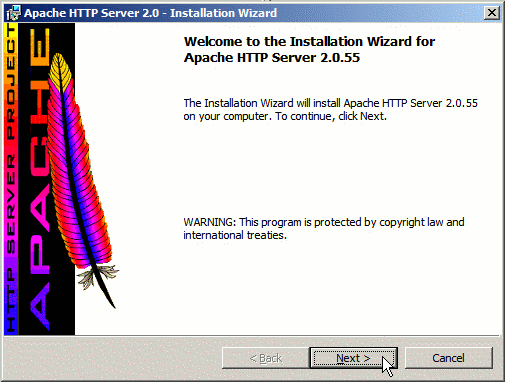
\includegraphics[scale=1,width=8cm]{ch01-01.png}
\caption{Інсталятор Apache}
\label{f1-1:image}
\end{figure}
Вам потрібно буде занести домен, в якому знаходиться сервер, ім'я сервера, e-mail адміністратора сервера. У даному випадку ці дані не важливі, їх можна залишити стандартними  (Рис.~\ref{f1-2:image}).
\begin{figure}
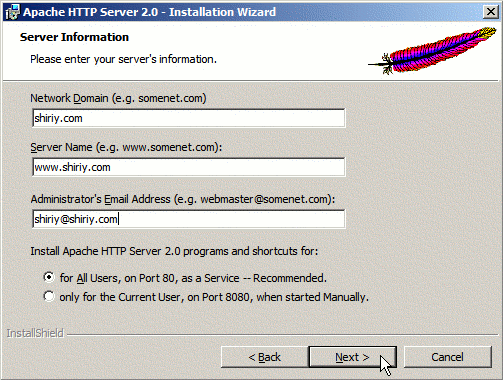
\includegraphics[scale=1,width=8cm]{ch01-02.png}
\caption{Налаштування доменних імен}
\label{f1-2:image}
\end{figure}
Також треба вибрати каталог, куди буде встановлюватися Apache, або залишити його стандартним  (Рис.~\ref{f1-3:image}). 
\begin{figure}
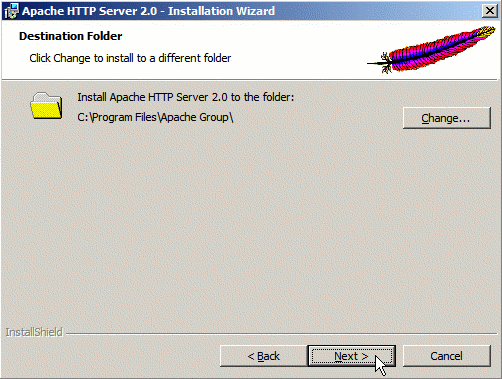
\includegraphics[scale=1,width=8cm]{ch01-03.png}
\caption{Каталог розміщення Apache}
\label{f1-3:image}
\end{figure}
Подальші зміни в конфігурації Apache можна вносити, використовуючи файл <<httpd.conf>>.

Щоб було зручно маніпулювати файлами ваших проектів створіть папку зі зрручним для вас коротким шляхом, наприклад \verb'D:\Site', в якій будуть зберігатися всі інші програми і дані сайту. Далі створіть папку \verb'D:\Site\localhost\', в якій створіть директорії WWW і CGI відповідно. WWW міститиме матеріали сайту, а CGI - скрипти CGI, якщо такі у вас будуть. В директорії \dots\verb'\Apache2\Conf\' знайдіть файл <<httpd.conf>>~--- це файл з налаштуваннями. У ньому знайдіть рядок

\begin{verbatim}
ServerRoot "C :/Program Files/Apache Group/Apache2"
\end{verbatim}

Він повинна містити шлях до самого Апач, тобто на ту папку, куди у вас Апач встановлений. Зверніть увагу, що в шляху слеш прямий і закінчується адреса без слеша.

Далі прив'язуємо Apache до конкретного порту:

\begin{verbatim}
Listen 80
\end{verbatim}

При деяких помилках сервера Apache відсилає електронні листи адміністратору, адреса поштової скриньки налаштовується у рядку

\begin{verbatim}
ServerAdmin your@email.name
\end{verbatim}

Тепер прописуємо шлях до даних сайту

\begin{verbatim}
DocumentRoot "D:/Site/localhost/WWW"
\end{verbatim}

Знайдіть блок 
\begin{verbatim}
<Directory "C:/Program Files/Apache Group/Apache2/htdocs">
\end{verbatim}

і замініть його на

\begin{verbatim}
<Directory "D:/Site">
    Options Indexes Includes
    AllowOverride All
    Order allow,deny
    Allow from all
</Directory>
\end{verbatim}

\pagebreak[3]

\section{Налаштування PHP}
\nopagebreak[4]
Встановлення PHP в середовищі Windows також не створює проблем. Завантажте встановлювач і запустіть його. 

Необхідно буде вибрати каталог для встановлення інтерпретатору, встановлену версію Apache (Рис.~\ref{f1-4:image}).
\begin{figure}
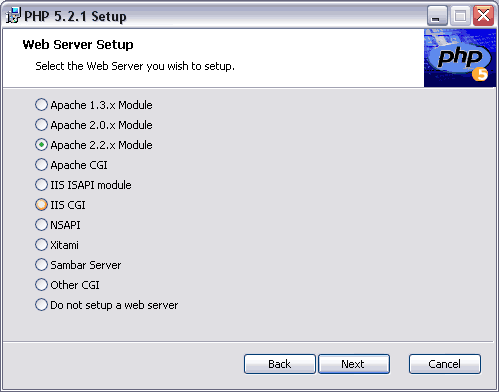
\includegraphics[scale=1,width=8cm]{ch01-04.png}
\caption{Каталог розміщення PHP}
\label{f1-4:image}
\end{figure}
Також необхідно задати місцезнаходження файлу  <<httpd.conf>> (Рис.~\ref{f1-5:image}).
\begin{figure}
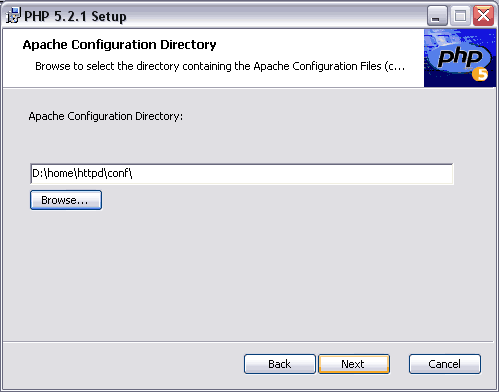
\includegraphics[scale=1,width=8cm]{ch01-05.png}
\caption{Вибір місцезнаходження файлу  <<httpd.conf>>}
\label{f1-5:image}
\end{figure}
Виберіть усі розширення PHP, що йдуть у комплекті, так ви не зіткнетесь з проблемами недостачі бібліотек під час навчання~(Рис.~\ref{f1-6:image}).

\begin{figure}
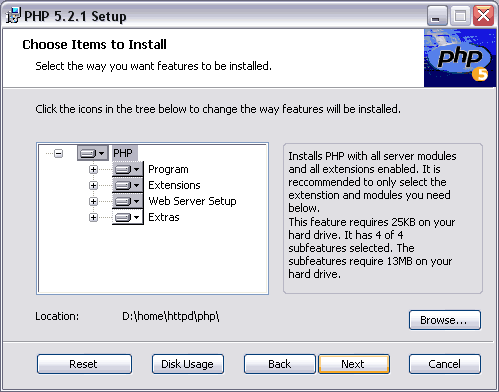
\includegraphics[scale=1,width=8cm]{ch01-06.png}
\caption{Вибір встановлюваних бібліотек}
\label{f1-6:image}
\end{figure}

У випадку проблеми прив'язки PHP до Apache його можна підключити безпосередньо у файлі <<httpd.conf>>. Для цього у файл необхідно додати такі рядки:

\begin{verbatim}
LoadModule php5_module c:/(каталог з PHP)/php5apache2_2.dll 
AddType application/x-httpd-php phtml php
PHPIniDir "c:/(каталог з PHP)/"
\end{verbatim}

Для перевірки роботи PHP та Apache створіть файл у каталозі вашого сайту <<phpinfo.php>> з такими рядками:
\pagebreak[3]
\penalty -20000
\begin{verbatim}
<?php
  echo phpinfo();
?> 
\end{verbatim}

В адресній строці браузера введіть \verb'http://localhost/phpinfo.php'. Якщо ви все виконали правильно, ви повинні побачити сторінку, зображену на Рис.~\ref{f1-7:image}:

\begin{figure}
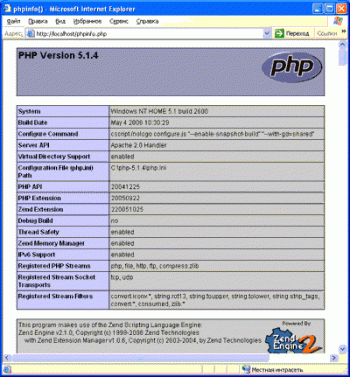
\includegraphics[scale=1,width=8cm]{ch01-07.png}
\caption{Результат роботи функції phpinfo()}
\label{f1-7:image}
\end{figure}

\pagebreak[3]

\section{Налаштування СКБД MySQL}
\nopagebreak[4]
При встановленні  СКБД MySQL вам необхідно запустити файл-інсталятор, даних за замовчуванням достатньо для встановлення повнофункціонального пакету. Після встановлення запуститься майстер налаштувань. Стандартних даних для роботи СКБД достатньо, одначе необхідно буде вказати пароль доступу адміністратора до СКБД в діалозі, зображеному на  Рис.~\ref{f1-8:image}.

\begin{figure}
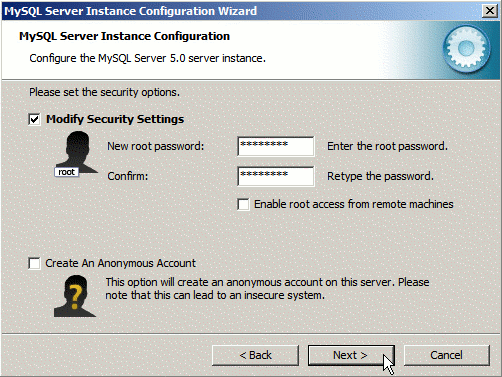
\includegraphics[scale=1,width=8cm]{ch01-08.png}
\caption{Введення пароля адміністратора СКБД}
\label{f1-8:image}
\end{figure}
Після встановлення пароля ви можете під'єднуватися до бази під логіном <<root>> та вказаним вами паролем.

\pagebreak[3]

\section{Індивідуальне завдання}
\nopagebreak[4]
\subsection*{Завдання до лабораторної роботи}
\nopagebreak[4]
\begin{enumerate}
\item Вивчити теоретичний матеріал
\item Відповісти на контрольні запитання
\item Скласти звіт
\item Захистити роботу
\end{enumerate}

\subsection*{Контрольні запитання}
\nopagebreak[4]
\begin{enumerate}
\item Що таке Internet? З яких структурних частин складається Internet?
\item Що таке IP-адреса?
\item Що таке доменне ім'я, з чого воно складається?
\item Який сервіс Internet перетворює IP-адреси в доменні імена і навпаки?
\item Яка служба займається розподіленням блоків IP-адрес?
\item Протокол HTTP. Рівень у моделі OSI, призначення.
\item Значення URI, URL, URN.
\item Мови web-програмування, які ви знаєте.
\item Веб-сервери, які ви знаєте.
\item Мережеві СКБД, які ви знаєте. 
\end{enumerate}




%\chapter{Форми HTML. Змінні, константи, масиви та функції в РНР}
\section*{Мета роботи}
Згадати основи мови розмітки веб-сторінок. Ознайомитись з базовими елементами мови РНР.
\nopagebreak[4]
\section{Формування HTML-сторінки засобами PHP}
\nopagebreak[4]
Код PHP зазвичай об'єднується з тегами XHTML. PHP є вбудовуваним мовою~--- це означає, що можна переміщатися між чистим кодом HTML і PHP, не жертвуючи можливістю читання тексту.
\index{PHP!теги відкриття/закриття}Щоб вбудувати код PHP в XHTML, PHP повинен задаватися відокремлено, за допомогою початкового та кінцевого тегів PHP. Теги PHP кажуть інтерпретатору, де починається і закінчується код PHP. Аналізатор PHP розпізнає три варіанти початкового і кінцевого тегів.

\begin{enumerate}



\item Перший варіант тегів PHP називається тегами в стилі XML і є кращим стилем. Він працює в документах розширювана мова розмітки (XML). Цей метод повинен використовуватися при з'єднанні PHP з документами XML і XHTML. Приклади в цьому підручнику застосовують цей формат тегів XML.

Стиль XML
\begin{verbatim}
<? PHP
//Блок коду PHP
>
\end{verbatim}

    
\item Скорочений стиль є найбільш простим, однак, він не рекомендується, тому що вступає в протиріччя зі стандартами документів XML та налаштуваннями в <<php.ini>>.

Скорочений стиль    
\begin{verbatim}
<?
//Блок коду PHP
>
\end{verbatim}

    
\item Цей стиль використовує найдовшу запис і схожий на стиль тегів, що застосовуються для включення кодів JavaScript. Цей стиль є кращим при використанні редактора HTML, який не розпізнає інші стилі тегів. Так як більшість нових редакторів XHTML розпізнають стиль тегів XML, то використання цього стилю не рекомендується.

Стиль сценарію
\begin{verbatim}
<script language="php">
//Блок коду PHP
</ SCRIPT>
\end{verbatim}
   
\end{enumerate}

PHP містить два основних оператора для виведення тексту в веб-браузері: \verb|echo| і  \verb|print|. Обидва оператора розміщуються між відкритим і закритим тегами блоку коду PHP і можуть перебувати в будь-якому місці в документах XHTML. Оператори  \verb|echo| і  \verb|print| використовують наступний формат:
\verb|echo|~--- використовується для виведення одного або кількох рядків.
\begin{verbatim}
echo "виведений текст";
\end{verbatim}
 \verb|print|~--- використовується для виведення рядка. В деяких випадках оператор  \verb|print| пропонує більшу функціональність, ніж оператор  \verb|echo|.
\begin{verbatim}
print "виведений текст";
\end{verbatim}
Наступні приклади демонструють використання і розміщення команд  \verb|echo| і  \verb|print| в документі XHTML.



\begin{lstlisting}[caption=Приклад вживання команд echo і print]
<!DOCTYPE html PUBLIC "-//W3C//DTD/XHTML 1.0 Transitional//EN"
  "http://www.w3.org/TR/xhtml1/DTD/xhtml11-transitional.dtd">
<html xmlns="http://www.w3.org/1999/xhtml" xml:lang="en" lang="en">
<head>
  <title> Страница Web </title>
</head>
<body>
<?php 
echo "Друк рядка оператором echo"."<br>";
print "Друк рядка оператором print";
?>
</body>
</html>
\end{lstlisting}



\pagebreak[3]
\section{Передача даних з HTML-форми PHP-сценарію}
\nopagebreak[4]
\index{HTML!передача данних}
Обробка форм є дуже важливою властивістю PHP. За допомогою форм користувачі взаємодіють зі сторінками Web, і з їхньою ж допомогою можна збирати інформацію для персоналізованих сторінок відвідувачів. У більш широкому сенсі інформаційної обробки, форми призначені для введення даних в системи обробки. Вони є первинним механізмом отримання даних, які обробляють сценарії для породження нової інформації, поновлення файлів і баз даних, а також для відповіді на запити користувачів для отримання інформації. Зовнішній вигляд типової форми дано на малюнку~\ref{f2-1:image}.

Передача даних з форм в РНР-сценарій відбувається методами  \verb|GET| або  \verb|POST| протоколу НТТР. Обидва методи однаково ефективні при використанні в формах з невеликою кількістю полів. Метод  \verb|POST| рекомендований при передачі великих обсягів тексту і файлів, обмеження за замовчуванням встановлено в 8 Мбайт і налаштовується у файлі  \verb|php.ini|.

Контейнер форми виглядає наступним чином:
\begin{verbatim}
<form name="form1" action="script.php" method="post">
</form>
\end{verbatim}
де \verb'name'~--- назва HTML-об'єкта, \verb'action' - відносний або абсолютний шлях до сценарію, якому передаються дані, \verb'method' - назва методу, яким передаються дані.

У контейнер форми поміщаються додаткові елементи управління, якими управляє користувач:

\subsection*{INPUT і його варіації}
\index{HTML!форми!input}
Елемент \verb'<input>' є найбільш вживаним тегом HTML-форм. За допомогою цього тега реалізуються основні функції форми. Він дозволяє створювати всередині форми поля введення рядка тексту, імені файлу, пароля і т.д. Також варто згадати про варіацію тега, що реалізує можливість завантаження файлів на сервер. Повний опис можливостей даного тега дано у додатку~\ref{inp-tag:app}
\subsection*{TEXTAREA}
\index{HTML!форми!textarea}
Елемент \verb'<textarea>' відповідає за передачу багаторядкового тексту. Важливо пам'ятати, що об'єм тексту, що передається обмежений параметрами методу, який використовується для передачі. Повний опис можливостей даного тега дано у додатку~\ref{tar-tag:app}
\subsection*{Списки вибору SELECT}
\index{HTML!форми!select}
Досить часто існує необхідність представити які-небудь дані у вигляді списку і передбачити можливість вибору в цьому списку. У HTML списки реалізуються за допомогою тега \verb'<select>'. Списки можуть давати можливість одиночного або множинного вибору. Повний опис можливостей даного тега дано у додатку~\ref{sel-tag:app}

\begin{figure}
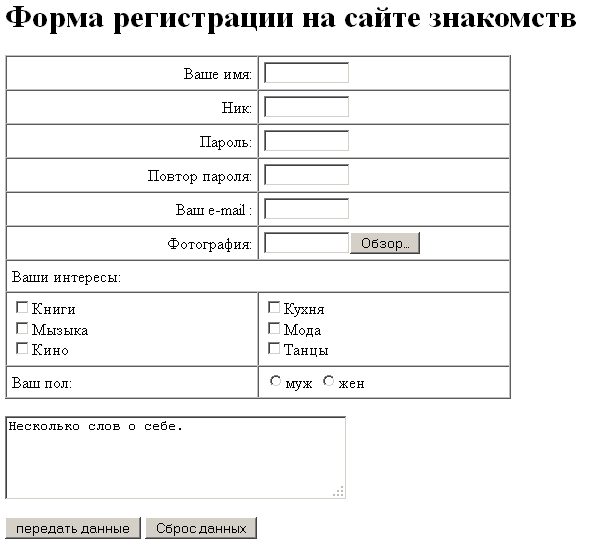
\includegraphics[scale=1,width=8cm]{ch02-01.png}
\caption{Вигляд HTML-форми}
\label{f2-1:image}
\end{figure}


\pagebreak[3]
\section{Змінні, константи та функції в РНР}
\nopagebreak[4]
\subsection*{Змінні}
\index{PHP!змінні}
\textbf{Змінні} є тимчасовим місцем зберігання, використовуваним для представлення значень в сценарії PHP. У PHP є два основні типи змінних: скалярні і масиви. Скалярні змінні містять тільки одне значення в даний момент часу, а змінні масиви - список значень. Змінні масиви обговорюються в наступному розділі. Скалярні змінні PHP містять значення типів описаних у лабораторній роботі №~\ref{datatypes}.

Імена змінних PHP всіх типів починаються зі знака <<\$>>. Імена змінних можуть містити літери, числа, і символ підкреслення (\_); вони не можуть, проте, починатися з цифри. У PHP імена змінних розрізняють регістр символів. 

\subsection*{Інтерполяція змінних}
\index{PHP!змінні!інтерполяція}
PHP підтримує також процес, званий інтерполяцією. \textbf{Інтерполяція}~--- заміна змінної в рядку її вмістом. Замість з'єднання змінних і літералів, їх можна об'єднувати всередині подвійних лапок (""). Змінні і літерали не можна об'єднати всередині одиночних лапок. При використанні подвійних лапок значення змінної виводиться разом з літералів. 
\begin{verbatim}
<?php 
$fname = "John";
$lname = "Doe";
echo "The user's name is $fname $lname";
?>
\end{verbatim}
\subsection*{Константи}
\index{PHP!константи}
\textbf{Константи}, як і змінні, є тимчасовим сховищем значень у пам'яті. На відміну від змінних значення константи ніколи не змінюється. При оголошенні константи використовується функція  \verb|define()|, яка вимагає задати ім'я константи і значення цієї константи.

Константам можна присвоювати такі типи даних.

Цілі~--- цілі числа або числа без десяткової крапки (1, 999, 325 812 841).

Числа з плаваючою точкою~--- числа, що містять десяткову крапку (1.11, 2.5, .44).

Рядки~--- текстова або числова інформація. Строкові дані завжди полягають в лапки ("Hello World", "478-477-5555").

Імена констант PHP на відміну від змінних не починаються зі знака <<\$>>. Імена констант звичайно записують у верхньому регістрі. Імена констант можуть містити літери, цифри та символ підкреслення (\_); вони не можуть, проте, починатися з цифри. Оголошення констант показано нижче.
\begin{verbatim}
define ("STRING_CONSTANT", "This is my string."); 
define ("NUMERIC_CONSTANT", 5); 
\end{verbatim}
Вивід констант подібний до виводу змінних.
\subsection*{Функції}
\index{PHP!функції}
\textbf{Функцією} називається фрагмент програмного коду, що володіє унікальним ім'ям і призначений для вирішення певного завдання. 

Функції використовуються для розбиття великих блоків коду на менші, більш керовані одиниці. Код, що міститься всередині функції, виконує певне завдання і повертає значення. PHP містить два типи функцій~--- визначені користувачем (або створені програмістом) і внутрішні (вбудовані функції), які є частиною визначення мови PHP.

Виклик вбудованої функції відбувається за допомогою її імені. Наприклад, функція, що виводить інформацію про РНР та Apache:
\begin{verbatim}
<?php
phpinfo();
?>
\end{verbatim}
У даному випадку функція викликається без параметрів. Наступна функція використовує ряд аргументів і повертає значення (у даному випадку дескриптор відкритого файлу:
\begin{verbatim}
<?php
f=fopen("d:\www\index.php","w+");
?>
\end{verbatim}
\pagebreak[3]
\section{Робота з масивами в РНР}
\nopagebreak[4]
\index{PHP!змінні!масиви}
Змінну масиву можна використовувати для зберігання множини або послідовності значень. Система PHP підтримує масиви з числовими індексами і асоціативні масиви. \textbf{Масив} в PHP є фактично впорядкованим відображенням. Відображення є типом, який відображає значення в ключі. Змінні масивів складаються з двох частин~--- індексу та елемента. Індекс масиву, іноді званий ключем масиву, є значенням, застосовуваним для ідентифікації або доступу до елементів масиву. Індекс масиву поміщається в квадратні дужки. Більшість масивів використовують числові індекси, які зазвичай починаються з 0 або 1. У PHP асоціативні масиви можуть використовувати рядкові індекси. Обидва типи масивів створюються за допомогою конструкції  \verb|array()|
\subsection*{Масиви з числовими індексами}
\begin{verbatim}
$my_array = array('red', 'green', 'blue'); 
\end{verbatim}
Цей код створює масив з числовим індексом з ім'ям \verb'$my_array'. Масиву присвоюється три елементи~---  \verb|red|,  \verb|green| і  \verb|blue|. Кожен елемент ідентифікується числовим індексом.
\begin{verbatim}
$my_array [0] = 'red' // індекс 0 відповідає елементу red 
$my_array [1] = 'green' // індекс 1 відповідає елементу green 
$my_array [2] = 'blue' // індекс 2 відповідає елементу blue 
\end{verbatim}
Щоб отримати доступ до вмісту масиву, використовується ім'я масиву та індекс. 
\subsection*{Асоціативні масиви}
Асоціативні масиви дозволяють використовувати більш корисні значення індексу. Для масивів з числовими індексами значення індексу створюються автоматично, починаючи з 0. Асоціативні масиви допускають застосування числових і строкових значень індексу.
\begin{verbatim}
$members = array('FName' => 'John', 'LName' => 'Smith', 'Age' => 50) 
\end{verbatim}
У цьому прикладі члени масиву містять три елементи, однак використовуються рядкові індекси~---  \verb|FName|,  \verb|LName| і  \verb|Age|.
\begin{verbatim}
$members ['FName'] = 'John' // індекс FName відповідає елементу John
$members ['LName'] = 'Smith' // індекс LName відповідає елементу Smith
$members ['Age'] = '50 '// індекс Age відповідає елементу 50 
\end{verbatim}
Для доступу до вмісту масиву використовується ім'я масиву та індекс.
\pagebreak[3]
\section{Функції, визначені користувачем}
\nopagebreak[4]
\index{PHP!функції!користувацькі функції}
\textbf{Визначені користувачем функції} створюються за допомогою ключового слова \verb'function'. Вони особливо корисні у великих програмах PHP, так як можуть містити блоки коду, які можуть використовуватися в програмі, що дозволяє уникнути повторного переписування коду. Далі представлений приклад простої визначеної користувачем функції PHP:
\begin{verbatim}
function AddNumbers ($num1, $num2)
{
echo "Це приклад функції PHP. 
Вона обчислює суму двох чисел і повертає 
результат програмі, що її викликала";
return $num1 + $num2;
} 
\end{verbatim}


Визначені користувачем функції можуть викликатися в будь-якому місці програми на PHP. У PHP функція виконується при використанні в коді її імені. Після виклику функція отримує всі передані їй значення у формі параметрів, виконує певні завдання і повертає значення програмі. 

\pagebreak[3]
\section{Змінні всередині функції}
\nopagebreak[4]
\index{PHP!змінні!локальні змінні}
\index{PHP!змінні!глобальні змінні}
\textbf{Глобальні змінні}~--- це змінні, які доступні всій програмі, включаючи підпрограми (користувальницькі функції).

\textbf{Локальні змінні}~--- змінні, визначені всередині підпрограми (користувацької функції). Вони доступні тільки всередині функції, в якій вони визначені.

Для PHP всі оголошені і використовувані у функції змінні за замовчуванням локальні для функції. Тобто, за умовчанням немає можливості змінити значення глобальної змінної в тілі функції. 

існує спеціальна інструкція \verb'global', що дозволяє функції користувача працювати з глобальними змінними. Розглянемо даний принцип на конкретному прикладі:

\begin{verbatim}
<?php
$a = 1 ;
$b = 2 ;

function sum()
{
global $a, $b;
$b = $a + $b;
}
?> 
\end{verbatim}

\pagebreak[3]
\section{Змінні-функції}
\nopagebreak[4]
\index{PHP!функції!змінні-функції}
PHP підтримує концепцію \textbf{змінних-функцій}. Це означає, що якщо до імені змінної приєднані круглі дужки, PHP шукає функцію з тим же ім'ям, що і результат обчислення змінної, і намагається її виконати. Цю можливість можна використовувати для реалізації зворотних викликів, таблиць функцій і безлічі інших речей.

Приклад використання змінної-функції наведено в додатку~\ref{var-func:app}

\pagebreak[3]
\section{Індивідуальне завдання}

\nopagebreak[4]
\subsection*{Завдання до лабораторної роботи}
\nopagebreak[4]
\begin{enumerate}
\item Вивчити теоретичний матеріал
\item Відповісти на контрольні запитання
\item Скласти алгоритм (блок-схему) програми
\item Виконати практичне завдання
\item Скласти звіт
\item Захистити роботу
\end{enumerate}

\subsection*{Контрольні запитання}
\nopagebreak[4]
\begin{enumerate}
\item Що таке змінні, константи та функції?
\item Що таке інтерполяція змінних?
\item Що таке масиви?
\item Як отримати доступ до індексного масиву? 
\item До ассоціативного?
\item Як створити користувацьку функцію?
\item Що таке локальні змінні?
\item Що таке глобальні змінні? Як ними користуватись у тілі функції?
\item Що таке змінні-функції?
\item Яким чином здійснюється виклик функції-змінної?
\end{enumerate}

\subsection*{Практичні завдання}
\nopagebreak[4]


\begin{enumerate}
\item[]Написати HTML-сторінку з формою, що складається з:
\item однорядкового поля вводу, поля вводу пароля та кнопки відправлення форми.
\item однорядкового поля вводу, прихованого текстового поля та кнопки відправлення форми.
\item однорядкового поля вводу, багаторядкового поля вводу та кнопки відправлення форми.
\item багаторядкового поля вводу, списку з одиночним вибором з п'яти елементів та кнопки відправлення форми.
\item прихованого текстового поля, списку з одиночним вибором з п'яти елементів та кнопки відправлення форми.
\item багаторядкового поля вводу, списку з множинним вибором з п'яти елементів та кнопки відправлення форми.
\item списку з одиночним вибором з п'яти елементів, поля вводу пароля та кнопки відправлення форми.
\item списку з множинним вибором з п'яти елементів, багаторядкового поля вводу та кнопки відправлення форми.
\item[]Отримати дані форми і вивести іх за допомогою функції в окремому сценарії.
\item створити асоціативний масив з днями тижня та вивести його на сторінку
\item створити індексний массив з назвами місяців і вивести його на екран
\item[]Написати HTML-сторінку з формою, що складається з однорядкового поля вводу та кнопки відправлення. Записати в поле число та обробити наступним чином:
\item створити константу та помножити на отримане з форми число 
\item створити змінну, занести в неї результат з форми, помножити змінну саму на себе
\item створити константу та обчислити вираз $x*const+2*x$
\item створити константу та обчислити вираз $\frac{x}{const}+x^2$
\item створити змінну та константу, в змінну занести константу і додати до числа з форми.
\item[]Результат вивести на сторінку 
\item[]Створити форму з трьома однорядковими полями і кнопкою відправлення форми
\item отримані з форми дані занести в асоціативний масив
\item отримані дані занести в індексний масив
\item[]зміст масиву роздрукувати функцією \verb'print_r()'; 
\item створити функцію, що друкує свій параметр
\item створити функцію, що перемножує два свої параметри і повертає результат. Результат роздрукувати
\item створити функцію, що перемножує свої параметри і друкує результат
\item створити функцію, що змінює глобальну змінну
\item створити функцію, що перемножує глобальну змінну і вхідний параметр, рузультат друкує
\item створити функцію, що домножує глобальну змінну на вхідний параметр і повертає результат
\item створити функцію, що формує індексний масив з двох локальних змінних і друкує його функцією \verb'print_r()';
\item створити функцію, що формує асоціативний масив з параметрів і друкує його функцією \verb'print_r()';

\end{enumerate}




%\chapter{Взаємодія PHP та web-сервера. Синтаксис PHP}
\nopagebreak[4]
\section*{Мета роботи}
Ознайомитись зі змінними оточення веб-серверу та суперглобальними масивами РНР. Ознайомитись з конструкціями розгалуження, циклів, включення файлів.
\section{Змінні оточення web-сервера Apache, суперглобальні масиви PHP}
\nopagebreak[4]

\subsection*{Змінні оточення web-сервера Apache}
\index{Web-сервери!Apache!змінні оточення}
\textbf{Змінні оточення}~--- дуже важливий механізм взаємодії веб-сервера з предобработчікамі запитів. При отриманні HTTP-запиту веб-сервер формує змінні оточення, заносячи в них різну інформацію: IP-адреса клієнта, запитуваний документ, параметри запиту і т.п. При передачі управління якомусь предобработчіку останній має доступ до змінних оточення веб-сервера, отже, йому доступна вище перерахована інформація.

Безпосередньо перед запуском сценарію сервер передає йому якісь змінні оточення з інформацією. Змінні оточення в мові PHP можна використовувати як звичайнісінькі змінні. Змінні оточення діляться на чотири великі групи:
\begin{enumerate}
\item Формовані сервером змінні;
\item Спеціальні змінні сервера Apache;
\item Змінні HTTP-полів запиту;
\item Змінні SSL-з'єднання (захищеного з'єднання).
\end{enumerate}

\subsection*{Суперглобальні масиви PHP}
\index{PHP!змінні!суперглобальні масиви}
\textbf{Суперглобальними масивами} (superglobal arrays) в PHP називаються зумовлені масиви, які видно в будь-якому місці вихідного коду без використання ключового слова \verb'global'.


Доступ до змінних оточення здійснюється через суперглобальний масив \verb'$_SERVER' у вигляді \verb|$_SERVER['змінна_CGI']|; Наприклад код
\begin{verbatim}
print $_SERVER['SERVER_SOFTWARE'];
\end{verbatim}
роздрукує в браузері строку виду:
\begin{verbatim}
Apache/2.2.4 (Win32) mod_ssl/2.2.4 OpenSSL/0.9.8k PHP/5.3.3
\end{verbatim}


Повний перелік змінних оточення web-сервера Apache та суперглабальних масивів PHP дивіться у додатках~\ref{var-apa:app} та~\ref{sup-glob:app}.


\pagebreak[3]



\section{Оператори PHP}
\nopagebreak[4]
\index{PHP!оператори}
Синтаксис PHP дуже нагадує синтаксис мови C і багато в чому запозичений з таких мов як Java і Perl. Інструкції поділяються також як і в C або Perl~--- кожен вираз закінчується крапкою з комою. Закриваючий тег <<?> >> також має на увазі кінець інструкції.

Коментарі застосовуються в PHP для запису власних зауважень під час процесу розробки коду. Такі коментарі можуть визначати призначення сегмента коду або їх можна використовувати для виключення блоків коду під час тестування і налагодження сценаріїв.

Синтаксичний аналізатор PHP ігнорує коментарі. Коментарі в PHP можна визначити одним з наступних способів:
\begin{enumerate}

\item \verb|//|~--- Простий коментар PHP;
\item \verb|#|~--- Альтернативний простий коментар PHP;
\item \verb|/* ... */|~--- Багаторядкові блоки коментарів.

\end{enumerate}
\penalty -10000
Імена змінних позначаються знаком \$.

\begin{verbatim}
<?php
$message = "Привет, я - скрипт PHP!";
echo $message;
?>
\end{verbatim}
\index{PHP!змінні!типи даних}
PHP підтримує вісім простих типів даних \label{datatypes}:
\begin{enumerate}
\item Чотири скалярних типи:
		\begin{itemize}
		\item Boolean (двійкові дані)
		\item Integer (цілі числа)
		\item Float (числа з плаваючою точкою або 'double')
		\item String (рядки)
		\end{itemize}
\item Два змішаних типи:
		\begin{itemize}
		\item Array (масиви)
		\item Object (об'єкти)
		\end{itemize}
\item Два спеціальних типи:
		\begin{itemize}
		\item resource (ресурси)
		\item NULL (<<порожні>>)
		\end{itemize}
\item Існують також кілька псевдотіпов:
		\begin{itemize}
		\item Mixed (змішані)
		\item Number (числа)
		\item Callback (зворотний визов)		
		\end{itemize}
\end{enumerate}

Основними конструкціями мови PHP є:
\index{PHP!конструкції}
\begin{enumerate}
\item Умовні оператори (\verb|if, else|);
\item Цикли (\verb|while, do-while, for, foreach, break, continue|);
\item Конструкції вибору (\verb|switch|);
\item Конструкції оголошення (\verb|declare|);
\item Конструкції повернення значень (\verb|return|);
\item Конструкції включень (\verb|require, include|).
\end{enumerate}


Для здійснення операцій зі змінними існують різні групи операторів. Оператором називається дещо, що складається з одного або більше значень (виразів), яке можна обчислити як нове значення (таким чином, вся конструкція може розглядатися як вираз).

\textbf{Оператори бувають трьох видів.}
\begin{enumerate}
\item Унарні оператори, які працюють тільки з одним аргументом, наприклад, <<!>> (оператор заперечення) або <<++>> (інкрімент).
\item Бінарні оператори: до них належать більшість підтримуваних в PHP операторів
\item тернарних оператор <<\dots?\dots:\dots>>. Він використовується для умовного вибору між двома операторами, в залежності від результату обчислення третього оператора.
\end{enumerate}
\subsection*{Пріоритет виконання операторів}
\index{PHP!оператори!пріоритети}
Пріоритет операторів визначає, в якому порядку будуть обчислюватися два і більше вирази. Наприклад, вираз $1 + 5 * 3$ обчислюється як 16, а не 18, оскільки операція множення <<*>> має більш високий пріоритет, ніж операція додавання <<+>>. У разі, якщо оператори мають однаковий пріоритет, вони будуть виконуватися зліва направо. Круглі дужки можуть використовуватися для примусового вказівки необхідного порядку виконання операторів. Наприклад, вираз $(1 + 5) * 3$ обчислюється як 18.

В таблиці~\ref{pr-op:table} додатку надано пріоритети виконання операторів PHP.

Ліва асоціативність вказує на те, що вираз обчислюється зліва направо, права асоціативність відповідно має увазі протилежний порядок.
\pagebreak[3]
\section{Конструкції вибору}
\index{PHP!конструкції!розгалуження}
\nopagebreak[4]
До конструкцій вибору відносять: умовний оператор (\verb'if...else') і перемикач (\verb'switch'). 
\subsection*{if \dots else}
Синтаксис умовного оператора:
\begin{verbatim}
if (condition) statement1 else statement2
\end{verbatim}


Умова \verb'condition' може бути будь-яким виразом. Якщо \verb'condition' істинне, то виконується оператор \verb'statement1' . В іншому випадку виконується оператор \verb'statement' 2. Допустима скорочена форма запису умовного оператора, в якій відсутні \verb'else' і оператор \verb'statement2'.

У свою чергу, оператори \verb'statement1' і \verb'statement2' можуть бути умовними, що дозволяє організовувати послідовність перевірок будь-якої глибини вкладеності. І в цих послідовностях кожен умовний оператор може бути як повним, так і скороченим. У зв'язку з цим можливі помилки неоднозначного зіставлення \verb'if' і \verb'else'.

Зауважимо, що перевірка додаткових умов можлива за допомогою оператора \verb|elseif|. Оператор \verb|if| може включати скільки завгодно блоків \verb'elseif', але else в кожному if може бути тільки один. Як правило, в конструкціях \verb'if ... elseif ... else' оператор else визначає, що потрібно робити, якщо ніякі інші умови не є true. 

РНР надає також можливість альтернативного синтаксису умовного оператора~--- без фігурних дужок, а із застосуванням оператора \verb'endif', при цьому оператори будуть розміщені всередині блока.

\subsection*{Перемикач <<switch>>}

Перемикач \verb'switch' є найбільш зручним засобом для організації множинного розгалуження. Синтаксис перемикача такий:
\penalty -10000
\begin{verbatim}
switch (expression) 
{
case value1: statements; break;
case value2: statements; break;
default:
statements;
}
\end{verbatim}

Керуюча структура \verb'switch' передає керування тому з помічених \verb'case' операторів, для якого значення константного виразу збігається зі значенням \verb'expression'. Якщо значення \verb'expression' не збігається ні з одним з константних виразів, то виконується перехід до оператора, поміченого міткою \verb'default'. У кожному перемикачі може бути не більше однієї мітки \verb'default', однак вона може бути відсутньою взагалі.


\pagebreak[3]

\section{Конструкції циклів}
\nopagebreak[4]

\index{PHP!конструкції!цикли}

На другому місці за частотою використання, після конструкцій умов (умовних операторів), знаходяться цикли.

Цикли дозволяють повторювати певну (і навіть невизначений~--- коли робота циклу залежить від умови) кількість разів різні послідовності операторів. Дані оператори називаються тілом циклу. Прохід циклу називається ітерацією.

PHP підтримує чотири види циклів:
\begin{itemize}
\item    Цикл з передумовою (while)
\item    Цикл з постусловіем (do-while)
\item    Цикл з лічильником (for)
\item    Спеціальний цикл перебору масивів (foreach)
\end{itemize}

Цикли зручно також використовувати при форматуванні HTML-сторінки. Наприклад при створенні великих списків або таблиць.

\begin{lstlisting}[caption=Формування HTML-сторінки за допомогою циклів]
<!DOCTYPE html PUBLIC "-//W3C//DTD/XHTML 1.0 Transitional//EN"
  "http://www.w3.org/TR/xhtml1/DTD/xhtml11-transitional.dtd">
<html xmlns="http://www.w3.org/1999/xhtml" xml:lang="en" lang="en">
<head>
  <title> Страница Web </title>
</head>
<body>
<table>
<?php
for (int $i=1; $i<=10; $i++) 
echo "<tr><td> Рядок № </td><td>$i</td></tr>\n";
?>
</table>
</body>
</html>
\end{lstlisting}




Сценарій для тієї самої сторінки без використання циклів зайняв б у два рази більше дискового простору.

При використанні циклів є можливість використання операторів \verb'break' і \verb'continue'. Перший з них перериває роботу всього циклу, а другий~--- тільки поточної ітерації.


\subsection*{Цикл з передумовою while}
\index{PHP!конструкції!while}
Цикл з передумовою while працює за такими принципами:

\begin{enumerate}
\item    Обчислюється значення логічного виразу.
\item    Якщо значення істинно, виконується тіло циклу, в іншому випадку~--- переходимо на наступний за циклом оператор.
\end{enumerate}


Синтаксис циклу з передумовою:
\begin{verbatim}
while (логічний_вираз) інструкція;
\end{verbatim}

В даному випадку тілом циклу є інструкція. Зазвичай тіло циклу складається з великої кількості операторів. Наведемо приклад циклу з передумовою while:
\begin{verbatim}
<? Php
$х = 0;
while ($x++<10) echo $x;
// Виводить 12345678910
?>
\end{verbatim}
Зверніть увагу на послідовність виконання операцій умови \$x++<10. Спочатку перевіряється умова, а тільки потім збільшується значення змінної. Якщо ми поставимо операцію інкремента перед змінної (++\$x<10), то спочатку буде виконано збільшення змінної, а тільки потім~--- порівняння. У результаті ми отримаємо рядок <<123456789>>. 


Подібно конструкції умовного оператора \verb'if', можна групувати оператори всередині тіла циклу while, використовуючи наступний альтернативний синтаксис:
\begin{verbatim}
while (логічний_вираз):
інструкція;
...
endwhile;
\end{verbatim}

\subsection*{Цикл з постумовою do while}
\index{PHP!конструкції!do while}
На відміну від циклу \verb'while', цей цикл перевіряє значення виразу не до, а після кожного проходу (ітерації). Таким чином, тіло циклу виконується хоча б один раз. Синтаксис циклу з постумовою такий:
\begin{verbatim}
do
{
тело_цікла;
}
while (логічний_вираз);
\end{verbatim}
Після чергової ітерації перевіряється, чи істинний \verb'логічний_вираз', і, якщо це так, управління передається знову на початок циклу, в іншому випадку цикл обривається.

\subsection*{Цикл з лічильником <<for>> (регулярний цикл)}
\index{PHP!конструкції!for}
Цикл з лічильником використовується для виконання тіла циклу певне число разів. 

Синтаксис циклу \verb'for' такий:
\begin{verbatim}
for (ініціалізуючі_команди; умова_роботи; 
	команди_після_ітерації) {тіло_цикла;}
\end{verbatim}
Цикл for починає свою роботу з виконання \verb'ініціалізуючіх_команди'. Дані команди виконуються тільки один раз. Після цього перевіряється \verb'умова_роботи', якщо воно істинно (true), то виконується \verb'тіло_цикла'. Після того, як буде виконаний останній оператор тіла, виконуються \verb'команди_після_ітерації'.



Для циклу for є і альтернативний синтаксис:
\begin{verbatim}
for (ініціалізуючі_команди; умова_роботи; 
команди_після_ітерації):
оператори;
endfor;
\end{verbatim}

\subsection*{Цикл перебору масивів <<foreach>>}
\index{PHP!конструкції!foreach}
В PHP4 з'явився ще один спеціальний тип циклу~--- \verb'foreach'. Даний цикл призначений спеціально для перебору масивів.

Синтаксис циклу \verb'foreach' виглядає наступним чином:
\begin{verbatim}
foreach (масив as $ключ => $значення)
команди;
\end{verbatim}
Тут команди циклічно виконуються для кожного елемента масиву, при цьому чергова пара <<ключ => значення>> виявляється в змінних \verb'$ключ' і \verb'$значення'. 

У циклу foreach є й інша форма запису, яку слід застосовувати, коли нас не цікавить значення ключа чергового елемента. Виглядає вона так:
\begin{verbatim}
foreach (масив as $значення)
команди;
\end{verbatim}
У цьому випадку доступно лише значення чергового елементу масиву, але не його ключ. Це може бути корисно, наприклад, для роботи з масивами-списками:



Увага: Цикл \verb'foreach' оперує не вихідним масивом, а його копією. Це означає, що будь-які зміни, які вносяться в масив, не можуть бути <<видимі>> з тіла циклу. Що дозволяє, наприклад, в якості масиву використовувати не тільки змінну, але і результат роботи якої-небудь функції, що повертає масив (у цьому випадку функція буде викликана всього один раз~--- до початку циклу, а потім робота буде проводитися з копією повернутого значення).

\subsection*{Конструкція <<break>>}
\index{PHP!конструкції!break}
Дуже часто для того, щоб спростити логіку якого-небудь складного циклу, зручно мати можливість його перервати в ході чергової ітерації (наприклад, при виконанні якого-небудь особливого умови). Для цього і існує конструкція break, яка здійснює негайний вихід з циклу. Вона може задаватися з одним необов'язковим параметром~--- числом, яке вказує, з якого вкладеного циклу має бути здійснений вихід. За замовчуванням використовується 1, тобто вихід з поточного циклу, але іноді застосовуються й інші значення. Синтаксис конструкції \verb'break':
\begin{verbatim}
break; // За замовчуванням
break (номер_цикла); // Для вкладених циклів 
(вказується номер циклу, що переривається)
\end{verbatim}

\subsection*{Конструкція <<continue>>}
\index{PHP!конструкції!continue}
Конструкція \verb'continue' так само, як і \verb'break', працює тільки <<в парі>> з циклічними конструкціями. Вона негайно завершує поточну ітерацію циклу та переходить до нової (звичайно, якщо виконується умова циклу для циклу з передумовою). Точно так само, як і для \verb'break', для continue можна вказати рівень вкладеності циклу, який буде продовжений з повернення управління.


\pagebreak[3]

\section{Конструкції включення}
\nopagebreak[4]
Конструкції включень дозволяють збирати PHP програму (скрипт) з декількох окремих файлів.

У PHP існують дві основні конструкції включень: \verb'require' і \verb'include'.
\subsection*{Конструкція включень <<require>>}
\index{PHP!конструкції!require}
Конструкція \verb'require' дозволяє включати файли в сценарій PHP до виконання сценарію PHP. Загальний синтаксис \verb'require' такий:
\begin{verbatim}
require им'я_файлу;
або
require (им'я_файлу);
\end{verbatim}
При запуску (саме при запуску, а не при виконанні!) Програми інтерпретатор просто замінить інструкцію на вміст файлу \verb|им'я_файлу| (цей файл може також містити сценарій на PHP, обрамлений, як зазвичай, тегами << <? >> та << ?> >>'). Причому зробить він це безпосередньо перед запуском програми (на відміну від include , який розглядається нижче). Це буває досить зручно для включення в висновок сценарію різних шаблонних сторінок HTML-кодом. 
\subsection*{Конструкція <<include>>}
\index{PHP!конструкції!include}
Конструкція \verb'include' також призначена для включення файлів в код сценарію PHP.

На відміну від конструкції \verb'require' конструкція \verb'include' дозволяє включати файли в код PHP скрипта під час виконання сценарію. Синтаксис конструкції \verb'include' виглядає наступним чином:
\penalty -10000
\begin{verbatim}
include им'я_файлу;
або
include (им'я_файлу);
\end{verbatim}

Принципова різниця між цими двома операторами в тому, що \verb'include' дозволяє включати файли <<на літу>>, і робити це декілька разів, наприклад у циклах.
\subsection*{Конструкції одноразового включення <<require\_once>> і <<include\_once>>}
\index{PHP!конструкції!require\_once} \index{PHP!конструкції!include\_once}
У великих PHP сценаріях інструкції \verb'include' і \verb'require' застосовуються дуже часто. Тому стає досить складно контролювати, як би випадково не включити один і той же файл декілька разів, що найчастіше призводить до помилки, яку складно виявити.

У PHP передбачено вирішення даної проблеми. Використовуючи конструкції одноразового включення \verb'require_once' і \verb'include_once', можна бути впевненим, що один файл не буде включено двічі. Працюють конструкції одноразового включення \verb'require_once' і \verb'include_once' так само, як і \verb'require' і \verb'include' відповідно. Різниця в їх роботі лише в тому, що перед включенням файлу інтерпрететор перевіряє, чи включений вказаний файл раніше чи ні. Якщо так, то файл не буде включено знову. 

\subsection*{Включення віддалених файлів}

Конструкції однократних включень \verb'require_once' і \verb'include_ince' також дозволяють включати віддалені файли, якщо така можливість включена в конфігураційному файлі PHP.

Якщо \verb'URL fopen' увімкнено в PHP (як у конфігурації за замовчуванням), ви можете специфікувати файл, що підключається з використанням URL (через HTTP), замість локального шляху. 

Для того, щоб віддалене включення файлів було доступно, необхідно в конфігураційному файлі (php.ini) встановити \verb'allow_url_fopen = 1'.


\pagebreak[3]

\section{Конструкція <<or exit()>> (<<or die()>>)}
Конструкція складається з логічного оператора \verb'or' та функції \verb'exit()' або її псевдоніма \verb'die()'. Функція \verb'exit(статус)' друкує на екрані статус, котрий може бути цілочисельною або рядковою константою. Конструкцію зручно використовувати під час налагодження сценаріїв у комбінації з функціями, які можуть повертати логічне \verb'FALSE'. Наприклад зупинку сценарію при невдалому відкритті файлу можна отримати таким чином:
\begin{verbatim}
$file = fopen("file.txt","w+") or die("Помилка відкриття файлу");
\end{verbatim} 



\pagebreak[3]

\section{Індивідуальне завдання}

\nopagebreak[4]
\subsection*{Завдання до лабораторної роботи}
\nopagebreak[4]
\begin{enumerate}
\item Вивчити теоретичний матеріал
\item Відповісти на контрольні запитання
\item Скласти алгоритм (блок-схему) програми
\item Виконати практичне завдання
\item Скласти звіт
\item Захистити роботу
\end{enumerate}

\subsection*{Контрольні запитання}
\nopagebreak[4]
\begin{enumerate}
\item Які оператори виводу тексту ви знаєте?
\item Які групи змінних оточення ви знаєте?
\item Що таке суперглобальні масиви, як ними користуватись?
\item Яким чином можна задати коментар?
\item Які типи операторів ви знаєте?
\item Які конструкції вибору ви знаєте?
\item Які конструкції циклів ви знаєте?
\item У якому випадку цикл виконується хоча-б один раз?
\item Якими чином можна включити інший текстовий файл у сценарій?
\item Яка особливість операторів <<include\_once>> та <<require\_once>>? 
\end{enumerate}

\subsection*{Практичні завдання}
\nopagebreak[4]


\begin{enumerate}
 
\item[]Створити окремий РНР-файл, підключити його у головну сторінку. Файл повинен:
\item У регулярному циклі виводити числа від 1 до 20
\item У циклі з передумовою виводити числа від 20 до 50
\item У циклі з постумовою вивести числа від -50 до -10
\item Використовуючи регулярний цикл вивести елементи арифметичної прогресії з 20 елементів починаючи з 1 та доданком 2
\item Використовуючи з передумовою вивести елементи геометричної прогресії з 20 елементів починаючи з 1 та доданком 2
\item Розрахувати факторіал 10 за допомогою регулярного циклу
\item Вивести латинський алфавіт, використовуючи регулярний цикл
\item Вивести латинський алфавіт, використовуючи цикл з передумовою
\item Вивести Цифри від 20 до 0 у зворотньому порядку, використовуючи цикл з постумовою.
\item[]Написати HTML-сторінку з формою, що складається з однорядкового поля вводу та кнопки відправлення форми. В поле вводу ввести число та обчислити вираз: 
\item якщо $x>0$ то $5*x^2 + 2*x - 10$, інакше $5*x^2 + 2*x + 10$
\item якщо $0<x\le 10$ то $10*x^3 - 2*x - 10$, інакше $x^2 + 20*x$
\item якщо $0<x\le 20$ то $\frac{x}{x+1} + 2*x - 10$, інакше $\frac{x+1}{x} + 10$
\item якщо $-10<x\le 0$ то $5*x^2 + 2*x - 10$, $x> 0$ $5*x^2 + 2*x + 10$, інакше $\frac{x+1}{x} + 10$
\item якщо $x\le 10$ то $x^3 + 2*x^2$, інакше $2*x + 10$
\item якщо $x>10$ то $5*x^2 + \frac{x}{2}$, інакше $\frac{x+10}{x+1}$
\item[]Написати HTML-сторінку з формою, що складається з однорядкового поля вводу та кнопки відправлення форми. В поле вводу ввести число та використовуючи конструкцію <<switch-case>>: 
\item за номером дня тижня вивести його назву.
\item за номером місяця року вивести його назву.
\item від 0 до 10 вивести назви цифр
\item відповідно номера вивести букву латинського алфавіту
\item[]Опрацювати змінні оточення 
\item вивести шлях до каталогу з веб-документами
\item вивести підпис веб-сервера
\item вивести інформацію про браузер користувача
\item вивести адресу електронної пошти адміністратора
\item за допомогою конструкції перебору масивів вивести зміст \$\_SERVER
\item за допомогою конструкції перебору масивів вивести зміст \$\_ENV

\end{enumerate}

%\chapter{Робота з рядками. Регулярні вирази}
\section*{Мета роботи}
Ознайомитись із засобами роботи з рядковими змінними та константами. Ознайомитись із застосуванням регулярних виразів у мові РНР та SQL-запитах.
\nopagebreak[4]
\section{Рядки. Функції роботи з рядками}
\nopagebreak[4]
\index{PHP!змінні!рядки}
\textbf{Рядки є послідовностями символів}. У PHP символ відповідає байту, тобто існує точно 256 можливих різних символів. Рядки можуть бути дуже великими. У PHP не існує практичного обмеження на розмір рядків, тому взагалі немає причин турбуватися про їх довжині. Строкові значення можуть використовуватися буквально або присвоюватися змінним.

У PHP рядковий літерал можна задати трьома способами.
\begin{itemize}
\item рядки в одиночних лапках
\item рядки в подвійних лапках
\item рядки в синтаксисі heredoc 
\end{itemize}

\subsection*{Рядки в одиночних лапках}
Одиночні лапки надають найпростіший метод для роботи з рядками. При використанні цього методу рядки укладаються в одиночні лапки <<''>>. Якщо одиночні лапки потрібні як частина рядка, вони повинні бути екрановані символом зворотної косої межі <<\\>>. Хоча одиночні лапки надають простий спосіб роботи з рядками, одиночні лапки не підтримують застосування інтерполяції.
\subsection*{Рядки в подвійних лапках}
Рядки PHP можна виводити також за допомогою подвійних лапок <<"">>. Якщо рядки PHP поміщаються в подвійні лапки, то можна застосовувати інтерполяцію. Для рядків у подвійних лапках PHP підтримує також більшість екранованих символів. Ці символи представлені в таблиці~\ref{doub-lap:table} нижче.

\begin{center}
\begin{longtable}[t]{|l|p{20em}|}
\caption{Екрановані символи у подвійних лапках} \label{doub-lap:table}\\
\hline
Символ & Опис \\
\hline
\verb'\N' & перенесення рядка \\
\verb'\R' & повернення каретки \\
\verb'\T' & горизонтальна табуляція \\
\verb'\\' & зворотна коса риска \\
\verb'\$' & знак долара \\
\verb'\"' & подвійні лапки \\
\hline
\end{longtable}
\end{center}

\subsection*{Рядки в синтаксисі heredoc}
\textbf{Heredoc}-синтаксис~--- спосіб визначення строкових змінних у вихідному коді програм.

При визначенні строкових змінних їх вміст, зазвичай, полягає в одинарні або подвійні лапки, у зв'язку з чим символи лапок, які повинні бути частиною даних, доводиться екранувати за допомогою escape-послідовностей. Heredoc-синтаксис дозволяє визначити рядок, не укладаючи її в лапки, у зв'язку з чим необхідність екранування цих символів відпадає.

Приклад використання такого синтаксису наведено нижче:
\begin{verbatim}
$S = << EOL; 
Лапки бувають 'одинарними' і "подвійними". 
EOL
\end{verbatim} 
\subsection*{Функції роботи з рядками}
\index{PHP!змінні!рядки!функції}
У базовому наборі РНР існує величезна кількість функцій для обробки рядків. Як правило іх достатньо для написання програм, іноді необхідно комбінувати ці функції між собою для отримання необхідного результату. Повний перелік функцій дан у таблиці~\ref{str-func:table} додатків.

\pagebreak[3]
\section{Рядки, що включають HTML-код}
\nopagebreak[4]

\index{PHP!змінні!HTML-рядки}Досить часто ми працюємо з рядками, що містять html-теги. Якщо відобразити такий рядок в браузері за допомогою звичайних функцій відображення даних \verb'echo()' або \verb'print()', то ми не побачимо самих html-тегів, а отримаємо відформатовану у відповідності з цими тегами сторінку. Браузер обробляє всі html-теги у відповідності зі стандартом мови HTML. Іноді нам потрібно бачити безпосередньо рядок, без обробки його браузером. Щоб цього досягти, потрібно перед тим, як виводити, застосувати до рядка функцію \verb'htmlspecialchars()'.

\pagebreak[3]
\section{Регулярні вирази}
\nopagebreak[4]
\index{PHP!регулярні вирази}
\textbf{Регулярний вираз} (regular expression)~--- це технологія, яка дозволяє задати шаблон і здійснити пошук даних, відповідних цьому шаблону, в заданому тексті, представленому у вигляді рядка. Одне з поширених застосувань регулярних виразів~--- це перевірка рядка на відповідність будь-яким правилам.

Приклад регулярного виразу:
\begin{verbatim}
/^\w+([\.\w]+)*\w@\w((\.\w)*\w+)*\.\w{2,3}$/
\end{verbatim}
Основна перевага РВ полягає в тому, що вони дозволяють організувати більш гнучкий пошук, тобто знайти те, про що немає точного знання, але є приблизне уявлення. Наприклад, потрібно знайти всі семизначні номери телефонів, що зустрічаються в тексті. Ми не шукаємо якийсь заздалегідь відомий нам номер телефону, ми знаємо тільки, що шуканий номер складається з семи цифр. Для цього можна скористатися наступним РВ:

\begin{verbatim}
/\d{3}-\d{2}-\d{2}/m
\end{verbatim}

Одним з основних метасимволів є зворотний слеш <<\\>>. Він змінює тип символу, наступного за ним, на протилежний, тобто якщо це був звичайний символ, то він МОЖЕ перетворитися в метасимвол, якщо це був метасимвол, то він втрачає своє спеціальне значення і стає звичайним символом (це потрібно для того, щоб вставляти в текст спеціальні символи як звичайні). Наприклад, символ <<d>> в звичайному режимі не має ніяких спеціальних значень, але <<\\d>> є метасимволом, що означає "будь-яка цифра". Символ <<.>> в звичайному режимі означає будь одиничний символ, а <<\\.>> означає просто крапку.

Результати використання зворотнього слеша надано у таблиці\index{PHP!регулярні вирази!слеш-комбінації}:
\begin{center}
\begin{longtable}[t]{|l|p{20em}|}
\kill
\caption{\space Використання зворотнього слеша у регулярних виразах} \label{chr-meta:table}\\
\hline

Символ & Значення \\
\hline \endfirsthead
\caption*{\space Продовження} \\
\hline
Символ & Значення \\
\hline \endhead
\hline \endfoot
\verb'\n' & cимвол перекладу рядка \\

\verb'\e' & символ escape \\

\verb'\t' & cимвол табуляції \\

\verb'\Xhh' & символ в шістнадцятковому коді, наприклад \verb'\x41' є буква A і т.д. \\

\verb'\d' & будь-яка десяткова цифра (0-9) \\

\verb'\D' & будь-який символ, який не є десятковим цифрою \\

\verb'\s' & будь-який порожній символ (пробіл або табуляція) \\

\verb'\S' & будь-який символ, який не є порожнім \\

\verb'\w' & символ, використовуваний для написання Perl-слів (це літери, цифри та символ підкреслення), так званий "словниковий символ" \\

\verb'\W' & знайдене символ (всі символи, крім обумовлених \verb'\w') \\ 
\hline
\end{longtable}
\end{center}

Приклад використання наведених вище метасимволів:

\begin{verbatim}
/\d\d\d plus \d is \w\w\w/
\end{verbatim}

Цей регулярний вираз означає: тризначне число, за яким слідує підрядок \verb'plus', будь-яка цифра, потім \verb'is' і слово з трьох словникових символів. Зокрема, даним РВ задовольняють рядки: <<\verb'123 plus 3 is sum'>>, <<\verb'213 plus 4 is 217'>>.

\pagebreak[3]
\section{Функції PHP для роботи з регулярними виразами}
\nopagebreak[4]
\index{PHP!регулярні вирази!функції}
Основні функції для роботи з Perl-сумісними регулярними виразами: \verb'preg_match(pattern, string, [result, flags])' і \verb'preg_match_all(pattern, string, result, [flags])', де:

\verb'pattern'~--- шаблон регулярного виразу;

\verb'string'~--- рядок, в якій проводиться пошук;

\verb'result'~--- містить масив результатів (нульовий елемент масиву містить відповідність всьому шаблоном, перший~--- першому <<захопленому>> підшаблону і т.д.);

\verb'flags'~--- необов'язковий параметр, що визначає те, як впорядковані результати пошуку.

Ці функції здійснюють пошук за шаблоном і повертають інформацію про те, скільки разів відбувся збіг. Для \verb'preg_match()' це O (немає збігів) або 1, оскільки пошук припиняється, як тільки знайдено перший збіг. Функція \verb'preg_match_all()' робить пошук до кінця рядка і тому знаходить всі збіги. Всі точні збіги містяться в першому елементі масиву result у кожної з цих функцій (для \verb'preg_match_all()' цей елемент~--- теж масив). 
Аналогом \verb'preg_match' є булева функція POSIX-розширення \verb'ereg(string pattern, string string [, array regs])'

Функція \verb'ereg()' повертає \verb'TRUE', якщо збіг знайдено, і \verb'FALSE'~--- у противному випадку.

Наведені далі приклади можна тестувати на перерахованих функціях. Наприклад, так:



\begin{lstlisting}[caption=Приклад роботи з регулярними виразами]
<?
//Рядок, в якому потрібно щось знайти
$str = "Мій телефонний номер:".
"33-22-44. Номер мого редактора:".
"222-44-55 та 323-22-33";
//Шаблон, по якому шукати.
//Задає пошук семизначних номерів.
$pattern = "/\d{3}-\d{2}-\d{2}/m";
//Функція, що здійснює пошук
$num_match = preg_match_all($pattern, $str, $result);
//Вивід результатів пошуку
for ($i = 0; $i <$num_match; $i++) 
echo "Збіг $i:".$result[0][$i]."<br>";
?>
\end{lstlisting}






\pagebreak[3]
\section{Регулярні вирази в SQL-запитах}
\nopagebreak[4]
\index{MySQL!SQL!регулярні вирази}
Більшість сучасних СУБД також підтримують регулярні вирази. Це буває корисним коли необхідно отримати або змінити дані в базі, що відповідають певному шаблону.

В MySQL використовується розширена версія  реалізації регулярних виразів, яка орієнтована на відповідність POSIX 1003.2. Це розширена версія, в якій підтримуються операції порівняння із зразком, використовуючи оператор \verb'REGEXP' в операторах SQL.

Наприклад запит \verb|SELECT * FROM tab WHERE text REGEXP "B[an]*s"| поверне рядки <<Bananas>> та <<Baaaaas>>, якщо такі є в таблиці бази даних.

Перелік метасимволів, що підтримує MySQL, дано в таблиці~\ref{chr-rxp:table} додатків.

Альтернативою \verb'REGEXP' може виступати оператор \verb'RLIKE'. Оператор \verb'RLIKE' можна використовувати з запереченням \verb'NOT RLIKE'~--- в цьому випадку результатом його роботи буде вибірка рядків не відповідають заданим параметрам.
\pagebreak[3]
\section{Індивідуальне завдання}

\nopagebreak[4]
\subsection*{Завдання до лабораторної роботи}
\nopagebreak[4]
\begin{enumerate}
\item Вивчити теоретичний матеріал
\item Відповісти на контрольні запитання
\item Скласти алгоритм (блок-схему) програми
\item Виконати практичне завдання
\item Скласти звіт
\item Захистити роботу
\end{enumerate}

\subsection*{Контрольні запитання}
\nopagebreak[4]
\begin{enumerate}
\item Що таке рядки?
\item Яким чином можна задати рядковий літерал?
\item Яка особливість рядків у подвійних лапках?
\item Яка особливість синтаксису \verb'Heredoc'? 
\item Яким чином вивести HTML-код на веб-сторінці?
\item Що таке регулярні вирази?
\item Яка особливість метасимволу <<\verb'\'>>?
\item Для чого використвуються регулярні вирази?
\item Які функції для роботи з регулярними виразами ви знаєте?
\item Яким чином можна використовувати регулярні вирази в SQL-запитах?
\end{enumerate}

\subsection*{Практичні завдання}
\nopagebreak[4]


\begin{enumerate}
\item[]Створити HTML-форму з трьома однорядковими полями вводу та обробити інформацію у сценарії наступним чином:
\item у рядку \No1 знайти всі місця входження рядків \No\No2 та 3
\item до рядка \No1 додати рядок \No2 та знайти входження рядка \No3 в отриманому
\item у рядку \No1 знайти входження об'єднаних рядків \No2 та \No3
\item у рядку \No1 замінити перше попадання рядку \No2 на рядок \No3
\item у рядку \No1 замінити останнє попадання рядку \No2 на рядок \No3
\item у рядку \No1 замінити всі попадання рядку \No2 на рядок \No3
\item видалити пробіли на початку та кінцях усіх рядків
\item у рядку \No1 видалити HTML-теги, рядок \No2 вивести у браузері з  HTML-тегами
\item об'єднати усі рядки, якщо довжина рядків \No2 та \No3 співпадає
\item об'єднати усі рядки, якщо 5 перших символів рядків \No2 та \No3 співпадають
\item у рядку \No1 знайти місця входження перших символів рядків \No\No2 та 3
\item перетворити половину рядка \No1 у верхній регістр, рядки \No\No2 та 3 перетворити у нижній
\item перемішати символи у рядку \No1, якщо довжина рядків \No2 та \No3 не співпадає
\item підрахувати кількість входжень рядків \No\No2 та 3 у рядку \No1 
\item першу букву кожного слова у рядку \No1 перевести у верхній регістр, якщо довжина рядка \No2 < довжини рядка \No3, інакше об'єднати усі рядки
\item об'єднати усі рядки та перевернути отриманий результат
\item[]Результати роботи з рядками вивести на сторінку веб-браузера 
\item[]Створити HTML-форму з однорядковим полем вводу та багаторядковим текстовим полем та створити регулярний вираз для пошуку в тексті:
\item номера телефону виду (044)123-45-67
\item номера телефону виду (0552)12-34-56
\item IP-адрес виду 192.168.1.ххх
\item MAC-адрес виду 12:34:56:78:90:AB
\item слів \verb'ololo' та \verb'olalo'
\item слів \verb'bus', \verb'trolleybus' та \verb'boss'
\item слів \verb'mix', \verb'm1x' та \verb'mixer'
\item HTTP-посилань \verb'http:\\domen1.ua', \verb'http:\\domen2.ua' та \verb'http:\\domen3.uk'
\item HTTP-посилань \verb'http:\\domen1.ks.ua', \verb'http:\\domen2.kks.ua'
\item[]Результати роботи з регулярними виразами вивести на сторінку веб-браузера 

\end{enumerate}


 
%\chapter{Робота з файлами та каталогами}
\section*{Мета роботи}
Навчитися створювати на диску файли, проводити читання та запис у них. Освоїти переміщення по файлу, копіювання, переміщення, блокування та видалення. Навчитися завантажувати та зберігати файл на сервері.

\section{Поняття файлу, операції з файлами}
\index{Файл}
\index{Файл!функції}
\textbf{Файл}~--- блок інформації на зовнішньому запам'ятовуючому пристрої комп'ютера, що має певне логічне подання, відповідні йому операції читання-запису і, як правило, фіксоване ім'я. 

Основними операціями для роботи з файлами є 
\begin{itemize}
\item створення
\item читання
\item запис
\item переміщення покажчика
\item копіювання
\item переміщення
\item блокування
\item видалення.
\end{itemize}

Робота з файлами реалізована у РНР для всіх підтримуваних платформ, але слід зауважити, що у шляхах до файлів використовується прямий слеш <<\verb'/'>>. для повноцінної роботи з файлами у додатку~\ref{fs-func:table} дано повний перелік перелік функцій, нижче більш детально розглянуто базові функції.
\section{Створення, відкриття та закриття файлу}
\index{Файл!створення}
\index{Файл!відкриття/закриття}
PHP надає доступ до файлів в операційних системах Windows і Unix для читання, запису або додавання вмісту. 

PHP містить функції \verb'fopen()' і \verb'fclose()' для роботи з файлами. Опис функцій надано нижче.

\verb|fopen(filename, mode [, use_include_path [, zcontext]])|~--- функція використовується для відкриття файлу. Функції потрібно задати ім'я файлу і режим роботи. Вона повертає покажчик на файл, що використовується в якості посилання. Якщо немає можливості відкрити/створити файл функція повертає значення \verb'FALSE'. Якщо \verb'filename' передане у формі <<\verb|scheme://...|>>, воно вважається URL'ом і PHP проведе пошук обробника даного протоколу. Список параметрів \verb'mode', що визначають, яким чином буде проводитись робота з дано у таблиці~\ref{fo-par:table} додатків.

\verb|fclose(handle)|~--- функція використовується для закриття файлу. Функції потрібно задати ідентифікатор файлу, створений при відкритті файлу за допомогою функції \verb|fopen()|. Повертає \verb'TRUE' при успішній роботі або \verb'FALSE' при відмові.

\section{Блочні читання та запис}
\index{Файл!блочні читання/запис}
Блочне зчитування та запис у мові <<РНР>> подібні до мови <<C>>. 

Для зчитування використовується функція \verb'fread(handle, length)', яка повертає послідовність байтів розміром \verb'length', що прочитана з відкритого файлу.

Блочний запис проводиться за допомогою функції \verb'fwrite(handle, string [, length])', що записує вміст \verb'string' у файловий потік \verb'handle'. Якщо переданий аргумент \verb'length', запис зупиниться після того, як \verb'length' байтів будуть записані або буде досягнутий кінець рядка \verb'string', дивлячись що станеться першим.

\verb'fwrite()' повертає кількість записаних байтів або \verb'FALSE' в разі помилки. 




\verb'fgetcsv(handle [,length [,delimiter [,enclosure]]]))'~--- функція, яка використовується для читання вмісту файлу і аналізу даних для створення масиву. Дані поділяються параметром-обмежувачем, заданим у функції. Ця функція читає вміст файлу і створює масив, роблячи доступними певні частини тексту.



\section{Порядкові читання та запис}
\index{Файл!порядкові читання/запис}

\verb'fgets(handle [, length])'~--- функція повертає рядок розміром в length-1 байт, прочитану з дескриптора файлу, на який вказує параметр \verb'handle'. Читання закінчується, коли кількість прочитаних байтів досягає length-1, по досягненні кінця рядка або по досягненні кінця файлу. Якщо довжина не вказана, за замовчуванням її значення дорівнює 1 кілобайт або 1024 байтам.

У разі виникнення помилки функція повертає FALSE. 

Для спрощеного порядкового запису можна використовувати функцію \verb'fputs(handle, string [, length])', яка є псевдонімом функції \verb'fwrite()'.

\section{Переміщення покажчика по файлу}
\index{Файл!переміщення покажчика}
Для переміщення покажчика у файлі використовується функція \verb'fseek(handle, offset [, whence])'. Механізм переміщення базується на встановленні зміщення у файлі, на який посилається \verb'handle'. Нове зміщення, вимірюване в байтах від початку файлу, знаходиться шляхом додавання параметра \verb'offset' до позиції, зазначеної в параметрі \verb'whence', значення якого визначаються таким чином:
\begin{itemize}
\item \verb'SEEK_SET'~--- Встановлює зсув в \verb'offset' байт.
\item \verb'SEEK_CUR'~--- Встановлює зсув в поточне плюс \verb'offset'.
\item \verb'SEEK_END'~--- Встановлює зсув в розмір файлу плюс \verb'offset'.
\end{itemize}

Якщо \verb'whence' не зазначений, за замовчуванням він встановлюється в \verb'SEEK_SET'.

У разі успіху повертає 0, в іншому випадку повертає -1. Зверніть увагу, що перехід до зміщення за кінцем файлу не вважається помилкою.

У РНР існує функція для перевірки досягнення кінця файлу \verb'feof(file)', функція повертає \verb'TRUE' у разі досягнення кінця файлу, або \verb'FALSE' якщо покажчик знаходиться всередині. Приклад використання функції надано нижче:

\begin{verbatim}
<?php
$f=fopen("myfile.txt","r");
while(!feof($f))
{ 
$st=fgets($f);
// обробка рядка $st
// . . .
}
fclose($f);
?>
\end{verbatim}
В даному прикладі проводиться порядкове зчитування до досягнення покажчиком кінця файлу.

Щоб дізнатись в якій позиції знаходиться покажчик у даний момент використовується функція \verb'ftell(file)'.
\section{Копіювання, переміщення та видалення файлу}
\index{Файл!копіювання}

Функція \verb'copy(source, dest)' створює копію файлу, чиє ім'я передано в параметрі \verb'source', у файлі з ім'ям \verb'dest'. Повертає \verb'TRUE' у разі успішного завершення або \verb'FALSE' в разі виникнення помилки.

Наступний приклад показує, як скопіювати вміст одного файлу в іншій файл:


\begin{lstlisting}[caption=Копіювання змісту файлу]
<?php
$orig_filename = "C:/Documents and Settings/
	Administrator/MyFiles/myfile.txt";
$new_filename = "C:/Documents and Settings/
	Administrator/MyFiles/myNewfile.txt";
$status = copy($orig_filename, $new_filename) 
	or die("Неможливо скопіювати файл");
echo "Файл скопійовано!";
?>
\end{lstlisting}




\index{Файл!переміщення}
Переміщення (або перейменування) файлу здійснюється функцією \verb'rename(oldname, newname [, context])'. Функція перейменовує файл \verb'oldname' на \verb'newname' та повертає значення \verb'TRUE' або \verb'FALSE' у випадку невдачі.

Наступний приклад показує, як перейменувати файл за допомогою функції \verb'rename()':



\begin{lstlisting}[caption=Перейменування файлу]
<?php
$orig_filename = "C:/Documents and Settings/
   Administrator/MyFiles/myfile.txt";
$new_filename = "C:/Documents and Settings/
   Administrator/MyFiles/newfile.txt";
$status = rename($orig_filename, $new_filename) 
   or exit("Неможливо перейменувати файл");

echo "файл успішно перейменовано";
?> 
\end{lstlisting}

\index{Файл!видалення}
Для видалення файлу з носія використовується функція \verb'unlink(filename)'. У разі використання операційних систем сімейства Unix видалення буде успішним коли число жорстких посилань на файл буде дорівнювати нулю.

\section{Блокування файлу}
\index{Файл!блокування}
У разі інтенсивного використання веб-додатком операцій читання-запису файлів та великій кількості користувачів додатку постає питання розділення доступу до файлів, до яких звертається програма.

У цьому випадку необхідно використовувати функцію блокування файлу \verb'flock(file, operation [, wouldblock])'. \textbf{Блокування файлу}~--- встановлення для зазначеного відкритого дескриптора файлу file режиму монопольного доступу, який би хотів отримати поточний процес. Цей режим задається аргументом \verb'operation' і може бути однією з наступних констант:
\begin{enumerate}
\item \verb'LOCK_SH' (або 1)~--- Колективне блокування;
\item \verb'LOCK_EX' (або 2)~--- виняткове блокування;
\item \verb'LOCK_UN' (або 3)~--- зняти блокування;
\item \verb'LOCK_NB' (або 4)~--- цю константу треба додати до однієї з попередніх, якщо ви не хочете, щоб програма <<підвисає>> на \verb'flock()' в очікуванні своєї черги, а відразу повертала управління.
\end{enumerate}
У випадку, якщо була вимога режиму без очікування, і блокування не було успішно встановлено, в необов'язковий параметр-змінну \verb'wouldblock' буде записано значення істина \verb'TRUE'.

У випадку помилки функція, як завжди, повертає \verb'FALSE', а в разі успішного завершення~--- \verb'TRUE'.


\subsection*{Виняткове блокування}
Якщо процесу необхідно монополізувати доступ до файлу, необхідно викликати функцію  \verb'flock(file, LOCK_EX)'. У цьому випадку він може бути абсолютно впевнений, що всі інші процеси не почнуть без дозволу писати у файл, поки він не виконає всі свої дії і не викличе \verb'flock(file, LOCK_UN)' або не закриє файл.

У випадку, коли поточний процес не єдиний, що потребує монопольного доступу до файлу, і доступ вже монополізовано, операційна система призупинить його виконання на функції \verb'flock()' і поставить його в чергу на доступ до файлу. Модель роботи з винятковим блокуванням надано нижче:


\begin{lstlisting}[caption=Виняткове блокування файлу]
<?
$f=fopen($f,"a+") or die("Не можу відкрити файл на запис!");
flock($f,LOCK_EX); // чекаємо, доки не буде отримане 
//виняткове блокування
// . . .
fflush($f); // записуємо всі зміни на диск
flock($f,LOCK_UN); // знімаємо блокування
fclose($f);
?>
\end{lstlisting}

\subsection*{Колективне блокування}
Колективне блокування вигідно використовувати у випадку, коли два або більше процесів здійснюють читання, або один записує, а всі інші читають. Суть у тому, що монополізація доступу до файлу здійснюється коли процес активний. Якщо колективне блокування увімкнено, але дій з файлом не проводиться, то доступ до нього можуть отримати інші процеси.



\begin{lstlisting}[caption=Колективне блокування файлу]
<?
$f=fopen($f,"r") or die("Не можу відкрити файл для читання");
flock($f,LOCK_SH); 
// Якщо інші процеси не пишуть у файл,
// то тут можна з нього читати
flock($f,LOCK_UN); // Знімаємо	блокування
fclose($f);
?>
\end{lstlisting}

\section{Робота з каталогами}
\index{Каталог}
\index{Каталог!функції}
\textbf{Каталог}~--- об'єкт в файловій системі, що спрощує організацію файлів. Типова файлова система містить велику кількість файлів, і каталоги допомагають упорядкувати її шляхом їх ієрархічного угруповання.

Повноцінна робота з каталогами реалізована у РНР для всіх платформ, але слід зауважити, що для функцій роботи з ними використовується UNIX-подібне написання слешу~--- <<\verb'/'>>. Робота з каталогами у РНР організована за допомогою декількох функцій, що виконують ряд базових операцій:
\begin{itemize}
\item відкриття/закриття каталогу
\item зміна поточного каталогу
\item створення каталогу
\item видалення каталогу
\item читання змісту каталогу та інші.

\end{itemize}
Список функції дано у додатку~\ref{dir-func:table}.

Нижче надано приклад обробки вмісту каталогу:

\begin{lstlisting}[caption=Обробка вмісту каталогу]
<?
$i = 0;
$handle = opendir ('D:/dir/');
while($file = readdir($handle))
{
  if ($file != '.' && $file != '..' )
  {
    $func[$i] = $file;
    $i++;
  }
}
sort ($func);
echo '<table>';
for ($q = 0; $q<sizeof($func); $q++)
   {
   echo '<tr>';
   echo '<td>.$heds[$q].'</td>'."\n";
   echo '</tr>'."\n";
   }
echo '</table>';
?>
\end{lstlisting}

Сценарій відкриває каталог \verb'D:\dir\', поелементно обходить його, та друкує відсортований зміст.

\section{Завантаження файлу на сервер}
\index{Файл!завантаження}
\index{HTML!форми!input}
Завантаження фаил на сервер здійснюється користувачами мережі інтернет доволі часто, а саме:
\begin{itemize}
\item Веб-ітерфейси поштових сервісів, які дозволяють додавати до листа додаток (attach), а для цього потрібно спочатку завантажити файл на сервер, і тільки після цього його можна додавати до листа;
\item Інтерактивні фотогалереї та фотоальбоми, які не можуть існувати без механізму завантаження файлів на сервер;
\item Портали безкоштовного програмного забезпечення, які використовують для обміну файлами різних програм, і.т.д. 
\end{itemize}


Завантаження файлу на сервер здійснюється за допомогою multipart-форми, в якій є поле завантаження файлу. В якості параметра enctype вказується значення multipart / form-data:
\begin{verbatim}
<form action="upload.php" method="post" enctype="multipart/form-data">
<input type="file" name="uploadfile">
<input type="submit" value="Загрузить">
</form>
\end{verbatim}

Ось так приблизно виглядатиме наведена \verb'multipart'-форма (Рис.~\ref{f5-1:image}):

\begin{figure}
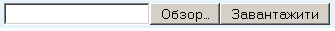
\includegraphics[scale=1,width=8cm]{ch05-01.png}
\caption{Форма завантаження файлу}
\label{f5-1:image}
\end{figure}

Перш, ніж приступити до написання сценарію обробки \verb'multipart'-форми, потрібно відредагувати файл конфігурації \verb'php.ini', щоб дозволити завантаження файлів на сервер.

Конфігураційний файл PHP php.ini має три параметри, пов'язані з завантаженням файлів на сервер:
\begin{enumerate}
\item \verb'file_uploads = On'~--- дозволяє завантаження файлів на сервер по протоколу HTTP;
\item \verb'upoad_tmp_dir = /tmp'~--- встановлює каталог для тимчасового зберігання завантажених файлів;
\item \verb'upload_max_filesize = 2M'~--- встановлює максимальний обсяг завантажуваних файлів. 

\end{enumerate}

Для успішного завантаження та збереження файлу необхідно створити сценарій виду:


\begin{lstlisting}[caption=Завантаження файлу на сервер]
<html>
<head>
  <title> Результат завантаження файлу </title>
</head>
<body>
<?php
if($_FILES["filename"]["size"] > 1024*3*1024)
   {
   echo ("Розмір файлу перевищує три мегабайта");
   exit;
   }
// Перевіряємо	чи	завантажився	файл
if(is_uploaded_file($_FILES["filename"]["tmp_name"]))
   {
   // Якщо так, то переносимо його у кінцевий каталог
   move_uploaded_file($_FILES["filename"]["tmp_name"], 
   "/path/to/file/".$_FILES["filename"]["name"]);
   } 
else 
   {
   echo("Помилка завантаження");
   }
?>
</body></html>
\end{lstlisting}

Слід зауважити, що для доступу до файлу використовується суперглобальний масив \verb'$_FILES', детальний опис якого дано у додатку~\ref{sup-glob:app}.



 
\pagebreak[3]
\section{Індивідуальне завдання}

\nopagebreak[4]
\subsection*{Завдання до лабораторної роботи}
\nopagebreak[4]
\begin{enumerate}
\item Вивчити теоретичний матеріал
\item Відповісти на контрольні запитання
\item Скласти алгоритм (блок-схему) програми
\item Виконати практичне завдання
\item Скласти звіт
\item Захистити роботу
\end{enumerate}

\subsection*{Контрольні запитання}
\nopagebreak[4]
\begin{enumerate}
\item Що таке файл? Що таке каталог?
\item Які основні операції для роботи з файлами ви знаєте?
\item Яким чином можна відкрити/створити файл у РНР?
\item Яким чином проводиться читання з файлу?
\item Яким чином проводиться запис у файл?
\item Яким чином можна переміщувати покажчик у файлі?
\item Що таке блокування файлу?
\item Які види блокування файлів ви знаєте?
\item Які особливості видів блокування файлів?
\item Яким чином завантажити файл на сервер?

\end{enumerate}

\subsection*{Практичні завдання}
\nopagebreak[4]


\begin{enumerate}
\item[]Створити форму з текстовим полем вводу для шляху каталогу та вивести таку інформацію: 
\item список об'єктів каталогу, підкаталоги виділити іншим кольором
\item вивести тільки файли, та реалізувати можливість їх видалення
\item знайти підкаталоги першого рівня та вивести їхній зміст
\item знайти порожні підкаталоги першого рівня, вивести їхні імена та видалити їх
\item створити 10 підкаталогів, та по 10 файлів у кожному, вивести отримане дерево
\item []Написати просту гостьову книгу, що зберігає інформацію у файлах, яка буде записувати та виводити:
\item перші 10 повідомлень користувачів та час відправлення
\item перші 10 повідомлень користувачів та поставлений ними рейтинг від 1 до 10
\item 10 повідомлень з найвищим рейтингом
\item список повідомлень з можливістю їх видалення
\item список повідомлень з можливістю їх редагування
\item[]Продемонструвати роботу гостьової книги 
\item[]Створити книгу рецептів, серед функцій якої є: 
\item виведення рецепту з найвищим рейтингом
\item виведення найсвіжіших рецептів
\item виведення найперших рецептів
\item збереження рецептів в окремих файлах
\item видалення вибраного рецепту
\item редагування вибраного рецепту
\item[]Продемонструвати роботу книги рецептів 
\item[]Створити фотогалерею з функціями додавання фотографії та опису до неї та додатковими функціями: 
\item виведення посилань на фото
\item виведення посилань на опис
\item виведення списку фото та видалення обраного
\item виведення списку та редагування опису обраного
\item обмежити розмір файлу, що завантажується до 1МБ
\item[]Продемонструвати роботу фотогалереї  
\item[]Створити файлове сховище з можливістю завантаження файлу та опису до нього та додатковими функціями:
\item вивести опис файлу та посилання для завантаження
\item реалізувати можливість видалення файлу
\item реалізувати можливість редагування імені файлу
\item реалізувати можливість редагування опису
\item[]Продемонструвати роботу файлового сховища 
\end{enumerate}


%\chapter{Сесії у РНР. Відправлення e-mail}
\section*{Мета роботи}
Навчитися використовувати сесії РНР та cookies. Розібратися в механізмі роботи сесій та cookies. Навчитися використовувати вбудовані засоби відправлення e-mail.
\section{Авторизація доступу}
У сучасних, навіть не дуже складних, веб-системах виникає потреба ідентифікувати користувача та виділити йому окреме поле діяльності. Якщо інформацію про ім'я, пароль та права користувача можна зберігати у файлах або у таблиці бази даних, то залишається проблема стеження за наявністю користувача на сайті.

Цю проблему можна вирішити двома способами:
\begin{itemize}
\item встановленням \verb'cookies'
\item запуском сесії.
\end{itemize}

Механізм сесій налаштований таким чином, що використовує механізм \verb'cookies' для передачі даних, але можливо обходитись і без \verb'cookies' у разі, коли вони відключені у користувача.
\section{Механізм сесії. Налаштування сесії}
\index{PHP!сесії}
\textbf{Сесія}~--- це механізм, який дозволяє створювати і використовувати змінні, зберігають своє значення протягом всього часу роботи користувача з сайтом.

Ці змінні для кожного користувача мають різні значення і можуть використовуватися на будь-якій сторінці сайту до виходу користувача з системи. При цьому кожного разу, заходячи на сайт, користувач отримує нові значення змінних, що дозволяють ідентифікувати його протягом цього сеансу або сесії роботи з сайтом. Звідси й назва механізму~--- сесії. 

Ідентифікатор сесії є 128 бітним числом. Якщо людина прийшла на сайт вперше і PHP-процесор це бачить, то даним відвідувачу присвоюється число, не присвоєне ще нікому. Надалі, при повторному заході, відвідувач буде асоційований з його особистим числом (ідентифікатором), через що програмі буде надана персональна область пам'яті.

Подання ідентифікатору сесії здійснюється у вигляді рядку із 32-х байт. Приклади ідентифікаторів сесії:

\begin{itemize}
\item \verb'7f4cbf53fbcd4717792447f32da7dba8'
\item \verb'ac4f4a45bdc893434c95dcaffb1c1811'
\end{itemize}

Налаштування PHP, в тому числі і для роботи з сесіями, прописуються у файлі \verb'php.ini'. В додатку~\ref{ses-opt:table} та~\ref{ses-opt-full:table} дано базові налаштування механізму сесії.

\subsection*{Унікальність сесій}
Підробити сесію або ідентифікатор не можна. Число з 128 біт (це 2 в 128 ступеня) в десятковому поданні має 38 нулів. Припустимо, на Вашому сайті буде 10~000 відвідувачів. Тоді у хакера шанси кілька зростають до 2 в ступені 114. Але це так само нереальна ймовірність~--- що-небудь підробити. Одна з очевидних причин наступна. Щоб підібрати номер сесії, потрібно зробити запит до Вашого веб-сервера. Нехай кожен запит займає 1024 байти. Через мільярд звернень до Вашого сайту, що складе 1000 ГБ трафіку, явно щось трапиться: Ваш сайт відключать через дикого трафіку або у вас не вистачить грошей на оплату такого великого трафіку. Ваш канал або пропускна здатність провайдера занадто слабка, щоб в розумні терміни перебрати всі номери. Ваш сервер не зможе хоч якось швидко працювати, маючи гігантську кількість пустих файлів, через створення фіктивних сесій. Ваш сервер переповниться лог-файлами і файлами фіктивних сесій, перестане працювати.

\subsection*{Збереження даних сесій}
Є два популярних способи зберігання даних сесій: база даних і файли. Ще можна зберігати сесії в пам'яті сервера (ОЗУ), але при виключенні сервера усі дані будуть втрачені. Зазвичай сесії зберігають у файлах, щоб знизити навантаження на базу даних. У деяких випадках сесії дозволяють повністю відмовитися від бази даних або використовувати її мінімально: в базі даних тільки список логінів/паролів, в сесіях (на файлах) вся робоча інформація.

За замовчуванням PHP зберігає всі в файлах (у своєму форматі) і сам дістає з них збережені дані. Після роботи кожного сценарію PHP сам все записує назад в особистий файл.

\subsection*{Передача ідентифікатора сесії}
Для передачі ідентифікатора сесії існують два основних способи і кілька маловживаних. Розглянемо скорочено механізм їх роботи:

\begin{enumerate}
\item \textbf{Cookies}

Це самий популярний і ефективний спосіб передачі ідентифікатора. Можна один раз помістити в куку змінну і всі інші скрипти будуть її отримувати. Якщо у користувача куки включені, PHP сам помістить туди ідентифікатор і потім сам його звідти дістане. 

Якщо у користувача куки вимкнені, то робота з сайтом може стати неможливою.

\item \textbf{параметри}
\begin{verse}
http://php.spb.ru/test.php?PHPSESSID=ac4f4a45bdc893434c95dcaffb1c1811
\end{verse}

Якщо ви будете дописувати всі ваші посилання подібним чином, то всі ваші наступні скрипти отримають ідентифікатор. PHP використовує і даний метод за замовчуванням (поєднуючи з куками, якщо ті вимкнені). Тобто PHP сам застосує або куки, або отриманий параметр.

Використання такого способу э 100\% надійним, але являється украй небезпечним, т.я. будь-хто може підробити параметр і отримати конфіденціальні дані користувача.

\item \textbf{PathInfo}
\begin{verse}
http://php.spb.ru/test.php/ac4f4a45bdc893434c95dcaffb1c1811
\end{verse}

Це засновано на розумінні веб-сервером того, де з цього URL шлях до скрипта, а де параметри. Тобто Апач розпізнає даний виклик, як звернення до файлу test.php і передасть йому рядок у змінній \verb'$pathinfo = getenv ("PATH_INFO")'. Відповідно, щоб передати управління в інший скрипт, треба подібним чином скласти URL (GET-запит) або передати форму GET або POST запитом.

\item Існують ще методи передачі ідентифікатора сесії, але вони ще менш зручні та не можуть надати надійного захисту від підробки.

\end{enumerate}



\section{Створення сесії, реєстрація змінних сесії, видалення змінних сесії}
\index{PHP!сесії!змінні сесії}
\index{PHP!функції!сесії}
При роботі із сесією виділяють три наступні етапи:
\begin{enumerate}
\item відкриття сесії
\item реєстрація змінних та їх використання
\item закриття сесії
\end{enumerate}
Нижче буде розглянуто всі три етапи.

\subsection*{Створення сесії}
Перше, що потрібно зробити для роботи з сесіями (якщо вони вже налаштовані адміністратором сервера), це запустити механізм сесій. Якщо в налаштуваннях сервера змінна \verb'session.auto_start = 0' (якщо \verb'session.auto_start = 1', то сесії запускаються автоматично), то будь-який скрипт, в якому потрібно використовувати дані сесії, повинен починатися з команди
\begin{verbatim}
  session_start(); 
\end{verbatim}

Отримавши таку команду, сервер створює нову сесію або відновлює поточну, ґрунтуючись на ідентифікаторі сесії, переданому за запитом.  Інтерпретатор PHP шукає змінну, в якій зберігається ідентифікатор сесії (за замовчуванням це \verb'PHPSESSID') спочатку в \verb'cookies', потім у змінних, переданих за допомогою \verb'POST' і \verb'GET'-запитів. Якщо ідентифікатор знайдений, то користувач вважається ідентифікованим, проводиться заміна всіх URL і виставляння \verb'cookies'. В іншому випадку користувач вважається новим, для нього генерується новий унікальний ідентифікатор, потім проводиться заміна URL і виставляння \verb'cookies'.

Нижче дано приклад роботи сесії:

\begin{verbatim}
<?
session_start(); 
echo session_id(); 
?>
<html>
<head><title>My home page</title></head>
... // домашняя страничка
</html>
<?
echo session_name(); 
?>
\end{verbatim}

Якщо оновити таку сторінку, то буде видно, що рядок, котрий друкує \verb'echo session_id();', не змінюється. Це вказує на те, що оновлення сесії проводиться успішно. Якщо закрити вікно браузера та відкрити цю сторінку знову, \verb'echo session_id();' видасть нове значення, томущо \verb'cookies' з минулої сесії вже знищено.


\subsection*{Реєстрація змінних}
Однак від самих ідентифікатора та імені сесії нам користі для вирішення завдань небагато. На практиці необхідно передавати щонайменше логін та пароль користувача. Для того щоб цього досягти, потрібно просто зареєструвати свої змінні:
\begin{verbatim}
session_register (ім'я_змінної1, 
        ім'я_змінної2, ...); 
\end{verbatim}
Зауважимо, що реєструються не значення, а імена змінних. Зареєструвати змінну досить один раз на будь-якій сторінці, де використовуються сесії. Імена змінних передаються функції \verb'session_register()' без знака <<\$>>. Всі зареєстровані таким чином змінні стають глобальними протягом даної сесії роботи з сайтом. 



\subsection*{Видалення змінних, сесії}
Крім вміння реєструвати змінні сесії (тобто робити їх глобальними протягом усього сеансу роботи), корисно також вміти видаляти такі змінні і сесію в цілому.

Функція \verb|session_unregister(ім'я_змінної)| видаляє глобальну змінну з поточної сесії (тобто видаляє її зі списку зареєстрованих змінних). Якщо реєстрація проводилася за допомогою \verb'$_SESSION', то використовують мовну конструкцію \verb'unset()'. Вона не повертає ніякого значення, а просто знищує зазначені змінні. Для того щоб скинути значення всіх змінних сесії, можна використовувати функцію \verb'session_unset();'.

Знищити поточну сесію цілком можна командою \verb'session_destroy();'. Вона не скидає значення глобальних змінних сесії і не видаляє \verb'cookies', а знищує всі дані, асоційовані з поточною сесією.

Перелік згаданих вище функцій дано у додатку~\ref{ses-func:text}. 
\section{Робота з cookies}
\index{PHP!cookies}

\textbf{Cookies}~--- це механізм зберігання даних браузером віддаленого комп'ютера для ідентифікації відвідувачів, що повертаються, та зберігання параметрів веб-сторінок (наприклад, змінних).

\textbf{Cookies}~--- це текстові рядки, що зберігаються на стороні клієнта, і містять пари <<ім'я-значення>>, з якими пов'язаний URL, по якому браузер визначає чи потрібно посилати \verb'cookies' на сервер.

Етапи роботи з  \verb'cookies' схожі на етапи використання механізму сесій:
\begin{enumerate}
\item встановлення \verb'cookies'
\item використання \verb'cookies'
\item видалення \verb'cookies'
\end{enumerate}
\subsection*{Встановлення cookies}
Встановлення cookies проводиться за допомогою функції \verb'setcookie()'. Ця функція має такі аргументи:
\begin{itemize}
\item \verb'name'~--- ім'я встановлюваного cookie;
\item \verb'value'~--- значення, яке зберігається в \verb'cookie' з ім'ям name;
\item \verb'expire'~--- час в секундах з початку епохи, по витікання якого поточний \verb'cookie' стає недійсним;
\item \verb'path'~--- шлях, по якому доступний cookie;
\item \verb'domain'~--- домен, з якого доступний cookie;
\item \verb'secure'~--- директива, яка визначає, чи доступний \verb'cookie' не по запиту HTPPS. За замовчуванням ця директива має значення 0, що означає можливість доступу до \verb'cookie' по звичайному запитом HTTP. 
\end{itemize}

При використанні Cookies необхідно мати на увазі, що Cookies повинні встановлюватися до першого виводу інформації в браузер (наприклад, оперетором echo або висновком якої функції). Тому бажано встановлювати Cookies на самому початку скрипта. Cookies встановлюються за допомогою певного заголовка сервера, а якщо скрипт виводить небудь, то це означає, що починається тіло документа. В результаті Cookies не будуть встановлені і може бути виведено попередження. Для перевірки успішності установки Cookies можна використовувати такий метод:

\begin{verbatim}
<?php
if (SetCookie("Test","Value")) 
echo "<h3>Cookies успішно встановлено!</h3>";
?>
\end{verbatim}

Функція \verb'SetCookie()' повертає TRUE у разі успішного встановлення Cookie. У разі, якщо Cookie встановити не вдається \verb'SetCookie()' поверне FALSE і можливо, попередження (залежить від налаштувань PHP). 


\subsection*{Використання cookies}

Доступ до \verb'cookie' здійснюється через суперглобальний масив \verb'$_COOKIE["name"]', де <<name>>~--- ім'я параметру, значення котрого необхідно отримати.

При читанні значень Cookies звертайте увагу на перевірку існування Cookies, наприклад, використовуючи оператор \verb'isset()'. Або шляхом придушення виведення помилок опереатором <<@>>.

Приклад встановлення Cookie і подальшого його читання:
\begin{verbatim}
<? php
setcookie( "test" , "Hello" , time()+3600 );
echo @$_COOKIE['test'];
?>
\end{verbatim}

У прикладі нижче показано як створити лічильник завантажень сторінки:
\begin{lstlisting}[caption=Лічильник завантажень сторінки]
<?php
// Проверяем, был ли уже установлен Cookie 'Mortal',
// Если да, то читаем его значение,
// И увеличиваем значение счетчика обращений к странице:
if (isset($_COOKIE['Mortal'])) $cnt=$_COOKIE['Mortal']+1;
else $cnt=0;
// Устанавливаем Cookie 'Mortal' зо значением счетчика,
// С временем "жизни" до 18/07/29,
// То есть на очень долгое время:
setcookie("Mortal",$cnt,0x6FFFFFFF);
// Выводит число посещений (загрузок) этой страницы:
echo "<p>Вы посещали эту страницу <b>".@$_COOKIE['Mortal']."</b> раз</p>";
?>
\end{lstlisting}

\subsection*{Встановлення масиву cookies}

Ми може встановити масив Cookies, використовуючи квадратні дужки в іменах Cookies \verb'[]', а потім прочитати масив Cookies і значення цього масиву:

\begin{lstlisting}[caption=Масив Cookies]
 <? php
// Устанавливаем массив Cookies:
setcookie("cookie[1]","Первый");
setcookie("cookie[2]","Второй");
setcookie("cookie[3]","Третий");
// После перезагрузки страницы мы отобразим
// Состав массива Cookies 'cookie':
if (isset($_COOKIE['cookie']))   
{
foreach ($_COOKIE ['cookie'] as $name => $value )   
   {
   echo "$name : $value <br>";
   }
}
?> 
\end{lstlisting}

\subsection*{Видалення cookies}

Іноді виникає необхідність видалення Cookies. Зробити це нескладно, необхідно лише знову встановити Cookie з ідентичним ім'ям і порожнім параметром. Наприклад:
\begin{verbatim}
<? php
SetCookie("Test" , "" );
?> 
\end{verbatim}


\section{Відправлення e-mail}
\index{PHP!функції!mail()}
\index{PHP!e-mail}
Найпростіший спосіб відправити лист за допомогою PHP~--- скористатися стандартною функцією \verb'mail()'. Вона має наступний синтаксис:
\begin{verbatim}
bool mail(to, subject, message [, additional\_headers 
[, additional\_parameters]])
\end{verbatim}

Обов'язкові параметри:
\begin{itemize}
\item E-mail одержувача
\item Заголовок листа
\item Текст листа 
\end{itemize}

Необов'язкові параметри:
\begin{itemize}
\item Додаткові заголовки листи
\item Додаткові параметри командного рядка 
\end{itemize}
Повертає значення:
\begin{itemize}
\item true, якщо лист було прийнято до доставки
\item false, в іншому випадку. 
\end{itemize}
Найпростіший приклад її використання виглядає так:
\begin{verbatim}
<?php
mail("joecool@example.com" , "My Subject" , "Line 1\nLine 2\nLine 3" );
?>
\end{verbatim}
Якщо у Вас на екрані з'явилася помилка <<Fatal error: Call to undefined function: mail()>>, це означає, що або PHP зібраний без підтримки функції mail, або вона заборонена налаштуваннями сервера. Така практика останнім часом широко поширена на безкоштовних хостингових серверах. Якщо Ви зіткнулися з такою проблемою, скористайтеся можливістю відправки листів за допомогою сокетів (sockets). 


\section{Альтернатива <<mail()>>}
\index{Системні додатки!sendmail}
На сьогоднішній день поширені наступні способи відправки листів з php-скриптів:
\begin{enumerate}
\item За допомогою виклику функції mail
\item Безпосередньо викликом sendmail
\item За допомогою сокетів
\item Використовуючи COM-об'єкт 
\end{enumerate}
\subsection*{sendmail}
\begin{lstlisting}[caption=Використання sendmail]
<?php
$sendmail = "/usr/sbin/sendmail -t -f $sender -C /etc/sendmail.orig.cf";
$fd = popen($sendmail, "w");
fputs($fd, "To: recipient@example.com\r\n");
fputs($fd, "From: \"Sender Name\" <$sender>\r\n");
fputs($fd, "Subject: Finally\r\n");
fputs($fd, "X-Mailer: Mailer Name\r\n\r\n");
fputs($fd, $body);
pclose($fd);
?> 
\end{lstlisting}
\subsection*{Active-X (COM)}
\begin{lstlisting}[caption=Використання Active-X]
<?php
@$CDONTS = new COM("CDONTS.NewMail");

@$CDONTS->From = "from_user@domain.com";
@$CDONTS->To = "to_user@domain.com";
@$CDONTS->CC = "cc_user@domain.com";
@$CDONTS->BCC = "bcc_user@domain.com";

@$CDONTS->BodyFormat = 0;
@$CDONTS->MailFormat = 0;

//@$CDONTS->AttachFile("c:\file.txt");

@$CDONTS->Subject = "Using CDONTS with PHP4 and IIS";
@$CDONTS->Body = "Blah blah blah blah, bleh...";

@$CDONTS->Send();
@$CDONTS->Close();
?> 
\end{lstlisting}

У разі роботи з сокетом відправлення дещо ускладнюється. Роботу з сокетами буде розглянуто в наступних лабораторних роботах.

\pagebreak[3]
\section{Індивідуальне завдання}

\nopagebreak[4]
\subsection*{Завдання до лабораторної роботи}
\nopagebreak[4]
\begin{enumerate}
\item Вивчити теоретичний матеріал
\item Відповісти на контрольні запитання
\item Скласти алгоритм (блок-схему) програми
\item Виконати практичне завдання
\item Скласти звіт
\item Захистити роботу
\end{enumerate}

\subsection*{Контрольні запитання}
\nopagebreak[4]
\begin{enumerate}
\item Що таке сесії? Для чого вони потрібні?
\item Яким чином забезпечується унікальність сесій?
\item Де зберігаються дані сесії?
\item Як створити сесію? 
\item Яким чином додати та видалити змінну сесії?
\item Що таке cookies?
\item Як використовувати cookies?
\item Як створити та використати масив cookies?
\item Яким чином можна відправити електронний лист?
\item Які альтернативи відправлень електронних листів ви знаєте?
\end{enumerate}

\subsection*{Практичні завдання}
\nopagebreak[4]


\begin{enumerate}
\item[]Написати HTML-сторінку з полями вводу логіну та паролю та додати наступний функціонал:
\item створити гостьову книгу, що зберігає запис користувача, виводить його записи, та дозволяє додавати нові без повторної авторизації
\item створити гостьову книгу що виводить перелік повідомлень та дозволяє видаляти їх певному користувачу без повторної авторизації
\item створити книгу рецептів, що дозволяє додавати, та дивитись додані рецепти тільки власнику записів послідовно без повторної авторизації
\item створити книгу рецептів, що дозволяє одному користувачу додавати рецепти, а іншому~--- видаляти
\item створити фотогалерею, що дозволяє додавати зображення та виводити їх перелік без повторної авторизації
\item створити фотогалерею, що дозволяє додавати зображення та видаляти їх певному користувачу без повторної авторизації
\item створити декілька зв'язаних сторінок, для різних користувачів виводити різну інформацію
\item створити примітивний форум на кілька користувачів (авторизація, додавання повідомлення, виведення повідомлень та імен користувачів)
\item створити сайт зі статтями, дати можливість просмотру неавторизованим користувачам та додавання авторизованим
\item створити сайт за статтями, дати можливість певним користувачам видаляти їх, заборонити просмотр неавторизованим користувачам
\item створити примітивний форум на кілька користувачів (авторизація, додавання повідомлення, виведення повідомлень та імен користувачів), що працює виключно на cookies
\item створити гостьову книгу, що зберігає запис користувача, виводить його записи, та дозволяє додавати нові без повторної авторизації, книга працює виключно на cookies
\item створити книгу рецептів, що дозволяє одному користувачу додавати рецепти, а іншому~--- видаляти, книга працює виключно на cookies
\item створити фотогалерею, що дозволяє додавати зображення та виводити їх перелік без повторної авторизації, фотогалерею працює виключно на cookies
\item створити примітивний онлайн-щоденник (додавання записів, виведення списку записів)
\item створити примітивний онлайн-щоденник (додавання записів, виведення списку записів), авторизацію користувача проводити за допомогою cookies
\item створити простий калькулятор (<<+>>, <<->>, <<*>>, <</>>) та виводити історію користувацьких обчислень 
\item створити простий калькулятор (<<+>>, <<->>, <<*>>, <</>>) та виводити історію користувацьких обчислень, авторизацію користувача проводити за допомогою cookies
\item створити гостьову книгу що виводить перелік повідомлень та дозволяє видаляти їх певному користувачу без повторної авторизації, авторизацію користувача проводити за допомогою cookies
\item створити простий калькулятор (<<+>>, <<->>, <<*>>, <</>>), записувати історію обчислень та виводити її адміністратору сайту
\item створити сторінку, що виводить адміністратору логін та пароль користувачів, та дозволяє їх змінювати 
\item створити сторінку, що виводить адміністратору логін та привілеї користувача, та дає право надавати права адміністратора
\item створити сторінку, яка дозволяє адміністратору видаляти користувачів з системи
\item створити сторінку, яка дозволяє додавати користувачів в систему
\item  створити фотогалерею, що дозволяє додавати зображення та видаляти їх певному користувачу без повторної авторизації, авторизацію користувача проводити за допомогою cookies
\item[]Результати роботи виводити у браузері.

\end{enumerate}



\chapter{Взаємодія РНР з СКБД MySQL}
\section*{Мета роботи}
Навчитися працювати з СУБД MySQL, записувати та отримувати табличні дані. Опрацювати взаємодію мови РНР з СУБД MySQL.

\section{Мова запитів SQL, та типи даних у СУБД MySQL}
\index{MySQL!SQL}
\subsection*{Основні команди}
Команди SQL можна поділити на дві категорії:
\begin{itemize}
\item команди означення даних
\item команди обробки даних
\end{itemize}

Перша категорія команд відповідає за створення або видалення баз даних, таблиць баз даних, редагування структури таблиць та типів даних полів таблиць.
До цієї категорії належать наступні команди:

\begin{itemize}
\item CREATE
\item DROP
\item ALTER
\item RENAME
\end{itemize}

Друга категорія команд відповідає за внесення даних до таблиць, оновлення та видалення даних.
До цієї категорії належать наступні команди:

\begin{itemize}
\item SELECT
\item INSERT
\item DELETE
\item UPDATE
\item HANDLER
\item TRUNCATE
\item REPLACE
\item LOAD DATA INFILE
\item DO
\end{itemize}

Нижче більш детально розглянуто синтаксис команд.

\subsection*{Команди означення даних}
\subsubsection*{CREATE}
\index{MySQL!SQL!CREATE}
Для створення бази даних необхідно використати наступну послідовність команд:

\begin{verbatim}
CREATE DATABASE [IF NOT EXISTS] db_name
\end{verbatim}

Оператор \verb'CREATE DATABASE' створює базу даних з вказаним іменем. Якщо база даних вже існує і не зазначений ключовий параметр \verb'IF NOT EXISTS', то виникає помилка виконання команди. 

Скорочений вид синтаксису команди створення таблиці виглядає наступним чином:

\begin{verbatim}
 CREATE [TEMPORARY] TABLE [IF NOT EXISTS] 
 tbl_name [(create_definition, ...)]
 [Table_options] [select_statement]
\end{verbatim}

Оператор створює таблицю. Якщо таблиця вже існує і не зазначений параметр \verb'IF NOT EXISTS', то виникає помилка виконання команди. Параметри таблиці та перелік полів вказують після означення імені таблиці. Приклад створення таблиці надано нижче:
\begin{verbatim}
 CREATE TABLE table123 (f1 INT, f2 INT)
\end{verbatim}
Створюється таблиця з двома полями цілочисельного типу.

Повний перелік можливих параметрів команди дано у додатку~\ref{crtab:text}.

Для створення індексів у СУБД MySQL існує команда CREATE INDEX. Синтаксис команди надано нижче: 
\begin{verbatim}
 CREATE [UNIQUE | FULLTEXT] INDEX index_name
         ON tbl_name (col_name [(length)], ...)
\end{verbatim}
Команда CREATE INDEX у версіях MySQL до 3.22 не виконує ніяких дій. У версії 3.22 і більш пізніх CREATE INDEX відповідає команді ALTER TABLE в частині створення індексів. Зазвичай всі індекси створюються в таблиці під час створення самої таблиці командою CREATE TABLE. CREATE INDEX дає можливість додати індекси до існуючих таблиць.


\subsubsection*{DROP}
\index{MySQL!SQL!DROP}
Для видалення бази даних існує наступна команда:
\begin{verbatim}
 DROP DATABASE [IF EXISTS] db_name
\end{verbatim}
Оператор DROP DATABASE видаляє всі таблиці в зазначеній базі даних і саму базу. Якщо ви виконуєте DROP DATABASE на базі даних, символічно пов'язаної з іншою, то видаляється як посилання, так і оригінальна база даних. Будьте дуже уважні при роботі з цією командою!

Оператор DROP DATABASE повертає кількість файлів, які були видалені з директорії бази даних. Як правило, це число дорівнює кількості таблиць, помноженому на три, оскільки зазвичай кожна таблиця представлена трьома файлами: .MYD-файлом, MYI-файлом і .Frm-файлом.

Команда DROP DATABASE видаляє з директорії зазначеної бази даних всі файли з наступними розширеннями: <<.BAK>>, <<.DAT>>, <<.HSH>>, <<.ISD>>, <<.ISM>>, <<.ISM>>, <<.MRG>>, <<.MYD>>, <<.MYI>>, <<.Db>>, <<.Frm>>. 	

Всі піддиректорії, імена яких складаються з двох цифр (RAID-директорії), також видаляються.

У версії MySQL 3.22 і більш пізніх можна використовувати ключові слова IF EXISTS для попередження помилки, якщо зазначена база даних не існує. 

Щоб видалити таблицю з поточної бази даних необхідно виконати наступну команду: 
\begin{verbatim}
 DROP TABLE [IF EXISTS] tbl_name 
 [, tbl_name, ...] [RESTRICT | CASCADE]
\end{verbatim}
Оператор DROP TABLE видаляє одну або декілька таблиць. Всі табличні дані та визначення видаляються, так що будьте уважні при роботі з цією командою!

У версії MySQL 3.22 і більш пізніх можна використовувати ключові слова IF EXISTS , щоб попередити помилку, якщо зазначені таблиці не існують. 

Для видалення індексів з таблиць необхідно використати команду
\begin{verbatim}
 DROP INDEX index_name ON tbl_name
\end{verbatim}
Оператор DROP INDEX видаляє індекси, зазначені в index\_name з таблиці tbl\_name. DROP INDEX не виконує ніяких дій у версіях MySQL до 3.22. У версіях 3.22 і більш пізніх DROP INDEX відповідає команді ALTER TABLE в частині видалення індексів.
\subsubsection*{ALTER}
\index{MySQL!SQL!ALTER}
Скорочений синтаксис команди для зміни структури таблиць виглядає наступним чином:
\begin{verbatim}
 ALTER [IGNORE] TABLE tbl_name alter_spec 
 [, alter_spec ...]
\end{verbatim}
Оператор ALTER TABLE забезпечує можливість змінювати структуру існуючої таблиці. Наприклад, можна додавати або видаляти стовпці, створювати або знищувати індекси або перейменовувати стовпці або саму таблицю. Можна також змінювати коментар для таблиці та її тип.

Нижче надано приклади використання команди:

Для того щоб змінити тип стовпця з INTEGER на TINYINT NOT NULL (залишаючи ім'я колишнім) і змінити тип стовпця b з CHAR(10) на CHAR(20) з перейменуванням його з b на c :
\begin{verbatim}
ALTER TABLE t2 MODIFY a TINYINT NOT NULL, 
      CHANGE bc CHAR (20);
\end{verbatim}

Для того щоб додати індекс до стовпцю d і зробити стовпець a первинним ключем:
\begin{verbatim}
ALTER TABLE t2 ADD INDEX (d), ADD PRIMARY KEY (a);
\end{verbatim}

Повні дані щодо синтаксису ALTER TABLE дано в додатку~\ref{alttab:text}.

\subsubsection*{RENAME}
\index{MySQL!SQL!RENAME}
Для перейменування таблиць, починаючи з версії 3.22, введено команду RENAME TABLE.
\begin{verbatim}
 RENAME TABLE tbl_name TO new_tbl_name 
 [, tbl_name2 TO new_tbl_name2, ...]
\end{verbatim}
Операція перейменування повинна здійснюватися як атомарна, тобто при виконанні перейменування ніякому іншому потоку не дозволяється доступ до зазначених таблиць. Завдяки цьому можливе заміщення таблиці порожній таблицею:
\begin{verbatim}
 CREATE TABLE new_table (...);
 RENAME TABLE old_table TO backup_table, 
 new_table TO old_table;
\end{verbatim}
Перейменування проводиться зліва направо. Таким чином, для обміну іменами між двома таблицями необхідно виконати наступні дії:
\begin{verbatim}
 RENAME TABLE old_table TO backup_table,
         new_table TO old_table,
         backup_table TO new_table;
\end{verbatim}
Для двох баз даних, що знаходяться на одному і тому ж диску, можна також здійснювати обмін іменами:
\begin{verbatim}
 RENAME TABLE current_db.tbl_name 
 TO other_db.tbl_name;
\end{verbatim}
При виконанні команди RENAME не повинні мати місце заблоковані таблиці або активні транзакції. Необхідно також мати привілеї ALTER і DROP для початкової таблиці і привілеї CREATE і INSERT~--- для нової.

Якщо MySQL стикається з якою-небудь помилкою при перейменуванні декількох таблиць, то станеться зворотне перейменування для всіх перейменованих таблиць, щоб повернути все в початковий стан. 

\subsection*{Команди обробки даних}
\subsubsection*{SELECT}
\index{MySQL!SQL!SELECT}

Оператор SELECT має наступну структуру:
\begin{verbatim}
 SELECT [STRAIGHT_JOIN]
        [SQL_SMALL_RESULT] [SQL_BIG_RESULT] 
        [SQL_BUFFER_RESULT] [SQL_CACHE | SQL_NO_CACHE] 
        [SQL_CALC_FOUND_ROWS] [HIGH_PRIORITY]
        [DISTINCT | DISTINCTROW | ALL]
     select_expression, ...
     [INTO {OUTFILE | DUMPFILE} 
     'file_name' export_options]
     [FROM table_references
       [WHERE where_definition]
       [GROUP BY {unsigned_integer | 
       col_name | formula} [ASC | DESC], ...]
       [HAVING where_definition]
       [ORDER BY {unsigned_integer | 
       col_name | formula} [ASC | DESC], ...]
       [LIMIT [offset,] rows]
       [PROCEDURE procedure_name]
       [FOR UPDATE | LOCK IN SHARE MODE]]
\end{verbatim}
SELECT застосовується для вилучення рядків, вибраних з однієї або декількох таблиць. Вираз select\_expression задає стовпці, в яких необхідно проводити вибірку. Крім того, оператор SELECT можна використовувати для витягання рядків, обчислених без посилання якусь таблицю. Наприклад запит \verb'SELECT 1 + 1;' поверне значення <<2>>.

\subsubsection*{INSERT}
\index{MySQL!SQL!INSERT}
\begin{verbatim}
     INSERT [LOW_PRIORITY | DELAYED] 
         [IGNORE] [INTO] tbl_name [(col_name, ...)]
         VALUES (expression, ...), (...), ...
 або INSERT [LOW_PRIORITY | DELAYED] [IGNORE]
         [INTO] tbl_name [(col_name, ...)]
         SELECT ...
 або INSERT [LOW_PRIORITY | DELAYED] [IGNORE]
         [INTO] tbl_name
         SET col_name = expression, 
         col_name = expression, ...
\end{verbatim}
Оператор INSERT вставляє нові рядки в існуючу таблицю. Форма даної команди INSERT \dots VALUES вставляє рядки відповідно до точно зазначеними в команді значеннями. Форма INSERT \dots SELECT вставляє рядки, обрані з іншої таблиці або таблиць. Форма INSERT ... VALUES зі списком з декількох значень підтримується у версії MySQL 3.22.5 і більш пізніх. Синтаксис вираження col\_name=expression підтримується у версії MySQL 3.22.10 і більш пізніх. 

Команда INSERT \dots SELECT забезпечує можливість швидкого внесення великої кількості рядків у таблицю з однієї або більше таблиць.
\begin{verbatim}
 INSERT INTO tblTemp2 (fldID) 
         SELECT tblTemp1.fldOrder_ID 
         FROM tblTemp1
         WHERE tblTemp1.fldOrder_ID > 100;
\end{verbatim}

\subsubsection*{DELETE}
\index{MySQL!SQL!DELETE}
\begin{verbatim}
DELETE [LOW_PRIORITY | QUICK] FROM table_name
       [WHERE where_definition]
       [ORDER BY ...]
       [LIMIT rows]

или

DELETE [LOW_PRIORITY | QUICK] table_name[.*] [,table_name[.*] ...]
       FROM table-references
       [WHERE where_definition]

oили

DELETE [LOW_PRIORITY | QUICK]
       FROM table_name[.*], [table_name[.*] ...]
       USING table-references
       [WHERE where_definition]
\end{verbatim}
Оператор DELETE видаляє з таблиці table\_name рядки, що задовольняють заданим в where\_definition умовам, і повертає число віддалених записів.

Якщо оператор DELETE запускається без визначення WHERE, то видаляються всі рядки. При роботі в режимі AUTOCOMMIT це буде аналогічно використанню оператора TRUNCATE. В MySQL 3.23 оператор DELETE без визначення WHERE поверне нуль як число віддалених записів.
\subsubsection*{UPDATE}
\index{MySQL!SQL!UPDATE}

\begin{verbatim}
UPDATE [LOW_PRIORITY] [IGNORE] tbl_name
    SET col_name1=expr1 [, col_name2=expr2, ...]
    [WHERE where_definition]
    [LIMIT #]
\end{verbatim}
Оператор UPDATE оновлює стовпці відповідно до їх новими значеннями в рядках існуючої таблиці. У виразі SET вказується, які саме стовпці слід модифікувати і які величини повинні бути в них встановлені. У виразі WHERE, якщо воно присутнє, задається, які рядки підлягають оновленню. В інших випадках оновлюються всі рядки. Якщо задано вираз ORDER BY, то рядки будуть оновлюватися у зазначеному в ньому порядку.

Якщо вказується ключове слово LOW\_PRIORITY, то виконання даної команди UPDATE затримується до тих пір, поки інші клієнти не завершать читання цієї таблиці.

Якщо вказується ключове слово IGNORE, то команда оновлення не буде перервана, навіть якщо при оновленні виникне помилка дублювання ключів. Рядки, через які виникають конфліктні ситуації, оновлені не будуть.

Якщо доступ до стовпцю із зазначеного виразу здійснюється по аргументу tbl\_name, то команда UPDATE використовує для цього стовпця його поточне значення.
\subsubsection*{HANDLER}
\index{MySQL!SQL!HANDLER}
Оператор HANDLER забезпечує прямий доступ до інтерфейсу дескриптора таблиці MyISAM, минаючи оптимізатор SQL. Отже, цей оператор працює швидше, ніж SELECT.

Перша форма оператора HANDLER відкриває таблицю, роблячи її доступною для послідовності команд HANDLER \dots READ. Цей об'єкт недоступний іншим потокам і не буде закритий, поки даний потік не викличе HANDLER tbl\_name CLOSE або сам потік не буде знищений.

Друга форма вибирає один рядок (або більше - у відповідності з установкою в вираженні LIMIT), для якої (их) зазначений індекс відповідає заданій умові і умова в виразі WHERE також виконується. Якщо індекс складається з декількох частин (охоплює декілька стовпців), то складові його величини вказуються у вигляді розділеного комами списку. Забезпечуються величини тільки для декількох перших шпальт.

Третя форма вибирає один рядок (або більше - у відповідності з установкою в вираженні LIMIT), з таблиці; гаразд вказівки індексів у відповідності з умовою WHERE.

Четверта форма (без зазначення індексів) вибирає один рядок (або більше - у відповідності з установкою в вираженні LIMIT), з таблиці, використовуючи природний порядок рядків (як вони зберігаються у файлі даних), у відповідності з умовою WHERE. Ця форма працює швидше, ніж HANDLER tbl\_name READ index\_name, в тих випадках, коли бажаний перегляд всієї таблиці.

Оператор HANDLER \dots CLOSE закриває таблицю, відкриту оператором HANDLER ... OPEN.
\subsubsection*{TRUNCATE}
\index{MySQL!SQL!TRUNCATE}
\begin{verbatim}
TRUNCATE TABLE table_name
\end{verbatim}
TRUNCATE TABLE має наступні відмінності від DELETE FROM ...:
\begin{itemize}
\item Ця операція видаляє і відтворює таблицю, що набагато швидше, ніж почергове видалення рядків.
\item Операція є нетранзакціонной; якщо одночасно виконується транзакція або активна блокування таблиці, то можна отримати помилку.
\item Не повертає кількість вилучених рядків.
\item Поки існує коректний файл <<table\_name.frm>>, таблицю можна відтворити з його допомогою, навіть якщо файли даних або індексів пошкоджені.
\end{itemize}

TRUNCATE є розширенням Oracle SQL.
\subsubsection*{REPLACE}
\index{MySQL!SQL!REPLACE}
\begin{verbatim}
    REPLACE [LOW_PRIORITY | DELAYED]
        [INTO] tbl_name [(col_name,...)]
        VALUES (expression,...),(...),...
или REPLACE [LOW_PRIORITY | DELAYED]
        [INTO] tbl_name [(col_name,...)]
        SELECT ...
или REPLACE [LOW_PRIORITY | DELAYED]
        [INTO] tbl_name
        SET col_name=expression, col_name=expression,...
\end{verbatim}

Оператор REPLACE працює точно так само, як INSERT, за винятком того, що якщо стара запис у даній таблиці має те ж значення індексу UNIQUE або PRIMARY KEY, що і нова, то стара запис перед занесенням нової буде видалена.

\subsubsection*{LOAD DATA INFILE}
\index{MySQL!SQL!LOAD DATA INFILE}

\begin{verbatim}
LOAD DATA [LOW_PRIORITY | CONCURRENT] [LOCAL] INFILE 'file_name.txt'
    [REPLACE | IGNORE]
    INTO TABLE tbl_name
    [FIELDS
        [TERMINATED BY '\t']
        [[OPTIONALLY] ENCLOSED BY '']
        [ESCAPED BY '\\' ]
    ]
    [LINES TERMINATED BY '\n']
    [IGNORE number LINES]
    [(col_name,...)]
\end{verbatim}

Команда LOAD DATA INFILE читає рядки з текстового файлу і вставляє їх у таблицю з дуже високою швидкістю. Якщо задано ключове слово LOCAL, то файл читається з клієнтського хоста. Якщо ж LOCAL не вказується, то файл повинен знаходитися на сервері. (Опція LOCAL доступна у версії MySQL 3.22.6 і більш пізніх.)

Якщо текстові файли, які потрібно прочитати, знаходяться на сервері, то з міркувань безпеки ці файли повинні або розміщуватися в директорії бази даних, або бути доступними для читання всім користувачам. Крім того, для застосування команди LOAD DATA INFILE до серверних файлів необхідно володіти привілеями FILE для серверного хосту.


\subsubsection*{DO}
\index{MySQL!SQL!DO}

\begin{verbatim}
DO expression, [expression, ...]
\end{verbatim}
Виконує даний вираз, але не повертає небудь результат. Є скороченою формою оператора SELECT expression, expression, але перевага його полягає в тому, що він працює трохи швидше, якщо немає необхідності в поверненні результату.

Оператор головним чином корисний при використанні з функціями, які мають побічні ефекти, такими як RELEASE\_LOCK.
\section{Функції для роботи з MySQL. Виконання SQL-запитів}
\index{MySQL!PHP!функції}

\section{Установка з'єднання. Вибір бази даних}
\index{MySQL!таблиці}

\section{Вибірка з таблиці, розбір результату вибірки}
\index{MySQL!вибірка}

\section{Додавання записів, оновлення записів}
\index{MySQL!додавання}
\index{MySQL!оновлення}
\section{Очищення і видалення таблиць}
\index{MySQL!очищення таблиць}
\index{MySQL!видалення таблиць}
\pagebreak[3]
\section{Індивідуальне завдання}

\nopagebreak[4]
\subsection*{Завдання до лабораторної роботи}
\nopagebreak[4]
\begin{enumerate}
\item Вивчити теоретичний матеріал
\item Відповісти на контрольні запитання
\item Скласти алгоритм (блок-схему) програми
\item Виконати практичне завдання
\item Скласти звіт
\item Захистити роботу
\end{enumerate}

\subsection*{Контрольні запитання}
\nopagebreak[4]
\begin{enumerate}
\item Що таке рядки?
\item Яким чином можна задати рядковий літерал?
\item Яка особливість рядків у подвійних лапках?
\item Яка особливість синтаксису \verb'Heredoc'? 
\item Яким чином вивести HTML-код на веб-сторінці?
\item Що таке регулярні вирази?
\item Яка особливість метасимволу <<\verb'\'>>?
\item Для чого використвуються регулярні вирази?
\item Які функції для роботи з регулярними виразами ви знаєте?
\item Яким чином можна використовувати регулярні вирази в SQL-запитах?
\end{enumerate}

\subsection*{Практичні завдання}
\nopagebreak[4]


\begin{enumerate}
\item[]Написати HTML-сторінку з формою, що складається з:
\item однорядкового поля вводу, поля вводу пароля та кнопки відправлення форми.
\item 

\end{enumerate}


\chapter{ООП. Робота з XML}
\index{PHP!ООП}
Хоча РНР володіє загальними об'єктно-орієнтованими можливостями, він не є повноцінною ОО-мовою (наприклад, такою, як C++ або Java). Зокрема, в РНР не підтримуються наступні об'єктно-орієнтовані можливості:
\begin{itemize}
\item множинне спадкування;
\item автоматичний виклик конструкторів (якщо ви хочете, щоб при конструюванні об'єкта похідного класу викликався конструктор базового класу, вам доведеться викликати його явно);
\item абстрактні класи;
\item перевантаження методів;
\item перевантаження операторів (це пов'язано з тим, що РНР є мовою з вільною типізацією);
закритий і відкритий доступ, віртуальні функції;
\item деструктори.
\end{itemize}

Але і без усього перерахованого ви все одно зможете отримати користь з об'єктно-орієнтованих можливостей, підтримуваних РНР. Реалізація ООП в РНР надає колосальну допомогу в модульному оформленні функціональності вашої програми.
\section{Класи та об'єкти. Методи}
\index{PHP!ООП!класи}
\index{PHP!ООП!об'єкти}
Класи утворюють синтаксичну базу об'єктно-орієнтованого програмування. Їх можна розглядати як свого роду <<контейнери>> для логічно пов'язаних даних і функцій (методів). Клас являє собою шаблон, по якому створюються конкретні екземпляри, використовуються в програмі. Екземпляри класів називаються об'єктами.

\subsection{Оголошення класу}
Клас можна розглядати як тип даних, а об'єкт~--- як змінну. Програма може одночасно працювати з декількома об'єктами одного класу як і з декількома змінними. Загальний формат класів РНР приведений в наступному лістингу.

\begin{lstlisting}[caption=Синтаксис оголошення класів]
class Class_name {
var $attribute_1;
//...
var $attribute_N;
function function1() {
//...
}
//...
function functionN() {
//...
}
} // end Class_name 
\end{lstlisting}

Оголошення класу має починатися з ключового слова \verb|class| (подібно до того, як оголошення функції починається з ключового слова \verb|function|). Кожному оголошенню атрибуту, що міститься в класі, має передувати ключове слово \verb|var|. Атрибути можуть відноситися до будь-якого типу даних, підтримуваних в РНР. Після оголошень атрибутів слідують оголошення методів, дуже схожі на типові оголошення функцій.

Методи часто використовуються для роботи з атрибутами класів. При посиланнях на атрибути всередині методів використовується спеціальна змінна \verb|$this|. Синтаксис методів продемонстрований в наступному прикладі:

\begin{lstlisting}[caption=Приклад створення методів]
<?
class Webpage {
var $bgcolor;
function setBgColor($color) {
$this->bgcolor = $color;
}
function getBgColor() {
return $this->bgcolor;
}
}
?> 
\end{lstlisting}

Змінна \verb|$this| посилається на екземпляр об'єкта, для якого викликається метод. Оскільки в будь-якому класі може існувати декілька екземплярів об'єктів, уточнення \verb|$this| необхідно для посилань на атрибути, що належать поточному об'єкту. При використанні цього синтаксису зверніть увагу на дві обставини:

\begin{enumerate}
\item атрибут, на який ви посилаєтеся в методі, не потрібно передавати у вигляді параметра функції;
\item знак долара (\$) ставиться перед змінною \verb|$this|, але не перед ім'ям атрибута (як у звичайної змінної).
\end{enumerate}

\subsection{Створення об'єкта}


\section{Наслідування}
\index{PHP!ООП!наслідування}

\section{Конструктори та деструктори}
\index{PHP!ООП!коснструктори}
\index{PHP!ООП!Деструктори}

Досить часто при створенні об'єкта потрібно задати значення деяких атрибутів. На щастя, розробники технології ООП врахували цю обставину і реалізували його в концепції конструкторів. Конструктор являє собою метод, який задає значення деяких атрибутів (а також може викликати інші методи). Конструктори викликаються автоматично при створенні нових об'єктів. Щоб це стало можливим, ім'я методу-конструктора повинне збігатися з ім'ям класу, в якому він міститься. Приклад конструктора приведений в лістингу 2.

\section{Оператори <<::>> та <<parent>>}
\index{PHP!ООП!<<::>>}
\index{PHP!ООП!<<parent>>}


\section{Об'єктна модель XML-документа}
\index{PHP!XML}
\section{Розширення SAX та DOM для роботы з XML}
\index{PHP!XML!SAX}
\index{PHP!XML!DOM}

\pagebreak[3]
\section{Індивідуальне завдання}

\nopagebreak[4]
\subsection*{Завдання до лабораторної роботи}
\nopagebreak[4]
\begin{enumerate}
\item Вивчити теоретичний матеріал
\item Відповісти на контрольні запитання
\item Скласти алгоритм (блок-схему) програми
\item Виконати практичне завдання
\item Скласти звіт
\item Захистити роботу
\end{enumerate}

\subsection*{Контрольні запитання}
\nopagebreak[4]
\begin{enumerate}
\item Що таке рядки?
\item Яким чином можна задати рядковий літерал?
\item Яка особливість рядків у подвійних лапках?
\item Яка особливість синтаксису \verb'Heredoc'? 
\item Яким чином вивести HTML-код на веб-сторінці?
\item Що таке регулярні вирази?
\item Яка особливість метасимволу <<\verb'\'>>?
\item Для чого використвуються регулярні вирази?
\item Які функції для роботи з регулярними виразами ви знаєте?
\item Яким чином можна використовувати регулярні вирази в SQL-запитах?
\end{enumerate}

\subsection*{Практичні завдання}
\nopagebreak[4]


\begin{enumerate}
\item[]Написати HTML-сторінку з формою, що складається з:
\item однорядкового поля вводу, поля вводу пароля та кнопки відправлення форми.
\item 

\end{enumerate}


\chapter{Робота з сокетами. Пересилання даних JSON}
\section{Структура сокета. Відкриття та закриття сокета}
\index{PHP!сокет}

\section{Запис в сокет та читання з сокета}
\section{Синтаксис JSON, його структура}
\index{JSON}

\section{Кодування та декодування JSON у РНР}
\index{JSON!PHP}
\index{PHP!JSON}
\section{Обмін даними з JavaScript-додатками}
\index{JSON!JavaScript}


\pagebreak[3]
\section{Індивідуальне завдання}

\nopagebreak[4]
\subsection*{Завдання до лабораторної роботи}
\nopagebreak[4]
\begin{enumerate}
\item Вивчити теоретичний матеріал
\item Відповісти на контрольні запитання
\item Скласти алгоритм (блок-схему) програми
\item Виконати практичне завдання
\item Скласти звіт
\item Захистити роботу
\end{enumerate}

\subsection*{Контрольні запитання}
\nopagebreak[4]
\begin{enumerate}
\item Що таке рядки?
\item Яким чином можна задати рядковий літерал?
\item Яка особливість рядків у подвійних лапках?
\item Яка особливість синтаксису \verb'Heredoc'? 
\item Яким чином вивести HTML-код на веб-сторінці?
\item Що таке регулярні вирази?
\item Яка особливість метасимволу <<\verb'\'>>?
\item Для чого використвуються регулярні вирази?
\item Які функції для роботи з регулярними виразами ви знаєте?
\item Яким чином можна використовувати регулярні вирази в SQL-запитах?
\end{enumerate}

\subsection*{Практичні завдання}
\nopagebreak[4]


\begin{enumerate}
\item[]Написати HTML-сторінку з формою, що складається з:
\item однорядкового поля вводу, поля вводу пароля та кнопки відправлення форми.
\item 

\end{enumerate}

\chapter{Робота з зображеннями}
\index{PHP!зображення}
\index{PHP!GD}
\section{Створення зображень}
\section{Малювання простих геометричних фігур}
\section{Малювання тексту на зображенні}
\section{Зміна розміру зображення}
\section{Функції бібліотеки GD}


\pagebreak[3]
\section{Індивідуальне завдання}

\nopagebreak[4]
\subsection*{Завдання до лабораторної роботи}
\nopagebreak[4]
\begin{enumerate}
\item Вивчити теоретичний матеріал
\item Відповісти на контрольні запитання
\item Скласти алгоритм (блок-схему) програми
\item Виконати практичне завдання
\item Скласти звіт
\item Захистити роботу
\end{enumerate}

\subsection*{Контрольні запитання}
\nopagebreak[4]
\begin{enumerate}
\item Що таке рядки?
\item Яким чином можна задати рядковий літерал?
\item Яка особливість рядків у подвійних лапках?
\item Яка особливість синтаксису \verb'Heredoc'? 
\item Яким чином вивести HTML-код на веб-сторінці?
\item Що таке регулярні вирази?
\item Яка особливість метасимволу <<\verb'\'>>?
\item Для чого використвуються регулярні вирази?
\item Які функції для роботи з регулярними виразами ви знаєте?
\item Яким чином можна використовувати регулярні вирази в SQL-запитах?
\end{enumerate}

\subsection*{Практичні завдання}
\nopagebreak[4]


\begin{enumerate}
\item[]Написати HTML-сторінку з формою, що складається з:
\item однорядкового поля вводу, поля вводу пароля та кнопки відправлення форми.
\item 

\end{enumerate}

\appendix
\makeatletter
\gdef\thechapter{\@Asbuk\c@chapter}
\makeatother
\def\chaptername{Додаток}


\chapter{Правила оформлення звіту}
\section{Титульна сторінка лабораторної роботи}
%\begin{titlepage}
%\newpage

\hrulefill

\begin{center}
МІНІСТЕРСТВО ОСВІТИ І НАУКИ, МОЛОДІ ТА СПОРТУ УКРАЇНИ \\

ХЕРСОНСЬКИЙ НАЦІОНАЛЬНИЙ ТЕХНІЧНИЙ УНІВЕРСИТЕТ \\*

КАФЕДРА ІНФОРМАЦІЙНИХ ТЕХНОЛОГІЙ

\end{center}

\vspace{5em}

\begin{center}
\Large Звіт до лабораторної роботи \No 123 \\ з дисципліни <<Web-програмування>>
\end{center}

\vspace{2.5em}

\begin{center}
{\Large Тема: \textbf{<<Основи мережі Internet>>}}
\end{center}

\vspace{5em}





\begin{flushleft}
Виконав \\ст.групи хПР1 \hspace{\fill} Пупкін А.А. \\
\vspace{1em}
Перевірив \\ст.викладач \hspace{\fill} Іванов Б.Б.\\
\end{flushleft}

\vspace{\fill}

\begin{center}
Херсон 2012
\end{center}
\newpage
%\end{titlepage}
\section{Приклади блок-схем}
Правила виконання блок-схем задані наступними документами:
\begin{itemize}
\item ГОСТ 19.701-90. Схемы алгоритмов, программ, данных и систем. Условные обозначения и правила выполнения
\item ГОСТ 19.002-80. Схемы алгоритмов и программ. Правила выполнения
\item ГОСТ 19.003-80. Схемы алгоритмов и программ. Обозначения условные графические

\end{itemize}




\begin{longtable}[t]{|c|p{6em}|p{15em}|}

\caption{\space Основны елементи блок-схем} \label{bl-ch:table}\\
\hline

Найменування & Позначення & Призначення \\
\hline \endfirsthead
\caption*{\space Продовження} \\
\hline
Найменування & Позначення & Призначення \\
\hline \endhead
\hline \endfoot



Блок початок-кінець &  % Graphic for TeX using PGF
% Title: C:\Documents and Settings\Admin\Мои документы\Мои рисунки\Диаграмма1.dia
% Creator: Dia v0.97.2
% CreationDate: Sat Sep 08 10:27:27 2012
% For: Admin
% \usepackage{tikz}
% The following commands are not supported in PSTricks at present
% We define them conditionally, so when they are implemented,
% this pgf file will use them.
\ifx\du\undefined
  \newlength{\du}
\fi
\setlength{\du}{15\unitlength}
\begin{tikzpicture}
\pgftransformxscale{1.000000}
\pgftransformyscale{-1.000000}
\definecolor{dialinecolor}{rgb}{0.000000, 0.000000, 0.000000}
\pgfsetstrokecolor{dialinecolor}
\definecolor{dialinecolor}{rgb}{1.000000, 1.000000, 1.000000}
\pgfsetfillcolor{dialinecolor}
\pgfsetlinewidth{0.100000\du}
\pgfsetdash{}{0pt}
\pgfsetdash{}{0pt}
\pgfsetbuttcap
\pgfsetmiterjoin
\pgfsetlinewidth{0.100000\du}
\pgfsetbuttcap
\pgfsetmiterjoin
\pgfsetdash{}{0pt}
\definecolor{dialinecolor}{rgb}{1.000000, 1.000000, 1.000000}
\pgfsetfillcolor{dialinecolor}
\pgfpathmoveto{\pgfpoint{5.632500\du}{0.350000\du}}
\pgfpathlineto{\pgfpoint{8.362500\du}{0.350000\du}}
\pgfpathcurveto{\pgfpoint{8.739435\du}{0.350000\du}}{\pgfpoint{9.045000\du}{0.641015\du}}{\pgfpoint{9.045000\du}{1.000000\du}}
\pgfpathcurveto{\pgfpoint{9.045000\du}{1.358985\du}}{\pgfpoint{8.739435\du}{1.650000\du}}{\pgfpoint{8.362500\du}{1.650000\du}}
\pgfpathlineto{\pgfpoint{5.632500\du}{1.650000\du}}
\pgfpathcurveto{\pgfpoint{5.255565\du}{1.650000\du}}{\pgfpoint{4.950000\du}{1.358985\du}}{\pgfpoint{4.950000\du}{1.000000\du}}
\pgfpathcurveto{\pgfpoint{4.950000\du}{0.641015\du}}{\pgfpoint{5.255565\du}{0.350000\du}}{\pgfpoint{5.632500\du}{0.350000\du}}
\pgfusepath{fill}
\definecolor{dialinecolor}{rgb}{0.000000, 0.000000, 0.000000}
\pgfsetstrokecolor{dialinecolor}
\pgfpathmoveto{\pgfpoint{5.632500\du}{0.350000\du}}
\pgfpathlineto{\pgfpoint{8.362500\du}{0.350000\du}}
\pgfpathcurveto{\pgfpoint{8.739435\du}{0.350000\du}}{\pgfpoint{9.045000\du}{0.641015\du}}{\pgfpoint{9.045000\du}{1.000000\du}}
\pgfpathcurveto{\pgfpoint{9.045000\du}{1.358985\du}}{\pgfpoint{8.739435\du}{1.650000\du}}{\pgfpoint{8.362500\du}{1.650000\du}}
\pgfpathlineto{\pgfpoint{5.632500\du}{1.650000\du}}
\pgfpathcurveto{\pgfpoint{5.255565\du}{1.650000\du}}{\pgfpoint{4.950000\du}{1.358985\du}}{\pgfpoint{4.950000\du}{1.000000\du}}
\pgfpathcurveto{\pgfpoint{4.950000\du}{0.641015\du}}{\pgfpoint{5.255565\du}{0.350000\du}}{\pgfpoint{5.632500\du}{0.350000\du}}
\pgfusepath{stroke}
% setfont left to latex
\definecolor{dialinecolor}{rgb}{0.000000, 0.000000, 0.000000}
\pgfsetstrokecolor{dialinecolor}
\node at (6.997500\du,1.250000\du){Початок};
\pgfsetlinewidth{0.100000\du}
\pgfsetdash{}{0pt}
\pgfsetdash{}{0pt}
\pgfsetbuttcap
\pgfsetmiterjoin
\pgfsetlinewidth{0.100000\du}
\pgfsetbuttcap
\pgfsetmiterjoin
\pgfsetdash{}{0pt}
\definecolor{dialinecolor}{rgb}{1.000000, 1.000000, 1.000000}
\pgfsetfillcolor{dialinecolor}
\pgfpathmoveto{\pgfpoint{5.683333\du}{1.950000\du}}
\pgfpathlineto{\pgfpoint{8.416667\du}{1.950000\du}}
\pgfpathcurveto{\pgfpoint{8.794061\du}{1.950000\du}}{\pgfpoint{9.100000\du}{2.241015\du}}{\pgfpoint{9.100000\du}{2.600000\du}}
\pgfpathcurveto{\pgfpoint{9.100000\du}{2.958985\du}}{\pgfpoint{8.794061\du}{3.250000\du}}{\pgfpoint{8.416667\du}{3.250000\du}}
\pgfpathlineto{\pgfpoint{5.683333\du}{3.250000\du}}
\pgfpathcurveto{\pgfpoint{5.305939\du}{3.250000\du}}{\pgfpoint{5.000000\du}{2.958985\du}}{\pgfpoint{5.000000\du}{2.600000\du}}
\pgfpathcurveto{\pgfpoint{5.000000\du}{2.241015\du}}{\pgfpoint{5.305939\du}{1.950000\du}}{\pgfpoint{5.683333\du}{1.950000\du}}
\pgfusepath{fill}
\definecolor{dialinecolor}{rgb}{0.000000, 0.000000, 0.000000}
\pgfsetstrokecolor{dialinecolor}
\pgfpathmoveto{\pgfpoint{5.683333\du}{1.950000\du}}
\pgfpathlineto{\pgfpoint{8.416667\du}{1.950000\du}}
\pgfpathcurveto{\pgfpoint{8.794061\du}{1.950000\du}}{\pgfpoint{9.100000\du}{2.241015\du}}{\pgfpoint{9.100000\du}{2.600000\du}}
\pgfpathcurveto{\pgfpoint{9.100000\du}{2.958985\du}}{\pgfpoint{8.794061\du}{3.250000\du}}{\pgfpoint{8.416667\du}{3.250000\du}}
\pgfpathlineto{\pgfpoint{5.683333\du}{3.250000\du}}
\pgfpathcurveto{\pgfpoint{5.305939\du}{3.250000\du}}{\pgfpoint{5.000000\du}{2.958985\du}}{\pgfpoint{5.000000\du}{2.600000\du}}
\pgfpathcurveto{\pgfpoint{5.000000\du}{2.241015\du}}{\pgfpoint{5.305939\du}{1.950000\du}}{\pgfpoint{5.683333\du}{1.950000\du}}
\pgfusepath{stroke}
% setfont left to latex
\definecolor{dialinecolor}{rgb}{0.000000, 0.000000, 0.000000}
\pgfsetstrokecolor{dialinecolor}
\node at (7.050000\du,2.850000\du){Кінець};
\end{tikzpicture}
 & Елемент відображає вхід із зовнішнього середовища або вихід з неї (найбільш часте застосування - початок і кінець програми). \\
\hline
Блок обчислень & % Graphic for TeX using PGF
% Title: C:\Documents and Settings\Admin\Мои документы\Мои рисунки\Диаграмма1.dia
% Creator: Dia v0.97.2
% CreationDate: Sat Sep 08 10:36:26 2012
% For: Admin
% \usepackage{tikz}
% The following commands are not supported in PSTricks at present
% We define them conditionally, so when they are implemented,
% this pgf file will use them.
\ifx\du\undefined
  \newlength{\du}
\fi
\setlength{\du}{15\unitlength}
\begin{tikzpicture}
\pgftransformxscale{1.000000}
\pgftransformyscale{-1.000000}
\definecolor{dialinecolor}{rgb}{0.000000, 0.000000, 0.000000}
\pgfsetstrokecolor{dialinecolor}
\definecolor{dialinecolor}{rgb}{1.000000, 1.000000, 1.000000}
\pgfsetfillcolor{dialinecolor}
\definecolor{dialinecolor}{rgb}{1.000000, 1.000000, 1.000000}
\pgfsetfillcolor{dialinecolor}
\fill (5.050000\du,0.450000\du)--(5.050000\du,2.350000\du)--(9.050000\du,2.350000\du)--(9.050000\du,0.450000\du)--cycle;
\pgfsetlinewidth{0.100000\du}
\pgfsetdash{}{0pt}
\pgfsetdash{}{0pt}
\pgfsetmiterjoin
\definecolor{dialinecolor}{rgb}{0.000000, 0.000000, 0.000000}
\pgfsetstrokecolor{dialinecolor}
\draw (5.050000\du,0.450000\du)--(5.050000\du,2.350000\du)--(9.050000\du,2.350000\du)--(9.050000\du,0.450000\du)--cycle;
% setfont left to latex
\definecolor{dialinecolor}{rgb}{0.000000, 0.000000, 0.000000}
\pgfsetstrokecolor{dialinecolor}
\node at (7.050000\du,1.640000\du){a = a+b};
\end{tikzpicture}
 & Виконання однієї або кількох операцій, обробка даних будь-якого виду (зміна значення даних, форми подання, розташування). \\
\hline
Логічний блок & % Graphic for TeX using PGF
% Title: C:\Documents and Settings\Admin\Мои документы\Мои рисунки\Диаграмма1.dia
% Creator: Dia v0.97.2
% CreationDate: Sat Sep 08 10:37:50 2012
% For: Admin
% \usepackage{tikz}
% The following commands are not supported in PSTricks at present
% We define them conditionally, so when they are implemented,
% this pgf file will use them.
\ifx\du\undefined
  \newlength{\du}
\fi
\setlength{\du}{15\unitlength}
\begin{tikzpicture}
\pgftransformxscale{1.000000}
\pgftransformyscale{-1.000000}
\definecolor{dialinecolor}{rgb}{0.000000, 0.000000, 0.000000}
\pgfsetstrokecolor{dialinecolor}
\definecolor{dialinecolor}{rgb}{1.000000, 1.000000, 1.000000}
\pgfsetfillcolor{dialinecolor}
\definecolor{dialinecolor}{rgb}{1.000000, 1.000000, 1.000000}
\pgfsetfillcolor{dialinecolor}
\fill (7.032170\du,0.332600\du)--(8.980207\du,1.947224\du)--(7.032170\du,3.561848\du)--(5.084133\du,1.947224\du)--cycle;
\pgfsetlinewidth{0.100000\du}
\pgfsetdash{}{0pt}
\pgfsetdash{}{0pt}
\pgfsetmiterjoin
\definecolor{dialinecolor}{rgb}{0.000000, 0.000000, 0.000000}
\pgfsetstrokecolor{dialinecolor}
\draw (7.032170\du,0.332600\du)--(8.980207\du,1.947224\du)--(7.032170\du,3.561848\du)--(5.084133\du,1.947224\du)--cycle;
% setfont left to latex
\definecolor{dialinecolor}{rgb}{0.000000, 0.000000, 0.000000}
\pgfsetstrokecolor{dialinecolor}
\node at (7.032170\du,2.187224\du){a>0};
\end{tikzpicture}
 & Відображає рішення або функцію перемикача типу з одним входом і двома або більше альтернативними виходами, з яких тільки один може бути обраний після обчислення умов. \\
\hline
Зумовлений процес & % Graphic for TeX using PGF
% Title: C:\Documents and Settings\Admin\Мои документы\Мои рисунки\Диаграмма1.dia
% Creator: Dia v0.97.2
% CreationDate: Sat Sep 08 10:38:44 2012
% For: Admin
% \usepackage{tikz}
% The following commands are not supported in PSTricks at present
% We define them conditionally, so when they are implemented,
% this pgf file will use them.
\ifx\du\undefined
  \newlength{\du}
\fi
\setlength{\du}{15\unitlength}
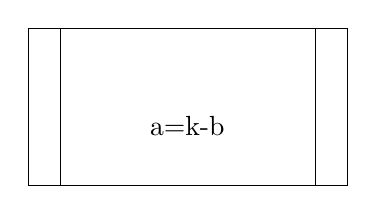
\begin{tikzpicture}
\pgftransformxscale{1.000000}
\pgftransformyscale{-1.000000}
\definecolor{dialinecolor}{rgb}{0.000000, 0.000000, 0.000000}
\pgfsetstrokecolor{dialinecolor}
\definecolor{dialinecolor}{rgb}{1.000000, 1.000000, 1.000000}
\pgfsetfillcolor{dialinecolor}
\pgfsetlinewidth{0.100000\du}
\pgfsetdash{}{0pt}
\pgfsetdash{}{0pt}
\pgfsetbuttcap
\pgfsetmiterjoin
\pgfsetlinewidth{0.100000\du}
\pgfsetbuttcap
\pgfsetmiterjoin
\pgfsetdash{}{0pt}
\definecolor{dialinecolor}{rgb}{1.000000, 1.000000, 1.000000}
\pgfsetfillcolor{dialinecolor}
\fill (5.000000\du,0.850000\du)--(5.000000\du,2.850000\du)--(9.050000\du,2.850000\du)--(9.050000\du,0.850000\du)--cycle;
\definecolor{dialinecolor}{rgb}{0.000000, 0.000000, 0.000000}
\pgfsetstrokecolor{dialinecolor}
\draw (5.000000\du,0.850000\du)--(5.000000\du,2.850000\du)--(9.050000\du,2.850000\du)--(9.050000\du,0.850000\du)--cycle;
\pgfsetbuttcap
\pgfsetmiterjoin
\pgfsetdash{}{0pt}
\definecolor{dialinecolor}{rgb}{0.000000, 0.000000, 0.000000}
\pgfsetstrokecolor{dialinecolor}
\draw (5.405000\du,0.850000\du)--(5.405000\du,2.850000\du);
\pgfsetbuttcap
\pgfsetmiterjoin
\pgfsetdash{}{0pt}
\definecolor{dialinecolor}{rgb}{0.000000, 0.000000, 0.000000}
\pgfsetstrokecolor{dialinecolor}
\draw (8.645000\du,0.850000\du)--(8.645000\du,2.850000\du);
% setfont left to latex
\definecolor{dialinecolor}{rgb}{0.000000, 0.000000, 0.000000}
\pgfsetstrokecolor{dialinecolor}
\node at (7.025000\du,2.100000\du){a=k-b};
\end{tikzpicture}
 & Символ відображає виконання процесу, що складається з однієї або декількох операцій, який визначений в іншому місці програми (в підпрограмі, модулі). \\
\hline
Дані & % Graphic for TeX using PGF
% Title: C:\Documents and Settings\Admin\Мои документы\Мои рисунки\Диаграмма1.dia
% Creator: Dia v0.97.2
% CreationDate: Sat Sep 08 10:40:01 2012
% For: Admin
% \usepackage{tikz}
% The following commands are not supported in PSTricks at present
% We define them conditionally, so when they are implemented,
% this pgf file will use them.
\ifx\du\undefined
  \newlength{\du}
\fi
\setlength{\du}{15\unitlength}
\begin{tikzpicture}
\pgftransformxscale{1.000000}
\pgftransformyscale{-1.000000}
\definecolor{dialinecolor}{rgb}{0.000000, 0.000000, 0.000000}
\pgfsetstrokecolor{dialinecolor}
\definecolor{dialinecolor}{rgb}{1.000000, 1.000000, 1.000000}
\pgfsetfillcolor{dialinecolor}
\definecolor{dialinecolor}{rgb}{1.000000, 1.000000, 1.000000}
\pgfsetfillcolor{dialinecolor}
\fill (5.818382\du,0.600000\du)--(8.950000\du,0.600000\du)--(8.222060\du,2.600000\du)--(5.090442\du,2.600000\du)--cycle;
\pgfsetlinewidth{0.100000\du}
\pgfsetdash{}{0pt}
\pgfsetdash{}{0pt}
\pgfsetmiterjoin
\definecolor{dialinecolor}{rgb}{0.000000, 0.000000, 0.000000}
\pgfsetstrokecolor{dialinecolor}
\draw (5.818382\du,0.600000\du)--(8.950000\du,0.600000\du)--(8.222060\du,2.600000\du)--(5.090442\du,2.600000\du)--cycle;
% setfont left to latex
\definecolor{dialinecolor}{rgb}{0.000000, 0.000000, 0.000000}
\pgfsetstrokecolor{dialinecolor}
\node at (7.020221\du,1.840000\du){x1, x2};
\end{tikzpicture}
 & Перетворення даних у форму, придатну для обробки (введення) або відображення результатів обробки (висновок). \\
\hline
Кордон циклу & % Graphic for TeX using PGF
% Title: C:\Documents and Settings\Admin\Мои документы\Мои рисунки\Диаграмма1.dia
% Creator: Dia v0.97.2
% CreationDate: Sat Sep 08 10:45:13 2012
% For: Admin
% \usepackage{tikz}
% The following commands are not supported in PSTricks at present
% We define them conditionally, so when they are implemented,
% this pgf file will use them.
\ifx\du\undefined
  \newlength{\du}
\fi
\setlength{\du}{15\unitlength}
\begin{tikzpicture}
\pgftransformxscale{1.000000}
\pgftransformyscale{-1.000000}
\definecolor{dialinecolor}{rgb}{0.000000, 0.000000, 0.000000}
\pgfsetstrokecolor{dialinecolor}
\definecolor{dialinecolor}{rgb}{1.000000, 1.000000, 1.000000}
\pgfsetfillcolor{dialinecolor}
\pgfsetlinewidth{0.100000\du}
\pgfsetdash{}{0pt}
\pgfsetdash{}{0pt}
\pgfsetbuttcap
\pgfsetmiterjoin
\pgfsetlinewidth{0.100000\du}
\pgfsetbuttcap
\pgfsetmiterjoin
\pgfsetdash{}{0pt}
\definecolor{dialinecolor}{rgb}{1.000000, 1.000000, 1.000000}
\pgfsetfillcolor{dialinecolor}
\pgfpathmoveto{\pgfpoint{5.479214\du}{0.850000\du}}
\pgfpathlineto{\pgfpoint{8.371536\du}{0.850000\du}}
\pgfpathlineto{\pgfpoint{8.950000\du}{1.625000\du}}
\pgfpathlineto{\pgfpoint{8.371536\du}{2.400000\du}}
\pgfpathlineto{\pgfpoint{5.479214\du}{2.400000\du}}
\pgfpathlineto{\pgfpoint{4.900750\du}{1.625000\du}}
\pgfpathlineto{\pgfpoint{5.479214\du}{0.850000\du}}
\pgfusepath{fill}
\definecolor{dialinecolor}{rgb}{0.000000, 0.000000, 0.000000}
\pgfsetstrokecolor{dialinecolor}
\pgfpathmoveto{\pgfpoint{5.479214\du}{0.850000\du}}
\pgfpathlineto{\pgfpoint{8.371536\du}{0.850000\du}}
\pgfpathlineto{\pgfpoint{8.950000\du}{1.625000\du}}
\pgfpathlineto{\pgfpoint{8.371536\du}{2.400000\du}}
\pgfpathlineto{\pgfpoint{5.479214\du}{2.400000\du}}
\pgfpathlineto{\pgfpoint{4.900750\du}{1.625000\du}}
\pgfpathlineto{\pgfpoint{5.479214\du}{0.850000\du}}
\pgfusepath{stroke}
% setfont left to latex
\definecolor{dialinecolor}{rgb}{0.000000, 0.000000, 0.000000}
\pgfsetstrokecolor{dialinecolor}
\node at (6.925375\du,1.875000\du){i=1;10;1};
\end{tikzpicture}
 & Символ складається з двох частин~--- відповідно, початок і кінець циклу - операції, що виконуються всередині циклу, розміщуються між ними. Умови циклу і збільшення записуються всередині символу початку або кінця циклу - в залежності від типу організації циклу. \\
\hline
З'єднувач & % Graphic for TeX using PGF
% Title: C:\Documents and Settings\Admin\Мои документы\Мои рисунки\Диаграмма1.dia
% Creator: Dia v0.97.2
% CreationDate: Sat Sep 08 10:46:12 2012
% For: Admin
% \usepackage{tikz}
% The following commands are not supported in PSTricks at present
% We define them conditionally, so when they are implemented,
% this pgf file will use them.
\ifx\du\undefined
  \newlength{\du}
\fi
\setlength{\du}{15\unitlength}
\begin{tikzpicture}
\pgftransformxscale{1.000000}
\pgftransformyscale{-1.000000}
\definecolor{dialinecolor}{rgb}{0.000000, 0.000000, 0.000000}
\pgfsetstrokecolor{dialinecolor}
\definecolor{dialinecolor}{rgb}{1.000000, 1.000000, 1.000000}
\pgfsetfillcolor{dialinecolor}
\definecolor{dialinecolor}{rgb}{1.000000, 1.000000, 1.000000}
\pgfsetfillcolor{dialinecolor}
\pgfpathellipse{\pgfpoint{6.147734\du}{1.633373\du}}{\pgfpoint{1.034541\du}{0\du}}{\pgfpoint{0\du}{0.961133\du}}
\pgfusepath{fill}
\pgfsetlinewidth{0.100000\du}
\pgfsetdash{}{0pt}
\pgfsetdash{}{0pt}
\pgfsetmiterjoin
\definecolor{dialinecolor}{rgb}{0.000000, 0.000000, 0.000000}
\pgfsetstrokecolor{dialinecolor}
\pgfpathellipse{\pgfpoint{6.147734\du}{1.633373\du}}{\pgfpoint{1.034541\du}{0\du}}{\pgfpoint{0\du}{0.961133\du}}
\pgfusepath{stroke}
% setfont left to latex
\definecolor{dialinecolor}{rgb}{0.000000, 0.000000, 0.000000}
\pgfsetstrokecolor{dialinecolor}
\node at (6.147734\du,1.873373\du){A};
\end{tikzpicture}
 & Символ відображає вхід в частину схеми і вихід з іншої частини цієї схеми.  \\
\hline
\end{longtable}

Приклад типової блок-схеми з вводом даних, розгалуженням, обчисленням та виводом даних дано на  малюнку~\ref{bl-ch:image}. 

\begin{figure}

\caption{Приклад нескладної блок-схеми}
% Graphic for TeX using PGF
% Title: C:\Documents and Settings\Admin\Мои документы\Мои рисунки\Диаграмма1.dia
% Creator: Dia v0.97.2
% CreationDate: Sat Sep 08 11:28:49 2012
% For: Admin
% \usepackage{tikz}
% The following commands are not supported in PSTricks at present
% We define them conditionally, so when they are implemented,
% this pgf file will use them.
\ifx\du\undefined
  \newlength{\du}
\fi
\setlength{\du}{15\unitlength}
\begin{tikzpicture}
\pgftransformxscale{1.000000}
\pgftransformyscale{-1.000000}
\definecolor{dialinecolor}{rgb}{0.000000, 0.000000, 0.000000}
\pgfsetstrokecolor{dialinecolor}
\definecolor{dialinecolor}{rgb}{1.000000, 1.000000, 1.000000}
\pgfsetfillcolor{dialinecolor}
\pgfsetlinewidth{0.100000\du}
\pgfsetdash{}{0pt}
\pgfsetdash{}{0pt}
\pgfsetbuttcap
\pgfsetmiterjoin
\pgfsetlinewidth{0.100000\du}
\pgfsetbuttcap
\pgfsetmiterjoin
\pgfsetdash{}{0pt}
\definecolor{dialinecolor}{rgb}{1.000000, 1.000000, 1.000000}
\pgfsetfillcolor{dialinecolor}
\pgfpathmoveto{\pgfpoint{4.983333\du}{0.725000\du}}
\pgfpathlineto{\pgfpoint{8.116667\du}{0.725000\du}}
\pgfpathcurveto{\pgfpoint{8.549290\du}{0.725000\du}}{\pgfpoint{8.900000\du}{1.004822\du}}{\pgfpoint{8.900000\du}{1.350000\du}}
\pgfpathcurveto{\pgfpoint{8.900000\du}{1.695178\du}}{\pgfpoint{8.549290\du}{1.975000\du}}{\pgfpoint{8.116667\du}{1.975000\du}}
\pgfpathlineto{\pgfpoint{4.983333\du}{1.975000\du}}
\pgfpathcurveto{\pgfpoint{4.550710\du}{1.975000\du}}{\pgfpoint{4.200000\du}{1.695178\du}}{\pgfpoint{4.200000\du}{1.350000\du}}
\pgfpathcurveto{\pgfpoint{4.200000\du}{1.004822\du}}{\pgfpoint{4.550710\du}{0.725000\du}}{\pgfpoint{4.983333\du}{0.725000\du}}
\pgfusepath{fill}
\definecolor{dialinecolor}{rgb}{0.000000, 0.000000, 0.000000}
\pgfsetstrokecolor{dialinecolor}
\pgfpathmoveto{\pgfpoint{4.983333\du}{0.725000\du}}
\pgfpathlineto{\pgfpoint{8.116667\du}{0.725000\du}}
\pgfpathcurveto{\pgfpoint{8.549290\du}{0.725000\du}}{\pgfpoint{8.900000\du}{1.004822\du}}{\pgfpoint{8.900000\du}{1.350000\du}}
\pgfpathcurveto{\pgfpoint{8.900000\du}{1.695178\du}}{\pgfpoint{8.549290\du}{1.975000\du}}{\pgfpoint{8.116667\du}{1.975000\du}}
\pgfpathlineto{\pgfpoint{4.983333\du}{1.975000\du}}
\pgfpathcurveto{\pgfpoint{4.550710\du}{1.975000\du}}{\pgfpoint{4.200000\du}{1.695178\du}}{\pgfpoint{4.200000\du}{1.350000\du}}
\pgfpathcurveto{\pgfpoint{4.200000\du}{1.004822\du}}{\pgfpoint{4.550710\du}{0.725000\du}}{\pgfpoint{4.983333\du}{0.725000\du}}
\pgfusepath{stroke}
% setfont left to latex
\definecolor{dialinecolor}{rgb}{0.000000, 0.000000, 0.000000}
\pgfsetstrokecolor{dialinecolor}
\node at (6.550000\du,1.600000\du){Початок};
\definecolor{dialinecolor}{rgb}{1.000000, 1.000000, 1.000000}
\pgfsetfillcolor{dialinecolor}
\fill (5.517353\du,3.325000\du)--(9.701029\du,3.325000\du)--(8.973089\du,5.325000\du)--(4.789413\du,5.325000\du)--cycle;
\pgfsetlinewidth{0.100000\du}
\pgfsetdash{}{0pt}
\pgfsetdash{}{0pt}
\pgfsetmiterjoin
\definecolor{dialinecolor}{rgb}{0.000000, 0.000000, 0.000000}
\pgfsetstrokecolor{dialinecolor}
\draw (5.517353\du,3.325000\du)--(9.701029\du,3.325000\du)--(8.973089\du,5.325000\du)--(4.789413\du,5.325000\du)--cycle;
% setfont left to latex
\definecolor{dialinecolor}{rgb}{0.000000, 0.000000, 0.000000}
\pgfsetstrokecolor{dialinecolor}
\node at (7.245221\du,4.565000\du){x1, x2, x3};
\definecolor{dialinecolor}{rgb}{1.000000, 1.000000, 1.000000}
\pgfsetfillcolor{dialinecolor}
\fill (6.869670\du,6.850000\du)--(9.985382\du,8.301957\du)--(6.869670\du,9.753914\du)--(3.753958\du,8.301957\du)--cycle;
\pgfsetlinewidth{0.100000\du}
\pgfsetdash{}{0pt}
\pgfsetdash{}{0pt}
\pgfsetmiterjoin
\definecolor{dialinecolor}{rgb}{0.000000, 0.000000, 0.000000}
\pgfsetstrokecolor{dialinecolor}
\draw (6.869670\du,6.850000\du)--(9.985382\du,8.301957\du)--(6.869670\du,9.753914\du)--(3.753958\du,8.301957\du)--cycle;
% setfont left to latex
\definecolor{dialinecolor}{rgb}{0.000000, 0.000000, 0.000000}
\pgfsetstrokecolor{dialinecolor}
\node at (6.869670\du,8.541957\du){x1<x2};
% setfont left to latex
\definecolor{dialinecolor}{rgb}{0.000000, 0.000000, 0.000000}
\pgfsetstrokecolor{dialinecolor}
\node[anchor=west] at (2.725000\du,7.725000\du){Так};
% setfont left to latex
\definecolor{dialinecolor}{rgb}{0.000000, 0.000000, 0.000000}
\pgfsetstrokecolor{dialinecolor}
\node[anchor=west] at (10.150000\du,7.750000\du){Ні};
\definecolor{dialinecolor}{rgb}{1.000000, 1.000000, 1.000000}
\pgfsetfillcolor{dialinecolor}
\fill (1.066250\du,10.050000\du)--(1.066250\du,12.000000\du)--(5.333750\du,12.000000\du)--(5.333750\du,10.050000\du)--cycle;
\pgfsetlinewidth{0.100000\du}
\pgfsetdash{}{0pt}
\pgfsetdash{}{0pt}
\pgfsetmiterjoin
\definecolor{dialinecolor}{rgb}{0.000000, 0.000000, 0.000000}
\pgfsetstrokecolor{dialinecolor}
\draw (1.066250\du,10.050000\du)--(1.066250\du,12.000000\du)--(5.333750\du,12.000000\du)--(5.333750\du,10.050000\du)--cycle;
% setfont left to latex
\definecolor{dialinecolor}{rgb}{0.000000, 0.000000, 0.000000}
\pgfsetstrokecolor{dialinecolor}
\node at (3.200000\du,11.265000\du){a = x1 - x3};
\definecolor{dialinecolor}{rgb}{1.000000, 1.000000, 1.000000}
\pgfsetfillcolor{dialinecolor}
\fill (9.000000\du,10.090000\du)--(9.000000\du,11.990000\du)--(13.678750\du,11.990000\du)--(13.678750\du,10.090000\du)--cycle;
\pgfsetlinewidth{0.100000\du}
\pgfsetdash{}{0pt}
\pgfsetdash{}{0pt}
\pgfsetmiterjoin
\definecolor{dialinecolor}{rgb}{0.000000, 0.000000, 0.000000}
\pgfsetstrokecolor{dialinecolor}
\draw (9.000000\du,10.090000\du)--(9.000000\du,11.990000\du)--(13.678750\du,11.990000\du)--(13.678750\du,10.090000\du)--cycle;
% setfont left to latex
\definecolor{dialinecolor}{rgb}{0.000000, 0.000000, 0.000000}
\pgfsetstrokecolor{dialinecolor}
\node at (11.339375\du,11.280000\du){a = x1 + x3};
\pgfsetlinewidth{0.100000\du}
\pgfsetdash{}{0pt}
\pgfsetdash{}{0pt}
\pgfsetbuttcap
\pgfsetmiterjoin
\pgfsetlinewidth{0.100000\du}
\pgfsetbuttcap
\pgfsetmiterjoin
\pgfsetdash{}{0pt}
\definecolor{dialinecolor}{rgb}{1.000000, 1.000000, 1.000000}
\pgfsetfillcolor{dialinecolor}
\fill (6.350000\du,13.950000\du)--(8.350000\du,13.950000\du)--(7.350000\du,16.150000\du)--cycle;
\definecolor{dialinecolor}{rgb}{0.000000, 0.000000, 0.000000}
\pgfsetstrokecolor{dialinecolor}
\draw (6.350000\du,13.950000\du)--(8.350000\du,13.950000\du)--(7.350000\du,16.150000\du)--cycle;
% setfont left to latex
\definecolor{dialinecolor}{rgb}{0.000000, 0.000000, 0.000000}
\pgfsetstrokecolor{dialinecolor}
\node at (7.350000\du,14.750000\du){};
\pgfsetlinewidth{0.100000\du}
\pgfsetdash{}{0pt}
\pgfsetdash{}{0pt}
\pgfsetbuttcap
\pgfsetmiterjoin
\pgfsetlinewidth{0.100000\du}
\pgfsetbuttcap
\pgfsetmiterjoin
\pgfsetdash{}{0pt}
\definecolor{dialinecolor}{rgb}{1.000000, 1.000000, 1.000000}
\pgfsetfillcolor{dialinecolor}
\pgfpathmoveto{\pgfpoint{6.128333\du}{20.940000\du}}
\pgfpathlineto{\pgfpoint{9.261667\du}{20.940000\du}}
\pgfpathcurveto{\pgfpoint{9.694290\du}{20.940000\du}}{\pgfpoint{10.045000\du}{21.219822\du}}{\pgfpoint{10.045000\du}{21.565000\du}}
\pgfpathcurveto{\pgfpoint{10.045000\du}{21.910178\du}}{\pgfpoint{9.694290\du}{22.190000\du}}{\pgfpoint{9.261667\du}{22.190000\du}}
\pgfpathlineto{\pgfpoint{6.128333\du}{22.190000\du}}
\pgfpathcurveto{\pgfpoint{5.695710\du}{22.190000\du}}{\pgfpoint{5.345000\du}{21.910178\du}}{\pgfpoint{5.345000\du}{21.565000\du}}
\pgfpathcurveto{\pgfpoint{5.345000\du}{21.219822\du}}{\pgfpoint{5.695710\du}{20.940000\du}}{\pgfpoint{6.128333\du}{20.940000\du}}
\pgfusepath{fill}
\definecolor{dialinecolor}{rgb}{0.000000, 0.000000, 0.000000}
\pgfsetstrokecolor{dialinecolor}
\pgfpathmoveto{\pgfpoint{6.128333\du}{20.940000\du}}
\pgfpathlineto{\pgfpoint{9.261667\du}{20.940000\du}}
\pgfpathcurveto{\pgfpoint{9.694290\du}{20.940000\du}}{\pgfpoint{10.045000\du}{21.219822\du}}{\pgfpoint{10.045000\du}{21.565000\du}}
\pgfpathcurveto{\pgfpoint{10.045000\du}{21.910178\du}}{\pgfpoint{9.694290\du}{22.190000\du}}{\pgfpoint{9.261667\du}{22.190000\du}}
\pgfpathlineto{\pgfpoint{6.128333\du}{22.190000\du}}
\pgfpathcurveto{\pgfpoint{5.695710\du}{22.190000\du}}{\pgfpoint{5.345000\du}{21.910178\du}}{\pgfpoint{5.345000\du}{21.565000\du}}
\pgfpathcurveto{\pgfpoint{5.345000\du}{21.219822\du}}{\pgfpoint{5.695710\du}{20.940000\du}}{\pgfpoint{6.128333\du}{20.940000\du}}
\pgfusepath{stroke}
% setfont left to latex
\definecolor{dialinecolor}{rgb}{0.000000, 0.000000, 0.000000}
\pgfsetstrokecolor{dialinecolor}
\node at (7.695000\du,21.815000\du){Початок};
\definecolor{dialinecolor}{rgb}{1.000000, 1.000000, 1.000000}
\pgfsetfillcolor{dialinecolor}
\fill (6.322940\du,17.390000\du)--(10.506617\du,17.390000\du)--(9.778676\du,19.390000\du)--(5.595000\du,19.390000\du)--cycle;
\pgfsetlinewidth{0.100000\du}
\pgfsetdash{}{0pt}
\pgfsetdash{}{0pt}
\pgfsetmiterjoin
\definecolor{dialinecolor}{rgb}{0.000000, 0.000000, 0.000000}
\pgfsetstrokecolor{dialinecolor}
\draw (6.322940\du,17.390000\du)--(10.506617\du,17.390000\du)--(9.778676\du,19.390000\du)--(5.595000\du,19.390000\du)--cycle;
% setfont left to latex
\definecolor{dialinecolor}{rgb}{0.000000, 0.000000, 0.000000}
\pgfsetstrokecolor{dialinecolor}
\node at (8.050808\du,18.630000\du){a};
\pgfsetlinewidth{0.100000\du}
\pgfsetdash{}{0pt}
\pgfsetdash{}{0pt}
\pgfsetmiterjoin
\pgfsetbuttcap
{
\definecolor{dialinecolor}{rgb}{0.000000, 0.000000, 0.000000}
\pgfsetfillcolor{dialinecolor}
% was here!!!
\pgfsetarrowsend{stealth}
{\pgfsetcornersarced{\pgfpoint{0.000000\du}{0.000000\du}}\definecolor{dialinecolor}{rgb}{0.000000, 0.000000, 0.000000}
\pgfsetstrokecolor{dialinecolor}
\draw (3.753958\du,8.301957\du)--(3.753958\du,8.300000\du)--(3.200000\du,8.300000\du)--(3.200000\du,10.050000\du);
}}
\pgfsetlinewidth{0.100000\du}
\pgfsetdash{}{0pt}
\pgfsetdash{}{0pt}
\pgfsetmiterjoin
\pgfsetbuttcap
{
\definecolor{dialinecolor}{rgb}{0.000000, 0.000000, 0.000000}
\pgfsetfillcolor{dialinecolor}
% was here!!!
\pgfsetarrowsend{stealth}
{\pgfsetcornersarced{\pgfpoint{0.000000\du}{0.000000\du}}\definecolor{dialinecolor}{rgb}{0.000000, 0.000000, 0.000000}
\pgfsetstrokecolor{dialinecolor}
\draw (9.985382\du,8.301957\du)--(9.985382\du,8.300000\du)--(11.339375\du,8.300000\du)--(11.339375\du,10.090000\du);
}}
\pgfsetlinewidth{0.100000\du}
\pgfsetdash{}{0pt}
\pgfsetdash{}{0pt}
\pgfsetmiterjoin
\pgfsetbuttcap
{
\definecolor{dialinecolor}{rgb}{0.000000, 0.000000, 0.000000}
\pgfsetfillcolor{dialinecolor}
% was here!!!
\pgfsetarrowsend{stealth}
{\pgfsetcornersarced{\pgfpoint{0.000000\du}{0.000000\du}}\definecolor{dialinecolor}{rgb}{0.000000, 0.000000, 0.000000}
\pgfsetstrokecolor{dialinecolor}
\draw (3.200000\du,12.000000\du)--(3.200000\du,12.975000\du)--(6.850000\du,12.975000\du)--(6.850000\du,13.950000\du);
}}
\pgfsetlinewidth{0.100000\du}
\pgfsetdash{}{0pt}
\pgfsetdash{}{0pt}
\pgfsetmiterjoin
\pgfsetbuttcap
{
\definecolor{dialinecolor}{rgb}{0.000000, 0.000000, 0.000000}
\pgfsetfillcolor{dialinecolor}
% was here!!!
\pgfsetarrowsend{stealth}
{\pgfsetcornersarced{\pgfpoint{0.000000\du}{0.000000\du}}\definecolor{dialinecolor}{rgb}{0.000000, 0.000000, 0.000000}
\pgfsetstrokecolor{dialinecolor}
\draw (11.339375\du,11.990000\du)--(11.339375\du,12.970000\du)--(7.850000\du,12.970000\du)--(7.850000\du,13.950000\du);
}}
\pgfsetlinewidth{0.100000\du}
\pgfsetdash{}{0pt}
\pgfsetdash{}{0pt}
\pgfsetbuttcap
{
\definecolor{dialinecolor}{rgb}{0.000000, 0.000000, 0.000000}
\pgfsetfillcolor{dialinecolor}
% was here!!!
\pgfsetarrowsend{stealth}
\definecolor{dialinecolor}{rgb}{0.000000, 0.000000, 0.000000}
\pgfsetstrokecolor{dialinecolor}
\draw (6.550000\du,1.975000\du)--(6.563272\du,3.325000\du);
}
\pgfsetlinewidth{0.100000\du}
\pgfsetdash{}{0pt}
\pgfsetdash{}{0pt}
\pgfsetbuttcap
{
\definecolor{dialinecolor}{rgb}{0.000000, 0.000000, 0.000000}
\pgfsetfillcolor{dialinecolor}
% was here!!!
\pgfsetarrowsend{stealth}
\definecolor{dialinecolor}{rgb}{0.000000, 0.000000, 0.000000}
\pgfsetstrokecolor{dialinecolor}
\draw (6.881251\du,5.325000\du)--(6.869670\du,6.850000\du);
}
\pgfsetlinewidth{0.100000\du}
\pgfsetdash{}{0pt}
\pgfsetdash{}{0pt}
\pgfsetbuttcap
{
\definecolor{dialinecolor}{rgb}{0.000000, 0.000000, 0.000000}
\pgfsetfillcolor{dialinecolor}
% was here!!!
\pgfsetarrowsend{stealth}
\definecolor{dialinecolor}{rgb}{0.000000, 0.000000, 0.000000}
\pgfsetstrokecolor{dialinecolor}
\draw (7.350000\du,16.150000\du)--(7.368860\du,17.390000\du);
}
\pgfsetlinewidth{0.100000\du}
\pgfsetdash{}{0pt}
\pgfsetdash{}{0pt}
\pgfsetbuttcap
{
\definecolor{dialinecolor}{rgb}{0.000000, 0.000000, 0.000000}
\pgfsetfillcolor{dialinecolor}
% was here!!!
\pgfsetarrowsend{stealth}
\definecolor{dialinecolor}{rgb}{0.000000, 0.000000, 0.000000}
\pgfsetstrokecolor{dialinecolor}
\draw (7.686838\du,19.390000\du)--(7.695000\du,20.940000\du);
}
\end{tikzpicture}

\label{bl-ch:image}
\end{figure} 


\section{Оформлення програмного коду}
Програмний код необхідно оформлювати у друкованому вигляді, бажано використовуючи моноширинний шрифт \verb'Сourier' або \verb'Сourier New' розміром 12~--~14pt. Приклад оформлення лістингів надано нижче.
\section{Оформлення скріншотів}
Скріншоти HTML-форм або PHP-сценаріїв бажано оформлювати без рамки веб-браузера по 1~--~2 зображення на сторінку. При використанні на фоні HTML-сторінки темних кольорів можливе редагування зображення з метою висвітлення кольорів. Приклад зображення, що отримано з комбінацій клавіш \verb'Alt+PrtCs' зображена на малюнку~\ref{prsc-orig:image}, та бажане зображення на малюнку малюнку~\ref{prsc-rel:image}. Небажане оформлення скріншота дано на  малюнку~\ref{prsc-bad:image}.

\begin{figure}
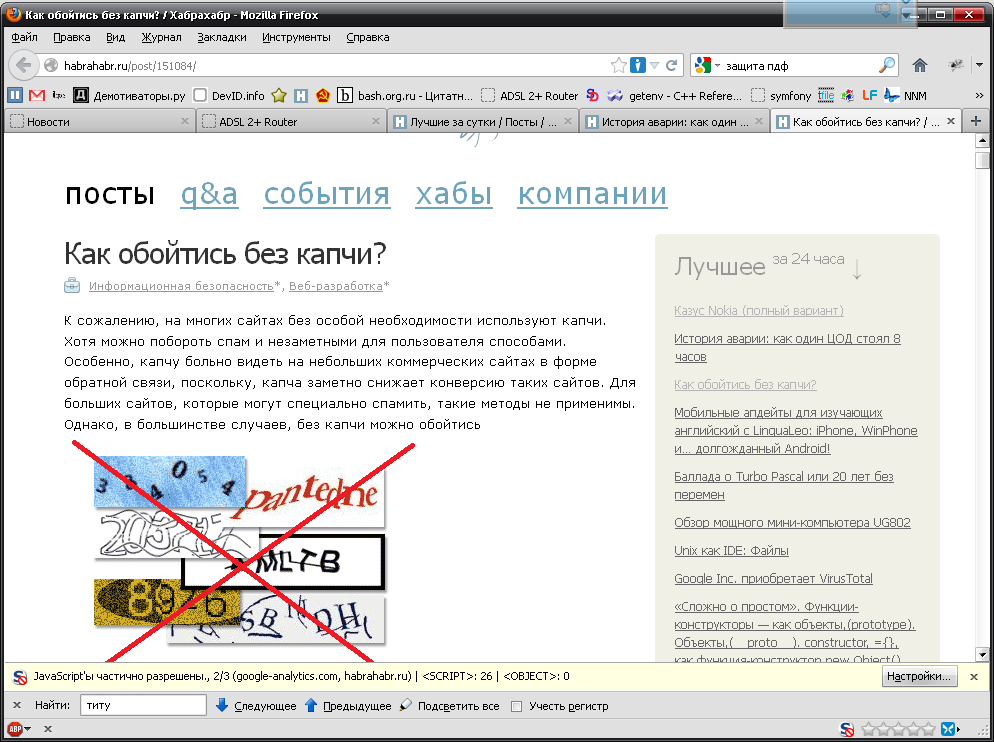
\includegraphics[scale=1,width=10cm]{ap01-09.png}
\caption{Оригінал зображення}
\label{prsc-orig:image}
\end{figure}


\begin{figure}
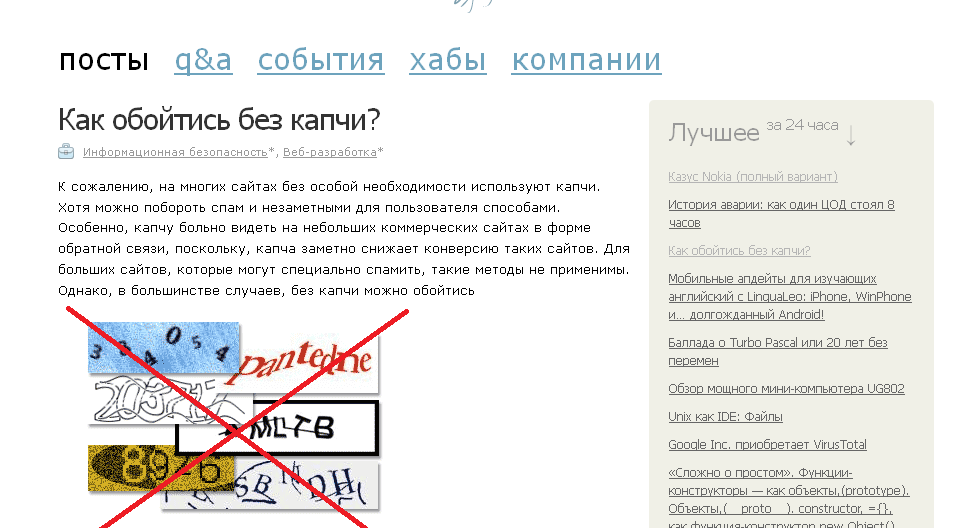
\includegraphics[scale=1,width=10cm]{ap01-10.png}
\caption{Оброблене зображення}
\label{prsc-rel:image}
\end{figure}

\begin{figure}
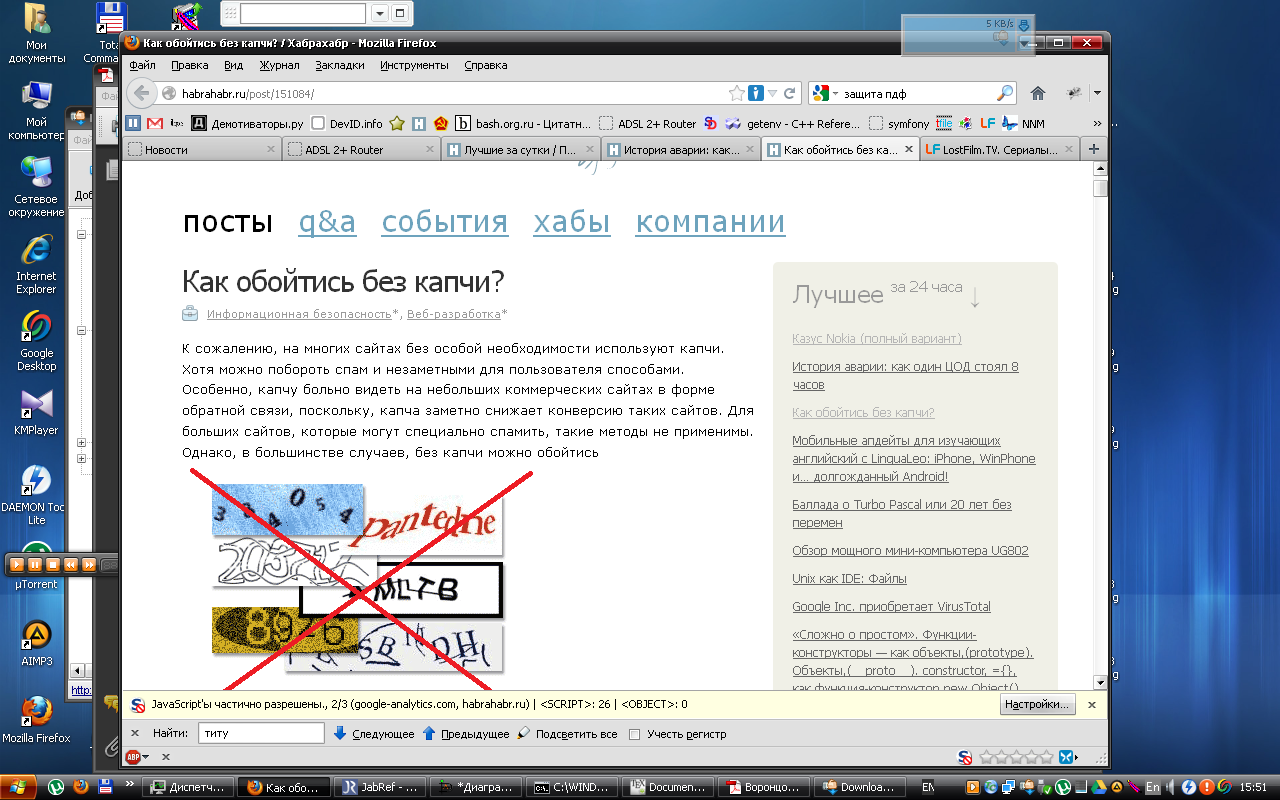
\includegraphics[scale=1,width=10cm]{ap01-11.png}
\caption{Необроблене зображення}
\label{prsc-bad:image}
\end{figure}
\chapter{Матеріали до Л/Р \No 2}
\section{Елементи форм HTML}
\index{HTML!форми}
\subsection{INPUT і його методи}
\index{HTML!форми!input}
\label{inp-tag:app}
\subsection*{Однорядкові поля введення даних}

\begin{verbatim}
<input type=text name=им'я_параметра [value=значення] 
[size=розмір_поля] [maxlen=довжина_поля]>
\end{verbatim}

Даний тег створює поле вводу з максимально допустимою довжиною тексту <<maxlen>> і розміром в size <<знакомест>>. Якщо вказаний атрибут <<value>>, то в поле буде спочатку відображатися значення даного атрибуту. У квадратних дужках \verb'[]' позначені необов'язкові атрибути.

\subsection*{Поля вводу паролів}

\begin{verbatim}
<input type=password name=им'я_параметра [value=значення] 
[size=розмір_поля] [maxlen=довжина_поля]>
\end{verbatim}

Структура даного тегу така сама як і у <input type=text>. Різниця лише у відображенні даних, що вводить користувач.


\subsection*{Приховане текстове поле}

\begin{verbatim}
<input type=hidden name=им'я_параметра [value=значення]>
\end{verbatim}

Такі поля передають дані серверу, але не відображаються на сторінці. Значення атрибуту <<value>> встановлюється при формуванні сторінки, або JavaScript-сценарієм.

\subsection*{Незалежні перемикачі}

\begin{verbatim}
<input type=checkbox name=им'я_параметра [value=значення]
[checked]>
\end{verbatim} 

Перемикач виду <<прапорець>>. У разі встановлення прапорця при відправлені форми серверу будуть передані параметри <<им'я\_параметра=значення>>. Якщо прапорець не встановлено серверу взагалі нічого не буде відправлено. 

Перемикач за замовчуванням вимкнутий, щоб зробити його увімкнутим за замовчуванням треба встановити атрибут  <<checked>>.

Стан перемикача не залежить від стану інших перемикачів цього типу.

\subsection*{Залежні перемикачі}

Залежний перемикач, так само як і незалежний перемикач, може заходитись у двох станах, в залежності від атрибуту  <<checked>>. При цьому на формі може бути увімкнений лише один перемикач серед групи перемикачів з однаковим атрибутом <<name>>.
\begin{verbatim}
<form action="http://localhost/script.php" method="GET">
<input type=radio name=answer value=yes checked>Да
<input type=radio name=answer value=no>Нет
<input type=submit value=Отправить>
</form>
\end{verbatim}

\subsection*{Кнопки відправлення та очищення параметрів форми}

Кнопка відправки служить для передачі серверу змісту форми на сторінці. Атрибут <<value>> визначає текст, ща відображається на кнопці. Під час відправлення форми серверу будуть передані дані кнопки у вигляді <<им'я\_параметра=значення>>.
\begin{verbatim}
<input type=submit [name=им'я_параметра] value=значення>
\end{verbatim}
У разі використання кнопки із зображенням сереру передадуться координати кліку відносно зображення.
\begin{verbatim}
<input type=submit [name=им'я_параметра] src=зображення>
\end{verbatim}
Кнопка очищення форми знищує всі зміни внесені користувачем сайту у дану форму.
\begin{verbatim}
<input type=reset [name=им'я_параметра] value=значення>
\end{verbatim}

\subsection*{Поле вибору файлу}

Тег <input> також дозволяє активувати діалогове вікно вибору файлу та завантажувати його на сервер при відправленні форми.
\begin{verbatim}
<input type=file name=имя [value=имя_файла]>
\end{verbatim}


\subsection{Багаторядкове текстове поле}
\index{HTML!форми!textarea}
\label{tar-tag:app}
Синтаксис багаторядкового поля виглядає наступним чином:
\begin{verbatim}
<textarea name=имя [cols=ширина_в_символах] 
[rows=высота_в_символах] wrap=тип_переноса>
текст за замовчуванням
</textarea>
\end{verbatim}
Хоча висота і ширина поля необов'язкові параметри їх бажано вказувати. Атрибут <<wrap>> відповідає за перенос і може приймати наступні значення:
\begin{enumerate}
\item Virtual --- справа від тексту з'являється полоса прокрутки, а текст розбивається на рядки.
\item Physical --- залежить від браузера і виглядає по-різному
\item None --- текст залишається у тому вигляді, в якому користувач його ввів, з'являються горизонтальна і вертикальна полоси прокрутки.
\end{enumerate}

\subsection{Списки з вибором} \label{sel-tag:app}
\index{HTML!форми!select}
\subsection*{Списки з одиночним вибором}
\label{sel-tag:app}
Списки з одиночним вибором реалізуються за допомогою наступної конструкції:
\begin{verbatim}

<select name=day size=1>
<option value=1>Понедельник</option>
<option value=2>Вторник</option>
<option value=3 selected>Среда</option>
<option value=4>Четверг</option>
<option value=5>Пятница</option>
<option value=6>Суббота</option>
<option value=7>Воскресенье</option>
</select>

\end{verbatim}
При відправленні форми сервер отримає дані виду <<им'я\_параметра=значення>>. За замовчуванням може бути обраний пункт списку серед атрибутів якого є \verb'selected'.

\subsection*{Списки з множинним вибором}
Список з множинним вибором відрізняється лише атрибутом \verb'multiple' в середині тега \verb'<select>'.
\begin{verbatim}

<select name=day size=7 multiple>
<option value=1>Понедельник</option>
<option value=1>Вторник</option>
<option value=1>Среда</option>
<option value=1>Четверг</option>
<option value=1>Пятница</option>
<option value=1>Суббота</option>
<option value=1>Воскресенье</option>
</select>


\end{verbatim}


\section{Змінні-функції}
\index{PHP!функції!змінні-функції}
\label{var-func:app}
Приклад використання змінної-функції:
\begin{verbatim}
<?php
?php
function foo() {
    echo "In foo()<br />\n";
}
function bar($arg = '')
{
    echo "In bar(); argument was '$arg'.<br />\n";
}
// Функция-обертка для echo
function echoit($string)
{
    echo $string;
}

$func = 'foo';
$func();        // Вызывает функцию foo()
$func = 'bar';
$func('test');  // Вызывает функцию bar()
$func = 'echoit';
$func('test');  // Вызывает функцию echoit()
\end{verbatim}
\chapter{Матеріали до Л/Р \No 3}

\section{Змінні оточення web-сервера Apache}
\label{var-apa:app}
\nopagebreak[4]
\index{Web-сервери!Apache!змінні оточення}
\subsection{Формовані сервером змінні}

\textbf{AUTH\_TYPE} Використовується схема аутентифікації. Зазвичай BASIC

\textbf{CONTENT\_LENGTH} Довжина вмісту

\textbf{CONTENT\_TYPE} MIME-тип вмісту

\textbf{GETAWAY\_INTERFACE} Версія CGI, наприклад CGI/1.1

\textbf{PATH\_info} HTTP-шлях до сценарію

\textbf{PATH\_TRANSLATED} Повний шлях до сценарію

\textbf{REMOTE\_ADDR} IP-адреса запитуваного комп'ютера-клієнта

\textbf{REMOTE\_HOST} Доменне ім'я запитувача комп'ютера (якщо доступно). Доменне ім'я визначається веб-сервером за допомогою служби DNS. Директива \verb'HostnameLookups' сервера Apache дозволяє (або забороняє) перетворення IP-адреси в доменне ім'я.

\textbf{REMOTE\_PORT} Порт, закріплений за браузером для отримання відповіді від сервера

\textbf{REMOTE\_USER} Ім'я користувача, що пройшов аутентифікацію

\textbf{QUERY\_STRING} Рядок переданих серверу параметрів

\textbf{SERVER\_ADDR} IP-адресу сервера

\textbf{SERVER\_NAME} Доменне ім'я сервера. Визначається директивою ServerName файлу конфігурації

\textbf{SERVER\_PORT} TCP-порт Web-сервера. Зазвичай 80

\textbf{SERVER\_PROTOCOL} Версія протоколу HTTP. Наприклад, HTTP/1.1

\textbf{SERVER\_SOFTWARE} Програмне забезпечення сервера

\textbf{SCRIPT\_NAME} HTTP-шлях до сценарію

\textbf{SCRIPT\_FILENAME} Файл сценарію в файловій системі сервера (фізичний шлях). Наприклад, \verb'/var/www/cgi-bin/script.cgi'


\subsection{Спеціальні змінні сервера Apache}

\textbf{DOCUMENT\_ROOT} Фізичний шлях до кореневого WWW-каталогу сервера. Наприклад, \verb'/var/www.html/'

\textbf{SERVER\_ADMIN} Адреса електронної пошти адміністратора сервера

\textbf{SERVER\_SIGNATURE} Підпис сервера. Наприклад, <<\verb'Apache/1.3.3 сервера на www.somefirm.com порт 80'>>


\subsection{Змінні HTTP-полів запиту}

\textbf{HTTP\_HOST} Ім'я віртуального хоста, якому адресовано запит

\textbf{HTTP\_USER\_AGENT} Програмне забезпечення віддаленого користувача. Зазвичай ця змінна оточення містить назву і версію браузера

\textbf{HTTP\_ACCEPT} Список підтримуваних клієнтом типів інформації. 

\textbf{HTTP\_ACCEPT\_LANGUAGE} Список підтримуваних мов в порядку переваги, наприклад, RU, EN

\textbf{HTTP\_ACCEPT\_ENCODING} Список підтримуваних методів стиснення

\textbf{HTTP\_ACCEPT\_CHARSET} Список підтримуваних кодувань

\textbf{HTTP\_CONNECTION} Тип з'єднання. Можливі два варіанти:
\begin{list}{•}{•}
\item \verb'Keep-Alive'~--- якщо після відповіді на запит не потрібно розривати з'єднання;
\item \verb'Close'~--- якщо потрібно закрити з'єднання відразу після відповіді на запит.
\end{list}

\textbf{HTTP\_REFERER} Значення поля \verb'REFERER'. У цьому полі браузер передає URL ресурсу, який посилається на наш сервер. Наприклад, якщо користувач перейшов на сайт зі сторінки http://www.somehost.com/page.php, то значення поля \verb'REFERER' буде http://www.somehost.com/page.php.

\textbf{HTTP\_X\_FORWARDED\_FOR} Якщо користувач працює через проксі-сервер, то в цьому полі буде IP-адреса комп'ютера, який звернувся до проксі-сервера. Якщо це поле вже містить значення, то нове значення буде додано через кому.



\subsection{Суперглобальні масиви PHP}
\index{PHP!змінні!суперглобальні масиви}
\label{sup-glob:app}

\textbf{\$GLOBALS}~--- масив всіх глобальних змінних (у тому числі і для користувача).

\textbf{\$\_SERVER}~--- містить безліч інформації про поточний запит і сервер.

\textbf{\$\_ENV}~--- поточні змінні середовища. Їх набір специфічний для кожної конкретної платформи, на якій виконується сценарій.

\textbf{\$\_GET}~--- асоціативний масив з параметрами GET-запиту. У початковому вигляді ці параметри доступні в \verb|$_SERVER ['QUERY\_STRING']| і в \verb|$_SERVER ['REQUEST_URI']| в складі URI.

\textbf{\$\_POST}~--- асоціативний масив значень полів HTML-форми при відправки методом POST.

\textbf{\$\_FILES}~--- асоціативний масив з відомостями про надіслані методом POST файлах. Кожен елемент має індекс ідентичний значенню атрибута \verb'name' у формі і, в свою чергу, також є масивом з наступними елементами:
\begin{enumerate}
\item \verb|$_FILES['name']|~--- вихідне ім'я файлу на комп'ютері користувача.
\item \verb|$_FILES['type']|~--- зазначений агентом користувача MIME~--- тип файлу.
\item \verb|$_FILES['size']|~--- розмір файлу в байтах.
\item \verb|$_FILES['tmp_name']|~--- повний шлях до файлу в тимчасовій папці.
\item \verb|$_FILES['error']|~--- код помилки.
\end{enumerate}

\textbf{\$\_COOKIE}~--- асоціативний масив з переданими агентом користувача значеннями cookie.

\textbf{\$\_REQUEST}~--- загальний масив ввідних даних запиту користувача як в масивах \verb'$_GET, $_POST, $_COOKIE'. Починаючи з версії PHP 4.1 включається і вміст \verb'$_FILES'.


\section{Пріоритети виконання операторів}
\index{PHP!оператори!пріоритети}


\begin{center}
\begin{longtable}[t]{|c|p{25em}|}
\caption{Пріоритети виконання операторів} \label{pr-op:table}\\
\hline

Асоціативність & Оператор \\
\hline \endfirsthead
\caption*{\space Продовження} \\
\hline
Асоціативність & Оператор \\
\hline \endhead
\hline \endfoot
неасоціативна	& \verb|new| \\
права	& \verb|[|\\
неасоціативна	& \verb|++ --| \\
неасоціативна	& \verb|! ~ -(int) (float) (string) (array) (object) @| \\
ліва	& \verb|* / %| \\
ліва	& \verb|+ - .| \\
ліва	& \verb|<< >>| \\
неассоціативна	& \verb|< <= > >=| \\
неассоціативна	& \verb|== != === !==| \\
ліва	& \verb|&| \\
ліва	& \verb|^| \\
ліва	& \verb'|' \\
ліва	& \verb|&&| \\
ліва	& \verb'||' \\
ліва	& \verb|? :| \\
права	& \verb'= += -= *= /= .= %= &= |= ^= <<= >>='  \\
\penalty -10000
ліва	& \verb|and| \\
ліва	& \verb|xor| \\
ліва	& \verb|or| \\
ліва	& \verb|,| \\

\hline
\end{longtable}
\end{center}
\chapter{Матеріали до Л/Р \No 4}

\section{Рядки та регулярні вирази}
\subsection{Функції роботи з рядками}
\label{str-func:app}
\nopagebreak[4]


\index{PHP!змінні!рядки!функції}
\begin{longtable}[t]{|l|p{21em}|}

\caption{\space Повний список функцій роботи з рядками} \label{str-func:table}\\
\hline

Функція & Опис \\
\hline \endfirsthead
\caption*{\space Продовження} \\
\hline
Функція & Опис \\
\hline \endhead
\hline \endfoot
addcslashes & екрануючі спецсимволи в стилі мови C \\
addslashes & екрануючі спецсимволи в рядку \\
bin2hex & Перетворює бінарні дані у шістнадцятірічне подання \\
chr & Повертає символ за його кодом \\
chunk\_split & Розбиває рядок на фрагменти \\
convert\_cyr\_string & Перетворює рядок з одного кириличної кодування в інше \\
count\_chars & Повертає інформацію про символи, що входять в рядок \\
crc32 & Обчислює CRC32 для рядка \\
crypt & Необоротне шифрування (хешування) \\
echo & Виводить одну чи більше рядків \\
explode & Розбиває рядок на підрядки \\
fprintf & Записує отформатированную рядок у потік \\
get\_html\_translation\_table & Повертає таблицю перетворень \\
hebrev & Перетворює текст на івриті з логічного кодування у візуальне \\
hebrevc & Перетворює текст на івриті з логічнго кодування у візуальне з перетворенням в переклад \\
htmlentities & Перетворює символи у відповідні HTML теги \\
htmlspecialchars & Перетворює спеціальні символи в HTML теги \\
html\_entity\_decode & Перетворює HTML теги в відповідні символи \\
implode & Об'єднує елементи масиву в рядок \\
localeconv & Повертає інформацію про числові формати \\
ltrim & Видаляє пробіли з початку рядка \\
md5 & Повертає MD5-хеш рядка \\
md5\_file & Повертає MD5-хеш файлу \\
metaphone & Повертає ключ metaphone для рядка \\
nl2br & Вставляє HTML-код розриву рядка перед кожним переведенням рядка \\
number\_format & Форматує число з поділом груп \\
ord & Повертає ASCII-код символу \\
parse\_str & Розбирає рядок у змінні \\
print & Виводить рядок \\
printf & Виводить відформатований рядок \\
quoted\_printable\_decode & розкодує рядок, закодовану методом quoted printable \\
quotemeta & екрануючі спеціальні символи \\
rtrim & Видаляє пробіли з кінця рядка \\
sha1 & Повертає SHA1-хеш рядка \\
sha1\_file & Повертає SHA1-хеш файлу \\
similar\_text & Обчислює ступінь схожості двох рядків \\
soundex & Повертає ключ soundex для рядка \\
sprintf & Повертає відформатований рядок \\
sscanf & Розбирає рядок у відповідності із заданим форматом \\
strcasecmp & Порівняння рядків без урахування регістра, безпечне для даних у двійковій формі \\
strcmp & Порівняння рядків, безпечне для даних у двійковій формі \\
strcoll & Порівняння рядків з урахуванням поточної локалі \\
strcspn & Повертає довжину ділянки на початку рядка, не відповідного  масці \\
stripcslashes & Видаляє екранування символів, вироблене функцією addcslashes () \\
stripos & Повертає позицію першого входження підрядка без урахування регістра \\
stripslashes & Видаляє екранування символів, вироблене функцією addslashes () \\
strip\_tags & Видаляє HTML і PHP теги з рядка \\
stristr & Аналог функції strstr, але незалежний від регістру \\
strlen & Повертає довжину рядка \\
strnatcasecmp & Порівняння рядків без урахування регістра з використанням алгоритму \\
strnatcmp & Порівняння рядків з використанням алгоритму "природнього упорядкування" \\
strncasecmp & порівняння перших n символів рядків без урахування регістра, безпечне для даних у двійковій формі \\
strncmp & порівняння перших n символів рядків без урахування регістра, безпечне для даних у двійковій формі \\
strpos & Знаходить перше входження підрядка в рядок \\
strrchr & Знаходить останнє входження символу в рядок \\
strrev & Перевертає рядок \\
strripos & Повертає позицію останнього входження підрядка без урахування регістра \\
strrpos & Знаходить останнє входження символу в рядок \\
strspn & Повертає довжину ділянки на початку рядка, відповідного масці \\
strstr & Знаходить перше входження підрядка \\
strtok & Розбиває рядок \\
strtolower & Перетворює рядок у нижній регістр \\
strtoupper & Перетворює рядок у верхній регістр \\
strtr & Перетворює задані символи \\
str\_ireplace & Регістро-незалежний варіант функції str\_replace (). \\
str\_pad & Доповнює рядок інший рядком до заданої довжини \\
str\_repeat & Повертає повторювану рядок \\
str\_replace & Замінює рядок пошуку на рядок заміни \\
str\_rot13 & Виконує над рядком перетворення ROT13 \\
str\_shuffle & перемішує символи в рядку \\
str\_split & Розбиває рядок в масив \\
str\_word\_count & Повертає інформацію про слова, що входять в рядок \\
substr & Функція повертає частину рядка \\
substr\_count & Підраховує кількість входжень підрядка в рядок \\
substr\_replace & Замінює частину рядка \\
trim & Видаляє пробіли з початку та кінця рядка \\
ucfirst & Перетворює перший символ рядка в верхній регістр \\
ucwords & Перетворює у верхній регістр перший символ кожного слова в рядку \\
vprintf & Виводить відформатований рядок \\
vsprintf & Повертає відформатований рядок \\
wordwrap & Виконує перенесення рядка на дану кількість символів з використанням символу розриву рядка \\
\hline
\end{longtable}

\subsection{Метасимволи та керуючі конструкцію регулярних виразів у MySQL}
\label{chr-rxp:app}
\index{PHP!регулярні вирази}
У додатку надано перелік метасимволів та керуючих конструкцій для регулярних виразів, що підтримуються у СУБД MySQL.  

\pagebreak[4]
\begin{longtable}[t]{|l|p{20em}|}
\caption{Спецпослідовності регулярних виразів POSIX 1003.2 для MySQL} \label{chr2-rxp:table}\\
\hline

Позначення & Опис \\
\hline

\verb'\t' & символ табуляции. \\
\verb'\f' & конец файла. \\
\verb'\n' & символ перевода строки. \\
\verb'\r' & символ возврата каретки. \\
\verb'\\' & символ обратного слэша \verb'\'. \\


\hline
\end{longtable}


\pagebreak[3]

\begin{longtable}[t]{|l|p{20em}|}

\caption{Опис метасимволів регулярних виразів POSIX 1003.2 для MySQL} \label{chr-rxp:table}\\
\hline

Позначення & Опис \\
\hline




\verb|^| & Відповідає початку рядка. \\

\verb|$| & Відповідає кінцю рядка. \\

\verb|.| & Відповідає будь-якому символу. \\

\verb|a*| & Відповідає будь-якій послідовності з 0 або більше символів <<a>>. \\

\verb|a+| & Відповідає будь-якій послідовності з 1 або більше символів <<a>>. \\

\verb|a?| & Відповідає 0 або 1 символу <<a>>. \\

\verb'de|abc' & Відповідає послідовності <<de>> або <<abc>>. \\

\verb|(abc)*| & Відповідає 0 або більше послідовностям <<abc>>.  \\

\verb|[a-dX],[^a-dX]| & Відповідає будь-якому символу, який є (або не яв ляется, якщо використовується \verb|^|) будь-яким із символів а, Ь, с, d або X. Символ '-' між двома іншими символами утворює інтервал. \\
  
\hline
\end{longtable}


\pagebreak[3]



\begin{longtable}[t]{|l|p{20em}|}

\caption{Класи символів регулярних виразів POSIX 1003.2 для MySQL} \label{chr3-rxp:table}\\
\hline

Позначення & Опис \\
\hline


\verb|[:alnum:]| & алфавітно цифрові символи. \\
\verb|[:alpha:]| & символи алфавіту. \\
\verb|[:blank:]| & символи пробілу і табуляції. \\
\verb|[:cntrl:]| & керуючі символи. \\
\verb|[:digit:]| & десяткові цифри (0-9). \\
\verb|[:graph:]| & графічні (видимі) символи. \\
\verb|[:lower:]| & символи алфавіту в нижньому регістрі. \\
\verb|[:print:]| & графічні або невидимі символи. \\
\verb|[:punct:]| & знаки пунктуації. \\
\verb|[:space:]| & символи пробілу, табуляції, нового рядка або повернення каретки. \\
\verb|[:upper:]| & символи алфавіту в верхньому регістрі. \\
\verb|[:xdigit:]| & шістнадцяткові цифри. \\

\hline
\end{longtable}


\pagebreak[3]




\chapter{Матеріали до Л/Р \No 5}



\section{Функції для роботи з файловою системою}
\index{Файл!функції}
\begin{longtable}[t]{|l|p{20em}|}
\kill
\caption{\space Перелік функцій для роботи з ФС} \label{fs-funcr:table}\\
\hline

функція & Опис \\
\hline \endfirsthead
\caption*{\space Продовження} \\
\hline
функція & Опис \\
\hline \endhead
\hline \endfoot



\verb'basename' & Повертає останній компонент імені з вказаного шляху\\
\verb'chgrp' & Змінює групу власників файлу\\
\verb'chmod' & Змінює режим доступу до файлу\\
\verb'chown' & Змінює власника файлу\\
\verb'clearstatcache' & Очищає кеш стану файлів\\
\verb'copy' & Копіює файл\\
\verb'delete' & См.опис функції unlink або unset\\
\verb'dirname' & Повертає ім'я батьківського каталогу з зазначеного шляху\\
\verb'disk_free_space' & Повертає розмір доступного простору в каталозі або в файловій системі\\
\verb'disk_total_space' & Повертає загальний розмір каталогу або розділу файлової системи\\
\verb'diskfreespace' & Псевдонім disk\_free\_space\\
\verb'fclose' & Закриває відкритий дескриптор файлу\\
\verb'feof' & Перевіряє, чи досягнутий кінець файлу\\
\verb'fflush' & Скидає буфер виводу у файл\\
\verb'fgetc' & Зчитує символ з файлу\\
\verb'fgetcsv' & Читає рядок з файлу і виробляє розбір даних CSV\\
\verb'fgets' & Читає рядок з файлу\\
\verb'fgetss' & Читає рядок з файлу і відкидає HTML-теги\\
\verb'file_exists' & Перевіряє наявність вказаного файлу або каталогу\\
\verb'file_get_contents' & Читає вміст файлу в рядок\\
\verb'file_put_contents' & Пише рядок в файл\\
\verb'file' & Читає вміст файлу і поміщає його в масив\\
\verb'fileatime' & Повертає час останнього доступу до файлу\\
\verb'filectime' & Повертає час зміни індексного дескриптора файлу\\
\verb'filegroup' & Отримує ідентифікатор групи файлу\\
\verb'fileinode' & Повертає індексний дескриптор файлу\\
\verb'filemtime' & Повертає час останньої зміни файлу\\
\verb'fileowner' & Повертає ідентифікатор власника файлу\\
\verb'fileperms' & Повертає інформацію про права на файл\\
\verb'filesize' & Повертає розмір файлу\\
\verb'filetype' & Повертає тип файлу\\
\verb'flock' & Переносима консультативна блокування файлів\\
\verb'fnmatch' & Перевіряє збіг імені файлу з шаблоном\\
\verb'fopen' & Відкриває файл або URL\\
\verb'fpassthru' & Виводить всі залишилися дані з файлового покажчика\\
\verb'fputcsv' & Форматує рядок у вигляді CSV і записує його в файловий покажчик\\
\verb'fputs' & Псевдонім fwrite\\
\verb'fread' & бінарних-безпечне читання файлу\\
\verb'fscanf' & Обробляє дані з файлу відповідно до формату\\
\verb'fseek' & Встановлює зсув у файловому покажчику\\
\verb'fstat' & Отримує інформацію про фото використовуючи відкритий файловий покажчик\\
\verb'ftell' & Повідомляє поточну позицію читання/запису файлу\\
\verb'ftruncate' & Врізає файл до вказаної довжини\\
\verb'fwrite' & бінарно-безпечний запис в файл\\
\verb'glob' & Знаходить файлові шляху, що збігаються з шаблоном\\
\verb'is_dir' & Визначає, чи є ім'я файлу директорією\\
\verb'is_executable' & Визначає, чи є файл виконуваним\\
\verb'is_file' & Визначає, чи є файл звичайним файлом\\
\verb'is_link' & Визначає, чи є файл символічним посиланням\\
\verb'is_readable' & Визначає наявність файлу і доступний він для читання\\
\verb'is_uploaded_file' & Визначає, чи був файл завантажений за допомогою HTTP POST\\
\verb'is_writable' & Визначає, чи доступний файл для запису\\
\verb'is_writeable' & Псевдонім is\_writable\\
\verb'lchgrp' & Змінює групу, якій належить символічне посилання\\
\verb'lchown' & Змінює власника символічного посилання\\
\verb'link' & Створює жорстке посилання\\
\verb'linkinfo' & Повертає інформацію про посиланню\\
\verb'lstat' & Повертає інформацію про фото або символічної посиланню\\
\verb'mkdir' & Створює директорію\\
\verb'move_uploaded_file' & Переміщає завантажений файл у нове місце\\
\verb'parse_ini_file' & Обробляє конфігураційний файл\\
\verb'parse_ini_string' & Розбирає рядок конфігурації\\
\verb'pathinfo' & Повертає інформацію про шлях до файлу\\
\verb'pclose' & Закриває файловий покажчик процесу\\
\verb'popen' & Відкриває файловий покажчик процесу\\
\verb'readfile' & Виводить файл\\
\verb'readlink' & Повертає файл, на який вказує символьне посилання\\
\verb'realpath_cache_get' & Отримує записи з кешу реального шляху\\
\verb'realpath_cache_size' & Отримує розмір кеша реального шляху\\
\verb'realpath' & Повертає канонізований абсолютний шлях до файлу\\
\verb'rename' & Перейменовує файл або директорію\\
\verb'rewind' & Скидає курсор у файлового покажчика\\
\verb'rmdir' & Видаляє директорію\\
\verb'set_file_buffer' & Псевдонім stream\_set\_write\_buffer\\
\verb'stat' & Повертає інформацію про файл\\
\verb'symlink' & Створює символічну посилання\\
\verb'tempnam' & Створює файл з унікальним ім'ям\\
\verb'tmpfile' & Створює тимчасовий файл\\
\verb'touch' & Встановлює час доступу і модифікації файлу\\
\verb'umask' & Змінює поточну umask\\
\verb'unlink' & Видаляє файл \\


\hline
\end{longtable}



\section{Параметри функції <<fopen()>>}
\begin{longtable}[t]{|c|p{27em}|}
\kill
\caption{\space Другий параметр функції <<fopen()>>} \label{fo-par:table}\\
\hline

Параметр & Опис \\
\hline \endfirsthead
\caption*{\space Продовження} \\
\hline
Параметр & Опис \\
\hline \endhead
\hline \endfoot
\verb'R' & Відкриває файл тільки для читання; поміщає покажчик в початок файлу. \\ \hline
\verb'R+' & Відкриває файл для читання і запису; поміщає покажчик в початок файлу. \\ \hline
\verb'W' & Відкриває файл тільки для запису; поміщає покажчик в початок файлу і обрізає файл до нульової довжини. Якщо файл не існує~--- намагається його створити. \\ \hline
\verb'W+' & Відкриває файл для читання і запису; поміщає покажчик в початок файлу і обрізає файл до нульової довжини. Якщо файл не існує~--- намагається його створити. \\ \hline
\verb'A' & Відкриває файл тільки для запису; поміщає покажчик в кінець файлу. Якщо файл не існує~--- намагається його створити. \\ \hline
\verb'A+' & Відкриває файл для читання і запису; поміщає покажчик в кінець файлу. Якщо файл не існує~--- намагається його створити. \\ \hline
\verb'X' & Створює і відкриває тільки для запису; поміщає покажчик в початок файлу. Якщо файл вже існує, виклик \verb'fopen()' закінчиться невдачею, поверне \verb'FALSE' і видасть помилку \verb'E_WARNING'. Якщо файл не існує, спробує його створити. \\ \hline
\verb'X+' & Створює і відкриває для читання і запису інакше поверне \verb'FALSE'. \\ \hline
\verb'C' & Відкриває файл тільки для запису. Якщо файл не існує, то він створюється. Якщо ж файл існує, то він не обрізається, і виклик цієї функції не викликає помилку. Покажчик на файл буде встановлений на початок файлу.\\ \hline
\verb'C+' & Відкриває файл для читання і запису інакше функція має ту ж поведінку, що і з використанням <<\verb'c'>>. \\ \hline

\hline
\end{longtable}


\section{Функції для роботи з каталогами}
\index{Каталог!функції}
\begin{longtable}[t]{|c|p{27em}|}
\kill
\caption{\space Перелік функцій для роботи з каталогами} \label{dir-func:table}\\
\hline

Функція & Опис \\
\hline \endfirsthead
\caption*{\space Продовження} \\
\hline
Функція & Опис \\
\hline \endhead
\hline \endfoot
\verb'chdir' & Змінює каталог\\
\verb'mkdir' & Створює каталог\\
\verb'rmdir' & Видаляє каталог\\
\verb'is_dir' & Перевіряє чи є об'єкт каталогом\\
\verb'chroot' & Змінює кореневий каталог\\
\verb'closedir' & Звільняє дескриптор каталогу\\
\verb'dir' & Повертає екземпляр класу Directory\\
\verb'getcwd' & Отримує ім'я поточного робочого каталога\\
\verb'opendir' & Відкриває дескриптор каталогу\\
\verb'readdir' & Отримує елемент каталогу за його дескриптору\\
\verb'rewinddir' & Скинути дескриптор каталогу\\
\verb'scandir' & Отримує список файлів і каталогів, розташованих по зазначеному шляху \\

\hline
\end{longtable}

\chapter{Матеріали до Л/Р \No 6}


\section{Налаштування сесії у РНР}
\index{Сесії!налаштування}
\begin{longtable}[t]{|l|p{20em}|}
\kill
\caption{\space Перелік параметрів у файлі php.ini} \label{ses-opt:table}\\
\hline

Опція & Опис \\
\hline \endfirsthead
\caption*{\space Продовження} \\
\hline
Опція & Опис \\
\hline \endhead
\hline \endfoot

\verb'session.save_path' & визначає, де на сервері зберігатимуться дані сесії. \\
\verb'session.use_cookies' & визначає, чи використовувати cookies при роботі з сесіями.\\
\verb'session.cookie_lifetime' & задає тривалість життя cookies в секундах.\\
\verb'session.name' & визначає ім'я сесії\\
\verb'session.auto_start' & дозволяє автоматично запускати сесії\\
\verb'session.serialize_handler' & задає спосіб кодування даних сесії\\
\verb'session.cache_expire' & визначає, через скільки хвилин застаріває документ в кеші\\

\hline
\end{longtable}

Ім'я сесії \verb'session.name' за умовчанням встановлюється як \verb'PHPSESSID' і використовується в \verb'cookies' як ім'я змінної, в якій зберігається ідентифікатор сесії. Автоматичний запуск сесій за замовчуванням відключений, але його можна задати, зробивши значення \verb'session.auto_start' рівним <<1>>. Для кодування даних сесії по замовчуванню використовується php. Старіння даних, збережених в кеші, відбувається через 180 хвилин.

\section{Повний перелік змінних у <<php.ini>>}
\begin{longtable}[t]{|l|p{15em}|}
\kill

\caption{\space Повний параметрів у файлі <<php.ini>> та значень за замовчуванням} \label{ses-opt-full:table}\\
\hline

Опція & Значення \\
\hline \endfirsthead
\caption*{\space Продовження} \\
\hline
Опція & Значення \\
\hline \endhead
\hline \endfoot

\verb'session.save_path' & \verb'""'\\
\verb'session.name' & "PHPSESSID"\\
\verb'session.save_handler' & "files"\\
\verb'session.auto_start' & "0"\\
\verb'session.gc_probability' & "1"\\
\verb'session.gc_divisor' & "100"\\
\verb'session.gc_maxlifetime' & "1440"\\
\verb'session.serialize_handler' & "php"\\
\verb'session.cookie_lifetime' & "0"\\
\verb'session.cookie_path' & "/"\\
\verb'session.cookie_domain' & \verb'""'\\
\verb'session.cookie_secure' & \verb'""'\\
\verb'session.cookie_httponly' & \verb'""'\\
\verb'session.use_cookies' & "1"\\
\verb'session.use_only_cookies' & "1"\\
\verb'session.referer_check' & \verb'""'\\
\verb'session.entropy_file' & \verb'""'\\
\verb'session.entropy_length' & "0"\\
\verb'session.cache_limiter' & "nocache"\\
\verb'session.cache_expire' & "180"\\
\verb'session.use_trans_sid' & "0"\\
\verb'session.bug_compat_42' & "1"\\
\verb'session.bug_compat_warn' & "1"\\
\verb'session.hash_function' & "0"\\
\verb'session.hash_bits_per_character' & "4"\\
\verb'url_rewriter.tags' & "a=href, area=href, frame=src, form=, fieldset="\\
\verb'session.upload_progress.enabled' & "1"\\
\verb'session.upload_progress.cleanup' & "1"\\
\verb'session.upload_progress.prefix' & "upload\_progress\_"\\
\verb'session.upload_progress.name' & "PHP\_SESSION\_ UPLOAD\_PROGRESS"\\
\verb'session.upload_progress.freq' & "1\%"\\
\verb'session.upload_progress.min_freq' & "1"\\


\hline
\end{longtable}


\section{Опис функцій для роботи з сесіями}
\index{PHP!функції!сесії}
\label{ses-func:text}
Нижче дано перелік функцій, що необхідні для роботи із сесіями. Деякі функції налаштування дублюють функціонал опцій у файлі <<php.ini>>, на такі функції буде звернено увагу.

\textbf{session\_destroy()}

Функція скасовує дію \verb'session_start()'. Викликати потрібно після виклику \verb'session_start()'. Можна застосовувати, щоб знищувати сессіію користувача, а потім відразу викликати в програмі вдруге \verb'session_start()', вийти зовсім новий відвідувач з новим ідентифікатором і чистої сесією.

\textbf{session\_name()} або \verb'session.name'

РНР для зберігання ідентифікатора використовує якусь змінну. В cookies записують змінну: значення змінної~--- ідентифікатор, назва змінної~--- PHPSESSID. PHPSESSID~--- це назва, яку використовують за замовчуванням. Її можна перейменувати у щось більш коротке, наприклад SID. А для цього треба замінити параметр \verb'session.name' на значення SID: 

можна замінити php.ini: \verb'session.name = SID' 

можна створити. htaccess файл у каталозі з скриптами вашого сайту і помістити рядок \verb'php_value session.name SID'

Щоб отримати назву змінної, яку використовують для зберігання ідентифікатора, треба скористатися функцією без параметра \$name = \verb'session_name()'.

Щоб встановити таку змінну в довільну назву, скористайтеся функцією з параметром \verb'session_name("МояНазва")'. Зрозуміло, якщо Вам чомусь знадобилося змінити ім'я змінної для cookies за допомогою цієї функції, то її треба викликати перед \verb'session_start()' або \verb'session_register()'.

\textbf{session\_module\_name()} або \verb'session_save_handler'

Отримати або встановити поточний модуль сесії. РНР може зберігати сесії різному вигляді. За замовчуванням~--- в файлах.

\textbf{session\_save\_path()} або \verb'session.save_path'

Отримати або встановити каталог, в якому будуть зберігатися файли сесії. \$path = \verb'session_save_path()'~--- отримати. \verb'session_save_path("/mydir/temp")'~--- встановити. Параметр \verb'session.save_path' можна задавати в php.ini або <<.htaccess>>. 

\textbf{session\_id()}

Отримати або встановити ідентифікатор відвідувача (128-бітове число, представлене у вигляді рядка в 32 байти). У нормальних умовах Вам не потрібно встановлювати номер сесії. Але якщо Ви хочете для всіх своїх відвідувачів використовувати одну сессіію, то перед \verb'session_start()' придумайте будь-яке ім'я (наприклад, \verb'session_id ("my_name")') або отримаєте справжній ідентифікатор іншим чином. Виклик функції без параметрів поверне Вам поточний номер сесії (в такому випадку~--- викликати після \verb'session_start()').

\textbf{session\_register()}

Зареєструвати одну або кілька змінних. Передавати треба імена змінних, а не їх значення: \verb'session_register("змінна1", "змінна2", ...)'. 

\textbf{session\_unregister()}

Видалити з сесії необхідну змінну. Можна передати тільки одне ім'я змінної за один виклик функції.

\textbf{session\_unset()}

Очистити всі змінні сесії. У відмінності від \verb'session_destroy()' сесія і ідентифікатор залишається.

\textbf{session\_is\_registered()}

Перевірити, зареєстрована якась змінна в поточній сесії чи ні:

\verb'if (session_is_registered("змінна")) ...'

\textbf{session\_get\_cookies\_params()} і

\textbf{session\_set\_cookies\_params()}

Отримати інформацію про cookies, що зберігає змінну з ідентифікатором сесії, можна наступним чином:

\begin{verbatim}
echo "<pre> session INFO: \ n";
print_r (session_get_cookies_params());
\end{verbatim}

Так можна дізнатися про час життя змінної, домен та шляхи cookies.

Функцією \verb'session_set_cookies_params()' можна перевстановити параметри (хоча всі ці параметри задані в php.ini).

\textbf{session\_decode()} і \textbf{session\_encode()}

Декодування закодованих рядків у сесії і кодування змінних у рядок сесії.

\textbf{session\_set\_save\_handler()}

Можливо, Вас не влаштовують варіанти зберігання сесій, що пропонуються в РНР. Може бути, ви хочете зберігати сесії в простих текстових файлах, щоб їх можна було легко редагувати. Тоді Вам потрібно створити декілька функцій, що відповідають за функціонування сесій і передати назви цих функцій в \verb'session_set_save_handler()'.

\chapter{Матеріали до Л/Р \No 7}
\section{Синтаксис команди CREATE TABLE}
\index{MySQL!SQL!CREATE}
\label{crtab:text}
\begin{verbatim}
 CREATE [TEMPORARY] TABLE [IF NOT EXISTS] 
 tbl_name [(create_definition, ...)]
 [Table_options] [select_statement]

 create_definition:
   col_name type [NOT NULL | NULL] [DEFAULT default_value] 
   [AUTO_INCREMENT] [PRIMARY KEY] [reference_definition]
   або PRIMARY KEY (index_col_name, ...)
   або KEY [index_name] (index_col_name, ...)
   або INDEX [index_name] (index_col_name, ...)
   або UNIQUE [INDEX] [index_name] (index_col_name, ...)
   або FULLTEXT [INDEX] [index_name] (index_col_name, ...)
   або [CONSTRAINT symbol] FOREIGN KEY [index_name] 
       (index_col_name, ...) [Reference_definition]
   або CHECK (expr)

 type:
         TINYINT [(length)] [UNSIGNED] [ZEROFILL]
   або SMALLINT [(length)] [UNSIGNED] [ZEROFILL]
   або MEDIUMINT [(length)] [UNSIGNED] [ZEROFILL]
   або INT [(length)] [UNSIGNED] [ZEROFILL]
   або INTEGER [(length)] [UNSIGNED] [ZEROFILL]
   або BIGINT [(length)] [UNSIGNED] [ZEROFILL]
   або REAL [(length, decimals)] [UNSIGNED] [ZEROFILL]
   або DOUBLE [(length, decimals)] [UNSIGNED] [ZEROFILL]
   або FLOAT [(length, decimals)] [UNSIGNED] [ZEROFILL]
   або DECIMAL (length, decimals) [UNSIGNED] [ZEROFILL]
   або NUMERIC (length, decimals) [UNSIGNED] [ZEROFILL]
   або CHAR (length) [BINARY]
   або VARCHAR (length) [BINARY]
   або DATE
   або TIME
   або TIMESTAMP
   або DATETIME
   або TINYBLOB
   або BLOB
   або MEDIUMBLOB
   або LONGBLOB
   або TINYTEXT
   або TEXT
   або MEDIUMTEXT
   або LONGTEXT
   або ENUM (value1, value2, value3, ...)
   або SET (value1, value2, value3, ...)

 index_col_name:
         col_name [(length)]

 reference_definition:
         REFERENCES tbl_name [(index_col_name, ...)]
                    [MATCH FULL | MATCH PARTIAL]
                    [ON DELETE reference_option]
                    [ON UPDATE reference_option]

 reference_option:
         RESTRICT | CASCADE | SET NULL | 
         NO ACTION | SET DEFAULT

 table_options:
         TYPE = {BDB | HEAP | ISAM | InnoDB | 
         MERGE | MRG_MYISAM | MYISAM}
 або AUTO_INCREMENT = #
 або AVG_ROW_LENGTH = #
 або CHECKSUM = {0 | 1}
 або COMMENT = "string"
 або MAX_ROWS = #
 або MIN_ROWS = #
 або PACK_KEYS = {0 | 1 | DEFAULT}
 або PASSWORD = "string"
 або DELAY_KEY_WRITE = {0 | 1}
 або ROW_FORMAT = {default | dynamic | 
     fixed | compressed}
 або RAID_TYPE = {1 | STRIPED | RAID0} 
     RAID_CHUNKS = # RAID_CHUNKSIZE = #
 або UNION = (table_name, [table_name ...])
 або INSERT_METHOD = {NO | FIRST | LAST}
 або DATA DIRECTORY = "абсолютний шлях до каталогу"
 або INDEX DIRECTORY = "абсолютний шлях до каталогу"

 select_statement:
         [IGNORE | REPLACE] SELECT ...  
         (Будь-який коректний вираз SELECT)

\end{verbatim}
\section{Синтаксис команди ALTER TABLE}
\index{MySQL!SQL!ALTER}
\label{alttab:text}
\begin{verbatim}

\end{verbatim}
\chapter{Матеріали до Л/Р \No 8}
\chapter{Матеріали до Л/Р \No 9}
\chapter{Матеріали до Л/Р \No 10}
dgfwasg \cite{koterov} jsfhgsfthsdhgdgfwasg
 
 



% указываем класс документа
%\documentclass[twoside,8pt,a5paper,openany]{report}
\documentclass[twoside,10pt,a5paper,openany]{report}

% подключаем собственный стилевой файл
\usepackage{labstyle}
\usepackage{labstyle2}







\makeindex





\begin{document}

% указываем язык (для автоматической вставки слов, типа "Глава", "Содержание", "Литература", "рис." и пр.
\selectlanguage{ukrainian}
\def\chaptername{Лабораторна робота №}


% подключаем файлы содержимого
\begin{titlepage}
\newpage

\begin{center}
МІНІСТЕРСТВО ОСВІТИ І НАУКИ, МОЛОДІ ТА СПОРТУ УКРАЇНИ \\

ХЕРСОНСЬКИЙ НАЦІОНАЛЬНИЙ ТЕХНІЧНИЙ УНІВЕРСИТЕТ \\*

КАФЕДРА ІНФОРМАЦІЙНИХ ТЕХНОЛОГІЙ

\end{center}


\vspace{8em}

\begin{center}
\Large Методичні вказівки до лабораторних робіт \\ з курсу дисципліни
\end{center}

\vspace{2.5em}

\begin{center}
\huge{\textbf{<<Web-програмування>>}}
\end{center}

\vspace{1em}

\textbf{
\begin{center}
Увага! Роботу над методичними вказівками не завершено, вже існуючі завдання змінюватись не будуть, але у теоретичному матеріалі та додатках зміни можливі.
\end{center}
}
\vspace{\fill}

\begin{center}
Херсон 2012
\end{center}

\end{titlepage}



% ненужное можно просто закомментировать знаком процента "%" 

% первую страницу не нумеруем
%\thispagestyle{empty}			

% название
%\title{Методичні вказівки до лабораторних робіт з дисципліни <<web-програмування>>}
%\author{Жарікова М.В., Левицький В.М.}
%\maketitle

% печатаем содержание
%\chapter*[Зміст]{Зміст}
\tableofcontents

% ничанаем с новой страницы
%\newpage

% печатаем перечень рисунков
%\chapter*{Перелік ілюстрацій}
\listoffigures

% печатаем перечень таблиц
%\chapter*{Перелік таблиць}
\listoftables

\lstlistoflistings

%\lstlistoflistings


%\chapter{Основи мережі Internet}
\nopagebreak[4]
\section*{Мета роботи}
Вивчити основи роботи мережі Інтернет. Ознайомитись з роботою протоколу НТТР. Навчитися встановлювати необхідне програмне забезпечення для розробки сценаріїв на РНР.
\nopagebreak[4]
\section{Структура мережі Internet}
\nopagebreak[4]

\textbf{Інтернет}\index{Мережі!Internet}~--- всесвітня інформаційна комп'ютерна мережа, що являє собою об'єднання безлічі регіональних комп'ютерних мереж і комп'ютерів, що обмінюються один з одним інформацією по каналах громадських телекомунікацій (виділених телефонних аналогових і цифрових лініях, оптичним каналам зв'язку і радіоканалах, в тому числі супутникових лініях зв'язку). Комп'ютери, підключені до мережі Інтернет, можуть мати будь-які апаратні і програмні платформи, але при цьому вони повинні підтримувати стек протоколів (сімейство протоколів) зв'язку TCP/IP.

Інформація в Інтернет зберігається на серверах. Сервери мають свої адреси і управляються спеціалізованим серверним програмним забезпеченням, яке дозволяє пересилати пошту, файли, проводити конференції, тощо. 

Доступ окремих користувачів до інформаційних ресурсів Інтернету зазвичай здійснюється через провайдера або корпоративну мережу.

\textbf{Провайдер (ISP, Internet Service Provider)}\index{Мережі!Internet!провайдер}~--- постачальник мережевих послуг~--- особа або організація надають послуги з підключення до комп'ютерних мереж. В якості провайдера виступає деяка організація, що має модемний пул для з'єднання з клієнтами та виходу у всесвітню мережу. Користувачі підключаються до мережі через маршрутизатори місцевих постачальників послуг Інтернету, які мають постійне підключення до Інтернет через регіональних провайдерів. Регіональний провайдер, підключається до більшого провайдеру національного масштабу, що має вузли в різних містах країни.

Кожен комп'ютер, підключений до мережі Інтернет, має унікальну адресу. Адреси комп'ютерів бувають двох видів:
\begin{enumerate}
\item IP-адреса (обов'язкова)
\item DNS-имя (Domain Name System, доменне ім'я) 
\end{enumerate}
MAC-адреса не розглядається, оскільки у глобальній мережі вона не використовується для ідентифікації комп'ютерів.

\textbf{IP-адрес (Internet Protocol Address)}\index{Мережі!IP}~--— унікальна мережева адреса вузла в комп'ютерній мережі, побудованій на основі IP-протоколу. 
\textbf{IPv4-адреси} складаються з чотирьох байтів, тобто з 32-розрядного двійкового числа, яке для зручності поділяється на чотири блоки по 8 бітів.
\textbf{IPv6-адреси} відображаються як вісім груп по чотири шістнадцяткові цифри, розділені двокрапкою. Приклади IPv4 та IPv6 адрес:

\begin{verbatim}
IPv4: 192.0.2.235
IPv6: 2001:0db8:11a3:09d7:1f34:8a2e:07a0:765d
\end{verbatim}

IP-адреса складається з двох частин: номера мережі й номера вузла (комп'ютера) в мережі. Якщо окремий комп'ютер (хост-комп'ютер) або мережа є складовою частиною мережі Інтернет, то IP-адреса присвоюється організація ICANN (Інтернет корпорація з присвоєння імен і номерів)


\textbf{Доменне (DNS) ім'я}\index{Мережі!DNS}~--- символьне ім'я, що служить для ідентифікації областей~--- одиниць адміністративної автономії в мережі Інтернет~--- у складі вищестоящої по ієрархії такої області. Доменну адресу побудований на основі ієрархічної класифікації, тобто доменну адресу включає в себе кілька рівнів доменів, наприклад: \verb'google.com.ua'.
Домен верхнього рівня розташовується в імені правіше, а домен нижнього рівня~--- лівіше. Користувач мережі Інтернет працює не з IP-адресами, а тільки з доменними адресами. Перетворення доменного імені в IP-адресу здійснюють \textbf{DNS-сервера}.


Для повноцінної роботи в мережі передбачений ряд протоколів прикладного рівня. Протокол прикладного рівня~--- протокол верхнього (7-ого) рівня мережевої моделі OSI, забезпечує взаємодію мережі і користувача. Рівень дозволяє додаткам користувача мати доступ до мережевих служб, таким як обробник запитів до баз даних, доступ до файлів, пересилання електронної пошти. Також відповідає за передачу службової інформації, надає додаткам інформацію про помилки й формує запити до рівня подання. Приклад: HTTP, POP3, SMTP

\pagebreak[3]

\section{Передача даних через протокол HTTP}
\nopagebreak[4]

\textbf{Протокол передачі гіпертексту (Hypertext Transfer Protocol, HTTP)}\index{Мережі!HTTP}~--- протокол прикладного рівня для розподілених мультимедійних інформаційних систем.

Перші версії, такі, як HTTP/0.9, являли собою прості протоколи для передачі даних через Інтернет. Версія HTTP/1.0, поліпшила протокол, дозволивши використання повідомлень в форматі MIME, що містять метаінформацію про переданих даних, і модифікатори для запитів / відгуків.

Для опису характеру, найменування та місця розташування інформаційних ресурсів введені:
\index{Мережі!HTTP!URL/URI/URN} \textbf{URI~--- Uniform Resource Indicator} (уніфікований ідентифікатор ресурсу),
\textbf{URL~--- Uniform Resource Locator} (уніфікований визначник місцезнаходження ресурсу)
\textbf{URN~--- Unifrorm Resource Name} (уніфіковане ім'я ресурсу).
URI: Позначає ім'я та адресу ресурсу в мережі. Як правило ділиться на URL і URN, тому URL і URN це складові URI.

URL: Адреса деякого ресурсу в web. URL визначає місцезнаходження ресурсу і спосіб звертання до нього.

URN: Ім'я деякого ресурсу в web. Сенс URN в тому, що він визначає тільки назва конкретного предмета, який може знаходиться в безлічі конкретних місць.

Як приклад можна представити наступні посилання:
\begin{verbatim}
URI = http://handynotes.ru/2009/09/uri-url-urn.html
URL = http://handynotes.ru
URN = / 2009/09/uri-url-urn.html
\end{verbatim}
HTTP використовується також в якості базового протоколу для комунікації користувацьких агентів з проксі-серверами і іншими системами Інтернет, у тому числі й використовуючих протоколи SMTP, NNTP і FTP.

Всі HTTP-транзакції мають один загальний формат. Кожен запит клієнта і відповідь сервера складається з трьох частин: рядки запиту (відповіді), розділу заголовка і тіла. Клієнт ініціює транзакцію наступним чином:

\begin{enumerate}

\item Клієнт встановлює зв'язок з сервером на номер телефону порту (за замовчуванням~--- 80). Потім клієнт посилає запит документа, вказавши HTTP-команду, яка називається методом, адреса документа і номер версії HTTP. Наприклад, в запиті
\begin{verbatim}
GET / index.html HTTP/1.0
\end{verbatim}

\item Клієнт посилає інформацію заголовка (необов'язкову), щоб повідомити серверу інформацію про свою конфігурації і дані про формати документів, які він може приймати.
\begin{verbatim}
User-Agent: Mozilla/4.05 (WinNT; 1)
Accept: image/gif, image/x-xbitmap, image/jpeg, image/pjpeg, */*
\end{verbatim}

\item Надіславши запит і заголовки, клієнт може відправити і додаткові дані. Клієнти також можуть використовувати їх для приміщення відредагованій сторінки назад на Web-сервер.

\end{enumerate}

Сервер відповідає на запит клієнта наступним чином:

\begin{enumerate}

\item Перша частина відповіді сервера~--- рядок стану, що містить три поля: версію HTTP, код стану й опис. Поле версії містить номер версії HTTP, яку даний сервер користується для передачі відповіді.

Код стану~--- це триразрядне число, що позначає результат обробки сервером запиту клієнта. Опис, наступне за кодом стану, є просто зрозумілий для людини текст, що пояснює код стану. Наприклад, рядок стану \verb'НТТР/1.0 200 OK' говорить про те, що сервер для відповіді використовує версію HTTP 1.0. Код стану 200 означає, що запит клієнта був успішним і витребувані дані будуть передані після заголовків.
\item Після рядка стану сервер передає клієнтові інформацію заголовка, що містить дані про самого сервері і викликаній документі. Нижче наведено приклад заголовка:

\begin{verbatim}
Date: Fri, 10 Jan 1998 08:17:58 GMT
Server: Apache/1.2.6
Last-modified: Mon, 12 Jun 1997 21:53:08 GMT
Content-type: text/html
Content-length: 2482

\end{verbatim}

\item Якщо запит клієнта успішний, то надсилаються витребувані дані. Це може бути копія файлу або результат виконання CGI-програми. Якщо запит клієнта задовольнити не можна, передаються додаткові дані у вигляді зрозумілого для користувача роз'яснення причин, за якими сервер не зміг виконати даний запит.
\end{enumerate}

\pagebreak[3]

\section{Мови програмування для web, web-сервери, мережеві СКБД}
\nopagebreak[4]

\subsection*{Мови програмування}

Серверні мови web-програмування можуть бути умовно розділені по операційним системам, на яких вони працюють: Windows і *nix. Це розділення в деякій мірі умовно, тому що практично всі популярні мови і фреймворки портовано на усі популярні сімейства ОС. Тим не менш, вони рідко використовуються на нерідних ОС.

Якщо говорити про ОС Windows, то тут панує технологія
\textbf{ASP.NET}, \index{Мови програмування!ASP.NET}розроблена компанією Microsoft. За допомогою ASP.NET можна створювати сайти будь-якого рівня складності~--- від найпростіших, що складаються їх декількох сторінок, до дуже складних, що обробляють мільйони запитів на день.

Самим популярним мовою web-програмування є, безумовно,
\textbf{PHP}. \index{Мови програмування!PHP}Його основними перевагами є: простий синтаксис, висока швидкодія, підтримка більшістю хостингів. Дуже вагомою перевагою є те, що на PHP написано багато популярних CMS.

\textbf{Perl}\index{Мови програмування!Perl}~--- це інтерпретована мова програмування. Завдяки цьому, грамотно написаний Perl-скрипт може працювати як в *nix, так і в Windows, як на процесорах x86, так і на Alpha-або Power PC.

\textbf{JSP (Java Server Pages)}\index{Мови програмування!Java Server Pages}~--- це частина технології J2EE, призначена для створення сайтів за допомогою мови Java. JSP має дуже багато спільного з ASP.NET і вибір між цими двома технологіями найчастіше ґрунтується на суб'єктивних перевагах та досвіду роботи з якоюсь іх технологій.

Останнім часом високу популярність придбав мову
\textbf{Ruby}\index{Мови програмування!Ruby} і, зокрема, фреймворк
\textbf{Ruby On Rails}. З його допомогою можна дуже швидко створити сайт з необхідною функціональністю. Одним з істотних недоліків Ruby, є низька швидкодія.

Мова програмування
\textbf{Python}\index{Мови програмування!Python} сьогодні є одною із самих популярних інтерпретованих мов. Python, що є об'єктно-орієнтованою мовою, відмінно справляється з найрізноманітнішими завданнями, а міжплатформенність для цієї мови реалізована в повному обсязі.


\subsection*{Web-сервери}


На даний момент найбільш поширеним web-сервером, що займає більше 65\% ринку, є
\textbf{Apache}\index{Web-сервери!Apache}~--- безкоштовний web-сервер, найбільш часто використовується в UNIX-подібних операційних системах.

У середовищі Windows, дуже поширений
\textbf{IIS (Internet Information Services)}\index{Web-сервери!IIS} від компанії Microsoft, розповсюджуваний з серверними версіями ОС.

\textbf{Nginx}\index{Web-сервери!Nginx}~--- перспективний web-сервер і поштовий проксі-сервер, розроблений для Unix-подібних операційних системах. Починаючи з версії 0.7.52 з'явилася бінарна збірка під Microsoft Windows.

\textbf{Lighttpd}\index{Web-сервери!Lighthttpd}~--- компактний web-сервер, розроблений для Unix-подібних операційних систем, портований надалі на платформу Windows.
\textbf{Google Web Server (GWS)}\index{Web-сервери!GWS}~--- web-сервер, який використовується Google для організації своєї web-інфраструктури.


\subsection*{Мережеві СКБД}


Реляційна модель баз даних являє собою централізоване сховище таблиць, що забезпечує безпечний одночасний доступ до інформації з боку багатьох користувачів. У рядках таблиць частина полів містить дані, що відносяться безпосередньо до запису, а частина~--- посилання на записи інших таблиць. Таким чином, зв'язки між записами є невід'ємною властивістю реляційної моделі.

Кожен запис таблиці має однакову структуру. Наприклад, у таблиці, яка містить описи автомобілів, у всіх записів буде один і той же набір полів: виробник, модель, рік випуску, пробіг і т.д. Такі таблиці легко зображувати в графічному вигляді.

В реляційній моделі СКБД досягається інформаційна та структурна незалежність. Записи не пов'язані між собою настільки, щоб зміна однієї з них торкнулося інші, а зміни структура СКБД, бази даних не обов'язково призводить до перекомпіляції працюючих з нею додатків.
Для побудови сайтів використовують багатокористувацькі реляційні СКБД з підтримкою SQL. Як правило це \index{СУБД}
\textbf{MS SQL Server}, 
\textbf{MySQL, Oracle}, 
\textbf{Interbase}, 
\textbf{DB2} або 
\textbf{PostgreSQL}. Вибір конкретної СКБД залежить від призначення сайту, планованих обсягів бази даних, навантаження на сервер, оптимальної для програміста ліцензії. Величезний відсоток web-хостингів базується на використанні MySQL і PostgreSQL. Цей вибір обумовлений широкими можливостями, наданими даними продуктами, а також їх вартістю.

\pagebreak[3]

\section{Налаштування web-сервера Apache}
\nopagebreak[4]
Завантажити Apache можна з дзеркал наведених на офіційному сайті \verb'http://www.apache.org/'. При пошуку слід пам'ятати, що Apache так само може називатися HTTPD, на ім'я його демона в UNIX. На дзеркалах зазвичай багато різних файлів, необхідно скачати бінарний файл для Windows *.exe або *.msi. У випадку якщо у вас система *nix-сімейства вам необхідно встановити пакет httpd потрібної версії з вашого репозиторію.
Інсталяція програмного пакету для Windows не змінюється вже багато років (Рис.~\ref{f1-1:image}). 
\begin{figure}
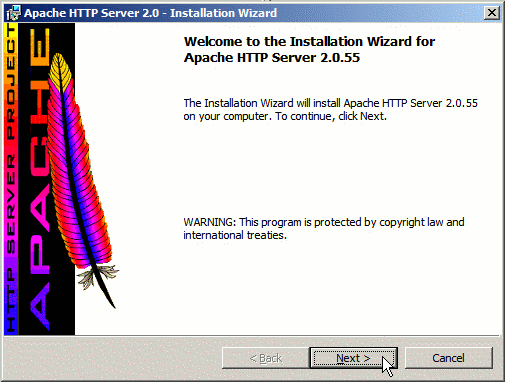
\includegraphics[scale=1,width=8cm]{ch01-01.png}
\caption{Інсталятор Apache}
\label{f1-1:image}
\end{figure}
Вам потрібно буде занести домен, в якому знаходиться сервер, ім'я сервера, e-mail адміністратора сервера. У даному випадку ці дані не важливі, їх можна залишити стандартними  (Рис.~\ref{f1-2:image}).
\begin{figure}
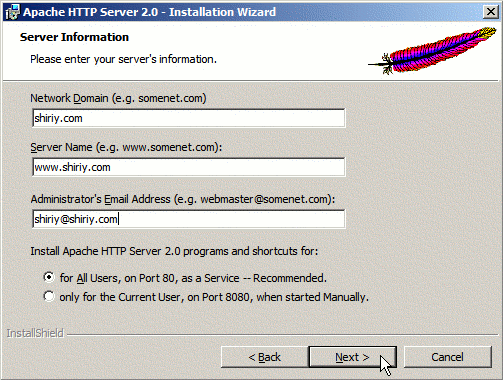
\includegraphics[scale=1,width=8cm]{ch01-02.png}
\caption{Налаштування доменних імен}
\label{f1-2:image}
\end{figure}
Також треба вибрати каталог, куди буде встановлюватися Apache, або залишити його стандартним  (Рис.~\ref{f1-3:image}). 
\begin{figure}
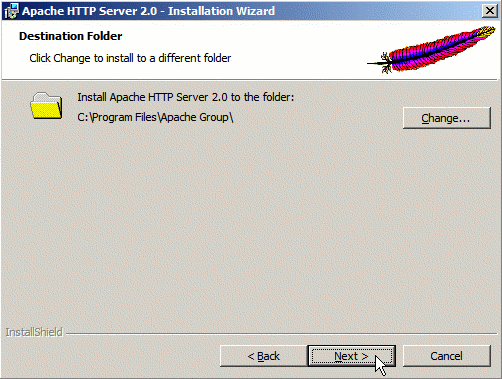
\includegraphics[scale=1,width=8cm]{ch01-03.png}
\caption{Каталог розміщення Apache}
\label{f1-3:image}
\end{figure}
Подальші зміни в конфігурації Apache можна вносити, використовуючи файл <<httpd.conf>>.

Щоб було зручно маніпулювати файлами ваших проектів створіть папку зі зрручним для вас коротким шляхом, наприклад \verb'D:\Site', в якій будуть зберігатися всі інші програми і дані сайту. Далі створіть папку \verb'D:\Site\localhost\', в якій створіть директорії WWW і CGI відповідно. WWW міститиме матеріали сайту, а CGI - скрипти CGI, якщо такі у вас будуть. В директорії \dots\verb'\Apache2\Conf\' знайдіть файл <<httpd.conf>>~--- це файл з налаштуваннями. У ньому знайдіть рядок

\begin{verbatim}
ServerRoot "C :/Program Files/Apache Group/Apache2"
\end{verbatim}

Він повинна містити шлях до самого Апач, тобто на ту папку, куди у вас Апач встановлений. Зверніть увагу, що в шляху слеш прямий і закінчується адреса без слеша.

Далі прив'язуємо Apache до конкретного порту:

\begin{verbatim}
Listen 80
\end{verbatim}

При деяких помилках сервера Apache відсилає електронні листи адміністратору, адреса поштової скриньки налаштовується у рядку

\begin{verbatim}
ServerAdmin your@email.name
\end{verbatim}

Тепер прописуємо шлях до даних сайту

\begin{verbatim}
DocumentRoot "D:/Site/localhost/WWW"
\end{verbatim}

Знайдіть блок 
\begin{verbatim}
<Directory "C:/Program Files/Apache Group/Apache2/htdocs">
\end{verbatim}

і замініть його на

\begin{verbatim}
<Directory "D:/Site">
    Options Indexes Includes
    AllowOverride All
    Order allow,deny
    Allow from all
</Directory>
\end{verbatim}

\pagebreak[3]

\section{Налаштування PHP}
\nopagebreak[4]
Встановлення PHP в середовищі Windows також не створює проблем. Завантажте встановлювач і запустіть його. 

Необхідно буде вибрати каталог для встановлення інтерпретатору, встановлену версію Apache (Рис.~\ref{f1-4:image}).
\begin{figure}
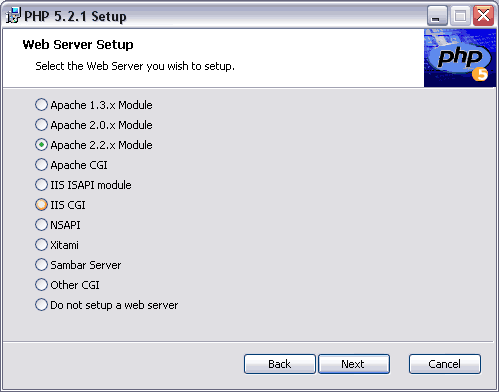
\includegraphics[scale=1,width=8cm]{ch01-04.png}
\caption{Каталог розміщення PHP}
\label{f1-4:image}
\end{figure}
Також необхідно задати місцезнаходження файлу  <<httpd.conf>> (Рис.~\ref{f1-5:image}).
\begin{figure}
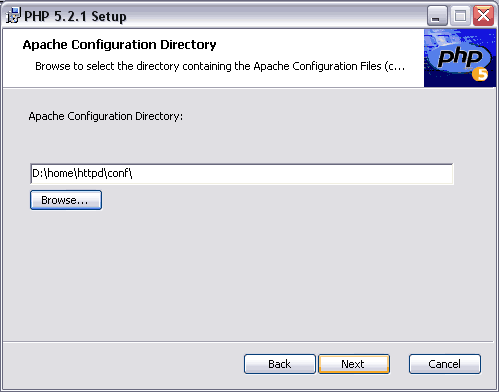
\includegraphics[scale=1,width=8cm]{ch01-05.png}
\caption{Вибір місцезнаходження файлу  <<httpd.conf>>}
\label{f1-5:image}
\end{figure}
Виберіть усі розширення PHP, що йдуть у комплекті, так ви не зіткнетесь з проблемами недостачі бібліотек під час навчання~(Рис.~\ref{f1-6:image}).

\begin{figure}
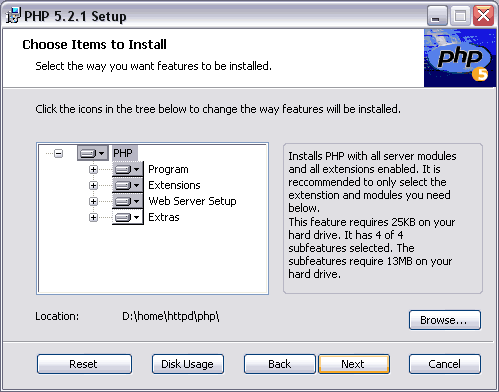
\includegraphics[scale=1,width=8cm]{ch01-06.png}
\caption{Вибір встановлюваних бібліотек}
\label{f1-6:image}
\end{figure}

У випадку проблеми прив'язки PHP до Apache його можна підключити безпосередньо у файлі <<httpd.conf>>. Для цього у файл необхідно додати такі рядки:

\begin{verbatim}
LoadModule php5_module c:/(каталог з PHP)/php5apache2_2.dll 
AddType application/x-httpd-php phtml php
PHPIniDir "c:/(каталог з PHP)/"
\end{verbatim}

Для перевірки роботи PHP та Apache створіть файл у каталозі вашого сайту <<phpinfo.php>> з такими рядками:
\pagebreak[3]
\penalty -20000
\begin{verbatim}
<?php
  echo phpinfo();
?> 
\end{verbatim}

В адресній строці браузера введіть \verb'http://localhost/phpinfo.php'. Якщо ви все виконали правильно, ви повинні побачити сторінку, зображену на Рис.~\ref{f1-7:image}:

\begin{figure}
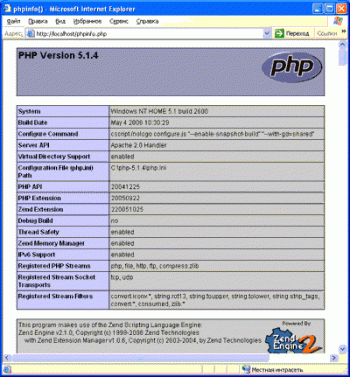
\includegraphics[scale=1,width=8cm]{ch01-07.png}
\caption{Результат роботи функції phpinfo()}
\label{f1-7:image}
\end{figure}

\pagebreak[3]

\section{Налаштування СКБД MySQL}
\nopagebreak[4]
При встановленні  СКБД MySQL вам необхідно запустити файл-інсталятор, даних за замовчуванням достатньо для встановлення повнофункціонального пакету. Після встановлення запуститься майстер налаштувань. Стандартних даних для роботи СКБД достатньо, одначе необхідно буде вказати пароль доступу адміністратора до СКБД в діалозі, зображеному на  Рис.~\ref{f1-8:image}.

\begin{figure}
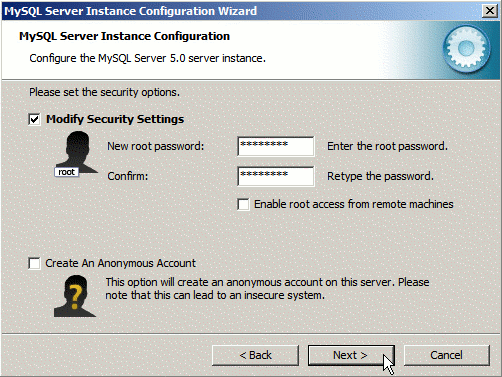
\includegraphics[scale=1,width=8cm]{ch01-08.png}
\caption{Введення пароля адміністратора СКБД}
\label{f1-8:image}
\end{figure}
Після встановлення пароля ви можете під'єднуватися до бази під логіном <<root>> та вказаним вами паролем.

\pagebreak[3]

\section{Індивідуальне завдання}
\nopagebreak[4]
\subsection*{Завдання до лабораторної роботи}
\nopagebreak[4]
\begin{enumerate}
\item Вивчити теоретичний матеріал
\item Відповісти на контрольні запитання
\item Скласти звіт
\item Захистити роботу
\end{enumerate}

\subsection*{Контрольні запитання}
\nopagebreak[4]
\begin{enumerate}
\item Що таке Internet? З яких структурних частин складається Internet?
\item Що таке IP-адреса?
\item Що таке доменне ім'я, з чого воно складається?
\item Який сервіс Internet перетворює IP-адреси в доменні імена і навпаки?
\item Яка служба займається розподіленням блоків IP-адрес?
\item Протокол HTTP. Рівень у моделі OSI, призначення.
\item Значення URI, URL, URN.
\item Мови web-програмування, які ви знаєте.
\item Веб-сервери, які ви знаєте.
\item Мережеві СКБД, які ви знаєте. 
\end{enumerate}




%\chapter{Форми HTML. Змінні, константи, масиви та функції в РНР}
\section*{Мета роботи}
Згадати основи мови розмітки веб-сторінок. Ознайомитись з базовими елементами мови РНР.
\nopagebreak[4]
\section{Формування HTML-сторінки засобами PHP}
\nopagebreak[4]
Код PHP зазвичай об'єднується з тегами XHTML. PHP є вбудовуваним мовою~--- це означає, що можна переміщатися між чистим кодом HTML і PHP, не жертвуючи можливістю читання тексту.
\index{PHP!теги відкриття/закриття}Щоб вбудувати код PHP в XHTML, PHP повинен задаватися відокремлено, за допомогою початкового та кінцевого тегів PHP. Теги PHP кажуть інтерпретатору, де починається і закінчується код PHP. Аналізатор PHP розпізнає три варіанти початкового і кінцевого тегів.

\begin{enumerate}



\item Перший варіант тегів PHP називається тегами в стилі XML і є кращим стилем. Він працює в документах розширювана мова розмітки (XML). Цей метод повинен використовуватися при з'єднанні PHP з документами XML і XHTML. Приклади в цьому підручнику застосовують цей формат тегів XML.

Стиль XML
\begin{verbatim}
<? PHP
//Блок коду PHP
>
\end{verbatim}

    
\item Скорочений стиль є найбільш простим, однак, він не рекомендується, тому що вступає в протиріччя зі стандартами документів XML та налаштуваннями в <<php.ini>>.

Скорочений стиль    
\begin{verbatim}
<?
//Блок коду PHP
>
\end{verbatim}

    
\item Цей стиль використовує найдовшу запис і схожий на стиль тегів, що застосовуються для включення кодів JavaScript. Цей стиль є кращим при використанні редактора HTML, який не розпізнає інші стилі тегів. Так як більшість нових редакторів XHTML розпізнають стиль тегів XML, то використання цього стилю не рекомендується.

Стиль сценарію
\begin{verbatim}
<script language="php">
//Блок коду PHP
</ SCRIPT>
\end{verbatim}
   
\end{enumerate}

PHP містить два основних оператора для виведення тексту в веб-браузері: \verb|echo| і  \verb|print|. Обидва оператора розміщуються між відкритим і закритим тегами блоку коду PHP і можуть перебувати в будь-якому місці в документах XHTML. Оператори  \verb|echo| і  \verb|print| використовують наступний формат:
\verb|echo|~--- використовується для виведення одного або кількох рядків.
\begin{verbatim}
echo "виведений текст";
\end{verbatim}
 \verb|print|~--- використовується для виведення рядка. В деяких випадках оператор  \verb|print| пропонує більшу функціональність, ніж оператор  \verb|echo|.
\begin{verbatim}
print "виведений текст";
\end{verbatim}
Наступні приклади демонструють використання і розміщення команд  \verb|echo| і  \verb|print| в документі XHTML.



\begin{lstlisting}[caption=Приклад вживання команд echo і print]
<!DOCTYPE html PUBLIC "-//W3C//DTD/XHTML 1.0 Transitional//EN"
  "http://www.w3.org/TR/xhtml1/DTD/xhtml11-transitional.dtd">
<html xmlns="http://www.w3.org/1999/xhtml" xml:lang="en" lang="en">
<head>
  <title> Страница Web </title>
</head>
<body>
<?php 
echo "Друк рядка оператором echo"."<br>";
print "Друк рядка оператором print";
?>
</body>
</html>
\end{lstlisting}



\pagebreak[3]
\section{Передача даних з HTML-форми PHP-сценарію}
\nopagebreak[4]
\index{HTML!передача данних}
Обробка форм є дуже важливою властивістю PHP. За допомогою форм користувачі взаємодіють зі сторінками Web, і з їхньою ж допомогою можна збирати інформацію для персоналізованих сторінок відвідувачів. У більш широкому сенсі інформаційної обробки, форми призначені для введення даних в системи обробки. Вони є первинним механізмом отримання даних, які обробляють сценарії для породження нової інформації, поновлення файлів і баз даних, а також для відповіді на запити користувачів для отримання інформації. Зовнішній вигляд типової форми дано на малюнку~\ref{f2-1:image}.

Передача даних з форм в РНР-сценарій відбувається методами  \verb|GET| або  \verb|POST| протоколу НТТР. Обидва методи однаково ефективні при використанні в формах з невеликою кількістю полів. Метод  \verb|POST| рекомендований при передачі великих обсягів тексту і файлів, обмеження за замовчуванням встановлено в 8 Мбайт і налаштовується у файлі  \verb|php.ini|.

Контейнер форми виглядає наступним чином:
\begin{verbatim}
<form name="form1" action="script.php" method="post">
</form>
\end{verbatim}
де \verb'name'~--- назва HTML-об'єкта, \verb'action' - відносний або абсолютний шлях до сценарію, якому передаються дані, \verb'method' - назва методу, яким передаються дані.

У контейнер форми поміщаються додаткові елементи управління, якими управляє користувач:

\subsection*{INPUT і його варіації}
\index{HTML!форми!input}
Елемент \verb'<input>' є найбільш вживаним тегом HTML-форм. За допомогою цього тега реалізуються основні функції форми. Він дозволяє створювати всередині форми поля введення рядка тексту, імені файлу, пароля і т.д. Також варто згадати про варіацію тега, що реалізує можливість завантаження файлів на сервер. Повний опис можливостей даного тега дано у додатку~\ref{inp-tag:app}
\subsection*{TEXTAREA}
\index{HTML!форми!textarea}
Елемент \verb'<textarea>' відповідає за передачу багаторядкового тексту. Важливо пам'ятати, що об'єм тексту, що передається обмежений параметрами методу, який використовується для передачі. Повний опис можливостей даного тега дано у додатку~\ref{tar-tag:app}
\subsection*{Списки вибору SELECT}
\index{HTML!форми!select}
Досить часто існує необхідність представити які-небудь дані у вигляді списку і передбачити можливість вибору в цьому списку. У HTML списки реалізуються за допомогою тега \verb'<select>'. Списки можуть давати можливість одиночного або множинного вибору. Повний опис можливостей даного тега дано у додатку~\ref{sel-tag:app}

\begin{figure}
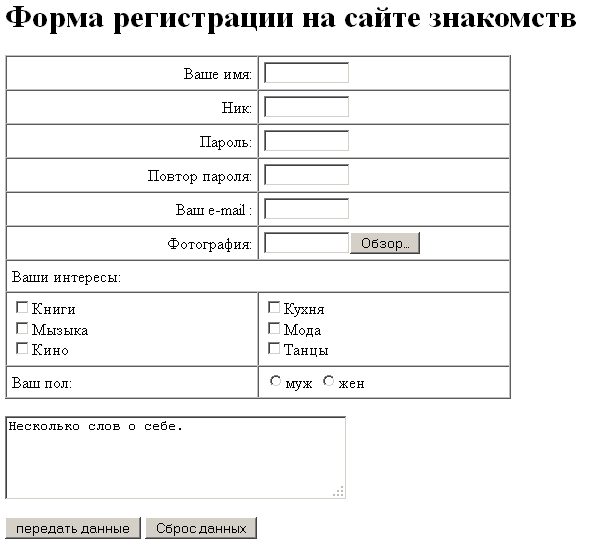
\includegraphics[scale=1,width=8cm]{ch02-01.png}
\caption{Вигляд HTML-форми}
\label{f2-1:image}
\end{figure}


\pagebreak[3]
\section{Змінні, константи та функції в РНР}
\nopagebreak[4]
\subsection*{Змінні}
\index{PHP!змінні}
\textbf{Змінні} є тимчасовим місцем зберігання, використовуваним для представлення значень в сценарії PHP. У PHP є два основні типи змінних: скалярні і масиви. Скалярні змінні містять тільки одне значення в даний момент часу, а змінні масиви - список значень. Змінні масиви обговорюються в наступному розділі. Скалярні змінні PHP містять значення типів описаних у лабораторній роботі №~\ref{datatypes}.

Імена змінних PHP всіх типів починаються зі знака <<\$>>. Імена змінних можуть містити літери, числа, і символ підкреслення (\_); вони не можуть, проте, починатися з цифри. У PHP імена змінних розрізняють регістр символів. 

\subsection*{Інтерполяція змінних}
\index{PHP!змінні!інтерполяція}
PHP підтримує також процес, званий інтерполяцією. \textbf{Інтерполяція}~--- заміна змінної в рядку її вмістом. Замість з'єднання змінних і літералів, їх можна об'єднувати всередині подвійних лапок (""). Змінні і літерали не можна об'єднати всередині одиночних лапок. При використанні подвійних лапок значення змінної виводиться разом з літералів. 
\begin{verbatim}
<?php 
$fname = "John";
$lname = "Doe";
echo "The user's name is $fname $lname";
?>
\end{verbatim}
\subsection*{Константи}
\index{PHP!константи}
\textbf{Константи}, як і змінні, є тимчасовим сховищем значень у пам'яті. На відміну від змінних значення константи ніколи не змінюється. При оголошенні константи використовується функція  \verb|define()|, яка вимагає задати ім'я константи і значення цієї константи.

Константам можна присвоювати такі типи даних.

Цілі~--- цілі числа або числа без десяткової крапки (1, 999, 325 812 841).

Числа з плаваючою точкою~--- числа, що містять десяткову крапку (1.11, 2.5, .44).

Рядки~--- текстова або числова інформація. Строкові дані завжди полягають в лапки ("Hello World", "478-477-5555").

Імена констант PHP на відміну від змінних не починаються зі знака <<\$>>. Імена констант звичайно записують у верхньому регістрі. Імена констант можуть містити літери, цифри та символ підкреслення (\_); вони не можуть, проте, починатися з цифри. Оголошення констант показано нижче.
\begin{verbatim}
define ("STRING_CONSTANT", "This is my string."); 
define ("NUMERIC_CONSTANT", 5); 
\end{verbatim}
Вивід констант подібний до виводу змінних.
\subsection*{Функції}
\index{PHP!функції}
\textbf{Функцією} називається фрагмент програмного коду, що володіє унікальним ім'ям і призначений для вирішення певного завдання. 

Функції використовуються для розбиття великих блоків коду на менші, більш керовані одиниці. Код, що міститься всередині функції, виконує певне завдання і повертає значення. PHP містить два типи функцій~--- визначені користувачем (або створені програмістом) і внутрішні (вбудовані функції), які є частиною визначення мови PHP.

Виклик вбудованої функції відбувається за допомогою її імені. Наприклад, функція, що виводить інформацію про РНР та Apache:
\begin{verbatim}
<?php
phpinfo();
?>
\end{verbatim}
У даному випадку функція викликається без параметрів. Наступна функція використовує ряд аргументів і повертає значення (у даному випадку дескриптор відкритого файлу:
\begin{verbatim}
<?php
f=fopen("d:\www\index.php","w+");
?>
\end{verbatim}
\pagebreak[3]
\section{Робота з масивами в РНР}
\nopagebreak[4]
\index{PHP!змінні!масиви}
Змінну масиву можна використовувати для зберігання множини або послідовності значень. Система PHP підтримує масиви з числовими індексами і асоціативні масиви. \textbf{Масив} в PHP є фактично впорядкованим відображенням. Відображення є типом, який відображає значення в ключі. Змінні масивів складаються з двох частин~--- індексу та елемента. Індекс масиву, іноді званий ключем масиву, є значенням, застосовуваним для ідентифікації або доступу до елементів масиву. Індекс масиву поміщається в квадратні дужки. Більшість масивів використовують числові індекси, які зазвичай починаються з 0 або 1. У PHP асоціативні масиви можуть використовувати рядкові індекси. Обидва типи масивів створюються за допомогою конструкції  \verb|array()|
\subsection*{Масиви з числовими індексами}
\begin{verbatim}
$my_array = array('red', 'green', 'blue'); 
\end{verbatim}
Цей код створює масив з числовим індексом з ім'ям \verb'$my_array'. Масиву присвоюється три елементи~---  \verb|red|,  \verb|green| і  \verb|blue|. Кожен елемент ідентифікується числовим індексом.
\begin{verbatim}
$my_array [0] = 'red' // індекс 0 відповідає елементу red 
$my_array [1] = 'green' // індекс 1 відповідає елементу green 
$my_array [2] = 'blue' // індекс 2 відповідає елементу blue 
\end{verbatim}
Щоб отримати доступ до вмісту масиву, використовується ім'я масиву та індекс. 
\subsection*{Асоціативні масиви}
Асоціативні масиви дозволяють використовувати більш корисні значення індексу. Для масивів з числовими індексами значення індексу створюються автоматично, починаючи з 0. Асоціативні масиви допускають застосування числових і строкових значень індексу.
\begin{verbatim}
$members = array('FName' => 'John', 'LName' => 'Smith', 'Age' => 50) 
\end{verbatim}
У цьому прикладі члени масиву містять три елементи, однак використовуються рядкові індекси~---  \verb|FName|,  \verb|LName| і  \verb|Age|.
\begin{verbatim}
$members ['FName'] = 'John' // індекс FName відповідає елементу John
$members ['LName'] = 'Smith' // індекс LName відповідає елементу Smith
$members ['Age'] = '50 '// індекс Age відповідає елементу 50 
\end{verbatim}
Для доступу до вмісту масиву використовується ім'я масиву та індекс.
\pagebreak[3]
\section{Функції, визначені користувачем}
\nopagebreak[4]
\index{PHP!функції!користувацькі функції}
\textbf{Визначені користувачем функції} створюються за допомогою ключового слова \verb'function'. Вони особливо корисні у великих програмах PHP, так як можуть містити блоки коду, які можуть використовуватися в програмі, що дозволяє уникнути повторного переписування коду. Далі представлений приклад простої визначеної користувачем функції PHP:
\begin{verbatim}
function AddNumbers ($num1, $num2)
{
echo "Це приклад функції PHP. 
Вона обчислює суму двох чисел і повертає 
результат програмі, що її викликала";
return $num1 + $num2;
} 
\end{verbatim}


Визначені користувачем функції можуть викликатися в будь-якому місці програми на PHP. У PHP функція виконується при використанні в коді її імені. Після виклику функція отримує всі передані їй значення у формі параметрів, виконує певні завдання і повертає значення програмі. 

\pagebreak[3]
\section{Змінні всередині функції}
\nopagebreak[4]
\index{PHP!змінні!локальні змінні}
\index{PHP!змінні!глобальні змінні}
\textbf{Глобальні змінні}~--- це змінні, які доступні всій програмі, включаючи підпрограми (користувальницькі функції).

\textbf{Локальні змінні}~--- змінні, визначені всередині підпрограми (користувацької функції). Вони доступні тільки всередині функції, в якій вони визначені.

Для PHP всі оголошені і використовувані у функції змінні за замовчуванням локальні для функції. Тобто, за умовчанням немає можливості змінити значення глобальної змінної в тілі функції. 

існує спеціальна інструкція \verb'global', що дозволяє функції користувача працювати з глобальними змінними. Розглянемо даний принцип на конкретному прикладі:

\begin{verbatim}
<?php
$a = 1 ;
$b = 2 ;

function sum()
{
global $a, $b;
$b = $a + $b;
}
?> 
\end{verbatim}

\pagebreak[3]
\section{Змінні-функції}
\nopagebreak[4]
\index{PHP!функції!змінні-функції}
PHP підтримує концепцію \textbf{змінних-функцій}. Це означає, що якщо до імені змінної приєднані круглі дужки, PHP шукає функцію з тим же ім'ям, що і результат обчислення змінної, і намагається її виконати. Цю можливість можна використовувати для реалізації зворотних викликів, таблиць функцій і безлічі інших речей.

Приклад використання змінної-функції наведено в додатку~\ref{var-func:app}

\pagebreak[3]
\section{Індивідуальне завдання}

\nopagebreak[4]
\subsection*{Завдання до лабораторної роботи}
\nopagebreak[4]
\begin{enumerate}
\item Вивчити теоретичний матеріал
\item Відповісти на контрольні запитання
\item Скласти алгоритм (блок-схему) програми
\item Виконати практичне завдання
\item Скласти звіт
\item Захистити роботу
\end{enumerate}

\subsection*{Контрольні запитання}
\nopagebreak[4]
\begin{enumerate}
\item Що таке змінні, константи та функції?
\item Що таке інтерполяція змінних?
\item Що таке масиви?
\item Як отримати доступ до індексного масиву? 
\item До ассоціативного?
\item Як створити користувацьку функцію?
\item Що таке локальні змінні?
\item Що таке глобальні змінні? Як ними користуватись у тілі функції?
\item Що таке змінні-функції?
\item Яким чином здійснюється виклик функції-змінної?
\end{enumerate}

\subsection*{Практичні завдання}
\nopagebreak[4]


\begin{enumerate}
\item[]Написати HTML-сторінку з формою, що складається з:
\item однорядкового поля вводу, поля вводу пароля та кнопки відправлення форми.
\item однорядкового поля вводу, прихованого текстового поля та кнопки відправлення форми.
\item однорядкового поля вводу, багаторядкового поля вводу та кнопки відправлення форми.
\item багаторядкового поля вводу, списку з одиночним вибором з п'яти елементів та кнопки відправлення форми.
\item прихованого текстового поля, списку з одиночним вибором з п'яти елементів та кнопки відправлення форми.
\item багаторядкового поля вводу, списку з множинним вибором з п'яти елементів та кнопки відправлення форми.
\item списку з одиночним вибором з п'яти елементів, поля вводу пароля та кнопки відправлення форми.
\item списку з множинним вибором з п'яти елементів, багаторядкового поля вводу та кнопки відправлення форми.
\item[]Отримати дані форми і вивести іх за допомогою функції в окремому сценарії.
\item створити асоціативний масив з днями тижня та вивести його на сторінку
\item створити індексний массив з назвами місяців і вивести його на екран
\item[]Написати HTML-сторінку з формою, що складається з однорядкового поля вводу та кнопки відправлення. Записати в поле число та обробити наступним чином:
\item створити константу та помножити на отримане з форми число 
\item створити змінну, занести в неї результат з форми, помножити змінну саму на себе
\item створити константу та обчислити вираз $x*const+2*x$
\item створити константу та обчислити вираз $\frac{x}{const}+x^2$
\item створити змінну та константу, в змінну занести константу і додати до числа з форми.
\item[]Результат вивести на сторінку 
\item[]Створити форму з трьома однорядковими полями і кнопкою відправлення форми
\item отримані з форми дані занести в асоціативний масив
\item отримані дані занести в індексний масив
\item[]зміст масиву роздрукувати функцією \verb'print_r()'; 
\item створити функцію, що друкує свій параметр
\item створити функцію, що перемножує два свої параметри і повертає результат. Результат роздрукувати
\item створити функцію, що перемножує свої параметри і друкує результат
\item створити функцію, що змінює глобальну змінну
\item створити функцію, що перемножує глобальну змінну і вхідний параметр, рузультат друкує
\item створити функцію, що домножує глобальну змінну на вхідний параметр і повертає результат
\item створити функцію, що формує індексний масив з двох локальних змінних і друкує його функцією \verb'print_r()';
\item створити функцію, що формує асоціативний масив з параметрів і друкує його функцією \verb'print_r()';

\end{enumerate}




%\chapter{Взаємодія PHP та web-сервера. Синтаксис PHP}
\nopagebreak[4]
\section*{Мета роботи}
Ознайомитись зі змінними оточення веб-серверу та суперглобальними масивами РНР. Ознайомитись з конструкціями розгалуження, циклів, включення файлів.
\section{Змінні оточення web-сервера Apache, суперглобальні масиви PHP}
\nopagebreak[4]

\subsection*{Змінні оточення web-сервера Apache}
\index{Web-сервери!Apache!змінні оточення}
\textbf{Змінні оточення}~--- дуже важливий механізм взаємодії веб-сервера з предобработчікамі запитів. При отриманні HTTP-запиту веб-сервер формує змінні оточення, заносячи в них різну інформацію: IP-адреса клієнта, запитуваний документ, параметри запиту і т.п. При передачі управління якомусь предобработчіку останній має доступ до змінних оточення веб-сервера, отже, йому доступна вище перерахована інформація.

Безпосередньо перед запуском сценарію сервер передає йому якісь змінні оточення з інформацією. Змінні оточення в мові PHP можна використовувати як звичайнісінькі змінні. Змінні оточення діляться на чотири великі групи:
\begin{enumerate}
\item Формовані сервером змінні;
\item Спеціальні змінні сервера Apache;
\item Змінні HTTP-полів запиту;
\item Змінні SSL-з'єднання (захищеного з'єднання).
\end{enumerate}

\subsection*{Суперглобальні масиви PHP}
\index{PHP!змінні!суперглобальні масиви}
\textbf{Суперглобальними масивами} (superglobal arrays) в PHP називаються зумовлені масиви, які видно в будь-якому місці вихідного коду без використання ключового слова \verb'global'.


Доступ до змінних оточення здійснюється через суперглобальний масив \verb'$_SERVER' у вигляді \verb|$_SERVER['змінна_CGI']|; Наприклад код
\begin{verbatim}
print $_SERVER['SERVER_SOFTWARE'];
\end{verbatim}
роздрукує в браузері строку виду:
\begin{verbatim}
Apache/2.2.4 (Win32) mod_ssl/2.2.4 OpenSSL/0.9.8k PHP/5.3.3
\end{verbatim}


Повний перелік змінних оточення web-сервера Apache та суперглабальних масивів PHP дивіться у додатках~\ref{var-apa:app} та~\ref{sup-glob:app}.


\pagebreak[3]



\section{Оператори PHP}
\nopagebreak[4]
\index{PHP!оператори}
Синтаксис PHP дуже нагадує синтаксис мови C і багато в чому запозичений з таких мов як Java і Perl. Інструкції поділяються також як і в C або Perl~--- кожен вираз закінчується крапкою з комою. Закриваючий тег <<?> >> також має на увазі кінець інструкції.

Коментарі застосовуються в PHP для запису власних зауважень під час процесу розробки коду. Такі коментарі можуть визначати призначення сегмента коду або їх можна використовувати для виключення блоків коду під час тестування і налагодження сценаріїв.

Синтаксичний аналізатор PHP ігнорує коментарі. Коментарі в PHP можна визначити одним з наступних способів:
\begin{enumerate}

\item \verb|//|~--- Простий коментар PHP;
\item \verb|#|~--- Альтернативний простий коментар PHP;
\item \verb|/* ... */|~--- Багаторядкові блоки коментарів.

\end{enumerate}
\penalty -10000
Імена змінних позначаються знаком \$.

\begin{verbatim}
<?php
$message = "Привет, я - скрипт PHP!";
echo $message;
?>
\end{verbatim}
\index{PHP!змінні!типи даних}
PHP підтримує вісім простих типів даних \label{datatypes}:
\begin{enumerate}
\item Чотири скалярних типи:
		\begin{itemize}
		\item Boolean (двійкові дані)
		\item Integer (цілі числа)
		\item Float (числа з плаваючою точкою або 'double')
		\item String (рядки)
		\end{itemize}
\item Два змішаних типи:
		\begin{itemize}
		\item Array (масиви)
		\item Object (об'єкти)
		\end{itemize}
\item Два спеціальних типи:
		\begin{itemize}
		\item resource (ресурси)
		\item NULL (<<порожні>>)
		\end{itemize}
\item Існують також кілька псевдотіпов:
		\begin{itemize}
		\item Mixed (змішані)
		\item Number (числа)
		\item Callback (зворотний визов)		
		\end{itemize}
\end{enumerate}

Основними конструкціями мови PHP є:
\index{PHP!конструкції}
\begin{enumerate}
\item Умовні оператори (\verb|if, else|);
\item Цикли (\verb|while, do-while, for, foreach, break, continue|);
\item Конструкції вибору (\verb|switch|);
\item Конструкції оголошення (\verb|declare|);
\item Конструкції повернення значень (\verb|return|);
\item Конструкції включень (\verb|require, include|).
\end{enumerate}


Для здійснення операцій зі змінними існують різні групи операторів. Оператором називається дещо, що складається з одного або більше значень (виразів), яке можна обчислити як нове значення (таким чином, вся конструкція може розглядатися як вираз).

\textbf{Оператори бувають трьох видів.}
\begin{enumerate}
\item Унарні оператори, які працюють тільки з одним аргументом, наприклад, <<!>> (оператор заперечення) або <<++>> (інкрімент).
\item Бінарні оператори: до них належать більшість підтримуваних в PHP операторів
\item тернарних оператор <<\dots?\dots:\dots>>. Він використовується для умовного вибору між двома операторами, в залежності від результату обчислення третього оператора.
\end{enumerate}
\subsection*{Пріоритет виконання операторів}
\index{PHP!оператори!пріоритети}
Пріоритет операторів визначає, в якому порядку будуть обчислюватися два і більше вирази. Наприклад, вираз $1 + 5 * 3$ обчислюється як 16, а не 18, оскільки операція множення <<*>> має більш високий пріоритет, ніж операція додавання <<+>>. У разі, якщо оператори мають однаковий пріоритет, вони будуть виконуватися зліва направо. Круглі дужки можуть використовуватися для примусового вказівки необхідного порядку виконання операторів. Наприклад, вираз $(1 + 5) * 3$ обчислюється як 18.

В таблиці~\ref{pr-op:table} додатку надано пріоритети виконання операторів PHP.

Ліва асоціативність вказує на те, що вираз обчислюється зліва направо, права асоціативність відповідно має увазі протилежний порядок.
\pagebreak[3]
\section{Конструкції вибору}
\index{PHP!конструкції!розгалуження}
\nopagebreak[4]
До конструкцій вибору відносять: умовний оператор (\verb'if...else') і перемикач (\verb'switch'). 
\subsection*{if \dots else}
Синтаксис умовного оператора:
\begin{verbatim}
if (condition) statement1 else statement2
\end{verbatim}


Умова \verb'condition' може бути будь-яким виразом. Якщо \verb'condition' істинне, то виконується оператор \verb'statement1' . В іншому випадку виконується оператор \verb'statement' 2. Допустима скорочена форма запису умовного оператора, в якій відсутні \verb'else' і оператор \verb'statement2'.

У свою чергу, оператори \verb'statement1' і \verb'statement2' можуть бути умовними, що дозволяє організовувати послідовність перевірок будь-якої глибини вкладеності. І в цих послідовностях кожен умовний оператор може бути як повним, так і скороченим. У зв'язку з цим можливі помилки неоднозначного зіставлення \verb'if' і \verb'else'.

Зауважимо, що перевірка додаткових умов можлива за допомогою оператора \verb|elseif|. Оператор \verb|if| може включати скільки завгодно блоків \verb'elseif', але else в кожному if може бути тільки один. Як правило, в конструкціях \verb'if ... elseif ... else' оператор else визначає, що потрібно робити, якщо ніякі інші умови не є true. 

РНР надає також можливість альтернативного синтаксису умовного оператора~--- без фігурних дужок, а із застосуванням оператора \verb'endif', при цьому оператори будуть розміщені всередині блока.

\subsection*{Перемикач <<switch>>}

Перемикач \verb'switch' є найбільш зручним засобом для організації множинного розгалуження. Синтаксис перемикача такий:
\penalty -10000
\begin{verbatim}
switch (expression) 
{
case value1: statements; break;
case value2: statements; break;
default:
statements;
}
\end{verbatim}

Керуюча структура \verb'switch' передає керування тому з помічених \verb'case' операторів, для якого значення константного виразу збігається зі значенням \verb'expression'. Якщо значення \verb'expression' не збігається ні з одним з константних виразів, то виконується перехід до оператора, поміченого міткою \verb'default'. У кожному перемикачі може бути не більше однієї мітки \verb'default', однак вона може бути відсутньою взагалі.


\pagebreak[3]

\section{Конструкції циклів}
\nopagebreak[4]

\index{PHP!конструкції!цикли}

На другому місці за частотою використання, після конструкцій умов (умовних операторів), знаходяться цикли.

Цикли дозволяють повторювати певну (і навіть невизначений~--- коли робота циклу залежить від умови) кількість разів різні послідовності операторів. Дані оператори називаються тілом циклу. Прохід циклу називається ітерацією.

PHP підтримує чотири види циклів:
\begin{itemize}
\item    Цикл з передумовою (while)
\item    Цикл з постусловіем (do-while)
\item    Цикл з лічильником (for)
\item    Спеціальний цикл перебору масивів (foreach)
\end{itemize}

Цикли зручно також використовувати при форматуванні HTML-сторінки. Наприклад при створенні великих списків або таблиць.

\begin{lstlisting}[caption=Формування HTML-сторінки за допомогою циклів]
<!DOCTYPE html PUBLIC "-//W3C//DTD/XHTML 1.0 Transitional//EN"
  "http://www.w3.org/TR/xhtml1/DTD/xhtml11-transitional.dtd">
<html xmlns="http://www.w3.org/1999/xhtml" xml:lang="en" lang="en">
<head>
  <title> Страница Web </title>
</head>
<body>
<table>
<?php
for (int $i=1; $i<=10; $i++) 
echo "<tr><td> Рядок № </td><td>$i</td></tr>\n";
?>
</table>
</body>
</html>
\end{lstlisting}




Сценарій для тієї самої сторінки без використання циклів зайняв б у два рази більше дискового простору.

При використанні циклів є можливість використання операторів \verb'break' і \verb'continue'. Перший з них перериває роботу всього циклу, а другий~--- тільки поточної ітерації.


\subsection*{Цикл з передумовою while}
\index{PHP!конструкції!while}
Цикл з передумовою while працює за такими принципами:

\begin{enumerate}
\item    Обчислюється значення логічного виразу.
\item    Якщо значення істинно, виконується тіло циклу, в іншому випадку~--- переходимо на наступний за циклом оператор.
\end{enumerate}


Синтаксис циклу з передумовою:
\begin{verbatim}
while (логічний_вираз) інструкція;
\end{verbatim}

В даному випадку тілом циклу є інструкція. Зазвичай тіло циклу складається з великої кількості операторів. Наведемо приклад циклу з передумовою while:
\begin{verbatim}
<? Php
$х = 0;
while ($x++<10) echo $x;
// Виводить 12345678910
?>
\end{verbatim}
Зверніть увагу на послідовність виконання операцій умови \$x++<10. Спочатку перевіряється умова, а тільки потім збільшується значення змінної. Якщо ми поставимо операцію інкремента перед змінної (++\$x<10), то спочатку буде виконано збільшення змінної, а тільки потім~--- порівняння. У результаті ми отримаємо рядок <<123456789>>. 


Подібно конструкції умовного оператора \verb'if', можна групувати оператори всередині тіла циклу while, використовуючи наступний альтернативний синтаксис:
\begin{verbatim}
while (логічний_вираз):
інструкція;
...
endwhile;
\end{verbatim}

\subsection*{Цикл з постумовою do while}
\index{PHP!конструкції!do while}
На відміну від циклу \verb'while', цей цикл перевіряє значення виразу не до, а після кожного проходу (ітерації). Таким чином, тіло циклу виконується хоча б один раз. Синтаксис циклу з постумовою такий:
\begin{verbatim}
do
{
тело_цікла;
}
while (логічний_вираз);
\end{verbatim}
Після чергової ітерації перевіряється, чи істинний \verb'логічний_вираз', і, якщо це так, управління передається знову на початок циклу, в іншому випадку цикл обривається.

\subsection*{Цикл з лічильником <<for>> (регулярний цикл)}
\index{PHP!конструкції!for}
Цикл з лічильником використовується для виконання тіла циклу певне число разів. 

Синтаксис циклу \verb'for' такий:
\begin{verbatim}
for (ініціалізуючі_команди; умова_роботи; 
	команди_після_ітерації) {тіло_цикла;}
\end{verbatim}
Цикл for починає свою роботу з виконання \verb'ініціалізуючіх_команди'. Дані команди виконуються тільки один раз. Після цього перевіряється \verb'умова_роботи', якщо воно істинно (true), то виконується \verb'тіло_цикла'. Після того, як буде виконаний останній оператор тіла, виконуються \verb'команди_після_ітерації'.



Для циклу for є і альтернативний синтаксис:
\begin{verbatim}
for (ініціалізуючі_команди; умова_роботи; 
команди_після_ітерації):
оператори;
endfor;
\end{verbatim}

\subsection*{Цикл перебору масивів <<foreach>>}
\index{PHP!конструкції!foreach}
В PHP4 з'явився ще один спеціальний тип циклу~--- \verb'foreach'. Даний цикл призначений спеціально для перебору масивів.

Синтаксис циклу \verb'foreach' виглядає наступним чином:
\begin{verbatim}
foreach (масив as $ключ => $значення)
команди;
\end{verbatim}
Тут команди циклічно виконуються для кожного елемента масиву, при цьому чергова пара <<ключ => значення>> виявляється в змінних \verb'$ключ' і \verb'$значення'. 

У циклу foreach є й інша форма запису, яку слід застосовувати, коли нас не цікавить значення ключа чергового елемента. Виглядає вона так:
\begin{verbatim}
foreach (масив as $значення)
команди;
\end{verbatim}
У цьому випадку доступно лише значення чергового елементу масиву, але не його ключ. Це може бути корисно, наприклад, для роботи з масивами-списками:



Увага: Цикл \verb'foreach' оперує не вихідним масивом, а його копією. Це означає, що будь-які зміни, які вносяться в масив, не можуть бути <<видимі>> з тіла циклу. Що дозволяє, наприклад, в якості масиву використовувати не тільки змінну, але і результат роботи якої-небудь функції, що повертає масив (у цьому випадку функція буде викликана всього один раз~--- до початку циклу, а потім робота буде проводитися з копією повернутого значення).

\subsection*{Конструкція <<break>>}
\index{PHP!конструкції!break}
Дуже часто для того, щоб спростити логіку якого-небудь складного циклу, зручно мати можливість його перервати в ході чергової ітерації (наприклад, при виконанні якого-небудь особливого умови). Для цього і існує конструкція break, яка здійснює негайний вихід з циклу. Вона може задаватися з одним необов'язковим параметром~--- числом, яке вказує, з якого вкладеного циклу має бути здійснений вихід. За замовчуванням використовується 1, тобто вихід з поточного циклу, але іноді застосовуються й інші значення. Синтаксис конструкції \verb'break':
\begin{verbatim}
break; // За замовчуванням
break (номер_цикла); // Для вкладених циклів 
(вказується номер циклу, що переривається)
\end{verbatim}

\subsection*{Конструкція <<continue>>}
\index{PHP!конструкції!continue}
Конструкція \verb'continue' так само, як і \verb'break', працює тільки <<в парі>> з циклічними конструкціями. Вона негайно завершує поточну ітерацію циклу та переходить до нової (звичайно, якщо виконується умова циклу для циклу з передумовою). Точно так само, як і для \verb'break', для continue можна вказати рівень вкладеності циклу, який буде продовжений з повернення управління.


\pagebreak[3]

\section{Конструкції включення}
\nopagebreak[4]
Конструкції включень дозволяють збирати PHP програму (скрипт) з декількох окремих файлів.

У PHP існують дві основні конструкції включень: \verb'require' і \verb'include'.
\subsection*{Конструкція включень <<require>>}
\index{PHP!конструкції!require}
Конструкція \verb'require' дозволяє включати файли в сценарій PHP до виконання сценарію PHP. Загальний синтаксис \verb'require' такий:
\begin{verbatim}
require им'я_файлу;
або
require (им'я_файлу);
\end{verbatim}
При запуску (саме при запуску, а не при виконанні!) Програми інтерпретатор просто замінить інструкцію на вміст файлу \verb|им'я_файлу| (цей файл може також містити сценарій на PHP, обрамлений, як зазвичай, тегами << <? >> та << ?> >>'). Причому зробить він це безпосередньо перед запуском програми (на відміну від include , який розглядається нижче). Це буває досить зручно для включення в висновок сценарію різних шаблонних сторінок HTML-кодом. 
\subsection*{Конструкція <<include>>}
\index{PHP!конструкції!include}
Конструкція \verb'include' також призначена для включення файлів в код сценарію PHP.

На відміну від конструкції \verb'require' конструкція \verb'include' дозволяє включати файли в код PHP скрипта під час виконання сценарію. Синтаксис конструкції \verb'include' виглядає наступним чином:
\penalty -10000
\begin{verbatim}
include им'я_файлу;
або
include (им'я_файлу);
\end{verbatim}

Принципова різниця між цими двома операторами в тому, що \verb'include' дозволяє включати файли <<на літу>>, і робити це декілька разів, наприклад у циклах.
\subsection*{Конструкції одноразового включення <<require\_once>> і <<include\_once>>}
\index{PHP!конструкції!require\_once} \index{PHP!конструкції!include\_once}
У великих PHP сценаріях інструкції \verb'include' і \verb'require' застосовуються дуже часто. Тому стає досить складно контролювати, як би випадково не включити один і той же файл декілька разів, що найчастіше призводить до помилки, яку складно виявити.

У PHP передбачено вирішення даної проблеми. Використовуючи конструкції одноразового включення \verb'require_once' і \verb'include_once', можна бути впевненим, що один файл не буде включено двічі. Працюють конструкції одноразового включення \verb'require_once' і \verb'include_once' так само, як і \verb'require' і \verb'include' відповідно. Різниця в їх роботі лише в тому, що перед включенням файлу інтерпрететор перевіряє, чи включений вказаний файл раніше чи ні. Якщо так, то файл не буде включено знову. 

\subsection*{Включення віддалених файлів}

Конструкції однократних включень \verb'require_once' і \verb'include_ince' також дозволяють включати віддалені файли, якщо така можливість включена в конфігураційному файлі PHP.

Якщо \verb'URL fopen' увімкнено в PHP (як у конфігурації за замовчуванням), ви можете специфікувати файл, що підключається з використанням URL (через HTTP), замість локального шляху. 

Для того, щоб віддалене включення файлів було доступно, необхідно в конфігураційному файлі (php.ini) встановити \verb'allow_url_fopen = 1'.


\pagebreak[3]

\section{Конструкція <<or exit()>> (<<or die()>>)}
Конструкція складається з логічного оператора \verb'or' та функції \verb'exit()' або її псевдоніма \verb'die()'. Функція \verb'exit(статус)' друкує на екрані статус, котрий може бути цілочисельною або рядковою константою. Конструкцію зручно використовувати під час налагодження сценаріїв у комбінації з функціями, які можуть повертати логічне \verb'FALSE'. Наприклад зупинку сценарію при невдалому відкритті файлу можна отримати таким чином:
\begin{verbatim}
$file = fopen("file.txt","w+") or die("Помилка відкриття файлу");
\end{verbatim} 



\pagebreak[3]

\section{Індивідуальне завдання}

\nopagebreak[4]
\subsection*{Завдання до лабораторної роботи}
\nopagebreak[4]
\begin{enumerate}
\item Вивчити теоретичний матеріал
\item Відповісти на контрольні запитання
\item Скласти алгоритм (блок-схему) програми
\item Виконати практичне завдання
\item Скласти звіт
\item Захистити роботу
\end{enumerate}

\subsection*{Контрольні запитання}
\nopagebreak[4]
\begin{enumerate}
\item Які оператори виводу тексту ви знаєте?
\item Які групи змінних оточення ви знаєте?
\item Що таке суперглобальні масиви, як ними користуватись?
\item Яким чином можна задати коментар?
\item Які типи операторів ви знаєте?
\item Які конструкції вибору ви знаєте?
\item Які конструкції циклів ви знаєте?
\item У якому випадку цикл виконується хоча-б один раз?
\item Якими чином можна включити інший текстовий файл у сценарій?
\item Яка особливість операторів <<include\_once>> та <<require\_once>>? 
\end{enumerate}

\subsection*{Практичні завдання}
\nopagebreak[4]


\begin{enumerate}
 
\item[]Створити окремий РНР-файл, підключити його у головну сторінку. Файл повинен:
\item У регулярному циклі виводити числа від 1 до 20
\item У циклі з передумовою виводити числа від 20 до 50
\item У циклі з постумовою вивести числа від -50 до -10
\item Використовуючи регулярний цикл вивести елементи арифметичної прогресії з 20 елементів починаючи з 1 та доданком 2
\item Використовуючи з передумовою вивести елементи геометричної прогресії з 20 елементів починаючи з 1 та доданком 2
\item Розрахувати факторіал 10 за допомогою регулярного циклу
\item Вивести латинський алфавіт, використовуючи регулярний цикл
\item Вивести латинський алфавіт, використовуючи цикл з передумовою
\item Вивести Цифри від 20 до 0 у зворотньому порядку, використовуючи цикл з постумовою.
\item[]Написати HTML-сторінку з формою, що складається з однорядкового поля вводу та кнопки відправлення форми. В поле вводу ввести число та обчислити вираз: 
\item якщо $x>0$ то $5*x^2 + 2*x - 10$, інакше $5*x^2 + 2*x + 10$
\item якщо $0<x\le 10$ то $10*x^3 - 2*x - 10$, інакше $x^2 + 20*x$
\item якщо $0<x\le 20$ то $\frac{x}{x+1} + 2*x - 10$, інакше $\frac{x+1}{x} + 10$
\item якщо $-10<x\le 0$ то $5*x^2 + 2*x - 10$, $x> 0$ $5*x^2 + 2*x + 10$, інакше $\frac{x+1}{x} + 10$
\item якщо $x\le 10$ то $x^3 + 2*x^2$, інакше $2*x + 10$
\item якщо $x>10$ то $5*x^2 + \frac{x}{2}$, інакше $\frac{x+10}{x+1}$
\item[]Написати HTML-сторінку з формою, що складається з однорядкового поля вводу та кнопки відправлення форми. В поле вводу ввести число та використовуючи конструкцію <<switch-case>>: 
\item за номером дня тижня вивести його назву.
\item за номером місяця року вивести його назву.
\item від 0 до 10 вивести назви цифр
\item відповідно номера вивести букву латинського алфавіту
\item[]Опрацювати змінні оточення 
\item вивести шлях до каталогу з веб-документами
\item вивести підпис веб-сервера
\item вивести інформацію про браузер користувача
\item вивести адресу електронної пошти адміністратора
\item за допомогою конструкції перебору масивів вивести зміст \$\_SERVER
\item за допомогою конструкції перебору масивів вивести зміст \$\_ENV

\end{enumerate}

%\chapter{Робота з рядками. Регулярні вирази}
\section*{Мета роботи}
Ознайомитись із засобами роботи з рядковими змінними та константами. Ознайомитись із застосуванням регулярних виразів у мові РНР та SQL-запитах.
\nopagebreak[4]
\section{Рядки. Функції роботи з рядками}
\nopagebreak[4]
\index{PHP!змінні!рядки}
\textbf{Рядки є послідовностями символів}. У PHP символ відповідає байту, тобто існує точно 256 можливих різних символів. Рядки можуть бути дуже великими. У PHP не існує практичного обмеження на розмір рядків, тому взагалі немає причин турбуватися про їх довжині. Строкові значення можуть використовуватися буквально або присвоюватися змінним.

У PHP рядковий літерал можна задати трьома способами.
\begin{itemize}
\item рядки в одиночних лапках
\item рядки в подвійних лапках
\item рядки в синтаксисі heredoc 
\end{itemize}

\subsection*{Рядки в одиночних лапках}
Одиночні лапки надають найпростіший метод для роботи з рядками. При використанні цього методу рядки укладаються в одиночні лапки <<''>>. Якщо одиночні лапки потрібні як частина рядка, вони повинні бути екрановані символом зворотної косої межі <<\\>>. Хоча одиночні лапки надають простий спосіб роботи з рядками, одиночні лапки не підтримують застосування інтерполяції.
\subsection*{Рядки в подвійних лапках}
Рядки PHP можна виводити також за допомогою подвійних лапок <<"">>. Якщо рядки PHP поміщаються в подвійні лапки, то можна застосовувати інтерполяцію. Для рядків у подвійних лапках PHP підтримує також більшість екранованих символів. Ці символи представлені в таблиці~\ref{doub-lap:table} нижче.

\begin{center}
\begin{longtable}[t]{|l|p{20em}|}
\caption{Екрановані символи у подвійних лапках} \label{doub-lap:table}\\
\hline
Символ & Опис \\
\hline
\verb'\N' & перенесення рядка \\
\verb'\R' & повернення каретки \\
\verb'\T' & горизонтальна табуляція \\
\verb'\\' & зворотна коса риска \\
\verb'\$' & знак долара \\
\verb'\"' & подвійні лапки \\
\hline
\end{longtable}
\end{center}

\subsection*{Рядки в синтаксисі heredoc}
\textbf{Heredoc}-синтаксис~--- спосіб визначення строкових змінних у вихідному коді програм.

При визначенні строкових змінних їх вміст, зазвичай, полягає в одинарні або подвійні лапки, у зв'язку з чим символи лапок, які повинні бути частиною даних, доводиться екранувати за допомогою escape-послідовностей. Heredoc-синтаксис дозволяє визначити рядок, не укладаючи її в лапки, у зв'язку з чим необхідність екранування цих символів відпадає.

Приклад використання такого синтаксису наведено нижче:
\begin{verbatim}
$S = << EOL; 
Лапки бувають 'одинарними' і "подвійними". 
EOL
\end{verbatim} 
\subsection*{Функції роботи з рядками}
\index{PHP!змінні!рядки!функції}
У базовому наборі РНР існує величезна кількість функцій для обробки рядків. Як правило іх достатньо для написання програм, іноді необхідно комбінувати ці функції між собою для отримання необхідного результату. Повний перелік функцій дан у таблиці~\ref{str-func:table} додатків.

\pagebreak[3]
\section{Рядки, що включають HTML-код}
\nopagebreak[4]

\index{PHP!змінні!HTML-рядки}Досить часто ми працюємо з рядками, що містять html-теги. Якщо відобразити такий рядок в браузері за допомогою звичайних функцій відображення даних \verb'echo()' або \verb'print()', то ми не побачимо самих html-тегів, а отримаємо відформатовану у відповідності з цими тегами сторінку. Браузер обробляє всі html-теги у відповідності зі стандартом мови HTML. Іноді нам потрібно бачити безпосередньо рядок, без обробки його браузером. Щоб цього досягти, потрібно перед тим, як виводити, застосувати до рядка функцію \verb'htmlspecialchars()'.

\pagebreak[3]
\section{Регулярні вирази}
\nopagebreak[4]
\index{PHP!регулярні вирази}
\textbf{Регулярний вираз} (regular expression)~--- це технологія, яка дозволяє задати шаблон і здійснити пошук даних, відповідних цьому шаблону, в заданому тексті, представленому у вигляді рядка. Одне з поширених застосувань регулярних виразів~--- це перевірка рядка на відповідність будь-яким правилам.

Приклад регулярного виразу:
\begin{verbatim}
/^\w+([\.\w]+)*\w@\w((\.\w)*\w+)*\.\w{2,3}$/
\end{verbatim}
Основна перевага РВ полягає в тому, що вони дозволяють організувати більш гнучкий пошук, тобто знайти те, про що немає точного знання, але є приблизне уявлення. Наприклад, потрібно знайти всі семизначні номери телефонів, що зустрічаються в тексті. Ми не шукаємо якийсь заздалегідь відомий нам номер телефону, ми знаємо тільки, що шуканий номер складається з семи цифр. Для цього можна скористатися наступним РВ:

\begin{verbatim}
/\d{3}-\d{2}-\d{2}/m
\end{verbatim}

Одним з основних метасимволів є зворотний слеш <<\\>>. Він змінює тип символу, наступного за ним, на протилежний, тобто якщо це був звичайний символ, то він МОЖЕ перетворитися в метасимвол, якщо це був метасимвол, то він втрачає своє спеціальне значення і стає звичайним символом (це потрібно для того, щоб вставляти в текст спеціальні символи як звичайні). Наприклад, символ <<d>> в звичайному режимі не має ніяких спеціальних значень, але <<\\d>> є метасимволом, що означає "будь-яка цифра". Символ <<.>> в звичайному режимі означає будь одиничний символ, а <<\\.>> означає просто крапку.

Результати використання зворотнього слеша надано у таблиці\index{PHP!регулярні вирази!слеш-комбінації}:
\begin{center}
\begin{longtable}[t]{|l|p{20em}|}
\kill
\caption{\space Використання зворотнього слеша у регулярних виразах} \label{chr-meta:table}\\
\hline

Символ & Значення \\
\hline \endfirsthead
\caption*{\space Продовження} \\
\hline
Символ & Значення \\
\hline \endhead
\hline \endfoot
\verb'\n' & cимвол перекладу рядка \\

\verb'\e' & символ escape \\

\verb'\t' & cимвол табуляції \\

\verb'\Xhh' & символ в шістнадцятковому коді, наприклад \verb'\x41' є буква A і т.д. \\

\verb'\d' & будь-яка десяткова цифра (0-9) \\

\verb'\D' & будь-який символ, який не є десятковим цифрою \\

\verb'\s' & будь-який порожній символ (пробіл або табуляція) \\

\verb'\S' & будь-який символ, який не є порожнім \\

\verb'\w' & символ, використовуваний для написання Perl-слів (це літери, цифри та символ підкреслення), так званий "словниковий символ" \\

\verb'\W' & знайдене символ (всі символи, крім обумовлених \verb'\w') \\ 
\hline
\end{longtable}
\end{center}

Приклад використання наведених вище метасимволів:

\begin{verbatim}
/\d\d\d plus \d is \w\w\w/
\end{verbatim}

Цей регулярний вираз означає: тризначне число, за яким слідує підрядок \verb'plus', будь-яка цифра, потім \verb'is' і слово з трьох словникових символів. Зокрема, даним РВ задовольняють рядки: <<\verb'123 plus 3 is sum'>>, <<\verb'213 plus 4 is 217'>>.

\pagebreak[3]
\section{Функції PHP для роботи з регулярними виразами}
\nopagebreak[4]
\index{PHP!регулярні вирази!функції}
Основні функції для роботи з Perl-сумісними регулярними виразами: \verb'preg_match(pattern, string, [result, flags])' і \verb'preg_match_all(pattern, string, result, [flags])', де:

\verb'pattern'~--- шаблон регулярного виразу;

\verb'string'~--- рядок, в якій проводиться пошук;

\verb'result'~--- містить масив результатів (нульовий елемент масиву містить відповідність всьому шаблоном, перший~--- першому <<захопленому>> підшаблону і т.д.);

\verb'flags'~--- необов'язковий параметр, що визначає те, як впорядковані результати пошуку.

Ці функції здійснюють пошук за шаблоном і повертають інформацію про те, скільки разів відбувся збіг. Для \verb'preg_match()' це O (немає збігів) або 1, оскільки пошук припиняється, як тільки знайдено перший збіг. Функція \verb'preg_match_all()' робить пошук до кінця рядка і тому знаходить всі збіги. Всі точні збіги містяться в першому елементі масиву result у кожної з цих функцій (для \verb'preg_match_all()' цей елемент~--- теж масив). 
Аналогом \verb'preg_match' є булева функція POSIX-розширення \verb'ereg(string pattern, string string [, array regs])'

Функція \verb'ereg()' повертає \verb'TRUE', якщо збіг знайдено, і \verb'FALSE'~--- у противному випадку.

Наведені далі приклади можна тестувати на перерахованих функціях. Наприклад, так:



\begin{lstlisting}[caption=Приклад роботи з регулярними виразами]
<?
//Рядок, в якому потрібно щось знайти
$str = "Мій телефонний номер:".
"33-22-44. Номер мого редактора:".
"222-44-55 та 323-22-33";
//Шаблон, по якому шукати.
//Задає пошук семизначних номерів.
$pattern = "/\d{3}-\d{2}-\d{2}/m";
//Функція, що здійснює пошук
$num_match = preg_match_all($pattern, $str, $result);
//Вивід результатів пошуку
for ($i = 0; $i <$num_match; $i++) 
echo "Збіг $i:".$result[0][$i]."<br>";
?>
\end{lstlisting}






\pagebreak[3]
\section{Регулярні вирази в SQL-запитах}
\nopagebreak[4]
\index{MySQL!SQL!регулярні вирази}
Більшість сучасних СУБД також підтримують регулярні вирази. Це буває корисним коли необхідно отримати або змінити дані в базі, що відповідають певному шаблону.

В MySQL використовується розширена версія  реалізації регулярних виразів, яка орієнтована на відповідність POSIX 1003.2. Це розширена версія, в якій підтримуються операції порівняння із зразком, використовуючи оператор \verb'REGEXP' в операторах SQL.

Наприклад запит \verb|SELECT * FROM tab WHERE text REGEXP "B[an]*s"| поверне рядки <<Bananas>> та <<Baaaaas>>, якщо такі є в таблиці бази даних.

Перелік метасимволів, що підтримує MySQL, дано в таблиці~\ref{chr-rxp:table} додатків.

Альтернативою \verb'REGEXP' може виступати оператор \verb'RLIKE'. Оператор \verb'RLIKE' можна використовувати з запереченням \verb'NOT RLIKE'~--- в цьому випадку результатом його роботи буде вибірка рядків не відповідають заданим параметрам.
\pagebreak[3]
\section{Індивідуальне завдання}

\nopagebreak[4]
\subsection*{Завдання до лабораторної роботи}
\nopagebreak[4]
\begin{enumerate}
\item Вивчити теоретичний матеріал
\item Відповісти на контрольні запитання
\item Скласти алгоритм (блок-схему) програми
\item Виконати практичне завдання
\item Скласти звіт
\item Захистити роботу
\end{enumerate}

\subsection*{Контрольні запитання}
\nopagebreak[4]
\begin{enumerate}
\item Що таке рядки?
\item Яким чином можна задати рядковий літерал?
\item Яка особливість рядків у подвійних лапках?
\item Яка особливість синтаксису \verb'Heredoc'? 
\item Яким чином вивести HTML-код на веб-сторінці?
\item Що таке регулярні вирази?
\item Яка особливість метасимволу <<\verb'\'>>?
\item Для чого використвуються регулярні вирази?
\item Які функції для роботи з регулярними виразами ви знаєте?
\item Яким чином можна використовувати регулярні вирази в SQL-запитах?
\end{enumerate}

\subsection*{Практичні завдання}
\nopagebreak[4]


\begin{enumerate}
\item[]Створити HTML-форму з трьома однорядковими полями вводу та обробити інформацію у сценарії наступним чином:
\item у рядку \No1 знайти всі місця входження рядків \No\No2 та 3
\item до рядка \No1 додати рядок \No2 та знайти входження рядка \No3 в отриманому
\item у рядку \No1 знайти входження об'єднаних рядків \No2 та \No3
\item у рядку \No1 замінити перше попадання рядку \No2 на рядок \No3
\item у рядку \No1 замінити останнє попадання рядку \No2 на рядок \No3
\item у рядку \No1 замінити всі попадання рядку \No2 на рядок \No3
\item видалити пробіли на початку та кінцях усіх рядків
\item у рядку \No1 видалити HTML-теги, рядок \No2 вивести у браузері з  HTML-тегами
\item об'єднати усі рядки, якщо довжина рядків \No2 та \No3 співпадає
\item об'єднати усі рядки, якщо 5 перших символів рядків \No2 та \No3 співпадають
\item у рядку \No1 знайти місця входження перших символів рядків \No\No2 та 3
\item перетворити половину рядка \No1 у верхній регістр, рядки \No\No2 та 3 перетворити у нижній
\item перемішати символи у рядку \No1, якщо довжина рядків \No2 та \No3 не співпадає
\item підрахувати кількість входжень рядків \No\No2 та 3 у рядку \No1 
\item першу букву кожного слова у рядку \No1 перевести у верхній регістр, якщо довжина рядка \No2 < довжини рядка \No3, інакше об'єднати усі рядки
\item об'єднати усі рядки та перевернути отриманий результат
\item[]Результати роботи з рядками вивести на сторінку веб-браузера 
\item[]Створити HTML-форму з однорядковим полем вводу та багаторядковим текстовим полем та створити регулярний вираз для пошуку в тексті:
\item номера телефону виду (044)123-45-67
\item номера телефону виду (0552)12-34-56
\item IP-адрес виду 192.168.1.ххх
\item MAC-адрес виду 12:34:56:78:90:AB
\item слів \verb'ololo' та \verb'olalo'
\item слів \verb'bus', \verb'trolleybus' та \verb'boss'
\item слів \verb'mix', \verb'm1x' та \verb'mixer'
\item HTTP-посилань \verb'http:\\domen1.ua', \verb'http:\\domen2.ua' та \verb'http:\\domen3.uk'
\item HTTP-посилань \verb'http:\\domen1.ks.ua', \verb'http:\\domen2.kks.ua'
\item[]Результати роботи з регулярними виразами вивести на сторінку веб-браузера 

\end{enumerate}


 
%\chapter{Робота з файлами та каталогами}
\section*{Мета роботи}
Навчитися створювати на диску файли, проводити читання та запис у них. Освоїти переміщення по файлу, копіювання, переміщення, блокування та видалення. Навчитися завантажувати та зберігати файл на сервері.

\section{Поняття файлу, операції з файлами}
\index{Файл}
\index{Файл!функції}
\textbf{Файл}~--- блок інформації на зовнішньому запам'ятовуючому пристрої комп'ютера, що має певне логічне подання, відповідні йому операції читання-запису і, як правило, фіксоване ім'я. 

Основними операціями для роботи з файлами є 
\begin{itemize}
\item створення
\item читання
\item запис
\item переміщення покажчика
\item копіювання
\item переміщення
\item блокування
\item видалення.
\end{itemize}

Робота з файлами реалізована у РНР для всіх підтримуваних платформ, але слід зауважити, що у шляхах до файлів використовується прямий слеш <<\verb'/'>>. для повноцінної роботи з файлами у додатку~\ref{fs-func:table} дано повний перелік перелік функцій, нижче більш детально розглянуто базові функції.
\section{Створення, відкриття та закриття файлу}
\index{Файл!створення}
\index{Файл!відкриття/закриття}
PHP надає доступ до файлів в операційних системах Windows і Unix для читання, запису або додавання вмісту. 

PHP містить функції \verb'fopen()' і \verb'fclose()' для роботи з файлами. Опис функцій надано нижче.

\verb|fopen(filename, mode [, use_include_path [, zcontext]])|~--- функція використовується для відкриття файлу. Функції потрібно задати ім'я файлу і режим роботи. Вона повертає покажчик на файл, що використовується в якості посилання. Якщо немає можливості відкрити/створити файл функція повертає значення \verb'FALSE'. Якщо \verb'filename' передане у формі <<\verb|scheme://...|>>, воно вважається URL'ом і PHP проведе пошук обробника даного протоколу. Список параметрів \verb'mode', що визначають, яким чином буде проводитись робота з дано у таблиці~\ref{fo-par:table} додатків.

\verb|fclose(handle)|~--- функція використовується для закриття файлу. Функції потрібно задати ідентифікатор файлу, створений при відкритті файлу за допомогою функції \verb|fopen()|. Повертає \verb'TRUE' при успішній роботі або \verb'FALSE' при відмові.

\section{Блочні читання та запис}
\index{Файл!блочні читання/запис}
Блочне зчитування та запис у мові <<РНР>> подібні до мови <<C>>. 

Для зчитування використовується функція \verb'fread(handle, length)', яка повертає послідовність байтів розміром \verb'length', що прочитана з відкритого файлу.

Блочний запис проводиться за допомогою функції \verb'fwrite(handle, string [, length])', що записує вміст \verb'string' у файловий потік \verb'handle'. Якщо переданий аргумент \verb'length', запис зупиниться після того, як \verb'length' байтів будуть записані або буде досягнутий кінець рядка \verb'string', дивлячись що станеться першим.

\verb'fwrite()' повертає кількість записаних байтів або \verb'FALSE' в разі помилки. 




\verb'fgetcsv(handle [,length [,delimiter [,enclosure]]]))'~--- функція, яка використовується для читання вмісту файлу і аналізу даних для створення масиву. Дані поділяються параметром-обмежувачем, заданим у функції. Ця функція читає вміст файлу і створює масив, роблячи доступними певні частини тексту.



\section{Порядкові читання та запис}
\index{Файл!порядкові читання/запис}

\verb'fgets(handle [, length])'~--- функція повертає рядок розміром в length-1 байт, прочитану з дескриптора файлу, на який вказує параметр \verb'handle'. Читання закінчується, коли кількість прочитаних байтів досягає length-1, по досягненні кінця рядка або по досягненні кінця файлу. Якщо довжина не вказана, за замовчуванням її значення дорівнює 1 кілобайт або 1024 байтам.

У разі виникнення помилки функція повертає FALSE. 

Для спрощеного порядкового запису можна використовувати функцію \verb'fputs(handle, string [, length])', яка є псевдонімом функції \verb'fwrite()'.

\section{Переміщення покажчика по файлу}
\index{Файл!переміщення покажчика}
Для переміщення покажчика у файлі використовується функція \verb'fseek(handle, offset [, whence])'. Механізм переміщення базується на встановленні зміщення у файлі, на який посилається \verb'handle'. Нове зміщення, вимірюване в байтах від початку файлу, знаходиться шляхом додавання параметра \verb'offset' до позиції, зазначеної в параметрі \verb'whence', значення якого визначаються таким чином:
\begin{itemize}
\item \verb'SEEK_SET'~--- Встановлює зсув в \verb'offset' байт.
\item \verb'SEEK_CUR'~--- Встановлює зсув в поточне плюс \verb'offset'.
\item \verb'SEEK_END'~--- Встановлює зсув в розмір файлу плюс \verb'offset'.
\end{itemize}

Якщо \verb'whence' не зазначений, за замовчуванням він встановлюється в \verb'SEEK_SET'.

У разі успіху повертає 0, в іншому випадку повертає -1. Зверніть увагу, що перехід до зміщення за кінцем файлу не вважається помилкою.

У РНР існує функція для перевірки досягнення кінця файлу \verb'feof(file)', функція повертає \verb'TRUE' у разі досягнення кінця файлу, або \verb'FALSE' якщо покажчик знаходиться всередині. Приклад використання функції надано нижче:

\begin{verbatim}
<?php
$f=fopen("myfile.txt","r");
while(!feof($f))
{ 
$st=fgets($f);
// обробка рядка $st
// . . .
}
fclose($f);
?>
\end{verbatim}
В даному прикладі проводиться порядкове зчитування до досягнення покажчиком кінця файлу.

Щоб дізнатись в якій позиції знаходиться покажчик у даний момент використовується функція \verb'ftell(file)'.
\section{Копіювання, переміщення та видалення файлу}
\index{Файл!копіювання}

Функція \verb'copy(source, dest)' створює копію файлу, чиє ім'я передано в параметрі \verb'source', у файлі з ім'ям \verb'dest'. Повертає \verb'TRUE' у разі успішного завершення або \verb'FALSE' в разі виникнення помилки.

Наступний приклад показує, як скопіювати вміст одного файлу в іншій файл:


\begin{lstlisting}[caption=Копіювання змісту файлу]
<?php
$orig_filename = "C:/Documents and Settings/
	Administrator/MyFiles/myfile.txt";
$new_filename = "C:/Documents and Settings/
	Administrator/MyFiles/myNewfile.txt";
$status = copy($orig_filename, $new_filename) 
	or die("Неможливо скопіювати файл");
echo "Файл скопійовано!";
?>
\end{lstlisting}




\index{Файл!переміщення}
Переміщення (або перейменування) файлу здійснюється функцією \verb'rename(oldname, newname [, context])'. Функція перейменовує файл \verb'oldname' на \verb'newname' та повертає значення \verb'TRUE' або \verb'FALSE' у випадку невдачі.

Наступний приклад показує, як перейменувати файл за допомогою функції \verb'rename()':



\begin{lstlisting}[caption=Перейменування файлу]
<?php
$orig_filename = "C:/Documents and Settings/
   Administrator/MyFiles/myfile.txt";
$new_filename = "C:/Documents and Settings/
   Administrator/MyFiles/newfile.txt";
$status = rename($orig_filename, $new_filename) 
   or exit("Неможливо перейменувати файл");

echo "файл успішно перейменовано";
?> 
\end{lstlisting}

\index{Файл!видалення}
Для видалення файлу з носія використовується функція \verb'unlink(filename)'. У разі використання операційних систем сімейства Unix видалення буде успішним коли число жорстких посилань на файл буде дорівнювати нулю.

\section{Блокування файлу}
\index{Файл!блокування}
У разі інтенсивного використання веб-додатком операцій читання-запису файлів та великій кількості користувачів додатку постає питання розділення доступу до файлів, до яких звертається програма.

У цьому випадку необхідно використовувати функцію блокування файлу \verb'flock(file, operation [, wouldblock])'. \textbf{Блокування файлу}~--- встановлення для зазначеного відкритого дескриптора файлу file режиму монопольного доступу, який би хотів отримати поточний процес. Цей режим задається аргументом \verb'operation' і може бути однією з наступних констант:
\begin{enumerate}
\item \verb'LOCK_SH' (або 1)~--- Колективне блокування;
\item \verb'LOCK_EX' (або 2)~--- виняткове блокування;
\item \verb'LOCK_UN' (або 3)~--- зняти блокування;
\item \verb'LOCK_NB' (або 4)~--- цю константу треба додати до однієї з попередніх, якщо ви не хочете, щоб програма <<підвисає>> на \verb'flock()' в очікуванні своєї черги, а відразу повертала управління.
\end{enumerate}
У випадку, якщо була вимога режиму без очікування, і блокування не було успішно встановлено, в необов'язковий параметр-змінну \verb'wouldblock' буде записано значення істина \verb'TRUE'.

У випадку помилки функція, як завжди, повертає \verb'FALSE', а в разі успішного завершення~--- \verb'TRUE'.


\subsection*{Виняткове блокування}
Якщо процесу необхідно монополізувати доступ до файлу, необхідно викликати функцію  \verb'flock(file, LOCK_EX)'. У цьому випадку він може бути абсолютно впевнений, що всі інші процеси не почнуть без дозволу писати у файл, поки він не виконає всі свої дії і не викличе \verb'flock(file, LOCK_UN)' або не закриє файл.

У випадку, коли поточний процес не єдиний, що потребує монопольного доступу до файлу, і доступ вже монополізовано, операційна система призупинить його виконання на функції \verb'flock()' і поставить його в чергу на доступ до файлу. Модель роботи з винятковим блокуванням надано нижче:


\begin{lstlisting}[caption=Виняткове блокування файлу]
<?
$f=fopen($f,"a+") or die("Не можу відкрити файл на запис!");
flock($f,LOCK_EX); // чекаємо, доки не буде отримане 
//виняткове блокування
// . . .
fflush($f); // записуємо всі зміни на диск
flock($f,LOCK_UN); // знімаємо блокування
fclose($f);
?>
\end{lstlisting}

\subsection*{Колективне блокування}
Колективне блокування вигідно використовувати у випадку, коли два або більше процесів здійснюють читання, або один записує, а всі інші читають. Суть у тому, що монополізація доступу до файлу здійснюється коли процес активний. Якщо колективне блокування увімкнено, але дій з файлом не проводиться, то доступ до нього можуть отримати інші процеси.



\begin{lstlisting}[caption=Колективне блокування файлу]
<?
$f=fopen($f,"r") or die("Не можу відкрити файл для читання");
flock($f,LOCK_SH); 
// Якщо інші процеси не пишуть у файл,
// то тут можна з нього читати
flock($f,LOCK_UN); // Знімаємо	блокування
fclose($f);
?>
\end{lstlisting}

\section{Робота з каталогами}
\index{Каталог}
\index{Каталог!функції}
\textbf{Каталог}~--- об'єкт в файловій системі, що спрощує організацію файлів. Типова файлова система містить велику кількість файлів, і каталоги допомагають упорядкувати її шляхом їх ієрархічного угруповання.

Повноцінна робота з каталогами реалізована у РНР для всіх платформ, але слід зауважити, що для функцій роботи з ними використовується UNIX-подібне написання слешу~--- <<\verb'/'>>. Робота з каталогами у РНР організована за допомогою декількох функцій, що виконують ряд базових операцій:
\begin{itemize}
\item відкриття/закриття каталогу
\item зміна поточного каталогу
\item створення каталогу
\item видалення каталогу
\item читання змісту каталогу та інші.

\end{itemize}
Список функції дано у додатку~\ref{dir-func:table}.

Нижче надано приклад обробки вмісту каталогу:

\begin{lstlisting}[caption=Обробка вмісту каталогу]
<?
$i = 0;
$handle = opendir ('D:/dir/');
while($file = readdir($handle))
{
  if ($file != '.' && $file != '..' )
  {
    $func[$i] = $file;
    $i++;
  }
}
sort ($func);
echo '<table>';
for ($q = 0; $q<sizeof($func); $q++)
   {
   echo '<tr>';
   echo '<td>.$heds[$q].'</td>'."\n";
   echo '</tr>'."\n";
   }
echo '</table>';
?>
\end{lstlisting}

Сценарій відкриває каталог \verb'D:\dir\', поелементно обходить його, та друкує відсортований зміст.

\section{Завантаження файлу на сервер}
\index{Файл!завантаження}
\index{HTML!форми!input}
Завантаження фаил на сервер здійснюється користувачами мережі інтернет доволі часто, а саме:
\begin{itemize}
\item Веб-ітерфейси поштових сервісів, які дозволяють додавати до листа додаток (attach), а для цього потрібно спочатку завантажити файл на сервер, і тільки після цього його можна додавати до листа;
\item Інтерактивні фотогалереї та фотоальбоми, які не можуть існувати без механізму завантаження файлів на сервер;
\item Портали безкоштовного програмного забезпечення, які використовують для обміну файлами різних програм, і.т.д. 
\end{itemize}


Завантаження файлу на сервер здійснюється за допомогою multipart-форми, в якій є поле завантаження файлу. В якості параметра enctype вказується значення multipart / form-data:
\begin{verbatim}
<form action="upload.php" method="post" enctype="multipart/form-data">
<input type="file" name="uploadfile">
<input type="submit" value="Загрузить">
</form>
\end{verbatim}

Ось так приблизно виглядатиме наведена \verb'multipart'-форма (Рис.~\ref{f5-1:image}):

\begin{figure}
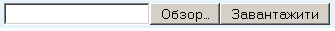
\includegraphics[scale=1,width=8cm]{ch05-01.png}
\caption{Форма завантаження файлу}
\label{f5-1:image}
\end{figure}

Перш, ніж приступити до написання сценарію обробки \verb'multipart'-форми, потрібно відредагувати файл конфігурації \verb'php.ini', щоб дозволити завантаження файлів на сервер.

Конфігураційний файл PHP php.ini має три параметри, пов'язані з завантаженням файлів на сервер:
\begin{enumerate}
\item \verb'file_uploads = On'~--- дозволяє завантаження файлів на сервер по протоколу HTTP;
\item \verb'upoad_tmp_dir = /tmp'~--- встановлює каталог для тимчасового зберігання завантажених файлів;
\item \verb'upload_max_filesize = 2M'~--- встановлює максимальний обсяг завантажуваних файлів. 

\end{enumerate}

Для успішного завантаження та збереження файлу необхідно створити сценарій виду:


\begin{lstlisting}[caption=Завантаження файлу на сервер]
<html>
<head>
  <title> Результат завантаження файлу </title>
</head>
<body>
<?php
if($_FILES["filename"]["size"] > 1024*3*1024)
   {
   echo ("Розмір файлу перевищує три мегабайта");
   exit;
   }
// Перевіряємо	чи	завантажився	файл
if(is_uploaded_file($_FILES["filename"]["tmp_name"]))
   {
   // Якщо так, то переносимо його у кінцевий каталог
   move_uploaded_file($_FILES["filename"]["tmp_name"], 
   "/path/to/file/".$_FILES["filename"]["name"]);
   } 
else 
   {
   echo("Помилка завантаження");
   }
?>
</body></html>
\end{lstlisting}

Слід зауважити, що для доступу до файлу використовується суперглобальний масив \verb'$_FILES', детальний опис якого дано у додатку~\ref{sup-glob:app}.



 
\pagebreak[3]
\section{Індивідуальне завдання}

\nopagebreak[4]
\subsection*{Завдання до лабораторної роботи}
\nopagebreak[4]
\begin{enumerate}
\item Вивчити теоретичний матеріал
\item Відповісти на контрольні запитання
\item Скласти алгоритм (блок-схему) програми
\item Виконати практичне завдання
\item Скласти звіт
\item Захистити роботу
\end{enumerate}

\subsection*{Контрольні запитання}
\nopagebreak[4]
\begin{enumerate}
\item Що таке файл? Що таке каталог?
\item Які основні операції для роботи з файлами ви знаєте?
\item Яким чином можна відкрити/створити файл у РНР?
\item Яким чином проводиться читання з файлу?
\item Яким чином проводиться запис у файл?
\item Яким чином можна переміщувати покажчик у файлі?
\item Що таке блокування файлу?
\item Які види блокування файлів ви знаєте?
\item Які особливості видів блокування файлів?
\item Яким чином завантажити файл на сервер?

\end{enumerate}

\subsection*{Практичні завдання}
\nopagebreak[4]


\begin{enumerate}
\item[]Створити форму з текстовим полем вводу для шляху каталогу та вивести таку інформацію: 
\item список об'єктів каталогу, підкаталоги виділити іншим кольором
\item вивести тільки файли, та реалізувати можливість їх видалення
\item знайти підкаталоги першого рівня та вивести їхній зміст
\item знайти порожні підкаталоги першого рівня, вивести їхні імена та видалити їх
\item створити 10 підкаталогів, та по 10 файлів у кожному, вивести отримане дерево
\item []Написати просту гостьову книгу, що зберігає інформацію у файлах, яка буде записувати та виводити:
\item перші 10 повідомлень користувачів та час відправлення
\item перші 10 повідомлень користувачів та поставлений ними рейтинг від 1 до 10
\item 10 повідомлень з найвищим рейтингом
\item список повідомлень з можливістю їх видалення
\item список повідомлень з можливістю їх редагування
\item[]Продемонструвати роботу гостьової книги 
\item[]Створити книгу рецептів, серед функцій якої є: 
\item виведення рецепту з найвищим рейтингом
\item виведення найсвіжіших рецептів
\item виведення найперших рецептів
\item збереження рецептів в окремих файлах
\item видалення вибраного рецепту
\item редагування вибраного рецепту
\item[]Продемонструвати роботу книги рецептів 
\item[]Створити фотогалерею з функціями додавання фотографії та опису до неї та додатковими функціями: 
\item виведення посилань на фото
\item виведення посилань на опис
\item виведення списку фото та видалення обраного
\item виведення списку та редагування опису обраного
\item обмежити розмір файлу, що завантажується до 1МБ
\item[]Продемонструвати роботу фотогалереї  
\item[]Створити файлове сховище з можливістю завантаження файлу та опису до нього та додатковими функціями:
\item вивести опис файлу та посилання для завантаження
\item реалізувати можливість видалення файлу
\item реалізувати можливість редагування імені файлу
\item реалізувати можливість редагування опису
\item[]Продемонструвати роботу файлового сховища 
\end{enumerate}


%\chapter{Сесії у РНР. Відправлення e-mail}
\section*{Мета роботи}
Навчитися використовувати сесії РНР та cookies. Розібратися в механізмі роботи сесій та cookies. Навчитися використовувати вбудовані засоби відправлення e-mail.
\section{Авторизація доступу}
У сучасних, навіть не дуже складних, веб-системах виникає потреба ідентифікувати користувача та виділити йому окреме поле діяльності. Якщо інформацію про ім'я, пароль та права користувача можна зберігати у файлах або у таблиці бази даних, то залишається проблема стеження за наявністю користувача на сайті.

Цю проблему можна вирішити двома способами:
\begin{itemize}
\item встановленням \verb'cookies'
\item запуском сесії.
\end{itemize}

Механізм сесій налаштований таким чином, що використовує механізм \verb'cookies' для передачі даних, але можливо обходитись і без \verb'cookies' у разі, коли вони відключені у користувача.
\section{Механізм сесії. Налаштування сесії}
\index{PHP!сесії}
\textbf{Сесія}~--- це механізм, який дозволяє створювати і використовувати змінні, зберігають своє значення протягом всього часу роботи користувача з сайтом.

Ці змінні для кожного користувача мають різні значення і можуть використовуватися на будь-якій сторінці сайту до виходу користувача з системи. При цьому кожного разу, заходячи на сайт, користувач отримує нові значення змінних, що дозволяють ідентифікувати його протягом цього сеансу або сесії роботи з сайтом. Звідси й назва механізму~--- сесії. 

Ідентифікатор сесії є 128 бітним числом. Якщо людина прийшла на сайт вперше і PHP-процесор це бачить, то даним відвідувачу присвоюється число, не присвоєне ще нікому. Надалі, при повторному заході, відвідувач буде асоційований з його особистим числом (ідентифікатором), через що програмі буде надана персональна область пам'яті.

Подання ідентифікатору сесії здійснюється у вигляді рядку із 32-х байт. Приклади ідентифікаторів сесії:

\begin{itemize}
\item \verb'7f4cbf53fbcd4717792447f32da7dba8'
\item \verb'ac4f4a45bdc893434c95dcaffb1c1811'
\end{itemize}

Налаштування PHP, в тому числі і для роботи з сесіями, прописуються у файлі \verb'php.ini'. В додатку~\ref{ses-opt:table} та~\ref{ses-opt-full:table} дано базові налаштування механізму сесії.

\subsection*{Унікальність сесій}
Підробити сесію або ідентифікатор не можна. Число з 128 біт (це 2 в 128 ступеня) в десятковому поданні має 38 нулів. Припустимо, на Вашому сайті буде 10~000 відвідувачів. Тоді у хакера шанси кілька зростають до 2 в ступені 114. Але це так само нереальна ймовірність~--- що-небудь підробити. Одна з очевидних причин наступна. Щоб підібрати номер сесії, потрібно зробити запит до Вашого веб-сервера. Нехай кожен запит займає 1024 байти. Через мільярд звернень до Вашого сайту, що складе 1000 ГБ трафіку, явно щось трапиться: Ваш сайт відключать через дикого трафіку або у вас не вистачить грошей на оплату такого великого трафіку. Ваш канал або пропускна здатність провайдера занадто слабка, щоб в розумні терміни перебрати всі номери. Ваш сервер не зможе хоч якось швидко працювати, маючи гігантську кількість пустих файлів, через створення фіктивних сесій. Ваш сервер переповниться лог-файлами і файлами фіктивних сесій, перестане працювати.

\subsection*{Збереження даних сесій}
Є два популярних способи зберігання даних сесій: база даних і файли. Ще можна зберігати сесії в пам'яті сервера (ОЗУ), але при виключенні сервера усі дані будуть втрачені. Зазвичай сесії зберігають у файлах, щоб знизити навантаження на базу даних. У деяких випадках сесії дозволяють повністю відмовитися від бази даних або використовувати її мінімально: в базі даних тільки список логінів/паролів, в сесіях (на файлах) вся робоча інформація.

За замовчуванням PHP зберігає всі в файлах (у своєму форматі) і сам дістає з них збережені дані. Після роботи кожного сценарію PHP сам все записує назад в особистий файл.

\subsection*{Передача ідентифікатора сесії}
Для передачі ідентифікатора сесії існують два основних способи і кілька маловживаних. Розглянемо скорочено механізм їх роботи:

\begin{enumerate}
\item \textbf{Cookies}

Це самий популярний і ефективний спосіб передачі ідентифікатора. Можна один раз помістити в куку змінну і всі інші скрипти будуть її отримувати. Якщо у користувача куки включені, PHP сам помістить туди ідентифікатор і потім сам його звідти дістане. 

Якщо у користувача куки вимкнені, то робота з сайтом може стати неможливою.

\item \textbf{параметри}
\begin{verse}
http://php.spb.ru/test.php?PHPSESSID=ac4f4a45bdc893434c95dcaffb1c1811
\end{verse}

Якщо ви будете дописувати всі ваші посилання подібним чином, то всі ваші наступні скрипти отримають ідентифікатор. PHP використовує і даний метод за замовчуванням (поєднуючи з куками, якщо ті вимкнені). Тобто PHP сам застосує або куки, або отриманий параметр.

Використання такого способу э 100\% надійним, але являється украй небезпечним, т.я. будь-хто може підробити параметр і отримати конфіденціальні дані користувача.

\item \textbf{PathInfo}
\begin{verse}
http://php.spb.ru/test.php/ac4f4a45bdc893434c95dcaffb1c1811
\end{verse}

Це засновано на розумінні веб-сервером того, де з цього URL шлях до скрипта, а де параметри. Тобто Апач розпізнає даний виклик, як звернення до файлу test.php і передасть йому рядок у змінній \verb'$pathinfo = getenv ("PATH_INFO")'. Відповідно, щоб передати управління в інший скрипт, треба подібним чином скласти URL (GET-запит) або передати форму GET або POST запитом.

\item Існують ще методи передачі ідентифікатора сесії, але вони ще менш зручні та не можуть надати надійного захисту від підробки.

\end{enumerate}



\section{Створення сесії, реєстрація змінних сесії, видалення змінних сесії}
\index{PHP!сесії!змінні сесії}
\index{PHP!функції!сесії}
При роботі із сесією виділяють три наступні етапи:
\begin{enumerate}
\item відкриття сесії
\item реєстрація змінних та їх використання
\item закриття сесії
\end{enumerate}
Нижче буде розглянуто всі три етапи.

\subsection*{Створення сесії}
Перше, що потрібно зробити для роботи з сесіями (якщо вони вже налаштовані адміністратором сервера), це запустити механізм сесій. Якщо в налаштуваннях сервера змінна \verb'session.auto_start = 0' (якщо \verb'session.auto_start = 1', то сесії запускаються автоматично), то будь-який скрипт, в якому потрібно використовувати дані сесії, повинен починатися з команди
\begin{verbatim}
  session_start(); 
\end{verbatim}

Отримавши таку команду, сервер створює нову сесію або відновлює поточну, ґрунтуючись на ідентифікаторі сесії, переданому за запитом.  Інтерпретатор PHP шукає змінну, в якій зберігається ідентифікатор сесії (за замовчуванням це \verb'PHPSESSID') спочатку в \verb'cookies', потім у змінних, переданих за допомогою \verb'POST' і \verb'GET'-запитів. Якщо ідентифікатор знайдений, то користувач вважається ідентифікованим, проводиться заміна всіх URL і виставляння \verb'cookies'. В іншому випадку користувач вважається новим, для нього генерується новий унікальний ідентифікатор, потім проводиться заміна URL і виставляння \verb'cookies'.

Нижче дано приклад роботи сесії:

\begin{verbatim}
<?
session_start(); 
echo session_id(); 
?>
<html>
<head><title>My home page</title></head>
... // домашняя страничка
</html>
<?
echo session_name(); 
?>
\end{verbatim}

Якщо оновити таку сторінку, то буде видно, що рядок, котрий друкує \verb'echo session_id();', не змінюється. Це вказує на те, що оновлення сесії проводиться успішно. Якщо закрити вікно браузера та відкрити цю сторінку знову, \verb'echo session_id();' видасть нове значення, томущо \verb'cookies' з минулої сесії вже знищено.


\subsection*{Реєстрація змінних}
Однак від самих ідентифікатора та імені сесії нам користі для вирішення завдань небагато. На практиці необхідно передавати щонайменше логін та пароль користувача. Для того щоб цього досягти, потрібно просто зареєструвати свої змінні:
\begin{verbatim}
session_register (ім'я_змінної1, 
        ім'я_змінної2, ...); 
\end{verbatim}
Зауважимо, що реєструються не значення, а імена змінних. Зареєструвати змінну досить один раз на будь-якій сторінці, де використовуються сесії. Імена змінних передаються функції \verb'session_register()' без знака <<\$>>. Всі зареєстровані таким чином змінні стають глобальними протягом даної сесії роботи з сайтом. 



\subsection*{Видалення змінних, сесії}
Крім вміння реєструвати змінні сесії (тобто робити їх глобальними протягом усього сеансу роботи), корисно також вміти видаляти такі змінні і сесію в цілому.

Функція \verb|session_unregister(ім'я_змінної)| видаляє глобальну змінну з поточної сесії (тобто видаляє її зі списку зареєстрованих змінних). Якщо реєстрація проводилася за допомогою \verb'$_SESSION', то використовують мовну конструкцію \verb'unset()'. Вона не повертає ніякого значення, а просто знищує зазначені змінні. Для того щоб скинути значення всіх змінних сесії, можна використовувати функцію \verb'session_unset();'.

Знищити поточну сесію цілком можна командою \verb'session_destroy();'. Вона не скидає значення глобальних змінних сесії і не видаляє \verb'cookies', а знищує всі дані, асоційовані з поточною сесією.

Перелік згаданих вище функцій дано у додатку~\ref{ses-func:text}. 
\section{Робота з cookies}
\index{PHP!cookies}

\textbf{Cookies}~--- це механізм зберігання даних браузером віддаленого комп'ютера для ідентифікації відвідувачів, що повертаються, та зберігання параметрів веб-сторінок (наприклад, змінних).

\textbf{Cookies}~--- це текстові рядки, що зберігаються на стороні клієнта, і містять пари <<ім'я-значення>>, з якими пов'язаний URL, по якому браузер визначає чи потрібно посилати \verb'cookies' на сервер.

Етапи роботи з  \verb'cookies' схожі на етапи використання механізму сесій:
\begin{enumerate}
\item встановлення \verb'cookies'
\item використання \verb'cookies'
\item видалення \verb'cookies'
\end{enumerate}
\subsection*{Встановлення cookies}
Встановлення cookies проводиться за допомогою функції \verb'setcookie()'. Ця функція має такі аргументи:
\begin{itemize}
\item \verb'name'~--- ім'я встановлюваного cookie;
\item \verb'value'~--- значення, яке зберігається в \verb'cookie' з ім'ям name;
\item \verb'expire'~--- час в секундах з початку епохи, по витікання якого поточний \verb'cookie' стає недійсним;
\item \verb'path'~--- шлях, по якому доступний cookie;
\item \verb'domain'~--- домен, з якого доступний cookie;
\item \verb'secure'~--- директива, яка визначає, чи доступний \verb'cookie' не по запиту HTPPS. За замовчуванням ця директива має значення 0, що означає можливість доступу до \verb'cookie' по звичайному запитом HTTP. 
\end{itemize}

При використанні Cookies необхідно мати на увазі, що Cookies повинні встановлюватися до першого виводу інформації в браузер (наприклад, оперетором echo або висновком якої функції). Тому бажано встановлювати Cookies на самому початку скрипта. Cookies встановлюються за допомогою певного заголовка сервера, а якщо скрипт виводить небудь, то це означає, що починається тіло документа. В результаті Cookies не будуть встановлені і може бути виведено попередження. Для перевірки успішності установки Cookies можна використовувати такий метод:

\begin{verbatim}
<?php
if (SetCookie("Test","Value")) 
echo "<h3>Cookies успішно встановлено!</h3>";
?>
\end{verbatim}

Функція \verb'SetCookie()' повертає TRUE у разі успішного встановлення Cookie. У разі, якщо Cookie встановити не вдається \verb'SetCookie()' поверне FALSE і можливо, попередження (залежить від налаштувань PHP). 


\subsection*{Використання cookies}

Доступ до \verb'cookie' здійснюється через суперглобальний масив \verb'$_COOKIE["name"]', де <<name>>~--- ім'я параметру, значення котрого необхідно отримати.

При читанні значень Cookies звертайте увагу на перевірку існування Cookies, наприклад, використовуючи оператор \verb'isset()'. Або шляхом придушення виведення помилок опереатором <<@>>.

Приклад встановлення Cookie і подальшого його читання:
\begin{verbatim}
<? php
setcookie( "test" , "Hello" , time()+3600 );
echo @$_COOKIE['test'];
?>
\end{verbatim}

У прикладі нижче показано як створити лічильник завантажень сторінки:
\begin{lstlisting}[caption=Лічильник завантажень сторінки]
<?php
// Проверяем, был ли уже установлен Cookie 'Mortal',
// Если да, то читаем его значение,
// И увеличиваем значение счетчика обращений к странице:
if (isset($_COOKIE['Mortal'])) $cnt=$_COOKIE['Mortal']+1;
else $cnt=0;
// Устанавливаем Cookie 'Mortal' зо значением счетчика,
// С временем "жизни" до 18/07/29,
// То есть на очень долгое время:
setcookie("Mortal",$cnt,0x6FFFFFFF);
// Выводит число посещений (загрузок) этой страницы:
echo "<p>Вы посещали эту страницу <b>".@$_COOKIE['Mortal']."</b> раз</p>";
?>
\end{lstlisting}

\subsection*{Встановлення масиву cookies}

Ми може встановити масив Cookies, використовуючи квадратні дужки в іменах Cookies \verb'[]', а потім прочитати масив Cookies і значення цього масиву:

\begin{lstlisting}[caption=Масив Cookies]
 <? php
// Устанавливаем массив Cookies:
setcookie("cookie[1]","Первый");
setcookie("cookie[2]","Второй");
setcookie("cookie[3]","Третий");
// После перезагрузки страницы мы отобразим
// Состав массива Cookies 'cookie':
if (isset($_COOKIE['cookie']))   
{
foreach ($_COOKIE ['cookie'] as $name => $value )   
   {
   echo "$name : $value <br>";
   }
}
?> 
\end{lstlisting}

\subsection*{Видалення cookies}

Іноді виникає необхідність видалення Cookies. Зробити це нескладно, необхідно лише знову встановити Cookie з ідентичним ім'ям і порожнім параметром. Наприклад:
\begin{verbatim}
<? php
SetCookie("Test" , "" );
?> 
\end{verbatim}


\section{Відправлення e-mail}
\index{PHP!функції!mail()}
\index{PHP!e-mail}
Найпростіший спосіб відправити лист за допомогою PHP~--- скористатися стандартною функцією \verb'mail()'. Вона має наступний синтаксис:
\begin{verbatim}
bool mail(to, subject, message [, additional\_headers 
[, additional\_parameters]])
\end{verbatim}

Обов'язкові параметри:
\begin{itemize}
\item E-mail одержувача
\item Заголовок листа
\item Текст листа 
\end{itemize}

Необов'язкові параметри:
\begin{itemize}
\item Додаткові заголовки листи
\item Додаткові параметри командного рядка 
\end{itemize}
Повертає значення:
\begin{itemize}
\item true, якщо лист було прийнято до доставки
\item false, в іншому випадку. 
\end{itemize}
Найпростіший приклад її використання виглядає так:
\begin{verbatim}
<?php
mail("joecool@example.com" , "My Subject" , "Line 1\nLine 2\nLine 3" );
?>
\end{verbatim}
Якщо у Вас на екрані з'явилася помилка <<Fatal error: Call to undefined function: mail()>>, це означає, що або PHP зібраний без підтримки функції mail, або вона заборонена налаштуваннями сервера. Така практика останнім часом широко поширена на безкоштовних хостингових серверах. Якщо Ви зіткнулися з такою проблемою, скористайтеся можливістю відправки листів за допомогою сокетів (sockets). 


\section{Альтернатива <<mail()>>}
\index{Системні додатки!sendmail}
На сьогоднішній день поширені наступні способи відправки листів з php-скриптів:
\begin{enumerate}
\item За допомогою виклику функції mail
\item Безпосередньо викликом sendmail
\item За допомогою сокетів
\item Використовуючи COM-об'єкт 
\end{enumerate}
\subsection*{sendmail}
\begin{lstlisting}[caption=Використання sendmail]
<?php
$sendmail = "/usr/sbin/sendmail -t -f $sender -C /etc/sendmail.orig.cf";
$fd = popen($sendmail, "w");
fputs($fd, "To: recipient@example.com\r\n");
fputs($fd, "From: \"Sender Name\" <$sender>\r\n");
fputs($fd, "Subject: Finally\r\n");
fputs($fd, "X-Mailer: Mailer Name\r\n\r\n");
fputs($fd, $body);
pclose($fd);
?> 
\end{lstlisting}
\subsection*{Active-X (COM)}
\begin{lstlisting}[caption=Використання Active-X]
<?php
@$CDONTS = new COM("CDONTS.NewMail");

@$CDONTS->From = "from_user@domain.com";
@$CDONTS->To = "to_user@domain.com";
@$CDONTS->CC = "cc_user@domain.com";
@$CDONTS->BCC = "bcc_user@domain.com";

@$CDONTS->BodyFormat = 0;
@$CDONTS->MailFormat = 0;

//@$CDONTS->AttachFile("c:\file.txt");

@$CDONTS->Subject = "Using CDONTS with PHP4 and IIS";
@$CDONTS->Body = "Blah blah blah blah, bleh...";

@$CDONTS->Send();
@$CDONTS->Close();
?> 
\end{lstlisting}

У разі роботи з сокетом відправлення дещо ускладнюється. Роботу з сокетами буде розглянуто в наступних лабораторних роботах.

\pagebreak[3]
\section{Індивідуальне завдання}

\nopagebreak[4]
\subsection*{Завдання до лабораторної роботи}
\nopagebreak[4]
\begin{enumerate}
\item Вивчити теоретичний матеріал
\item Відповісти на контрольні запитання
\item Скласти алгоритм (блок-схему) програми
\item Виконати практичне завдання
\item Скласти звіт
\item Захистити роботу
\end{enumerate}

\subsection*{Контрольні запитання}
\nopagebreak[4]
\begin{enumerate}
\item Що таке сесії? Для чого вони потрібні?
\item Яким чином забезпечується унікальність сесій?
\item Де зберігаються дані сесії?
\item Як створити сесію? 
\item Яким чином додати та видалити змінну сесії?
\item Що таке cookies?
\item Як використовувати cookies?
\item Як створити та використати масив cookies?
\item Яким чином можна відправити електронний лист?
\item Які альтернативи відправлень електронних листів ви знаєте?
\end{enumerate}

\subsection*{Практичні завдання}
\nopagebreak[4]


\begin{enumerate}
\item[]Написати HTML-сторінку з полями вводу логіну та паролю та додати наступний функціонал:
\item створити гостьову книгу, що зберігає запис користувача, виводить його записи, та дозволяє додавати нові без повторної авторизації
\item створити гостьову книгу що виводить перелік повідомлень та дозволяє видаляти їх певному користувачу без повторної авторизації
\item створити книгу рецептів, що дозволяє додавати, та дивитись додані рецепти тільки власнику записів послідовно без повторної авторизації
\item створити книгу рецептів, що дозволяє одному користувачу додавати рецепти, а іншому~--- видаляти
\item створити фотогалерею, що дозволяє додавати зображення та виводити їх перелік без повторної авторизації
\item створити фотогалерею, що дозволяє додавати зображення та видаляти їх певному користувачу без повторної авторизації
\item створити декілька зв'язаних сторінок, для різних користувачів виводити різну інформацію
\item створити примітивний форум на кілька користувачів (авторизація, додавання повідомлення, виведення повідомлень та імен користувачів)
\item створити сайт зі статтями, дати можливість просмотру неавторизованим користувачам та додавання авторизованим
\item створити сайт за статтями, дати можливість певним користувачам видаляти їх, заборонити просмотр неавторизованим користувачам
\item створити примітивний форум на кілька користувачів (авторизація, додавання повідомлення, виведення повідомлень та імен користувачів), що працює виключно на cookies
\item створити гостьову книгу, що зберігає запис користувача, виводить його записи, та дозволяє додавати нові без повторної авторизації, книга працює виключно на cookies
\item створити книгу рецептів, що дозволяє одному користувачу додавати рецепти, а іншому~--- видаляти, книга працює виключно на cookies
\item створити фотогалерею, що дозволяє додавати зображення та виводити їх перелік без повторної авторизації, фотогалерею працює виключно на cookies
\item створити примітивний онлайн-щоденник (додавання записів, виведення списку записів)
\item створити примітивний онлайн-щоденник (додавання записів, виведення списку записів), авторизацію користувача проводити за допомогою cookies
\item створити простий калькулятор (<<+>>, <<->>, <<*>>, <</>>) та виводити історію користувацьких обчислень 
\item створити простий калькулятор (<<+>>, <<->>, <<*>>, <</>>) та виводити історію користувацьких обчислень, авторизацію користувача проводити за допомогою cookies
\item створити гостьову книгу що виводить перелік повідомлень та дозволяє видаляти їх певному користувачу без повторної авторизації, авторизацію користувача проводити за допомогою cookies
\item створити простий калькулятор (<<+>>, <<->>, <<*>>, <</>>), записувати історію обчислень та виводити її адміністратору сайту
\item створити сторінку, що виводить адміністратору логін та пароль користувачів, та дозволяє їх змінювати 
\item створити сторінку, що виводить адміністратору логін та привілеї користувача, та дає право надавати права адміністратора
\item створити сторінку, яка дозволяє адміністратору видаляти користувачів з системи
\item створити сторінку, яка дозволяє додавати користувачів в систему
\item  створити фотогалерею, що дозволяє додавати зображення та видаляти їх певному користувачу без повторної авторизації, авторизацію користувача проводити за допомогою cookies
\item[]Результати роботи виводити у браузері.

\end{enumerate}



\chapter{Взаємодія РНР з СКБД MySQL}
\section*{Мета роботи}
Навчитися працювати з СУБД MySQL, записувати та отримувати табличні дані. Опрацювати взаємодію мови РНР з СУБД MySQL.

\section{Мова запитів SQL, та типи даних у СУБД MySQL}
\index{MySQL!SQL}
\subsection*{Основні команди}
Команди SQL можна поділити на дві категорії:
\begin{itemize}
\item команди означення даних
\item команди обробки даних
\end{itemize}

Перша категорія команд відповідає за створення або видалення баз даних, таблиць баз даних, редагування структури таблиць та типів даних полів таблиць.
До цієї категорії належать наступні команди:

\begin{itemize}
\item CREATE
\item DROP
\item ALTER
\item RENAME
\end{itemize}

Друга категорія команд відповідає за внесення даних до таблиць, оновлення та видалення даних.
До цієї категорії належать наступні команди:

\begin{itemize}
\item SELECT
\item INSERT
\item DELETE
\item UPDATE
\item HANDLER
\item TRUNCATE
\item REPLACE
\item LOAD DATA INFILE
\item DO
\end{itemize}

Нижче більш детально розглянуто синтаксис команд.

\subsection*{Команди означення даних}
\subsubsection*{CREATE}
\index{MySQL!SQL!CREATE}
Для створення бази даних необхідно використати наступну послідовність команд:

\begin{verbatim}
CREATE DATABASE [IF NOT EXISTS] db_name
\end{verbatim}

Оператор \verb'CREATE DATABASE' створює базу даних з вказаним іменем. Якщо база даних вже існує і не зазначений ключовий параметр \verb'IF NOT EXISTS', то виникає помилка виконання команди. 

Скорочений вид синтаксису команди створення таблиці виглядає наступним чином:

\begin{verbatim}
 CREATE [TEMPORARY] TABLE [IF NOT EXISTS] 
 tbl_name [(create_definition, ...)]
 [Table_options] [select_statement]
\end{verbatim}

Оператор створює таблицю. Якщо таблиця вже існує і не зазначений параметр \verb'IF NOT EXISTS', то виникає помилка виконання команди. Параметри таблиці та перелік полів вказують після означення імені таблиці. Приклад створення таблиці надано нижче:
\begin{verbatim}
 CREATE TABLE table123 (f1 INT, f2 INT)
\end{verbatim}
Створюється таблиця з двома полями цілочисельного типу.

Повний перелік можливих параметрів команди дано у додатку~\ref{crtab:text}.

Для створення індексів у СУБД MySQL існує команда CREATE INDEX. Синтаксис команди надано нижче: 
\begin{verbatim}
 CREATE [UNIQUE | FULLTEXT] INDEX index_name
         ON tbl_name (col_name [(length)], ...)
\end{verbatim}
Команда CREATE INDEX у версіях MySQL до 3.22 не виконує ніяких дій. У версії 3.22 і більш пізніх CREATE INDEX відповідає команді ALTER TABLE в частині створення індексів. Зазвичай всі індекси створюються в таблиці під час створення самої таблиці командою CREATE TABLE. CREATE INDEX дає можливість додати індекси до існуючих таблиць.


\subsubsection*{DROP}
\index{MySQL!SQL!DROP}
Для видалення бази даних існує наступна команда:
\begin{verbatim}
 DROP DATABASE [IF EXISTS] db_name
\end{verbatim}
Оператор DROP DATABASE видаляє всі таблиці в зазначеній базі даних і саму базу. Якщо ви виконуєте DROP DATABASE на базі даних, символічно пов'язаної з іншою, то видаляється як посилання, так і оригінальна база даних. Будьте дуже уважні при роботі з цією командою!

Оператор DROP DATABASE повертає кількість файлів, які були видалені з директорії бази даних. Як правило, це число дорівнює кількості таблиць, помноженому на три, оскільки зазвичай кожна таблиця представлена трьома файлами: .MYD-файлом, MYI-файлом і .Frm-файлом.

Команда DROP DATABASE видаляє з директорії зазначеної бази даних всі файли з наступними розширеннями: <<.BAK>>, <<.DAT>>, <<.HSH>>, <<.ISD>>, <<.ISM>>, <<.ISM>>, <<.MRG>>, <<.MYD>>, <<.MYI>>, <<.Db>>, <<.Frm>>. 	

Всі піддиректорії, імена яких складаються з двох цифр (RAID-директорії), також видаляються.

У версії MySQL 3.22 і більш пізніх можна використовувати ключові слова IF EXISTS для попередження помилки, якщо зазначена база даних не існує. 

Щоб видалити таблицю з поточної бази даних необхідно виконати наступну команду: 
\begin{verbatim}
 DROP TABLE [IF EXISTS] tbl_name 
 [, tbl_name, ...] [RESTRICT | CASCADE]
\end{verbatim}
Оператор DROP TABLE видаляє одну або декілька таблиць. Всі табличні дані та визначення видаляються, так що будьте уважні при роботі з цією командою!

У версії MySQL 3.22 і більш пізніх можна використовувати ключові слова IF EXISTS , щоб попередити помилку, якщо зазначені таблиці не існують. 

Для видалення індексів з таблиць необхідно використати команду
\begin{verbatim}
 DROP INDEX index_name ON tbl_name
\end{verbatim}
Оператор DROP INDEX видаляє індекси, зазначені в index\_name з таблиці tbl\_name. DROP INDEX не виконує ніяких дій у версіях MySQL до 3.22. У версіях 3.22 і більш пізніх DROP INDEX відповідає команді ALTER TABLE в частині видалення індексів.
\subsubsection*{ALTER}
\index{MySQL!SQL!ALTER}
Скорочений синтаксис команди для зміни структури таблиць виглядає наступним чином:
\begin{verbatim}
 ALTER [IGNORE] TABLE tbl_name alter_spec 
 [, alter_spec ...]
\end{verbatim}
Оператор ALTER TABLE забезпечує можливість змінювати структуру існуючої таблиці. Наприклад, можна додавати або видаляти стовпці, створювати або знищувати індекси або перейменовувати стовпці або саму таблицю. Можна також змінювати коментар для таблиці та її тип.

Нижче надано приклади використання команди:

Для того щоб змінити тип стовпця з INTEGER на TINYINT NOT NULL (залишаючи ім'я колишнім) і змінити тип стовпця b з CHAR(10) на CHAR(20) з перейменуванням його з b на c :
\begin{verbatim}
ALTER TABLE t2 MODIFY a TINYINT NOT NULL, 
      CHANGE bc CHAR (20);
\end{verbatim}

Для того щоб додати індекс до стовпцю d і зробити стовпець a первинним ключем:
\begin{verbatim}
ALTER TABLE t2 ADD INDEX (d), ADD PRIMARY KEY (a);
\end{verbatim}

Повні дані щодо синтаксису ALTER TABLE дано в додатку~\ref{alttab:text}.

\subsubsection*{RENAME}
\index{MySQL!SQL!RENAME}
Для перейменування таблиць, починаючи з версії 3.22, введено команду RENAME TABLE.
\begin{verbatim}
 RENAME TABLE tbl_name TO new_tbl_name 
 [, tbl_name2 TO new_tbl_name2, ...]
\end{verbatim}
Операція перейменування повинна здійснюватися як атомарна, тобто при виконанні перейменування ніякому іншому потоку не дозволяється доступ до зазначених таблиць. Завдяки цьому можливе заміщення таблиці порожній таблицею:
\begin{verbatim}
 CREATE TABLE new_table (...);
 RENAME TABLE old_table TO backup_table, 
 new_table TO old_table;
\end{verbatim}
Перейменування проводиться зліва направо. Таким чином, для обміну іменами між двома таблицями необхідно виконати наступні дії:
\begin{verbatim}
 RENAME TABLE old_table TO backup_table,
         new_table TO old_table,
         backup_table TO new_table;
\end{verbatim}
Для двох баз даних, що знаходяться на одному і тому ж диску, можна також здійснювати обмін іменами:
\begin{verbatim}
 RENAME TABLE current_db.tbl_name 
 TO other_db.tbl_name;
\end{verbatim}
При виконанні команди RENAME не повинні мати місце заблоковані таблиці або активні транзакції. Необхідно також мати привілеї ALTER і DROP для початкової таблиці і привілеї CREATE і INSERT~--- для нової.

Якщо MySQL стикається з якою-небудь помилкою при перейменуванні декількох таблиць, то станеться зворотне перейменування для всіх перейменованих таблиць, щоб повернути все в початковий стан. 

\subsection*{Команди обробки даних}
\subsubsection*{SELECT}
\index{MySQL!SQL!SELECT}

Оператор SELECT має наступну структуру:
\begin{verbatim}
 SELECT [STRAIGHT_JOIN]
        [SQL_SMALL_RESULT] [SQL_BIG_RESULT] 
        [SQL_BUFFER_RESULT] [SQL_CACHE | SQL_NO_CACHE] 
        [SQL_CALC_FOUND_ROWS] [HIGH_PRIORITY]
        [DISTINCT | DISTINCTROW | ALL]
     select_expression, ...
     [INTO {OUTFILE | DUMPFILE} 
     'file_name' export_options]
     [FROM table_references
       [WHERE where_definition]
       [GROUP BY {unsigned_integer | 
       col_name | formula} [ASC | DESC], ...]
       [HAVING where_definition]
       [ORDER BY {unsigned_integer | 
       col_name | formula} [ASC | DESC], ...]
       [LIMIT [offset,] rows]
       [PROCEDURE procedure_name]
       [FOR UPDATE | LOCK IN SHARE MODE]]
\end{verbatim}
SELECT застосовується для вилучення рядків, вибраних з однієї або декількох таблиць. Вираз select\_expression задає стовпці, в яких необхідно проводити вибірку. Крім того, оператор SELECT можна використовувати для витягання рядків, обчислених без посилання якусь таблицю. Наприклад запит \verb'SELECT 1 + 1;' поверне значення <<2>>.

\subsubsection*{INSERT}
\index{MySQL!SQL!INSERT}
\begin{verbatim}
     INSERT [LOW_PRIORITY | DELAYED] 
         [IGNORE] [INTO] tbl_name [(col_name, ...)]
         VALUES (expression, ...), (...), ...
 або INSERT [LOW_PRIORITY | DELAYED] [IGNORE]
         [INTO] tbl_name [(col_name, ...)]
         SELECT ...
 або INSERT [LOW_PRIORITY | DELAYED] [IGNORE]
         [INTO] tbl_name
         SET col_name = expression, 
         col_name = expression, ...
\end{verbatim}
Оператор INSERT вставляє нові рядки в існуючу таблицю. Форма даної команди INSERT \dots VALUES вставляє рядки відповідно до точно зазначеними в команді значеннями. Форма INSERT \dots SELECT вставляє рядки, обрані з іншої таблиці або таблиць. Форма INSERT ... VALUES зі списком з декількох значень підтримується у версії MySQL 3.22.5 і більш пізніх. Синтаксис вираження col\_name=expression підтримується у версії MySQL 3.22.10 і більш пізніх. 

Команда INSERT \dots SELECT забезпечує можливість швидкого внесення великої кількості рядків у таблицю з однієї або більше таблиць.
\begin{verbatim}
 INSERT INTO tblTemp2 (fldID) 
         SELECT tblTemp1.fldOrder_ID 
         FROM tblTemp1
         WHERE tblTemp1.fldOrder_ID > 100;
\end{verbatim}

\subsubsection*{DELETE}
\index{MySQL!SQL!DELETE}
\begin{verbatim}
DELETE [LOW_PRIORITY | QUICK] FROM table_name
       [WHERE where_definition]
       [ORDER BY ...]
       [LIMIT rows]

или

DELETE [LOW_PRIORITY | QUICK] table_name[.*] [,table_name[.*] ...]
       FROM table-references
       [WHERE where_definition]

oили

DELETE [LOW_PRIORITY | QUICK]
       FROM table_name[.*], [table_name[.*] ...]
       USING table-references
       [WHERE where_definition]
\end{verbatim}
Оператор DELETE видаляє з таблиці table\_name рядки, що задовольняють заданим в where\_definition умовам, і повертає число віддалених записів.

Якщо оператор DELETE запускається без визначення WHERE, то видаляються всі рядки. При роботі в режимі AUTOCOMMIT це буде аналогічно використанню оператора TRUNCATE. В MySQL 3.23 оператор DELETE без визначення WHERE поверне нуль як число віддалених записів.
\subsubsection*{UPDATE}
\index{MySQL!SQL!UPDATE}

\begin{verbatim}
UPDATE [LOW_PRIORITY] [IGNORE] tbl_name
    SET col_name1=expr1 [, col_name2=expr2, ...]
    [WHERE where_definition]
    [LIMIT #]
\end{verbatim}
Оператор UPDATE оновлює стовпці відповідно до їх новими значеннями в рядках існуючої таблиці. У виразі SET вказується, які саме стовпці слід модифікувати і які величини повинні бути в них встановлені. У виразі WHERE, якщо воно присутнє, задається, які рядки підлягають оновленню. В інших випадках оновлюються всі рядки. Якщо задано вираз ORDER BY, то рядки будуть оновлюватися у зазначеному в ньому порядку.

Якщо вказується ключове слово LOW\_PRIORITY, то виконання даної команди UPDATE затримується до тих пір, поки інші клієнти не завершать читання цієї таблиці.

Якщо вказується ключове слово IGNORE, то команда оновлення не буде перервана, навіть якщо при оновленні виникне помилка дублювання ключів. Рядки, через які виникають конфліктні ситуації, оновлені не будуть.

Якщо доступ до стовпцю із зазначеного виразу здійснюється по аргументу tbl\_name, то команда UPDATE використовує для цього стовпця його поточне значення.
\subsubsection*{HANDLER}
\index{MySQL!SQL!HANDLER}
Оператор HANDLER забезпечує прямий доступ до інтерфейсу дескриптора таблиці MyISAM, минаючи оптимізатор SQL. Отже, цей оператор працює швидше, ніж SELECT.

Перша форма оператора HANDLER відкриває таблицю, роблячи її доступною для послідовності команд HANDLER \dots READ. Цей об'єкт недоступний іншим потокам і не буде закритий, поки даний потік не викличе HANDLER tbl\_name CLOSE або сам потік не буде знищений.

Друга форма вибирає один рядок (або більше - у відповідності з установкою в вираженні LIMIT), для якої (их) зазначений індекс відповідає заданій умові і умова в виразі WHERE також виконується. Якщо індекс складається з декількох частин (охоплює декілька стовпців), то складові його величини вказуються у вигляді розділеного комами списку. Забезпечуються величини тільки для декількох перших шпальт.

Третя форма вибирає один рядок (або більше - у відповідності з установкою в вираженні LIMIT), з таблиці; гаразд вказівки індексів у відповідності з умовою WHERE.

Четверта форма (без зазначення індексів) вибирає один рядок (або більше - у відповідності з установкою в вираженні LIMIT), з таблиці, використовуючи природний порядок рядків (як вони зберігаються у файлі даних), у відповідності з умовою WHERE. Ця форма працює швидше, ніж HANDLER tbl\_name READ index\_name, в тих випадках, коли бажаний перегляд всієї таблиці.

Оператор HANDLER \dots CLOSE закриває таблицю, відкриту оператором HANDLER ... OPEN.
\subsubsection*{TRUNCATE}
\index{MySQL!SQL!TRUNCATE}
\begin{verbatim}
TRUNCATE TABLE table_name
\end{verbatim}
TRUNCATE TABLE має наступні відмінності від DELETE FROM ...:
\begin{itemize}
\item Ця операція видаляє і відтворює таблицю, що набагато швидше, ніж почергове видалення рядків.
\item Операція є нетранзакціонной; якщо одночасно виконується транзакція або активна блокування таблиці, то можна отримати помилку.
\item Не повертає кількість вилучених рядків.
\item Поки існує коректний файл <<table\_name.frm>>, таблицю можна відтворити з його допомогою, навіть якщо файли даних або індексів пошкоджені.
\end{itemize}

TRUNCATE є розширенням Oracle SQL.
\subsubsection*{REPLACE}
\index{MySQL!SQL!REPLACE}
\begin{verbatim}
    REPLACE [LOW_PRIORITY | DELAYED]
        [INTO] tbl_name [(col_name,...)]
        VALUES (expression,...),(...),...
или REPLACE [LOW_PRIORITY | DELAYED]
        [INTO] tbl_name [(col_name,...)]
        SELECT ...
или REPLACE [LOW_PRIORITY | DELAYED]
        [INTO] tbl_name
        SET col_name=expression, col_name=expression,...
\end{verbatim}

Оператор REPLACE працює точно так само, як INSERT, за винятком того, що якщо стара запис у даній таблиці має те ж значення індексу UNIQUE або PRIMARY KEY, що і нова, то стара запис перед занесенням нової буде видалена.

\subsubsection*{LOAD DATA INFILE}
\index{MySQL!SQL!LOAD DATA INFILE}

\begin{verbatim}
LOAD DATA [LOW_PRIORITY | CONCURRENT] [LOCAL] INFILE 'file_name.txt'
    [REPLACE | IGNORE]
    INTO TABLE tbl_name
    [FIELDS
        [TERMINATED BY '\t']
        [[OPTIONALLY] ENCLOSED BY '']
        [ESCAPED BY '\\' ]
    ]
    [LINES TERMINATED BY '\n']
    [IGNORE number LINES]
    [(col_name,...)]
\end{verbatim}

Команда LOAD DATA INFILE читає рядки з текстового файлу і вставляє їх у таблицю з дуже високою швидкістю. Якщо задано ключове слово LOCAL, то файл читається з клієнтського хоста. Якщо ж LOCAL не вказується, то файл повинен знаходитися на сервері. (Опція LOCAL доступна у версії MySQL 3.22.6 і більш пізніх.)

Якщо текстові файли, які потрібно прочитати, знаходяться на сервері, то з міркувань безпеки ці файли повинні або розміщуватися в директорії бази даних, або бути доступними для читання всім користувачам. Крім того, для застосування команди LOAD DATA INFILE до серверних файлів необхідно володіти привілеями FILE для серверного хосту.


\subsubsection*{DO}
\index{MySQL!SQL!DO}

\begin{verbatim}
DO expression, [expression, ...]
\end{verbatim}
Виконує даний вираз, але не повертає небудь результат. Є скороченою формою оператора SELECT expression, expression, але перевага його полягає в тому, що він працює трохи швидше, якщо немає необхідності в поверненні результату.

Оператор головним чином корисний при використанні з функціями, які мають побічні ефекти, такими як RELEASE\_LOCK.
\section{Функції для роботи з MySQL. Виконання SQL-запитів}
\index{MySQL!PHP!функції}

\section{Установка з'єднання. Вибір бази даних}
\index{MySQL!таблиці}

\section{Вибірка з таблиці, розбір результату вибірки}
\index{MySQL!вибірка}

\section{Додавання записів, оновлення записів}
\index{MySQL!додавання}
\index{MySQL!оновлення}
\section{Очищення і видалення таблиць}
\index{MySQL!очищення таблиць}
\index{MySQL!видалення таблиць}
\pagebreak[3]
\section{Індивідуальне завдання}

\nopagebreak[4]
\subsection*{Завдання до лабораторної роботи}
\nopagebreak[4]
\begin{enumerate}
\item Вивчити теоретичний матеріал
\item Відповісти на контрольні запитання
\item Скласти алгоритм (блок-схему) програми
\item Виконати практичне завдання
\item Скласти звіт
\item Захистити роботу
\end{enumerate}

\subsection*{Контрольні запитання}
\nopagebreak[4]
\begin{enumerate}
\item Що таке рядки?
\item Яким чином можна задати рядковий літерал?
\item Яка особливість рядків у подвійних лапках?
\item Яка особливість синтаксису \verb'Heredoc'? 
\item Яким чином вивести HTML-код на веб-сторінці?
\item Що таке регулярні вирази?
\item Яка особливість метасимволу <<\verb'\'>>?
\item Для чого використвуються регулярні вирази?
\item Які функції для роботи з регулярними виразами ви знаєте?
\item Яким чином можна використовувати регулярні вирази в SQL-запитах?
\end{enumerate}

\subsection*{Практичні завдання}
\nopagebreak[4]


\begin{enumerate}
\item[]Написати HTML-сторінку з формою, що складається з:
\item однорядкового поля вводу, поля вводу пароля та кнопки відправлення форми.
\item 

\end{enumerate}


\chapter{ООП. Робота з XML}
\index{PHP!ООП}
Хоча РНР володіє загальними об'єктно-орієнтованими можливостями, він не є повноцінною ОО-мовою (наприклад, такою, як C++ або Java). Зокрема, в РНР не підтримуються наступні об'єктно-орієнтовані можливості:
\begin{itemize}
\item множинне спадкування;
\item автоматичний виклик конструкторів (якщо ви хочете, щоб при конструюванні об'єкта похідного класу викликався конструктор базового класу, вам доведеться викликати його явно);
\item абстрактні класи;
\item перевантаження методів;
\item перевантаження операторів (це пов'язано з тим, що РНР є мовою з вільною типізацією);
закритий і відкритий доступ, віртуальні функції;
\item деструктори.
\end{itemize}

Але і без усього перерахованого ви все одно зможете отримати користь з об'єктно-орієнтованих можливостей, підтримуваних РНР. Реалізація ООП в РНР надає колосальну допомогу в модульному оформленні функціональності вашої програми.
\section{Класи та об'єкти. Методи}
\index{PHP!ООП!класи}
\index{PHP!ООП!об'єкти}
Класи утворюють синтаксичну базу об'єктно-орієнтованого програмування. Їх можна розглядати як свого роду <<контейнери>> для логічно пов'язаних даних і функцій (методів). Клас являє собою шаблон, по якому створюються конкретні екземпляри, використовуються в програмі. Екземпляри класів називаються об'єктами.

\subsection{Оголошення класу}
Клас можна розглядати як тип даних, а об'єкт~--- як змінну. Програма може одночасно працювати з декількома об'єктами одного класу як і з декількома змінними. Загальний формат класів РНР приведений в наступному лістингу.

\begin{lstlisting}[caption=Синтаксис оголошення класів]
class Class_name {
var $attribute_1;
//...
var $attribute_N;
function function1() {
//...
}
//...
function functionN() {
//...
}
} // end Class_name 
\end{lstlisting}

Оголошення класу має починатися з ключового слова \verb|class| (подібно до того, як оголошення функції починається з ключового слова \verb|function|). Кожному оголошенню атрибуту, що міститься в класі, має передувати ключове слово \verb|var|. Атрибути можуть відноситися до будь-якого типу даних, підтримуваних в РНР. Після оголошень атрибутів слідують оголошення методів, дуже схожі на типові оголошення функцій.

Методи часто використовуються для роботи з атрибутами класів. При посиланнях на атрибути всередині методів використовується спеціальна змінна \verb|$this|. Синтаксис методів продемонстрований в наступному прикладі:

\begin{lstlisting}[caption=Приклад створення методів]
<?
class Webpage {
var $bgcolor;
function setBgColor($color) {
$this->bgcolor = $color;
}
function getBgColor() {
return $this->bgcolor;
}
}
?> 
\end{lstlisting}

Змінна \verb|$this| посилається на екземпляр об'єкта, для якого викликається метод. Оскільки в будь-якому класі може існувати декілька екземплярів об'єктів, уточнення \verb|$this| необхідно для посилань на атрибути, що належать поточному об'єкту. При використанні цього синтаксису зверніть увагу на дві обставини:

\begin{enumerate}
\item атрибут, на який ви посилаєтеся в методі, не потрібно передавати у вигляді параметра функції;
\item знак долара (\$) ставиться перед змінною \verb|$this|, але не перед ім'ям атрибута (як у звичайної змінної).
\end{enumerate}

\subsection{Створення об'єкта}


\section{Наслідування}
\index{PHP!ООП!наслідування}

\section{Конструктори та деструктори}
\index{PHP!ООП!коснструктори}
\index{PHP!ООП!Деструктори}

Досить часто при створенні об'єкта потрібно задати значення деяких атрибутів. На щастя, розробники технології ООП врахували цю обставину і реалізували його в концепції конструкторів. Конструктор являє собою метод, який задає значення деяких атрибутів (а також може викликати інші методи). Конструктори викликаються автоматично при створенні нових об'єктів. Щоб це стало можливим, ім'я методу-конструктора повинне збігатися з ім'ям класу, в якому він міститься. Приклад конструктора приведений в лістингу 2.

\section{Оператори <<::>> та <<parent>>}
\index{PHP!ООП!<<::>>}
\index{PHP!ООП!<<parent>>}


\section{Об'єктна модель XML-документа}
\index{PHP!XML}
\section{Розширення SAX та DOM для роботы з XML}
\index{PHP!XML!SAX}
\index{PHP!XML!DOM}

\pagebreak[3]
\section{Індивідуальне завдання}

\nopagebreak[4]
\subsection*{Завдання до лабораторної роботи}
\nopagebreak[4]
\begin{enumerate}
\item Вивчити теоретичний матеріал
\item Відповісти на контрольні запитання
\item Скласти алгоритм (блок-схему) програми
\item Виконати практичне завдання
\item Скласти звіт
\item Захистити роботу
\end{enumerate}

\subsection*{Контрольні запитання}
\nopagebreak[4]
\begin{enumerate}
\item Що таке рядки?
\item Яким чином можна задати рядковий літерал?
\item Яка особливість рядків у подвійних лапках?
\item Яка особливість синтаксису \verb'Heredoc'? 
\item Яким чином вивести HTML-код на веб-сторінці?
\item Що таке регулярні вирази?
\item Яка особливість метасимволу <<\verb'\'>>?
\item Для чого використвуються регулярні вирази?
\item Які функції для роботи з регулярними виразами ви знаєте?
\item Яким чином можна використовувати регулярні вирази в SQL-запитах?
\end{enumerate}

\subsection*{Практичні завдання}
\nopagebreak[4]


\begin{enumerate}
\item[]Написати HTML-сторінку з формою, що складається з:
\item однорядкового поля вводу, поля вводу пароля та кнопки відправлення форми.
\item 

\end{enumerate}


\chapter{Робота з сокетами. Пересилання даних JSON}
\section{Структура сокета. Відкриття та закриття сокета}
\index{PHP!сокет}

\section{Запис в сокет та читання з сокета}
\section{Синтаксис JSON, його структура}
\index{JSON}

\section{Кодування та декодування JSON у РНР}
\index{JSON!PHP}
\index{PHP!JSON}
\section{Обмін даними з JavaScript-додатками}
\index{JSON!JavaScript}


\pagebreak[3]
\section{Індивідуальне завдання}

\nopagebreak[4]
\subsection*{Завдання до лабораторної роботи}
\nopagebreak[4]
\begin{enumerate}
\item Вивчити теоретичний матеріал
\item Відповісти на контрольні запитання
\item Скласти алгоритм (блок-схему) програми
\item Виконати практичне завдання
\item Скласти звіт
\item Захистити роботу
\end{enumerate}

\subsection*{Контрольні запитання}
\nopagebreak[4]
\begin{enumerate}
\item Що таке рядки?
\item Яким чином можна задати рядковий літерал?
\item Яка особливість рядків у подвійних лапках?
\item Яка особливість синтаксису \verb'Heredoc'? 
\item Яким чином вивести HTML-код на веб-сторінці?
\item Що таке регулярні вирази?
\item Яка особливість метасимволу <<\verb'\'>>?
\item Для чого використвуються регулярні вирази?
\item Які функції для роботи з регулярними виразами ви знаєте?
\item Яким чином можна використовувати регулярні вирази в SQL-запитах?
\end{enumerate}

\subsection*{Практичні завдання}
\nopagebreak[4]


\begin{enumerate}
\item[]Написати HTML-сторінку з формою, що складається з:
\item однорядкового поля вводу, поля вводу пароля та кнопки відправлення форми.
\item 

\end{enumerate}

\chapter{Робота з зображеннями}
\index{PHP!зображення}
\index{PHP!GD}
\section{Створення зображень}
\section{Малювання простих геометричних фігур}
\section{Малювання тексту на зображенні}
\section{Зміна розміру зображення}
\section{Функції бібліотеки GD}


\pagebreak[3]
\section{Індивідуальне завдання}

\nopagebreak[4]
\subsection*{Завдання до лабораторної роботи}
\nopagebreak[4]
\begin{enumerate}
\item Вивчити теоретичний матеріал
\item Відповісти на контрольні запитання
\item Скласти алгоритм (блок-схему) програми
\item Виконати практичне завдання
\item Скласти звіт
\item Захистити роботу
\end{enumerate}

\subsection*{Контрольні запитання}
\nopagebreak[4]
\begin{enumerate}
\item Що таке рядки?
\item Яким чином можна задати рядковий літерал?
\item Яка особливість рядків у подвійних лапках?
\item Яка особливість синтаксису \verb'Heredoc'? 
\item Яким чином вивести HTML-код на веб-сторінці?
\item Що таке регулярні вирази?
\item Яка особливість метасимволу <<\verb'\'>>?
\item Для чого використвуються регулярні вирази?
\item Які функції для роботи з регулярними виразами ви знаєте?
\item Яким чином можна використовувати регулярні вирази в SQL-запитах?
\end{enumerate}

\subsection*{Практичні завдання}
\nopagebreak[4]


\begin{enumerate}
\item[]Написати HTML-сторінку з формою, що складається з:
\item однорядкового поля вводу, поля вводу пароля та кнопки відправлення форми.
\item 

\end{enumerate}

\appendix
\makeatletter
\gdef\thechapter{\@Asbuk\c@chapter}
\makeatother
\def\chaptername{Додаток}


\chapter{Правила оформлення звіту}
\section{Титульна сторінка лабораторної роботи}
%\begin{titlepage}
%\newpage

\hrulefill

\begin{center}
МІНІСТЕРСТВО ОСВІТИ І НАУКИ, МОЛОДІ ТА СПОРТУ УКРАЇНИ \\

ХЕРСОНСЬКИЙ НАЦІОНАЛЬНИЙ ТЕХНІЧНИЙ УНІВЕРСИТЕТ \\*

КАФЕДРА ІНФОРМАЦІЙНИХ ТЕХНОЛОГІЙ

\end{center}

\vspace{5em}

\begin{center}
\Large Звіт до лабораторної роботи \No 123 \\ з дисципліни <<Web-програмування>>
\end{center}

\vspace{2.5em}

\begin{center}
{\Large Тема: \textbf{<<Основи мережі Internet>>}}
\end{center}

\vspace{5em}





\begin{flushleft}
Виконав \\ст.групи хПР1 \hspace{\fill} Пупкін А.А. \\
\vspace{1em}
Перевірив \\ст.викладач \hspace{\fill} Іванов Б.Б.\\
\end{flushleft}

\vspace{\fill}

\begin{center}
Херсон 2012
\end{center}
\newpage
%\end{titlepage}
\section{Приклади блок-схем}
Правила виконання блок-схем задані наступними документами:
\begin{itemize}
\item ГОСТ 19.701-90. Схемы алгоритмов, программ, данных и систем. Условные обозначения и правила выполнения
\item ГОСТ 19.002-80. Схемы алгоритмов и программ. Правила выполнения
\item ГОСТ 19.003-80. Схемы алгоритмов и программ. Обозначения условные графические

\end{itemize}




\begin{longtable}[t]{|c|p{6em}|p{15em}|}

\caption{\space Основны елементи блок-схем} \label{bl-ch:table}\\
\hline

Найменування & Позначення & Призначення \\
\hline \endfirsthead
\caption*{\space Продовження} \\
\hline
Найменування & Позначення & Призначення \\
\hline \endhead
\hline \endfoot



Блок початок-кінець &  % Graphic for TeX using PGF
% Title: C:\Documents and Settings\Admin\Мои документы\Мои рисунки\Диаграмма1.dia
% Creator: Dia v0.97.2
% CreationDate: Sat Sep 08 10:27:27 2012
% For: Admin
% \usepackage{tikz}
% The following commands are not supported in PSTricks at present
% We define them conditionally, so when they are implemented,
% this pgf file will use them.
\ifx\du\undefined
  \newlength{\du}
\fi
\setlength{\du}{15\unitlength}
\begin{tikzpicture}
\pgftransformxscale{1.000000}
\pgftransformyscale{-1.000000}
\definecolor{dialinecolor}{rgb}{0.000000, 0.000000, 0.000000}
\pgfsetstrokecolor{dialinecolor}
\definecolor{dialinecolor}{rgb}{1.000000, 1.000000, 1.000000}
\pgfsetfillcolor{dialinecolor}
\pgfsetlinewidth{0.100000\du}
\pgfsetdash{}{0pt}
\pgfsetdash{}{0pt}
\pgfsetbuttcap
\pgfsetmiterjoin
\pgfsetlinewidth{0.100000\du}
\pgfsetbuttcap
\pgfsetmiterjoin
\pgfsetdash{}{0pt}
\definecolor{dialinecolor}{rgb}{1.000000, 1.000000, 1.000000}
\pgfsetfillcolor{dialinecolor}
\pgfpathmoveto{\pgfpoint{5.632500\du}{0.350000\du}}
\pgfpathlineto{\pgfpoint{8.362500\du}{0.350000\du}}
\pgfpathcurveto{\pgfpoint{8.739435\du}{0.350000\du}}{\pgfpoint{9.045000\du}{0.641015\du}}{\pgfpoint{9.045000\du}{1.000000\du}}
\pgfpathcurveto{\pgfpoint{9.045000\du}{1.358985\du}}{\pgfpoint{8.739435\du}{1.650000\du}}{\pgfpoint{8.362500\du}{1.650000\du}}
\pgfpathlineto{\pgfpoint{5.632500\du}{1.650000\du}}
\pgfpathcurveto{\pgfpoint{5.255565\du}{1.650000\du}}{\pgfpoint{4.950000\du}{1.358985\du}}{\pgfpoint{4.950000\du}{1.000000\du}}
\pgfpathcurveto{\pgfpoint{4.950000\du}{0.641015\du}}{\pgfpoint{5.255565\du}{0.350000\du}}{\pgfpoint{5.632500\du}{0.350000\du}}
\pgfusepath{fill}
\definecolor{dialinecolor}{rgb}{0.000000, 0.000000, 0.000000}
\pgfsetstrokecolor{dialinecolor}
\pgfpathmoveto{\pgfpoint{5.632500\du}{0.350000\du}}
\pgfpathlineto{\pgfpoint{8.362500\du}{0.350000\du}}
\pgfpathcurveto{\pgfpoint{8.739435\du}{0.350000\du}}{\pgfpoint{9.045000\du}{0.641015\du}}{\pgfpoint{9.045000\du}{1.000000\du}}
\pgfpathcurveto{\pgfpoint{9.045000\du}{1.358985\du}}{\pgfpoint{8.739435\du}{1.650000\du}}{\pgfpoint{8.362500\du}{1.650000\du}}
\pgfpathlineto{\pgfpoint{5.632500\du}{1.650000\du}}
\pgfpathcurveto{\pgfpoint{5.255565\du}{1.650000\du}}{\pgfpoint{4.950000\du}{1.358985\du}}{\pgfpoint{4.950000\du}{1.000000\du}}
\pgfpathcurveto{\pgfpoint{4.950000\du}{0.641015\du}}{\pgfpoint{5.255565\du}{0.350000\du}}{\pgfpoint{5.632500\du}{0.350000\du}}
\pgfusepath{stroke}
% setfont left to latex
\definecolor{dialinecolor}{rgb}{0.000000, 0.000000, 0.000000}
\pgfsetstrokecolor{dialinecolor}
\node at (6.997500\du,1.250000\du){Початок};
\pgfsetlinewidth{0.100000\du}
\pgfsetdash{}{0pt}
\pgfsetdash{}{0pt}
\pgfsetbuttcap
\pgfsetmiterjoin
\pgfsetlinewidth{0.100000\du}
\pgfsetbuttcap
\pgfsetmiterjoin
\pgfsetdash{}{0pt}
\definecolor{dialinecolor}{rgb}{1.000000, 1.000000, 1.000000}
\pgfsetfillcolor{dialinecolor}
\pgfpathmoveto{\pgfpoint{5.683333\du}{1.950000\du}}
\pgfpathlineto{\pgfpoint{8.416667\du}{1.950000\du}}
\pgfpathcurveto{\pgfpoint{8.794061\du}{1.950000\du}}{\pgfpoint{9.100000\du}{2.241015\du}}{\pgfpoint{9.100000\du}{2.600000\du}}
\pgfpathcurveto{\pgfpoint{9.100000\du}{2.958985\du}}{\pgfpoint{8.794061\du}{3.250000\du}}{\pgfpoint{8.416667\du}{3.250000\du}}
\pgfpathlineto{\pgfpoint{5.683333\du}{3.250000\du}}
\pgfpathcurveto{\pgfpoint{5.305939\du}{3.250000\du}}{\pgfpoint{5.000000\du}{2.958985\du}}{\pgfpoint{5.000000\du}{2.600000\du}}
\pgfpathcurveto{\pgfpoint{5.000000\du}{2.241015\du}}{\pgfpoint{5.305939\du}{1.950000\du}}{\pgfpoint{5.683333\du}{1.950000\du}}
\pgfusepath{fill}
\definecolor{dialinecolor}{rgb}{0.000000, 0.000000, 0.000000}
\pgfsetstrokecolor{dialinecolor}
\pgfpathmoveto{\pgfpoint{5.683333\du}{1.950000\du}}
\pgfpathlineto{\pgfpoint{8.416667\du}{1.950000\du}}
\pgfpathcurveto{\pgfpoint{8.794061\du}{1.950000\du}}{\pgfpoint{9.100000\du}{2.241015\du}}{\pgfpoint{9.100000\du}{2.600000\du}}
\pgfpathcurveto{\pgfpoint{9.100000\du}{2.958985\du}}{\pgfpoint{8.794061\du}{3.250000\du}}{\pgfpoint{8.416667\du}{3.250000\du}}
\pgfpathlineto{\pgfpoint{5.683333\du}{3.250000\du}}
\pgfpathcurveto{\pgfpoint{5.305939\du}{3.250000\du}}{\pgfpoint{5.000000\du}{2.958985\du}}{\pgfpoint{5.000000\du}{2.600000\du}}
\pgfpathcurveto{\pgfpoint{5.000000\du}{2.241015\du}}{\pgfpoint{5.305939\du}{1.950000\du}}{\pgfpoint{5.683333\du}{1.950000\du}}
\pgfusepath{stroke}
% setfont left to latex
\definecolor{dialinecolor}{rgb}{0.000000, 0.000000, 0.000000}
\pgfsetstrokecolor{dialinecolor}
\node at (7.050000\du,2.850000\du){Кінець};
\end{tikzpicture}
 & Елемент відображає вхід із зовнішнього середовища або вихід з неї (найбільш часте застосування - початок і кінець програми). \\
\hline
Блок обчислень & % Graphic for TeX using PGF
% Title: C:\Documents and Settings\Admin\Мои документы\Мои рисунки\Диаграмма1.dia
% Creator: Dia v0.97.2
% CreationDate: Sat Sep 08 10:36:26 2012
% For: Admin
% \usepackage{tikz}
% The following commands are not supported in PSTricks at present
% We define them conditionally, so when they are implemented,
% this pgf file will use them.
\ifx\du\undefined
  \newlength{\du}
\fi
\setlength{\du}{15\unitlength}
\begin{tikzpicture}
\pgftransformxscale{1.000000}
\pgftransformyscale{-1.000000}
\definecolor{dialinecolor}{rgb}{0.000000, 0.000000, 0.000000}
\pgfsetstrokecolor{dialinecolor}
\definecolor{dialinecolor}{rgb}{1.000000, 1.000000, 1.000000}
\pgfsetfillcolor{dialinecolor}
\definecolor{dialinecolor}{rgb}{1.000000, 1.000000, 1.000000}
\pgfsetfillcolor{dialinecolor}
\fill (5.050000\du,0.450000\du)--(5.050000\du,2.350000\du)--(9.050000\du,2.350000\du)--(9.050000\du,0.450000\du)--cycle;
\pgfsetlinewidth{0.100000\du}
\pgfsetdash{}{0pt}
\pgfsetdash{}{0pt}
\pgfsetmiterjoin
\definecolor{dialinecolor}{rgb}{0.000000, 0.000000, 0.000000}
\pgfsetstrokecolor{dialinecolor}
\draw (5.050000\du,0.450000\du)--(5.050000\du,2.350000\du)--(9.050000\du,2.350000\du)--(9.050000\du,0.450000\du)--cycle;
% setfont left to latex
\definecolor{dialinecolor}{rgb}{0.000000, 0.000000, 0.000000}
\pgfsetstrokecolor{dialinecolor}
\node at (7.050000\du,1.640000\du){a = a+b};
\end{tikzpicture}
 & Виконання однієї або кількох операцій, обробка даних будь-якого виду (зміна значення даних, форми подання, розташування). \\
\hline
Логічний блок & % Graphic for TeX using PGF
% Title: C:\Documents and Settings\Admin\Мои документы\Мои рисунки\Диаграмма1.dia
% Creator: Dia v0.97.2
% CreationDate: Sat Sep 08 10:37:50 2012
% For: Admin
% \usepackage{tikz}
% The following commands are not supported in PSTricks at present
% We define them conditionally, so when they are implemented,
% this pgf file will use them.
\ifx\du\undefined
  \newlength{\du}
\fi
\setlength{\du}{15\unitlength}
\begin{tikzpicture}
\pgftransformxscale{1.000000}
\pgftransformyscale{-1.000000}
\definecolor{dialinecolor}{rgb}{0.000000, 0.000000, 0.000000}
\pgfsetstrokecolor{dialinecolor}
\definecolor{dialinecolor}{rgb}{1.000000, 1.000000, 1.000000}
\pgfsetfillcolor{dialinecolor}
\definecolor{dialinecolor}{rgb}{1.000000, 1.000000, 1.000000}
\pgfsetfillcolor{dialinecolor}
\fill (7.032170\du,0.332600\du)--(8.980207\du,1.947224\du)--(7.032170\du,3.561848\du)--(5.084133\du,1.947224\du)--cycle;
\pgfsetlinewidth{0.100000\du}
\pgfsetdash{}{0pt}
\pgfsetdash{}{0pt}
\pgfsetmiterjoin
\definecolor{dialinecolor}{rgb}{0.000000, 0.000000, 0.000000}
\pgfsetstrokecolor{dialinecolor}
\draw (7.032170\du,0.332600\du)--(8.980207\du,1.947224\du)--(7.032170\du,3.561848\du)--(5.084133\du,1.947224\du)--cycle;
% setfont left to latex
\definecolor{dialinecolor}{rgb}{0.000000, 0.000000, 0.000000}
\pgfsetstrokecolor{dialinecolor}
\node at (7.032170\du,2.187224\du){a>0};
\end{tikzpicture}
 & Відображає рішення або функцію перемикача типу з одним входом і двома або більше альтернативними виходами, з яких тільки один може бути обраний після обчислення умов. \\
\hline
Зумовлений процес & % Graphic for TeX using PGF
% Title: C:\Documents and Settings\Admin\Мои документы\Мои рисунки\Диаграмма1.dia
% Creator: Dia v0.97.2
% CreationDate: Sat Sep 08 10:38:44 2012
% For: Admin
% \usepackage{tikz}
% The following commands are not supported in PSTricks at present
% We define them conditionally, so when they are implemented,
% this pgf file will use them.
\ifx\du\undefined
  \newlength{\du}
\fi
\setlength{\du}{15\unitlength}
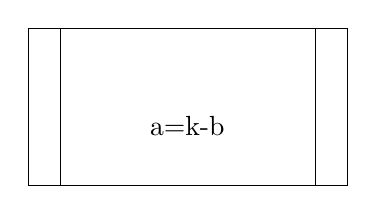
\begin{tikzpicture}
\pgftransformxscale{1.000000}
\pgftransformyscale{-1.000000}
\definecolor{dialinecolor}{rgb}{0.000000, 0.000000, 0.000000}
\pgfsetstrokecolor{dialinecolor}
\definecolor{dialinecolor}{rgb}{1.000000, 1.000000, 1.000000}
\pgfsetfillcolor{dialinecolor}
\pgfsetlinewidth{0.100000\du}
\pgfsetdash{}{0pt}
\pgfsetdash{}{0pt}
\pgfsetbuttcap
\pgfsetmiterjoin
\pgfsetlinewidth{0.100000\du}
\pgfsetbuttcap
\pgfsetmiterjoin
\pgfsetdash{}{0pt}
\definecolor{dialinecolor}{rgb}{1.000000, 1.000000, 1.000000}
\pgfsetfillcolor{dialinecolor}
\fill (5.000000\du,0.850000\du)--(5.000000\du,2.850000\du)--(9.050000\du,2.850000\du)--(9.050000\du,0.850000\du)--cycle;
\definecolor{dialinecolor}{rgb}{0.000000, 0.000000, 0.000000}
\pgfsetstrokecolor{dialinecolor}
\draw (5.000000\du,0.850000\du)--(5.000000\du,2.850000\du)--(9.050000\du,2.850000\du)--(9.050000\du,0.850000\du)--cycle;
\pgfsetbuttcap
\pgfsetmiterjoin
\pgfsetdash{}{0pt}
\definecolor{dialinecolor}{rgb}{0.000000, 0.000000, 0.000000}
\pgfsetstrokecolor{dialinecolor}
\draw (5.405000\du,0.850000\du)--(5.405000\du,2.850000\du);
\pgfsetbuttcap
\pgfsetmiterjoin
\pgfsetdash{}{0pt}
\definecolor{dialinecolor}{rgb}{0.000000, 0.000000, 0.000000}
\pgfsetstrokecolor{dialinecolor}
\draw (8.645000\du,0.850000\du)--(8.645000\du,2.850000\du);
% setfont left to latex
\definecolor{dialinecolor}{rgb}{0.000000, 0.000000, 0.000000}
\pgfsetstrokecolor{dialinecolor}
\node at (7.025000\du,2.100000\du){a=k-b};
\end{tikzpicture}
 & Символ відображає виконання процесу, що складається з однієї або декількох операцій, який визначений в іншому місці програми (в підпрограмі, модулі). \\
\hline
Дані & % Graphic for TeX using PGF
% Title: C:\Documents and Settings\Admin\Мои документы\Мои рисунки\Диаграмма1.dia
% Creator: Dia v0.97.2
% CreationDate: Sat Sep 08 10:40:01 2012
% For: Admin
% \usepackage{tikz}
% The following commands are not supported in PSTricks at present
% We define them conditionally, so when they are implemented,
% this pgf file will use them.
\ifx\du\undefined
  \newlength{\du}
\fi
\setlength{\du}{15\unitlength}
\begin{tikzpicture}
\pgftransformxscale{1.000000}
\pgftransformyscale{-1.000000}
\definecolor{dialinecolor}{rgb}{0.000000, 0.000000, 0.000000}
\pgfsetstrokecolor{dialinecolor}
\definecolor{dialinecolor}{rgb}{1.000000, 1.000000, 1.000000}
\pgfsetfillcolor{dialinecolor}
\definecolor{dialinecolor}{rgb}{1.000000, 1.000000, 1.000000}
\pgfsetfillcolor{dialinecolor}
\fill (5.818382\du,0.600000\du)--(8.950000\du,0.600000\du)--(8.222060\du,2.600000\du)--(5.090442\du,2.600000\du)--cycle;
\pgfsetlinewidth{0.100000\du}
\pgfsetdash{}{0pt}
\pgfsetdash{}{0pt}
\pgfsetmiterjoin
\definecolor{dialinecolor}{rgb}{0.000000, 0.000000, 0.000000}
\pgfsetstrokecolor{dialinecolor}
\draw (5.818382\du,0.600000\du)--(8.950000\du,0.600000\du)--(8.222060\du,2.600000\du)--(5.090442\du,2.600000\du)--cycle;
% setfont left to latex
\definecolor{dialinecolor}{rgb}{0.000000, 0.000000, 0.000000}
\pgfsetstrokecolor{dialinecolor}
\node at (7.020221\du,1.840000\du){x1, x2};
\end{tikzpicture}
 & Перетворення даних у форму, придатну для обробки (введення) або відображення результатів обробки (висновок). \\
\hline
Кордон циклу & % Graphic for TeX using PGF
% Title: C:\Documents and Settings\Admin\Мои документы\Мои рисунки\Диаграмма1.dia
% Creator: Dia v0.97.2
% CreationDate: Sat Sep 08 10:45:13 2012
% For: Admin
% \usepackage{tikz}
% The following commands are not supported in PSTricks at present
% We define them conditionally, so when they are implemented,
% this pgf file will use them.
\ifx\du\undefined
  \newlength{\du}
\fi
\setlength{\du}{15\unitlength}
\begin{tikzpicture}
\pgftransformxscale{1.000000}
\pgftransformyscale{-1.000000}
\definecolor{dialinecolor}{rgb}{0.000000, 0.000000, 0.000000}
\pgfsetstrokecolor{dialinecolor}
\definecolor{dialinecolor}{rgb}{1.000000, 1.000000, 1.000000}
\pgfsetfillcolor{dialinecolor}
\pgfsetlinewidth{0.100000\du}
\pgfsetdash{}{0pt}
\pgfsetdash{}{0pt}
\pgfsetbuttcap
\pgfsetmiterjoin
\pgfsetlinewidth{0.100000\du}
\pgfsetbuttcap
\pgfsetmiterjoin
\pgfsetdash{}{0pt}
\definecolor{dialinecolor}{rgb}{1.000000, 1.000000, 1.000000}
\pgfsetfillcolor{dialinecolor}
\pgfpathmoveto{\pgfpoint{5.479214\du}{0.850000\du}}
\pgfpathlineto{\pgfpoint{8.371536\du}{0.850000\du}}
\pgfpathlineto{\pgfpoint{8.950000\du}{1.625000\du}}
\pgfpathlineto{\pgfpoint{8.371536\du}{2.400000\du}}
\pgfpathlineto{\pgfpoint{5.479214\du}{2.400000\du}}
\pgfpathlineto{\pgfpoint{4.900750\du}{1.625000\du}}
\pgfpathlineto{\pgfpoint{5.479214\du}{0.850000\du}}
\pgfusepath{fill}
\definecolor{dialinecolor}{rgb}{0.000000, 0.000000, 0.000000}
\pgfsetstrokecolor{dialinecolor}
\pgfpathmoveto{\pgfpoint{5.479214\du}{0.850000\du}}
\pgfpathlineto{\pgfpoint{8.371536\du}{0.850000\du}}
\pgfpathlineto{\pgfpoint{8.950000\du}{1.625000\du}}
\pgfpathlineto{\pgfpoint{8.371536\du}{2.400000\du}}
\pgfpathlineto{\pgfpoint{5.479214\du}{2.400000\du}}
\pgfpathlineto{\pgfpoint{4.900750\du}{1.625000\du}}
\pgfpathlineto{\pgfpoint{5.479214\du}{0.850000\du}}
\pgfusepath{stroke}
% setfont left to latex
\definecolor{dialinecolor}{rgb}{0.000000, 0.000000, 0.000000}
\pgfsetstrokecolor{dialinecolor}
\node at (6.925375\du,1.875000\du){i=1;10;1};
\end{tikzpicture}
 & Символ складається з двох частин~--- відповідно, початок і кінець циклу - операції, що виконуються всередині циклу, розміщуються між ними. Умови циклу і збільшення записуються всередині символу початку або кінця циклу - в залежності від типу організації циклу. \\
\hline
З'єднувач & % Graphic for TeX using PGF
% Title: C:\Documents and Settings\Admin\Мои документы\Мои рисунки\Диаграмма1.dia
% Creator: Dia v0.97.2
% CreationDate: Sat Sep 08 10:46:12 2012
% For: Admin
% \usepackage{tikz}
% The following commands are not supported in PSTricks at present
% We define them conditionally, so when they are implemented,
% this pgf file will use them.
\ifx\du\undefined
  \newlength{\du}
\fi
\setlength{\du}{15\unitlength}
\begin{tikzpicture}
\pgftransformxscale{1.000000}
\pgftransformyscale{-1.000000}
\definecolor{dialinecolor}{rgb}{0.000000, 0.000000, 0.000000}
\pgfsetstrokecolor{dialinecolor}
\definecolor{dialinecolor}{rgb}{1.000000, 1.000000, 1.000000}
\pgfsetfillcolor{dialinecolor}
\definecolor{dialinecolor}{rgb}{1.000000, 1.000000, 1.000000}
\pgfsetfillcolor{dialinecolor}
\pgfpathellipse{\pgfpoint{6.147734\du}{1.633373\du}}{\pgfpoint{1.034541\du}{0\du}}{\pgfpoint{0\du}{0.961133\du}}
\pgfusepath{fill}
\pgfsetlinewidth{0.100000\du}
\pgfsetdash{}{0pt}
\pgfsetdash{}{0pt}
\pgfsetmiterjoin
\definecolor{dialinecolor}{rgb}{0.000000, 0.000000, 0.000000}
\pgfsetstrokecolor{dialinecolor}
\pgfpathellipse{\pgfpoint{6.147734\du}{1.633373\du}}{\pgfpoint{1.034541\du}{0\du}}{\pgfpoint{0\du}{0.961133\du}}
\pgfusepath{stroke}
% setfont left to latex
\definecolor{dialinecolor}{rgb}{0.000000, 0.000000, 0.000000}
\pgfsetstrokecolor{dialinecolor}
\node at (6.147734\du,1.873373\du){A};
\end{tikzpicture}
 & Символ відображає вхід в частину схеми і вихід з іншої частини цієї схеми.  \\
\hline
\end{longtable}

Приклад типової блок-схеми з вводом даних, розгалуженням, обчисленням та виводом даних дано на  малюнку~\ref{bl-ch:image}. 

\begin{figure}

\caption{Приклад нескладної блок-схеми}
% Graphic for TeX using PGF
% Title: C:\Documents and Settings\Admin\Мои документы\Мои рисунки\Диаграмма1.dia
% Creator: Dia v0.97.2
% CreationDate: Sat Sep 08 11:28:49 2012
% For: Admin
% \usepackage{tikz}
% The following commands are not supported in PSTricks at present
% We define them conditionally, so when they are implemented,
% this pgf file will use them.
\ifx\du\undefined
  \newlength{\du}
\fi
\setlength{\du}{15\unitlength}
\begin{tikzpicture}
\pgftransformxscale{1.000000}
\pgftransformyscale{-1.000000}
\definecolor{dialinecolor}{rgb}{0.000000, 0.000000, 0.000000}
\pgfsetstrokecolor{dialinecolor}
\definecolor{dialinecolor}{rgb}{1.000000, 1.000000, 1.000000}
\pgfsetfillcolor{dialinecolor}
\pgfsetlinewidth{0.100000\du}
\pgfsetdash{}{0pt}
\pgfsetdash{}{0pt}
\pgfsetbuttcap
\pgfsetmiterjoin
\pgfsetlinewidth{0.100000\du}
\pgfsetbuttcap
\pgfsetmiterjoin
\pgfsetdash{}{0pt}
\definecolor{dialinecolor}{rgb}{1.000000, 1.000000, 1.000000}
\pgfsetfillcolor{dialinecolor}
\pgfpathmoveto{\pgfpoint{4.983333\du}{0.725000\du}}
\pgfpathlineto{\pgfpoint{8.116667\du}{0.725000\du}}
\pgfpathcurveto{\pgfpoint{8.549290\du}{0.725000\du}}{\pgfpoint{8.900000\du}{1.004822\du}}{\pgfpoint{8.900000\du}{1.350000\du}}
\pgfpathcurveto{\pgfpoint{8.900000\du}{1.695178\du}}{\pgfpoint{8.549290\du}{1.975000\du}}{\pgfpoint{8.116667\du}{1.975000\du}}
\pgfpathlineto{\pgfpoint{4.983333\du}{1.975000\du}}
\pgfpathcurveto{\pgfpoint{4.550710\du}{1.975000\du}}{\pgfpoint{4.200000\du}{1.695178\du}}{\pgfpoint{4.200000\du}{1.350000\du}}
\pgfpathcurveto{\pgfpoint{4.200000\du}{1.004822\du}}{\pgfpoint{4.550710\du}{0.725000\du}}{\pgfpoint{4.983333\du}{0.725000\du}}
\pgfusepath{fill}
\definecolor{dialinecolor}{rgb}{0.000000, 0.000000, 0.000000}
\pgfsetstrokecolor{dialinecolor}
\pgfpathmoveto{\pgfpoint{4.983333\du}{0.725000\du}}
\pgfpathlineto{\pgfpoint{8.116667\du}{0.725000\du}}
\pgfpathcurveto{\pgfpoint{8.549290\du}{0.725000\du}}{\pgfpoint{8.900000\du}{1.004822\du}}{\pgfpoint{8.900000\du}{1.350000\du}}
\pgfpathcurveto{\pgfpoint{8.900000\du}{1.695178\du}}{\pgfpoint{8.549290\du}{1.975000\du}}{\pgfpoint{8.116667\du}{1.975000\du}}
\pgfpathlineto{\pgfpoint{4.983333\du}{1.975000\du}}
\pgfpathcurveto{\pgfpoint{4.550710\du}{1.975000\du}}{\pgfpoint{4.200000\du}{1.695178\du}}{\pgfpoint{4.200000\du}{1.350000\du}}
\pgfpathcurveto{\pgfpoint{4.200000\du}{1.004822\du}}{\pgfpoint{4.550710\du}{0.725000\du}}{\pgfpoint{4.983333\du}{0.725000\du}}
\pgfusepath{stroke}
% setfont left to latex
\definecolor{dialinecolor}{rgb}{0.000000, 0.000000, 0.000000}
\pgfsetstrokecolor{dialinecolor}
\node at (6.550000\du,1.600000\du){Початок};
\definecolor{dialinecolor}{rgb}{1.000000, 1.000000, 1.000000}
\pgfsetfillcolor{dialinecolor}
\fill (5.517353\du,3.325000\du)--(9.701029\du,3.325000\du)--(8.973089\du,5.325000\du)--(4.789413\du,5.325000\du)--cycle;
\pgfsetlinewidth{0.100000\du}
\pgfsetdash{}{0pt}
\pgfsetdash{}{0pt}
\pgfsetmiterjoin
\definecolor{dialinecolor}{rgb}{0.000000, 0.000000, 0.000000}
\pgfsetstrokecolor{dialinecolor}
\draw (5.517353\du,3.325000\du)--(9.701029\du,3.325000\du)--(8.973089\du,5.325000\du)--(4.789413\du,5.325000\du)--cycle;
% setfont left to latex
\definecolor{dialinecolor}{rgb}{0.000000, 0.000000, 0.000000}
\pgfsetstrokecolor{dialinecolor}
\node at (7.245221\du,4.565000\du){x1, x2, x3};
\definecolor{dialinecolor}{rgb}{1.000000, 1.000000, 1.000000}
\pgfsetfillcolor{dialinecolor}
\fill (6.869670\du,6.850000\du)--(9.985382\du,8.301957\du)--(6.869670\du,9.753914\du)--(3.753958\du,8.301957\du)--cycle;
\pgfsetlinewidth{0.100000\du}
\pgfsetdash{}{0pt}
\pgfsetdash{}{0pt}
\pgfsetmiterjoin
\definecolor{dialinecolor}{rgb}{0.000000, 0.000000, 0.000000}
\pgfsetstrokecolor{dialinecolor}
\draw (6.869670\du,6.850000\du)--(9.985382\du,8.301957\du)--(6.869670\du,9.753914\du)--(3.753958\du,8.301957\du)--cycle;
% setfont left to latex
\definecolor{dialinecolor}{rgb}{0.000000, 0.000000, 0.000000}
\pgfsetstrokecolor{dialinecolor}
\node at (6.869670\du,8.541957\du){x1<x2};
% setfont left to latex
\definecolor{dialinecolor}{rgb}{0.000000, 0.000000, 0.000000}
\pgfsetstrokecolor{dialinecolor}
\node[anchor=west] at (2.725000\du,7.725000\du){Так};
% setfont left to latex
\definecolor{dialinecolor}{rgb}{0.000000, 0.000000, 0.000000}
\pgfsetstrokecolor{dialinecolor}
\node[anchor=west] at (10.150000\du,7.750000\du){Ні};
\definecolor{dialinecolor}{rgb}{1.000000, 1.000000, 1.000000}
\pgfsetfillcolor{dialinecolor}
\fill (1.066250\du,10.050000\du)--(1.066250\du,12.000000\du)--(5.333750\du,12.000000\du)--(5.333750\du,10.050000\du)--cycle;
\pgfsetlinewidth{0.100000\du}
\pgfsetdash{}{0pt}
\pgfsetdash{}{0pt}
\pgfsetmiterjoin
\definecolor{dialinecolor}{rgb}{0.000000, 0.000000, 0.000000}
\pgfsetstrokecolor{dialinecolor}
\draw (1.066250\du,10.050000\du)--(1.066250\du,12.000000\du)--(5.333750\du,12.000000\du)--(5.333750\du,10.050000\du)--cycle;
% setfont left to latex
\definecolor{dialinecolor}{rgb}{0.000000, 0.000000, 0.000000}
\pgfsetstrokecolor{dialinecolor}
\node at (3.200000\du,11.265000\du){a = x1 - x3};
\definecolor{dialinecolor}{rgb}{1.000000, 1.000000, 1.000000}
\pgfsetfillcolor{dialinecolor}
\fill (9.000000\du,10.090000\du)--(9.000000\du,11.990000\du)--(13.678750\du,11.990000\du)--(13.678750\du,10.090000\du)--cycle;
\pgfsetlinewidth{0.100000\du}
\pgfsetdash{}{0pt}
\pgfsetdash{}{0pt}
\pgfsetmiterjoin
\definecolor{dialinecolor}{rgb}{0.000000, 0.000000, 0.000000}
\pgfsetstrokecolor{dialinecolor}
\draw (9.000000\du,10.090000\du)--(9.000000\du,11.990000\du)--(13.678750\du,11.990000\du)--(13.678750\du,10.090000\du)--cycle;
% setfont left to latex
\definecolor{dialinecolor}{rgb}{0.000000, 0.000000, 0.000000}
\pgfsetstrokecolor{dialinecolor}
\node at (11.339375\du,11.280000\du){a = x1 + x3};
\pgfsetlinewidth{0.100000\du}
\pgfsetdash{}{0pt}
\pgfsetdash{}{0pt}
\pgfsetbuttcap
\pgfsetmiterjoin
\pgfsetlinewidth{0.100000\du}
\pgfsetbuttcap
\pgfsetmiterjoin
\pgfsetdash{}{0pt}
\definecolor{dialinecolor}{rgb}{1.000000, 1.000000, 1.000000}
\pgfsetfillcolor{dialinecolor}
\fill (6.350000\du,13.950000\du)--(8.350000\du,13.950000\du)--(7.350000\du,16.150000\du)--cycle;
\definecolor{dialinecolor}{rgb}{0.000000, 0.000000, 0.000000}
\pgfsetstrokecolor{dialinecolor}
\draw (6.350000\du,13.950000\du)--(8.350000\du,13.950000\du)--(7.350000\du,16.150000\du)--cycle;
% setfont left to latex
\definecolor{dialinecolor}{rgb}{0.000000, 0.000000, 0.000000}
\pgfsetstrokecolor{dialinecolor}
\node at (7.350000\du,14.750000\du){};
\pgfsetlinewidth{0.100000\du}
\pgfsetdash{}{0pt}
\pgfsetdash{}{0pt}
\pgfsetbuttcap
\pgfsetmiterjoin
\pgfsetlinewidth{0.100000\du}
\pgfsetbuttcap
\pgfsetmiterjoin
\pgfsetdash{}{0pt}
\definecolor{dialinecolor}{rgb}{1.000000, 1.000000, 1.000000}
\pgfsetfillcolor{dialinecolor}
\pgfpathmoveto{\pgfpoint{6.128333\du}{20.940000\du}}
\pgfpathlineto{\pgfpoint{9.261667\du}{20.940000\du}}
\pgfpathcurveto{\pgfpoint{9.694290\du}{20.940000\du}}{\pgfpoint{10.045000\du}{21.219822\du}}{\pgfpoint{10.045000\du}{21.565000\du}}
\pgfpathcurveto{\pgfpoint{10.045000\du}{21.910178\du}}{\pgfpoint{9.694290\du}{22.190000\du}}{\pgfpoint{9.261667\du}{22.190000\du}}
\pgfpathlineto{\pgfpoint{6.128333\du}{22.190000\du}}
\pgfpathcurveto{\pgfpoint{5.695710\du}{22.190000\du}}{\pgfpoint{5.345000\du}{21.910178\du}}{\pgfpoint{5.345000\du}{21.565000\du}}
\pgfpathcurveto{\pgfpoint{5.345000\du}{21.219822\du}}{\pgfpoint{5.695710\du}{20.940000\du}}{\pgfpoint{6.128333\du}{20.940000\du}}
\pgfusepath{fill}
\definecolor{dialinecolor}{rgb}{0.000000, 0.000000, 0.000000}
\pgfsetstrokecolor{dialinecolor}
\pgfpathmoveto{\pgfpoint{6.128333\du}{20.940000\du}}
\pgfpathlineto{\pgfpoint{9.261667\du}{20.940000\du}}
\pgfpathcurveto{\pgfpoint{9.694290\du}{20.940000\du}}{\pgfpoint{10.045000\du}{21.219822\du}}{\pgfpoint{10.045000\du}{21.565000\du}}
\pgfpathcurveto{\pgfpoint{10.045000\du}{21.910178\du}}{\pgfpoint{9.694290\du}{22.190000\du}}{\pgfpoint{9.261667\du}{22.190000\du}}
\pgfpathlineto{\pgfpoint{6.128333\du}{22.190000\du}}
\pgfpathcurveto{\pgfpoint{5.695710\du}{22.190000\du}}{\pgfpoint{5.345000\du}{21.910178\du}}{\pgfpoint{5.345000\du}{21.565000\du}}
\pgfpathcurveto{\pgfpoint{5.345000\du}{21.219822\du}}{\pgfpoint{5.695710\du}{20.940000\du}}{\pgfpoint{6.128333\du}{20.940000\du}}
\pgfusepath{stroke}
% setfont left to latex
\definecolor{dialinecolor}{rgb}{0.000000, 0.000000, 0.000000}
\pgfsetstrokecolor{dialinecolor}
\node at (7.695000\du,21.815000\du){Початок};
\definecolor{dialinecolor}{rgb}{1.000000, 1.000000, 1.000000}
\pgfsetfillcolor{dialinecolor}
\fill (6.322940\du,17.390000\du)--(10.506617\du,17.390000\du)--(9.778676\du,19.390000\du)--(5.595000\du,19.390000\du)--cycle;
\pgfsetlinewidth{0.100000\du}
\pgfsetdash{}{0pt}
\pgfsetdash{}{0pt}
\pgfsetmiterjoin
\definecolor{dialinecolor}{rgb}{0.000000, 0.000000, 0.000000}
\pgfsetstrokecolor{dialinecolor}
\draw (6.322940\du,17.390000\du)--(10.506617\du,17.390000\du)--(9.778676\du,19.390000\du)--(5.595000\du,19.390000\du)--cycle;
% setfont left to latex
\definecolor{dialinecolor}{rgb}{0.000000, 0.000000, 0.000000}
\pgfsetstrokecolor{dialinecolor}
\node at (8.050808\du,18.630000\du){a};
\pgfsetlinewidth{0.100000\du}
\pgfsetdash{}{0pt}
\pgfsetdash{}{0pt}
\pgfsetmiterjoin
\pgfsetbuttcap
{
\definecolor{dialinecolor}{rgb}{0.000000, 0.000000, 0.000000}
\pgfsetfillcolor{dialinecolor}
% was here!!!
\pgfsetarrowsend{stealth}
{\pgfsetcornersarced{\pgfpoint{0.000000\du}{0.000000\du}}\definecolor{dialinecolor}{rgb}{0.000000, 0.000000, 0.000000}
\pgfsetstrokecolor{dialinecolor}
\draw (3.753958\du,8.301957\du)--(3.753958\du,8.300000\du)--(3.200000\du,8.300000\du)--(3.200000\du,10.050000\du);
}}
\pgfsetlinewidth{0.100000\du}
\pgfsetdash{}{0pt}
\pgfsetdash{}{0pt}
\pgfsetmiterjoin
\pgfsetbuttcap
{
\definecolor{dialinecolor}{rgb}{0.000000, 0.000000, 0.000000}
\pgfsetfillcolor{dialinecolor}
% was here!!!
\pgfsetarrowsend{stealth}
{\pgfsetcornersarced{\pgfpoint{0.000000\du}{0.000000\du}}\definecolor{dialinecolor}{rgb}{0.000000, 0.000000, 0.000000}
\pgfsetstrokecolor{dialinecolor}
\draw (9.985382\du,8.301957\du)--(9.985382\du,8.300000\du)--(11.339375\du,8.300000\du)--(11.339375\du,10.090000\du);
}}
\pgfsetlinewidth{0.100000\du}
\pgfsetdash{}{0pt}
\pgfsetdash{}{0pt}
\pgfsetmiterjoin
\pgfsetbuttcap
{
\definecolor{dialinecolor}{rgb}{0.000000, 0.000000, 0.000000}
\pgfsetfillcolor{dialinecolor}
% was here!!!
\pgfsetarrowsend{stealth}
{\pgfsetcornersarced{\pgfpoint{0.000000\du}{0.000000\du}}\definecolor{dialinecolor}{rgb}{0.000000, 0.000000, 0.000000}
\pgfsetstrokecolor{dialinecolor}
\draw (3.200000\du,12.000000\du)--(3.200000\du,12.975000\du)--(6.850000\du,12.975000\du)--(6.850000\du,13.950000\du);
}}
\pgfsetlinewidth{0.100000\du}
\pgfsetdash{}{0pt}
\pgfsetdash{}{0pt}
\pgfsetmiterjoin
\pgfsetbuttcap
{
\definecolor{dialinecolor}{rgb}{0.000000, 0.000000, 0.000000}
\pgfsetfillcolor{dialinecolor}
% was here!!!
\pgfsetarrowsend{stealth}
{\pgfsetcornersarced{\pgfpoint{0.000000\du}{0.000000\du}}\definecolor{dialinecolor}{rgb}{0.000000, 0.000000, 0.000000}
\pgfsetstrokecolor{dialinecolor}
\draw (11.339375\du,11.990000\du)--(11.339375\du,12.970000\du)--(7.850000\du,12.970000\du)--(7.850000\du,13.950000\du);
}}
\pgfsetlinewidth{0.100000\du}
\pgfsetdash{}{0pt}
\pgfsetdash{}{0pt}
\pgfsetbuttcap
{
\definecolor{dialinecolor}{rgb}{0.000000, 0.000000, 0.000000}
\pgfsetfillcolor{dialinecolor}
% was here!!!
\pgfsetarrowsend{stealth}
\definecolor{dialinecolor}{rgb}{0.000000, 0.000000, 0.000000}
\pgfsetstrokecolor{dialinecolor}
\draw (6.550000\du,1.975000\du)--(6.563272\du,3.325000\du);
}
\pgfsetlinewidth{0.100000\du}
\pgfsetdash{}{0pt}
\pgfsetdash{}{0pt}
\pgfsetbuttcap
{
\definecolor{dialinecolor}{rgb}{0.000000, 0.000000, 0.000000}
\pgfsetfillcolor{dialinecolor}
% was here!!!
\pgfsetarrowsend{stealth}
\definecolor{dialinecolor}{rgb}{0.000000, 0.000000, 0.000000}
\pgfsetstrokecolor{dialinecolor}
\draw (6.881251\du,5.325000\du)--(6.869670\du,6.850000\du);
}
\pgfsetlinewidth{0.100000\du}
\pgfsetdash{}{0pt}
\pgfsetdash{}{0pt}
\pgfsetbuttcap
{
\definecolor{dialinecolor}{rgb}{0.000000, 0.000000, 0.000000}
\pgfsetfillcolor{dialinecolor}
% was here!!!
\pgfsetarrowsend{stealth}
\definecolor{dialinecolor}{rgb}{0.000000, 0.000000, 0.000000}
\pgfsetstrokecolor{dialinecolor}
\draw (7.350000\du,16.150000\du)--(7.368860\du,17.390000\du);
}
\pgfsetlinewidth{0.100000\du}
\pgfsetdash{}{0pt}
\pgfsetdash{}{0pt}
\pgfsetbuttcap
{
\definecolor{dialinecolor}{rgb}{0.000000, 0.000000, 0.000000}
\pgfsetfillcolor{dialinecolor}
% was here!!!
\pgfsetarrowsend{stealth}
\definecolor{dialinecolor}{rgb}{0.000000, 0.000000, 0.000000}
\pgfsetstrokecolor{dialinecolor}
\draw (7.686838\du,19.390000\du)--(7.695000\du,20.940000\du);
}
\end{tikzpicture}

\label{bl-ch:image}
\end{figure} 


\section{Оформлення програмного коду}
Програмний код необхідно оформлювати у друкованому вигляді, бажано використовуючи моноширинний шрифт \verb'Сourier' або \verb'Сourier New' розміром 12~--~14pt. Приклад оформлення лістингів надано нижче.
\section{Оформлення скріншотів}
Скріншоти HTML-форм або PHP-сценаріїв бажано оформлювати без рамки веб-браузера по 1~--~2 зображення на сторінку. При використанні на фоні HTML-сторінки темних кольорів можливе редагування зображення з метою висвітлення кольорів. Приклад зображення, що отримано з комбінацій клавіш \verb'Alt+PrtCs' зображена на малюнку~\ref{prsc-orig:image}, та бажане зображення на малюнку малюнку~\ref{prsc-rel:image}. Небажане оформлення скріншота дано на  малюнку~\ref{prsc-bad:image}.

\begin{figure}
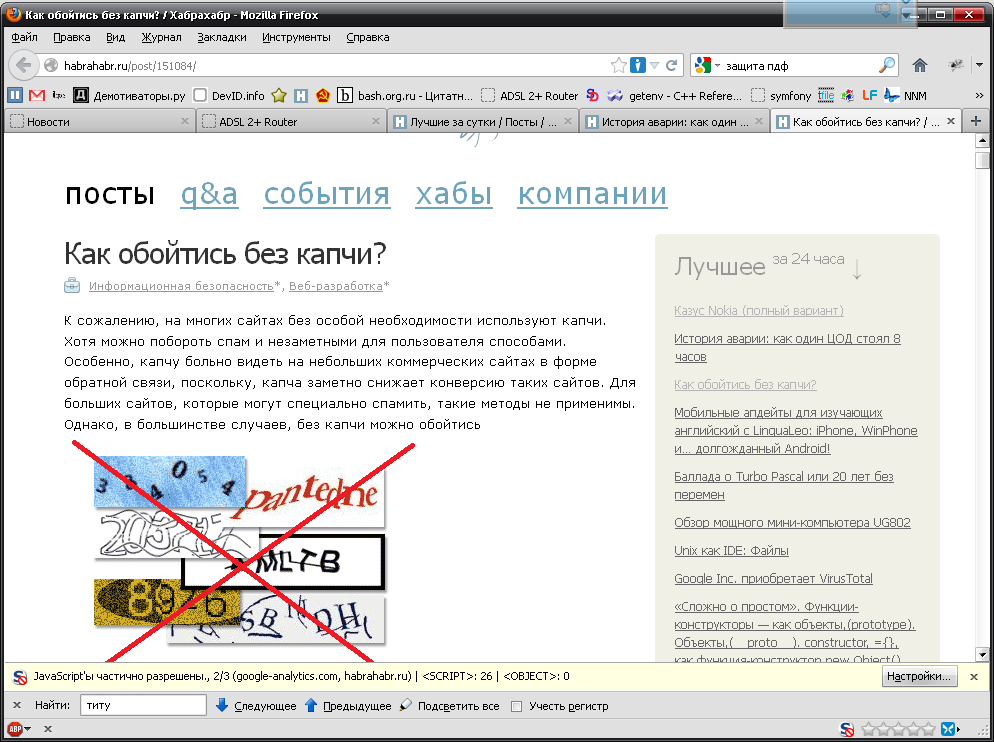
\includegraphics[scale=1,width=10cm]{ap01-09.png}
\caption{Оригінал зображення}
\label{prsc-orig:image}
\end{figure}


\begin{figure}
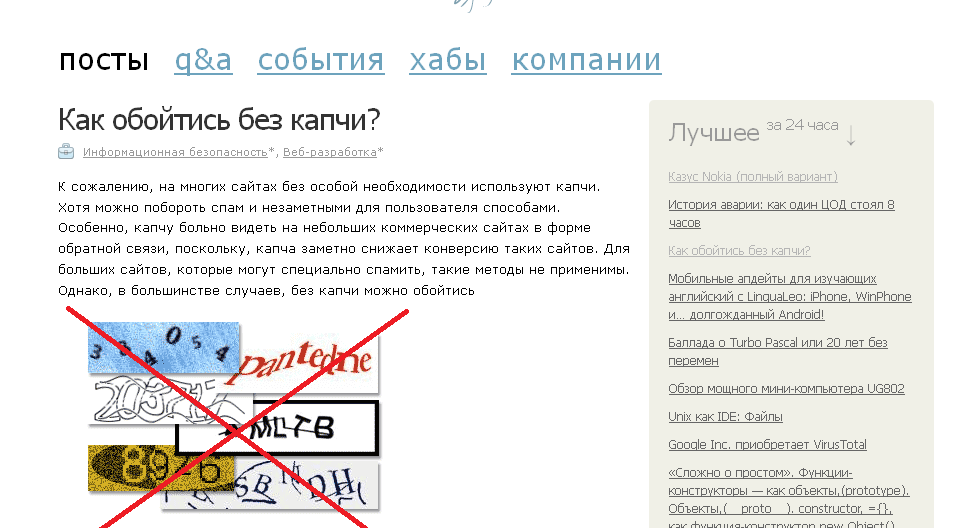
\includegraphics[scale=1,width=10cm]{ap01-10.png}
\caption{Оброблене зображення}
\label{prsc-rel:image}
\end{figure}

\begin{figure}
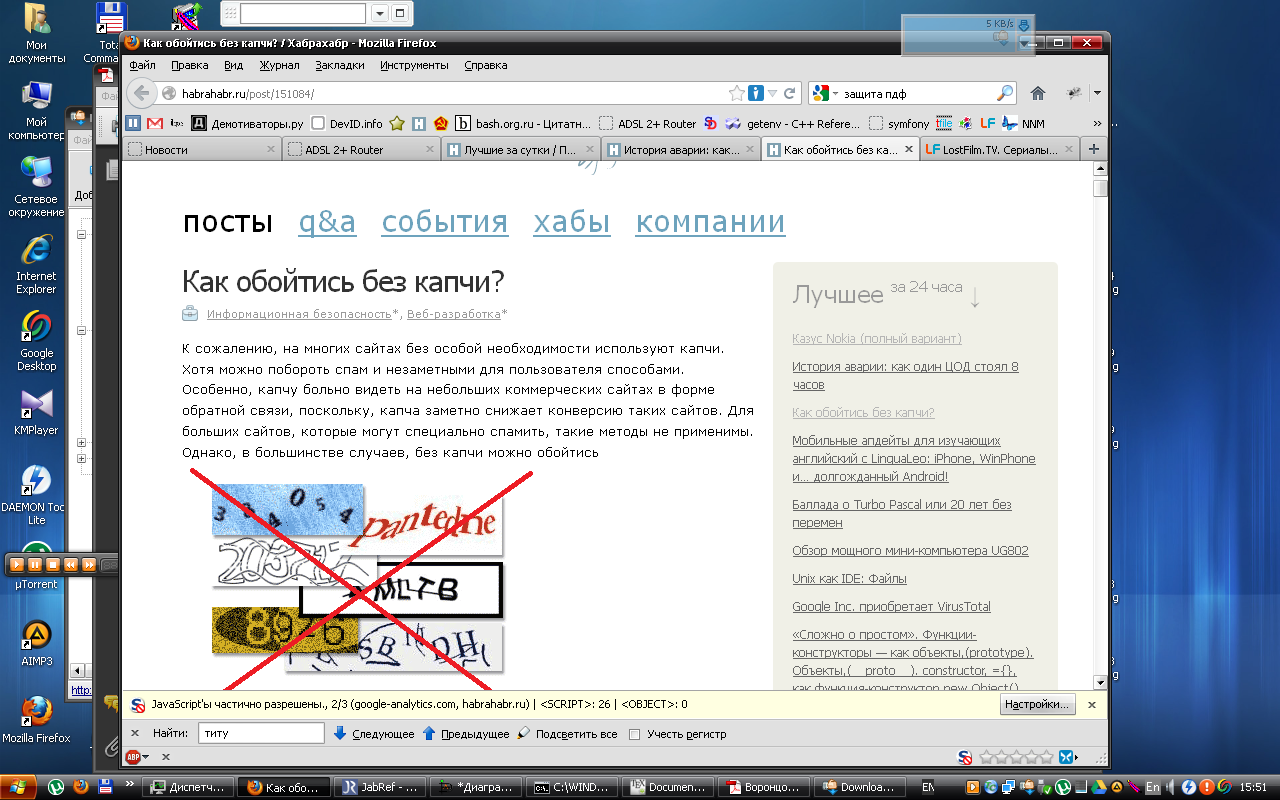
\includegraphics[scale=1,width=10cm]{ap01-11.png}
\caption{Необроблене зображення}
\label{prsc-bad:image}
\end{figure}
\chapter{Матеріали до Л/Р \No 2}
\section{Елементи форм HTML}
\index{HTML!форми}
\subsection{INPUT і його методи}
\index{HTML!форми!input}
\label{inp-tag:app}
\subsection*{Однорядкові поля введення даних}

\begin{verbatim}
<input type=text name=им'я_параметра [value=значення] 
[size=розмір_поля] [maxlen=довжина_поля]>
\end{verbatim}

Даний тег створює поле вводу з максимально допустимою довжиною тексту <<maxlen>> і розміром в size <<знакомест>>. Якщо вказаний атрибут <<value>>, то в поле буде спочатку відображатися значення даного атрибуту. У квадратних дужках \verb'[]' позначені необов'язкові атрибути.

\subsection*{Поля вводу паролів}

\begin{verbatim}
<input type=password name=им'я_параметра [value=значення] 
[size=розмір_поля] [maxlen=довжина_поля]>
\end{verbatim}

Структура даного тегу така сама як і у <input type=text>. Різниця лише у відображенні даних, що вводить користувач.


\subsection*{Приховане текстове поле}

\begin{verbatim}
<input type=hidden name=им'я_параметра [value=значення]>
\end{verbatim}

Такі поля передають дані серверу, але не відображаються на сторінці. Значення атрибуту <<value>> встановлюється при формуванні сторінки, або JavaScript-сценарієм.

\subsection*{Незалежні перемикачі}

\begin{verbatim}
<input type=checkbox name=им'я_параметра [value=значення]
[checked]>
\end{verbatim} 

Перемикач виду <<прапорець>>. У разі встановлення прапорця при відправлені форми серверу будуть передані параметри <<им'я\_параметра=значення>>. Якщо прапорець не встановлено серверу взагалі нічого не буде відправлено. 

Перемикач за замовчуванням вимкнутий, щоб зробити його увімкнутим за замовчуванням треба встановити атрибут  <<checked>>.

Стан перемикача не залежить від стану інших перемикачів цього типу.

\subsection*{Залежні перемикачі}

Залежний перемикач, так само як і незалежний перемикач, може заходитись у двох станах, в залежності від атрибуту  <<checked>>. При цьому на формі може бути увімкнений лише один перемикач серед групи перемикачів з однаковим атрибутом <<name>>.
\begin{verbatim}
<form action="http://localhost/script.php" method="GET">
<input type=radio name=answer value=yes checked>Да
<input type=radio name=answer value=no>Нет
<input type=submit value=Отправить>
</form>
\end{verbatim}

\subsection*{Кнопки відправлення та очищення параметрів форми}

Кнопка відправки служить для передачі серверу змісту форми на сторінці. Атрибут <<value>> визначає текст, ща відображається на кнопці. Під час відправлення форми серверу будуть передані дані кнопки у вигляді <<им'я\_параметра=значення>>.
\begin{verbatim}
<input type=submit [name=им'я_параметра] value=значення>
\end{verbatim}
У разі використання кнопки із зображенням сереру передадуться координати кліку відносно зображення.
\begin{verbatim}
<input type=submit [name=им'я_параметра] src=зображення>
\end{verbatim}
Кнопка очищення форми знищує всі зміни внесені користувачем сайту у дану форму.
\begin{verbatim}
<input type=reset [name=им'я_параметра] value=значення>
\end{verbatim}

\subsection*{Поле вибору файлу}

Тег <input> також дозволяє активувати діалогове вікно вибору файлу та завантажувати його на сервер при відправленні форми.
\begin{verbatim}
<input type=file name=имя [value=имя_файла]>
\end{verbatim}


\subsection{Багаторядкове текстове поле}
\index{HTML!форми!textarea}
\label{tar-tag:app}
Синтаксис багаторядкового поля виглядає наступним чином:
\begin{verbatim}
<textarea name=имя [cols=ширина_в_символах] 
[rows=высота_в_символах] wrap=тип_переноса>
текст за замовчуванням
</textarea>
\end{verbatim}
Хоча висота і ширина поля необов'язкові параметри їх бажано вказувати. Атрибут <<wrap>> відповідає за перенос і може приймати наступні значення:
\begin{enumerate}
\item Virtual --- справа від тексту з'являється полоса прокрутки, а текст розбивається на рядки.
\item Physical --- залежить від браузера і виглядає по-різному
\item None --- текст залишається у тому вигляді, в якому користувач його ввів, з'являються горизонтальна і вертикальна полоси прокрутки.
\end{enumerate}

\subsection{Списки з вибором} \label{sel-tag:app}
\index{HTML!форми!select}
\subsection*{Списки з одиночним вибором}
\label{sel-tag:app}
Списки з одиночним вибором реалізуються за допомогою наступної конструкції:
\begin{verbatim}

<select name=day size=1>
<option value=1>Понедельник</option>
<option value=2>Вторник</option>
<option value=3 selected>Среда</option>
<option value=4>Четверг</option>
<option value=5>Пятница</option>
<option value=6>Суббота</option>
<option value=7>Воскресенье</option>
</select>

\end{verbatim}
При відправленні форми сервер отримає дані виду <<им'я\_параметра=значення>>. За замовчуванням може бути обраний пункт списку серед атрибутів якого є \verb'selected'.

\subsection*{Списки з множинним вибором}
Список з множинним вибором відрізняється лише атрибутом \verb'multiple' в середині тега \verb'<select>'.
\begin{verbatim}

<select name=day size=7 multiple>
<option value=1>Понедельник</option>
<option value=1>Вторник</option>
<option value=1>Среда</option>
<option value=1>Четверг</option>
<option value=1>Пятница</option>
<option value=1>Суббота</option>
<option value=1>Воскресенье</option>
</select>


\end{verbatim}


\section{Змінні-функції}
\index{PHP!функції!змінні-функції}
\label{var-func:app}
Приклад використання змінної-функції:
\begin{verbatim}
<?php
?php
function foo() {
    echo "In foo()<br />\n";
}
function bar($arg = '')
{
    echo "In bar(); argument was '$arg'.<br />\n";
}
// Функция-обертка для echo
function echoit($string)
{
    echo $string;
}

$func = 'foo';
$func();        // Вызывает функцию foo()
$func = 'bar';
$func('test');  // Вызывает функцию bar()
$func = 'echoit';
$func('test');  // Вызывает функцию echoit()
\end{verbatim}
\chapter{Матеріали до Л/Р \No 3}

\section{Змінні оточення web-сервера Apache}
\label{var-apa:app}
\nopagebreak[4]
\index{Web-сервери!Apache!змінні оточення}
\subsection{Формовані сервером змінні}

\textbf{AUTH\_TYPE} Використовується схема аутентифікації. Зазвичай BASIC

\textbf{CONTENT\_LENGTH} Довжина вмісту

\textbf{CONTENT\_TYPE} MIME-тип вмісту

\textbf{GETAWAY\_INTERFACE} Версія CGI, наприклад CGI/1.1

\textbf{PATH\_info} HTTP-шлях до сценарію

\textbf{PATH\_TRANSLATED} Повний шлях до сценарію

\textbf{REMOTE\_ADDR} IP-адреса запитуваного комп'ютера-клієнта

\textbf{REMOTE\_HOST} Доменне ім'я запитувача комп'ютера (якщо доступно). Доменне ім'я визначається веб-сервером за допомогою служби DNS. Директива \verb'HostnameLookups' сервера Apache дозволяє (або забороняє) перетворення IP-адреси в доменне ім'я.

\textbf{REMOTE\_PORT} Порт, закріплений за браузером для отримання відповіді від сервера

\textbf{REMOTE\_USER} Ім'я користувача, що пройшов аутентифікацію

\textbf{QUERY\_STRING} Рядок переданих серверу параметрів

\textbf{SERVER\_ADDR} IP-адресу сервера

\textbf{SERVER\_NAME} Доменне ім'я сервера. Визначається директивою ServerName файлу конфігурації

\textbf{SERVER\_PORT} TCP-порт Web-сервера. Зазвичай 80

\textbf{SERVER\_PROTOCOL} Версія протоколу HTTP. Наприклад, HTTP/1.1

\textbf{SERVER\_SOFTWARE} Програмне забезпечення сервера

\textbf{SCRIPT\_NAME} HTTP-шлях до сценарію

\textbf{SCRIPT\_FILENAME} Файл сценарію в файловій системі сервера (фізичний шлях). Наприклад, \verb'/var/www/cgi-bin/script.cgi'


\subsection{Спеціальні змінні сервера Apache}

\textbf{DOCUMENT\_ROOT} Фізичний шлях до кореневого WWW-каталогу сервера. Наприклад, \verb'/var/www.html/'

\textbf{SERVER\_ADMIN} Адреса електронної пошти адміністратора сервера

\textbf{SERVER\_SIGNATURE} Підпис сервера. Наприклад, <<\verb'Apache/1.3.3 сервера на www.somefirm.com порт 80'>>


\subsection{Змінні HTTP-полів запиту}

\textbf{HTTP\_HOST} Ім'я віртуального хоста, якому адресовано запит

\textbf{HTTP\_USER\_AGENT} Програмне забезпечення віддаленого користувача. Зазвичай ця змінна оточення містить назву і версію браузера

\textbf{HTTP\_ACCEPT} Список підтримуваних клієнтом типів інформації. 

\textbf{HTTP\_ACCEPT\_LANGUAGE} Список підтримуваних мов в порядку переваги, наприклад, RU, EN

\textbf{HTTP\_ACCEPT\_ENCODING} Список підтримуваних методів стиснення

\textbf{HTTP\_ACCEPT\_CHARSET} Список підтримуваних кодувань

\textbf{HTTP\_CONNECTION} Тип з'єднання. Можливі два варіанти:
\begin{list}{•}{•}
\item \verb'Keep-Alive'~--- якщо після відповіді на запит не потрібно розривати з'єднання;
\item \verb'Close'~--- якщо потрібно закрити з'єднання відразу після відповіді на запит.
\end{list}

\textbf{HTTP\_REFERER} Значення поля \verb'REFERER'. У цьому полі браузер передає URL ресурсу, який посилається на наш сервер. Наприклад, якщо користувач перейшов на сайт зі сторінки http://www.somehost.com/page.php, то значення поля \verb'REFERER' буде http://www.somehost.com/page.php.

\textbf{HTTP\_X\_FORWARDED\_FOR} Якщо користувач працює через проксі-сервер, то в цьому полі буде IP-адреса комп'ютера, який звернувся до проксі-сервера. Якщо це поле вже містить значення, то нове значення буде додано через кому.



\subsection{Суперглобальні масиви PHP}
\index{PHP!змінні!суперглобальні масиви}
\label{sup-glob:app}

\textbf{\$GLOBALS}~--- масив всіх глобальних змінних (у тому числі і для користувача).

\textbf{\$\_SERVER}~--- містить безліч інформації про поточний запит і сервер.

\textbf{\$\_ENV}~--- поточні змінні середовища. Їх набір специфічний для кожної конкретної платформи, на якій виконується сценарій.

\textbf{\$\_GET}~--- асоціативний масив з параметрами GET-запиту. У початковому вигляді ці параметри доступні в \verb|$_SERVER ['QUERY\_STRING']| і в \verb|$_SERVER ['REQUEST_URI']| в складі URI.

\textbf{\$\_POST}~--- асоціативний масив значень полів HTML-форми при відправки методом POST.

\textbf{\$\_FILES}~--- асоціативний масив з відомостями про надіслані методом POST файлах. Кожен елемент має індекс ідентичний значенню атрибута \verb'name' у формі і, в свою чергу, також є масивом з наступними елементами:
\begin{enumerate}
\item \verb|$_FILES['name']|~--- вихідне ім'я файлу на комп'ютері користувача.
\item \verb|$_FILES['type']|~--- зазначений агентом користувача MIME~--- тип файлу.
\item \verb|$_FILES['size']|~--- розмір файлу в байтах.
\item \verb|$_FILES['tmp_name']|~--- повний шлях до файлу в тимчасовій папці.
\item \verb|$_FILES['error']|~--- код помилки.
\end{enumerate}

\textbf{\$\_COOKIE}~--- асоціативний масив з переданими агентом користувача значеннями cookie.

\textbf{\$\_REQUEST}~--- загальний масив ввідних даних запиту користувача як в масивах \verb'$_GET, $_POST, $_COOKIE'. Починаючи з версії PHP 4.1 включається і вміст \verb'$_FILES'.


\section{Пріоритети виконання операторів}
\index{PHP!оператори!пріоритети}


\begin{center}
\begin{longtable}[t]{|c|p{25em}|}
\caption{Пріоритети виконання операторів} \label{pr-op:table}\\
\hline

Асоціативність & Оператор \\
\hline \endfirsthead
\caption*{\space Продовження} \\
\hline
Асоціативність & Оператор \\
\hline \endhead
\hline \endfoot
неасоціативна	& \verb|new| \\
права	& \verb|[|\\
неасоціативна	& \verb|++ --| \\
неасоціативна	& \verb|! ~ -(int) (float) (string) (array) (object) @| \\
ліва	& \verb|* / %| \\
ліва	& \verb|+ - .| \\
ліва	& \verb|<< >>| \\
неассоціативна	& \verb|< <= > >=| \\
неассоціативна	& \verb|== != === !==| \\
ліва	& \verb|&| \\
ліва	& \verb|^| \\
ліва	& \verb'|' \\
ліва	& \verb|&&| \\
ліва	& \verb'||' \\
ліва	& \verb|? :| \\
права	& \verb'= += -= *= /= .= %= &= |= ^= <<= >>='  \\
\penalty -10000
ліва	& \verb|and| \\
ліва	& \verb|xor| \\
ліва	& \verb|or| \\
ліва	& \verb|,| \\

\hline
\end{longtable}
\end{center}
\chapter{Матеріали до Л/Р \No 4}

\section{Рядки та регулярні вирази}
\subsection{Функції роботи з рядками}
\label{str-func:app}
\nopagebreak[4]


\index{PHP!змінні!рядки!функції}
\begin{longtable}[t]{|l|p{21em}|}

\caption{\space Повний список функцій роботи з рядками} \label{str-func:table}\\
\hline

Функція & Опис \\
\hline \endfirsthead
\caption*{\space Продовження} \\
\hline
Функція & Опис \\
\hline \endhead
\hline \endfoot
addcslashes & екрануючі спецсимволи в стилі мови C \\
addslashes & екрануючі спецсимволи в рядку \\
bin2hex & Перетворює бінарні дані у шістнадцятірічне подання \\
chr & Повертає символ за його кодом \\
chunk\_split & Розбиває рядок на фрагменти \\
convert\_cyr\_string & Перетворює рядок з одного кириличної кодування в інше \\
count\_chars & Повертає інформацію про символи, що входять в рядок \\
crc32 & Обчислює CRC32 для рядка \\
crypt & Необоротне шифрування (хешування) \\
echo & Виводить одну чи більше рядків \\
explode & Розбиває рядок на підрядки \\
fprintf & Записує отформатированную рядок у потік \\
get\_html\_translation\_table & Повертає таблицю перетворень \\
hebrev & Перетворює текст на івриті з логічного кодування у візуальне \\
hebrevc & Перетворює текст на івриті з логічнго кодування у візуальне з перетворенням в переклад \\
htmlentities & Перетворює символи у відповідні HTML теги \\
htmlspecialchars & Перетворює спеціальні символи в HTML теги \\
html\_entity\_decode & Перетворює HTML теги в відповідні символи \\
implode & Об'єднує елементи масиву в рядок \\
localeconv & Повертає інформацію про числові формати \\
ltrim & Видаляє пробіли з початку рядка \\
md5 & Повертає MD5-хеш рядка \\
md5\_file & Повертає MD5-хеш файлу \\
metaphone & Повертає ключ metaphone для рядка \\
nl2br & Вставляє HTML-код розриву рядка перед кожним переведенням рядка \\
number\_format & Форматує число з поділом груп \\
ord & Повертає ASCII-код символу \\
parse\_str & Розбирає рядок у змінні \\
print & Виводить рядок \\
printf & Виводить відформатований рядок \\
quoted\_printable\_decode & розкодує рядок, закодовану методом quoted printable \\
quotemeta & екрануючі спеціальні символи \\
rtrim & Видаляє пробіли з кінця рядка \\
sha1 & Повертає SHA1-хеш рядка \\
sha1\_file & Повертає SHA1-хеш файлу \\
similar\_text & Обчислює ступінь схожості двох рядків \\
soundex & Повертає ключ soundex для рядка \\
sprintf & Повертає відформатований рядок \\
sscanf & Розбирає рядок у відповідності із заданим форматом \\
strcasecmp & Порівняння рядків без урахування регістра, безпечне для даних у двійковій формі \\
strcmp & Порівняння рядків, безпечне для даних у двійковій формі \\
strcoll & Порівняння рядків з урахуванням поточної локалі \\
strcspn & Повертає довжину ділянки на початку рядка, не відповідного  масці \\
stripcslashes & Видаляє екранування символів, вироблене функцією addcslashes () \\
stripos & Повертає позицію першого входження підрядка без урахування регістра \\
stripslashes & Видаляє екранування символів, вироблене функцією addslashes () \\
strip\_tags & Видаляє HTML і PHP теги з рядка \\
stristr & Аналог функції strstr, але незалежний від регістру \\
strlen & Повертає довжину рядка \\
strnatcasecmp & Порівняння рядків без урахування регістра з використанням алгоритму \\
strnatcmp & Порівняння рядків з використанням алгоритму "природнього упорядкування" \\
strncasecmp & порівняння перших n символів рядків без урахування регістра, безпечне для даних у двійковій формі \\
strncmp & порівняння перших n символів рядків без урахування регістра, безпечне для даних у двійковій формі \\
strpos & Знаходить перше входження підрядка в рядок \\
strrchr & Знаходить останнє входження символу в рядок \\
strrev & Перевертає рядок \\
strripos & Повертає позицію останнього входження підрядка без урахування регістра \\
strrpos & Знаходить останнє входження символу в рядок \\
strspn & Повертає довжину ділянки на початку рядка, відповідного масці \\
strstr & Знаходить перше входження підрядка \\
strtok & Розбиває рядок \\
strtolower & Перетворює рядок у нижній регістр \\
strtoupper & Перетворює рядок у верхній регістр \\
strtr & Перетворює задані символи \\
str\_ireplace & Регістро-незалежний варіант функції str\_replace (). \\
str\_pad & Доповнює рядок інший рядком до заданої довжини \\
str\_repeat & Повертає повторювану рядок \\
str\_replace & Замінює рядок пошуку на рядок заміни \\
str\_rot13 & Виконує над рядком перетворення ROT13 \\
str\_shuffle & перемішує символи в рядку \\
str\_split & Розбиває рядок в масив \\
str\_word\_count & Повертає інформацію про слова, що входять в рядок \\
substr & Функція повертає частину рядка \\
substr\_count & Підраховує кількість входжень підрядка в рядок \\
substr\_replace & Замінює частину рядка \\
trim & Видаляє пробіли з початку та кінця рядка \\
ucfirst & Перетворює перший символ рядка в верхній регістр \\
ucwords & Перетворює у верхній регістр перший символ кожного слова в рядку \\
vprintf & Виводить відформатований рядок \\
vsprintf & Повертає відформатований рядок \\
wordwrap & Виконує перенесення рядка на дану кількість символів з використанням символу розриву рядка \\
\hline
\end{longtable}

\subsection{Метасимволи та керуючі конструкцію регулярних виразів у MySQL}
\label{chr-rxp:app}
\index{PHP!регулярні вирази}
У додатку надано перелік метасимволів та керуючих конструкцій для регулярних виразів, що підтримуються у СУБД MySQL.  

\pagebreak[4]
\begin{longtable}[t]{|l|p{20em}|}
\caption{Спецпослідовності регулярних виразів POSIX 1003.2 для MySQL} \label{chr2-rxp:table}\\
\hline

Позначення & Опис \\
\hline

\verb'\t' & символ табуляции. \\
\verb'\f' & конец файла. \\
\verb'\n' & символ перевода строки. \\
\verb'\r' & символ возврата каретки. \\
\verb'\\' & символ обратного слэша \verb'\'. \\


\hline
\end{longtable}


\pagebreak[3]

\begin{longtable}[t]{|l|p{20em}|}

\caption{Опис метасимволів регулярних виразів POSIX 1003.2 для MySQL} \label{chr-rxp:table}\\
\hline

Позначення & Опис \\
\hline




\verb|^| & Відповідає початку рядка. \\

\verb|$| & Відповідає кінцю рядка. \\

\verb|.| & Відповідає будь-якому символу. \\

\verb|a*| & Відповідає будь-якій послідовності з 0 або більше символів <<a>>. \\

\verb|a+| & Відповідає будь-якій послідовності з 1 або більше символів <<a>>. \\

\verb|a?| & Відповідає 0 або 1 символу <<a>>. \\

\verb'de|abc' & Відповідає послідовності <<de>> або <<abc>>. \\

\verb|(abc)*| & Відповідає 0 або більше послідовностям <<abc>>.  \\

\verb|[a-dX],[^a-dX]| & Відповідає будь-якому символу, який є (або не яв ляется, якщо використовується \verb|^|) будь-яким із символів а, Ь, с, d або X. Символ '-' між двома іншими символами утворює інтервал. \\
  
\hline
\end{longtable}


\pagebreak[3]



\begin{longtable}[t]{|l|p{20em}|}

\caption{Класи символів регулярних виразів POSIX 1003.2 для MySQL} \label{chr3-rxp:table}\\
\hline

Позначення & Опис \\
\hline


\verb|[:alnum:]| & алфавітно цифрові символи. \\
\verb|[:alpha:]| & символи алфавіту. \\
\verb|[:blank:]| & символи пробілу і табуляції. \\
\verb|[:cntrl:]| & керуючі символи. \\
\verb|[:digit:]| & десяткові цифри (0-9). \\
\verb|[:graph:]| & графічні (видимі) символи. \\
\verb|[:lower:]| & символи алфавіту в нижньому регістрі. \\
\verb|[:print:]| & графічні або невидимі символи. \\
\verb|[:punct:]| & знаки пунктуації. \\
\verb|[:space:]| & символи пробілу, табуляції, нового рядка або повернення каретки. \\
\verb|[:upper:]| & символи алфавіту в верхньому регістрі. \\
\verb|[:xdigit:]| & шістнадцяткові цифри. \\

\hline
\end{longtable}


\pagebreak[3]




\chapter{Матеріали до Л/Р \No 5}



\section{Функції для роботи з файловою системою}
\index{Файл!функції}
\begin{longtable}[t]{|l|p{20em}|}
\kill
\caption{\space Перелік функцій для роботи з ФС} \label{fs-funcr:table}\\
\hline

функція & Опис \\
\hline \endfirsthead
\caption*{\space Продовження} \\
\hline
функція & Опис \\
\hline \endhead
\hline \endfoot



\verb'basename' & Повертає останній компонент імені з вказаного шляху\\
\verb'chgrp' & Змінює групу власників файлу\\
\verb'chmod' & Змінює режим доступу до файлу\\
\verb'chown' & Змінює власника файлу\\
\verb'clearstatcache' & Очищає кеш стану файлів\\
\verb'copy' & Копіює файл\\
\verb'delete' & См.опис функції unlink або unset\\
\verb'dirname' & Повертає ім'я батьківського каталогу з зазначеного шляху\\
\verb'disk_free_space' & Повертає розмір доступного простору в каталозі або в файловій системі\\
\verb'disk_total_space' & Повертає загальний розмір каталогу або розділу файлової системи\\
\verb'diskfreespace' & Псевдонім disk\_free\_space\\
\verb'fclose' & Закриває відкритий дескриптор файлу\\
\verb'feof' & Перевіряє, чи досягнутий кінець файлу\\
\verb'fflush' & Скидає буфер виводу у файл\\
\verb'fgetc' & Зчитує символ з файлу\\
\verb'fgetcsv' & Читає рядок з файлу і виробляє розбір даних CSV\\
\verb'fgets' & Читає рядок з файлу\\
\verb'fgetss' & Читає рядок з файлу і відкидає HTML-теги\\
\verb'file_exists' & Перевіряє наявність вказаного файлу або каталогу\\
\verb'file_get_contents' & Читає вміст файлу в рядок\\
\verb'file_put_contents' & Пише рядок в файл\\
\verb'file' & Читає вміст файлу і поміщає його в масив\\
\verb'fileatime' & Повертає час останнього доступу до файлу\\
\verb'filectime' & Повертає час зміни індексного дескриптора файлу\\
\verb'filegroup' & Отримує ідентифікатор групи файлу\\
\verb'fileinode' & Повертає індексний дескриптор файлу\\
\verb'filemtime' & Повертає час останньої зміни файлу\\
\verb'fileowner' & Повертає ідентифікатор власника файлу\\
\verb'fileperms' & Повертає інформацію про права на файл\\
\verb'filesize' & Повертає розмір файлу\\
\verb'filetype' & Повертає тип файлу\\
\verb'flock' & Переносима консультативна блокування файлів\\
\verb'fnmatch' & Перевіряє збіг імені файлу з шаблоном\\
\verb'fopen' & Відкриває файл або URL\\
\verb'fpassthru' & Виводить всі залишилися дані з файлового покажчика\\
\verb'fputcsv' & Форматує рядок у вигляді CSV і записує його в файловий покажчик\\
\verb'fputs' & Псевдонім fwrite\\
\verb'fread' & бінарних-безпечне читання файлу\\
\verb'fscanf' & Обробляє дані з файлу відповідно до формату\\
\verb'fseek' & Встановлює зсув у файловому покажчику\\
\verb'fstat' & Отримує інформацію про фото використовуючи відкритий файловий покажчик\\
\verb'ftell' & Повідомляє поточну позицію читання/запису файлу\\
\verb'ftruncate' & Врізає файл до вказаної довжини\\
\verb'fwrite' & бінарно-безпечний запис в файл\\
\verb'glob' & Знаходить файлові шляху, що збігаються з шаблоном\\
\verb'is_dir' & Визначає, чи є ім'я файлу директорією\\
\verb'is_executable' & Визначає, чи є файл виконуваним\\
\verb'is_file' & Визначає, чи є файл звичайним файлом\\
\verb'is_link' & Визначає, чи є файл символічним посиланням\\
\verb'is_readable' & Визначає наявність файлу і доступний він для читання\\
\verb'is_uploaded_file' & Визначає, чи був файл завантажений за допомогою HTTP POST\\
\verb'is_writable' & Визначає, чи доступний файл для запису\\
\verb'is_writeable' & Псевдонім is\_writable\\
\verb'lchgrp' & Змінює групу, якій належить символічне посилання\\
\verb'lchown' & Змінює власника символічного посилання\\
\verb'link' & Створює жорстке посилання\\
\verb'linkinfo' & Повертає інформацію про посиланню\\
\verb'lstat' & Повертає інформацію про фото або символічної посиланню\\
\verb'mkdir' & Створює директорію\\
\verb'move_uploaded_file' & Переміщає завантажений файл у нове місце\\
\verb'parse_ini_file' & Обробляє конфігураційний файл\\
\verb'parse_ini_string' & Розбирає рядок конфігурації\\
\verb'pathinfo' & Повертає інформацію про шлях до файлу\\
\verb'pclose' & Закриває файловий покажчик процесу\\
\verb'popen' & Відкриває файловий покажчик процесу\\
\verb'readfile' & Виводить файл\\
\verb'readlink' & Повертає файл, на який вказує символьне посилання\\
\verb'realpath_cache_get' & Отримує записи з кешу реального шляху\\
\verb'realpath_cache_size' & Отримує розмір кеша реального шляху\\
\verb'realpath' & Повертає канонізований абсолютний шлях до файлу\\
\verb'rename' & Перейменовує файл або директорію\\
\verb'rewind' & Скидає курсор у файлового покажчика\\
\verb'rmdir' & Видаляє директорію\\
\verb'set_file_buffer' & Псевдонім stream\_set\_write\_buffer\\
\verb'stat' & Повертає інформацію про файл\\
\verb'symlink' & Створює символічну посилання\\
\verb'tempnam' & Створює файл з унікальним ім'ям\\
\verb'tmpfile' & Створює тимчасовий файл\\
\verb'touch' & Встановлює час доступу і модифікації файлу\\
\verb'umask' & Змінює поточну umask\\
\verb'unlink' & Видаляє файл \\


\hline
\end{longtable}



\section{Параметри функції <<fopen()>>}
\begin{longtable}[t]{|c|p{27em}|}
\kill
\caption{\space Другий параметр функції <<fopen()>>} \label{fo-par:table}\\
\hline

Параметр & Опис \\
\hline \endfirsthead
\caption*{\space Продовження} \\
\hline
Параметр & Опис \\
\hline \endhead
\hline \endfoot
\verb'R' & Відкриває файл тільки для читання; поміщає покажчик в початок файлу. \\ \hline
\verb'R+' & Відкриває файл для читання і запису; поміщає покажчик в початок файлу. \\ \hline
\verb'W' & Відкриває файл тільки для запису; поміщає покажчик в початок файлу і обрізає файл до нульової довжини. Якщо файл не існує~--- намагається його створити. \\ \hline
\verb'W+' & Відкриває файл для читання і запису; поміщає покажчик в початок файлу і обрізає файл до нульової довжини. Якщо файл не існує~--- намагається його створити. \\ \hline
\verb'A' & Відкриває файл тільки для запису; поміщає покажчик в кінець файлу. Якщо файл не існує~--- намагається його створити. \\ \hline
\verb'A+' & Відкриває файл для читання і запису; поміщає покажчик в кінець файлу. Якщо файл не існує~--- намагається його створити. \\ \hline
\verb'X' & Створює і відкриває тільки для запису; поміщає покажчик в початок файлу. Якщо файл вже існує, виклик \verb'fopen()' закінчиться невдачею, поверне \verb'FALSE' і видасть помилку \verb'E_WARNING'. Якщо файл не існує, спробує його створити. \\ \hline
\verb'X+' & Створює і відкриває для читання і запису інакше поверне \verb'FALSE'. \\ \hline
\verb'C' & Відкриває файл тільки для запису. Якщо файл не існує, то він створюється. Якщо ж файл існує, то він не обрізається, і виклик цієї функції не викликає помилку. Покажчик на файл буде встановлений на початок файлу.\\ \hline
\verb'C+' & Відкриває файл для читання і запису інакше функція має ту ж поведінку, що і з використанням <<\verb'c'>>. \\ \hline

\hline
\end{longtable}


\section{Функції для роботи з каталогами}
\index{Каталог!функції}
\begin{longtable}[t]{|c|p{27em}|}
\kill
\caption{\space Перелік функцій для роботи з каталогами} \label{dir-func:table}\\
\hline

Функція & Опис \\
\hline \endfirsthead
\caption*{\space Продовження} \\
\hline
Функція & Опис \\
\hline \endhead
\hline \endfoot
\verb'chdir' & Змінює каталог\\
\verb'mkdir' & Створює каталог\\
\verb'rmdir' & Видаляє каталог\\
\verb'is_dir' & Перевіряє чи є об'єкт каталогом\\
\verb'chroot' & Змінює кореневий каталог\\
\verb'closedir' & Звільняє дескриптор каталогу\\
\verb'dir' & Повертає екземпляр класу Directory\\
\verb'getcwd' & Отримує ім'я поточного робочого каталога\\
\verb'opendir' & Відкриває дескриптор каталогу\\
\verb'readdir' & Отримує елемент каталогу за його дескриптору\\
\verb'rewinddir' & Скинути дескриптор каталогу\\
\verb'scandir' & Отримує список файлів і каталогів, розташованих по зазначеному шляху \\

\hline
\end{longtable}

\chapter{Матеріали до Л/Р \No 6}


\section{Налаштування сесії у РНР}
\index{Сесії!налаштування}
\begin{longtable}[t]{|l|p{20em}|}
\kill
\caption{\space Перелік параметрів у файлі php.ini} \label{ses-opt:table}\\
\hline

Опція & Опис \\
\hline \endfirsthead
\caption*{\space Продовження} \\
\hline
Опція & Опис \\
\hline \endhead
\hline \endfoot

\verb'session.save_path' & визначає, де на сервері зберігатимуться дані сесії. \\
\verb'session.use_cookies' & визначає, чи використовувати cookies при роботі з сесіями.\\
\verb'session.cookie_lifetime' & задає тривалість життя cookies в секундах.\\
\verb'session.name' & визначає ім'я сесії\\
\verb'session.auto_start' & дозволяє автоматично запускати сесії\\
\verb'session.serialize_handler' & задає спосіб кодування даних сесії\\
\verb'session.cache_expire' & визначає, через скільки хвилин застаріває документ в кеші\\

\hline
\end{longtable}

Ім'я сесії \verb'session.name' за умовчанням встановлюється як \verb'PHPSESSID' і використовується в \verb'cookies' як ім'я змінної, в якій зберігається ідентифікатор сесії. Автоматичний запуск сесій за замовчуванням відключений, але його можна задати, зробивши значення \verb'session.auto_start' рівним <<1>>. Для кодування даних сесії по замовчуванню використовується php. Старіння даних, збережених в кеші, відбувається через 180 хвилин.

\section{Повний перелік змінних у <<php.ini>>}
\begin{longtable}[t]{|l|p{15em}|}
\kill

\caption{\space Повний параметрів у файлі <<php.ini>> та значень за замовчуванням} \label{ses-opt-full:table}\\
\hline

Опція & Значення \\
\hline \endfirsthead
\caption*{\space Продовження} \\
\hline
Опція & Значення \\
\hline \endhead
\hline \endfoot

\verb'session.save_path' & \verb'""'\\
\verb'session.name' & "PHPSESSID"\\
\verb'session.save_handler' & "files"\\
\verb'session.auto_start' & "0"\\
\verb'session.gc_probability' & "1"\\
\verb'session.gc_divisor' & "100"\\
\verb'session.gc_maxlifetime' & "1440"\\
\verb'session.serialize_handler' & "php"\\
\verb'session.cookie_lifetime' & "0"\\
\verb'session.cookie_path' & "/"\\
\verb'session.cookie_domain' & \verb'""'\\
\verb'session.cookie_secure' & \verb'""'\\
\verb'session.cookie_httponly' & \verb'""'\\
\verb'session.use_cookies' & "1"\\
\verb'session.use_only_cookies' & "1"\\
\verb'session.referer_check' & \verb'""'\\
\verb'session.entropy_file' & \verb'""'\\
\verb'session.entropy_length' & "0"\\
\verb'session.cache_limiter' & "nocache"\\
\verb'session.cache_expire' & "180"\\
\verb'session.use_trans_sid' & "0"\\
\verb'session.bug_compat_42' & "1"\\
\verb'session.bug_compat_warn' & "1"\\
\verb'session.hash_function' & "0"\\
\verb'session.hash_bits_per_character' & "4"\\
\verb'url_rewriter.tags' & "a=href, area=href, frame=src, form=, fieldset="\\
\verb'session.upload_progress.enabled' & "1"\\
\verb'session.upload_progress.cleanup' & "1"\\
\verb'session.upload_progress.prefix' & "upload\_progress\_"\\
\verb'session.upload_progress.name' & "PHP\_SESSION\_ UPLOAD\_PROGRESS"\\
\verb'session.upload_progress.freq' & "1\%"\\
\verb'session.upload_progress.min_freq' & "1"\\


\hline
\end{longtable}


\section{Опис функцій для роботи з сесіями}
\index{PHP!функції!сесії}
\label{ses-func:text}
Нижче дано перелік функцій, що необхідні для роботи із сесіями. Деякі функції налаштування дублюють функціонал опцій у файлі <<php.ini>>, на такі функції буде звернено увагу.

\textbf{session\_destroy()}

Функція скасовує дію \verb'session_start()'. Викликати потрібно після виклику \verb'session_start()'. Можна застосовувати, щоб знищувати сессіію користувача, а потім відразу викликати в програмі вдруге \verb'session_start()', вийти зовсім новий відвідувач з новим ідентифікатором і чистої сесією.

\textbf{session\_name()} або \verb'session.name'

РНР для зберігання ідентифікатора використовує якусь змінну. В cookies записують змінну: значення змінної~--- ідентифікатор, назва змінної~--- PHPSESSID. PHPSESSID~--- це назва, яку використовують за замовчуванням. Її можна перейменувати у щось більш коротке, наприклад SID. А для цього треба замінити параметр \verb'session.name' на значення SID: 

можна замінити php.ini: \verb'session.name = SID' 

можна створити. htaccess файл у каталозі з скриптами вашого сайту і помістити рядок \verb'php_value session.name SID'

Щоб отримати назву змінної, яку використовують для зберігання ідентифікатора, треба скористатися функцією без параметра \$name = \verb'session_name()'.

Щоб встановити таку змінну в довільну назву, скористайтеся функцією з параметром \verb'session_name("МояНазва")'. Зрозуміло, якщо Вам чомусь знадобилося змінити ім'я змінної для cookies за допомогою цієї функції, то її треба викликати перед \verb'session_start()' або \verb'session_register()'.

\textbf{session\_module\_name()} або \verb'session_save_handler'

Отримати або встановити поточний модуль сесії. РНР може зберігати сесії різному вигляді. За замовчуванням~--- в файлах.

\textbf{session\_save\_path()} або \verb'session.save_path'

Отримати або встановити каталог, в якому будуть зберігатися файли сесії. \$path = \verb'session_save_path()'~--- отримати. \verb'session_save_path("/mydir/temp")'~--- встановити. Параметр \verb'session.save_path' можна задавати в php.ini або <<.htaccess>>. 

\textbf{session\_id()}

Отримати або встановити ідентифікатор відвідувача (128-бітове число, представлене у вигляді рядка в 32 байти). У нормальних умовах Вам не потрібно встановлювати номер сесії. Але якщо Ви хочете для всіх своїх відвідувачів використовувати одну сессіію, то перед \verb'session_start()' придумайте будь-яке ім'я (наприклад, \verb'session_id ("my_name")') або отримаєте справжній ідентифікатор іншим чином. Виклик функції без параметрів поверне Вам поточний номер сесії (в такому випадку~--- викликати після \verb'session_start()').

\textbf{session\_register()}

Зареєструвати одну або кілька змінних. Передавати треба імена змінних, а не їх значення: \verb'session_register("змінна1", "змінна2", ...)'. 

\textbf{session\_unregister()}

Видалити з сесії необхідну змінну. Можна передати тільки одне ім'я змінної за один виклик функції.

\textbf{session\_unset()}

Очистити всі змінні сесії. У відмінності від \verb'session_destroy()' сесія і ідентифікатор залишається.

\textbf{session\_is\_registered()}

Перевірити, зареєстрована якась змінна в поточній сесії чи ні:

\verb'if (session_is_registered("змінна")) ...'

\textbf{session\_get\_cookies\_params()} і

\textbf{session\_set\_cookies\_params()}

Отримати інформацію про cookies, що зберігає змінну з ідентифікатором сесії, можна наступним чином:

\begin{verbatim}
echo "<pre> session INFO: \ n";
print_r (session_get_cookies_params());
\end{verbatim}

Так можна дізнатися про час життя змінної, домен та шляхи cookies.

Функцією \verb'session_set_cookies_params()' можна перевстановити параметри (хоча всі ці параметри задані в php.ini).

\textbf{session\_decode()} і \textbf{session\_encode()}

Декодування закодованих рядків у сесії і кодування змінних у рядок сесії.

\textbf{session\_set\_save\_handler()}

Можливо, Вас не влаштовують варіанти зберігання сесій, що пропонуються в РНР. Може бути, ви хочете зберігати сесії в простих текстових файлах, щоб їх можна було легко редагувати. Тоді Вам потрібно створити декілька функцій, що відповідають за функціонування сесій і передати назви цих функцій в \verb'session_set_save_handler()'.

\chapter{Матеріали до Л/Р \No 7}
\section{Синтаксис команди CREATE TABLE}
\index{MySQL!SQL!CREATE}
\label{crtab:text}
\begin{verbatim}
 CREATE [TEMPORARY] TABLE [IF NOT EXISTS] 
 tbl_name [(create_definition, ...)]
 [Table_options] [select_statement]

 create_definition:
   col_name type [NOT NULL | NULL] [DEFAULT default_value] 
   [AUTO_INCREMENT] [PRIMARY KEY] [reference_definition]
   або PRIMARY KEY (index_col_name, ...)
   або KEY [index_name] (index_col_name, ...)
   або INDEX [index_name] (index_col_name, ...)
   або UNIQUE [INDEX] [index_name] (index_col_name, ...)
   або FULLTEXT [INDEX] [index_name] (index_col_name, ...)
   або [CONSTRAINT symbol] FOREIGN KEY [index_name] 
       (index_col_name, ...) [Reference_definition]
   або CHECK (expr)

 type:
         TINYINT [(length)] [UNSIGNED] [ZEROFILL]
   або SMALLINT [(length)] [UNSIGNED] [ZEROFILL]
   або MEDIUMINT [(length)] [UNSIGNED] [ZEROFILL]
   або INT [(length)] [UNSIGNED] [ZEROFILL]
   або INTEGER [(length)] [UNSIGNED] [ZEROFILL]
   або BIGINT [(length)] [UNSIGNED] [ZEROFILL]
   або REAL [(length, decimals)] [UNSIGNED] [ZEROFILL]
   або DOUBLE [(length, decimals)] [UNSIGNED] [ZEROFILL]
   або FLOAT [(length, decimals)] [UNSIGNED] [ZEROFILL]
   або DECIMAL (length, decimals) [UNSIGNED] [ZEROFILL]
   або NUMERIC (length, decimals) [UNSIGNED] [ZEROFILL]
   або CHAR (length) [BINARY]
   або VARCHAR (length) [BINARY]
   або DATE
   або TIME
   або TIMESTAMP
   або DATETIME
   або TINYBLOB
   або BLOB
   або MEDIUMBLOB
   або LONGBLOB
   або TINYTEXT
   або TEXT
   або MEDIUMTEXT
   або LONGTEXT
   або ENUM (value1, value2, value3, ...)
   або SET (value1, value2, value3, ...)

 index_col_name:
         col_name [(length)]

 reference_definition:
         REFERENCES tbl_name [(index_col_name, ...)]
                    [MATCH FULL | MATCH PARTIAL]
                    [ON DELETE reference_option]
                    [ON UPDATE reference_option]

 reference_option:
         RESTRICT | CASCADE | SET NULL | 
         NO ACTION | SET DEFAULT

 table_options:
         TYPE = {BDB | HEAP | ISAM | InnoDB | 
         MERGE | MRG_MYISAM | MYISAM}
 або AUTO_INCREMENT = #
 або AVG_ROW_LENGTH = #
 або CHECKSUM = {0 | 1}
 або COMMENT = "string"
 або MAX_ROWS = #
 або MIN_ROWS = #
 або PACK_KEYS = {0 | 1 | DEFAULT}
 або PASSWORD = "string"
 або DELAY_KEY_WRITE = {0 | 1}
 або ROW_FORMAT = {default | dynamic | 
     fixed | compressed}
 або RAID_TYPE = {1 | STRIPED | RAID0} 
     RAID_CHUNKS = # RAID_CHUNKSIZE = #
 або UNION = (table_name, [table_name ...])
 або INSERT_METHOD = {NO | FIRST | LAST}
 або DATA DIRECTORY = "абсолютний шлях до каталогу"
 або INDEX DIRECTORY = "абсолютний шлях до каталогу"

 select_statement:
         [IGNORE | REPLACE] SELECT ...  
         (Будь-який коректний вираз SELECT)

\end{verbatim}
\section{Синтаксис команди ALTER TABLE}
\index{MySQL!SQL!ALTER}
\label{alttab:text}
\begin{verbatim}

\end{verbatim}
\chapter{Матеріали до Л/Р \No 8}
\chapter{Матеріали до Л/Р \No 9}
\chapter{Матеріали до Л/Р \No 10}
dgfwasg \cite{koterov} jsfhgsfthsdhgdgfwasg
 
 



% указываем класс документа
%\documentclass[twoside,8pt,a5paper,openany]{report}
\documentclass[twoside,10pt,a5paper,openany]{report}

% подключаем собственный стилевой файл
\usepackage{labstyle}
\usepackage{labstyle2}







\makeindex





\begin{document}

% указываем язык (для автоматической вставки слов, типа "Глава", "Содержание", "Литература", "рис." и пр.
\selectlanguage{ukrainian}
\def\chaptername{Лабораторна робота №}


% подключаем файлы содержимого
\begin{titlepage}
\newpage

\begin{center}
МІНІСТЕРСТВО ОСВІТИ І НАУКИ, МОЛОДІ ТА СПОРТУ УКРАЇНИ \\

ХЕРСОНСЬКИЙ НАЦІОНАЛЬНИЙ ТЕХНІЧНИЙ УНІВЕРСИТЕТ \\*

КАФЕДРА ІНФОРМАЦІЙНИХ ТЕХНОЛОГІЙ

\end{center}


\vspace{8em}

\begin{center}
\Large Методичні вказівки до лабораторних робіт \\ з курсу дисципліни
\end{center}

\vspace{2.5em}

\begin{center}
\huge{\textbf{<<Web-програмування>>}}
\end{center}

\vspace{1em}

\textbf{
\begin{center}
Увага! Роботу над методичними вказівками не завершено, вже існуючі завдання змінюватись не будуть, але у теоретичному матеріалі та додатках зміни можливі.
\end{center}
}
\vspace{\fill}

\begin{center}
Херсон 2012
\end{center}

\end{titlepage}



% ненужное можно просто закомментировать знаком процента "%" 

% первую страницу не нумеруем
%\thispagestyle{empty}			

% название
%\title{Методичні вказівки до лабораторних робіт з дисципліни <<web-програмування>>}
%\author{Жарікова М.В., Левицький В.М.}
%\maketitle

% печатаем содержание
%\chapter*[Зміст]{Зміст}
\tableofcontents

% ничанаем с новой страницы
%\newpage

% печатаем перечень рисунков
%\chapter*{Перелік ілюстрацій}
\listoffigures

% печатаем перечень таблиц
%\chapter*{Перелік таблиць}
\listoftables

\lstlistoflistings

%\lstlistoflistings


%\chapter{Основи мережі Internet}
\nopagebreak[4]
\section*{Мета роботи}
Вивчити основи роботи мережі Інтернет. Ознайомитись з роботою протоколу НТТР. Навчитися встановлювати необхідне програмне забезпечення для розробки сценаріїв на РНР.
\nopagebreak[4]
\section{Структура мережі Internet}
\nopagebreak[4]

\textbf{Інтернет}\index{Мережі!Internet}~--- всесвітня інформаційна комп'ютерна мережа, що являє собою об'єднання безлічі регіональних комп'ютерних мереж і комп'ютерів, що обмінюються один з одним інформацією по каналах громадських телекомунікацій (виділених телефонних аналогових і цифрових лініях, оптичним каналам зв'язку і радіоканалах, в тому числі супутникових лініях зв'язку). Комп'ютери, підключені до мережі Інтернет, можуть мати будь-які апаратні і програмні платформи, але при цьому вони повинні підтримувати стек протоколів (сімейство протоколів) зв'язку TCP/IP.

Інформація в Інтернет зберігається на серверах. Сервери мають свої адреси і управляються спеціалізованим серверним програмним забезпеченням, яке дозволяє пересилати пошту, файли, проводити конференції, тощо. 

Доступ окремих користувачів до інформаційних ресурсів Інтернету зазвичай здійснюється через провайдера або корпоративну мережу.

\textbf{Провайдер (ISP, Internet Service Provider)}\index{Мережі!Internet!провайдер}~--- постачальник мережевих послуг~--- особа або організація надають послуги з підключення до комп'ютерних мереж. В якості провайдера виступає деяка організація, що має модемний пул для з'єднання з клієнтами та виходу у всесвітню мережу. Користувачі підключаються до мережі через маршрутизатори місцевих постачальників послуг Інтернету, які мають постійне підключення до Інтернет через регіональних провайдерів. Регіональний провайдер, підключається до більшого провайдеру національного масштабу, що має вузли в різних містах країни.

Кожен комп'ютер, підключений до мережі Інтернет, має унікальну адресу. Адреси комп'ютерів бувають двох видів:
\begin{enumerate}
\item IP-адреса (обов'язкова)
\item DNS-имя (Domain Name System, доменне ім'я) 
\end{enumerate}
MAC-адреса не розглядається, оскільки у глобальній мережі вона не використовується для ідентифікації комп'ютерів.

\textbf{IP-адрес (Internet Protocol Address)}\index{Мережі!IP}~--— унікальна мережева адреса вузла в комп'ютерній мережі, побудованій на основі IP-протоколу. 
\textbf{IPv4-адреси} складаються з чотирьох байтів, тобто з 32-розрядного двійкового числа, яке для зручності поділяється на чотири блоки по 8 бітів.
\textbf{IPv6-адреси} відображаються як вісім груп по чотири шістнадцяткові цифри, розділені двокрапкою. Приклади IPv4 та IPv6 адрес:

\begin{verbatim}
IPv4: 192.0.2.235
IPv6: 2001:0db8:11a3:09d7:1f34:8a2e:07a0:765d
\end{verbatim}

IP-адреса складається з двох частин: номера мережі й номера вузла (комп'ютера) в мережі. Якщо окремий комп'ютер (хост-комп'ютер) або мережа є складовою частиною мережі Інтернет, то IP-адреса присвоюється організація ICANN (Інтернет корпорація з присвоєння імен і номерів)


\textbf{Доменне (DNS) ім'я}\index{Мережі!DNS}~--- символьне ім'я, що служить для ідентифікації областей~--- одиниць адміністративної автономії в мережі Інтернет~--- у складі вищестоящої по ієрархії такої області. Доменну адресу побудований на основі ієрархічної класифікації, тобто доменну адресу включає в себе кілька рівнів доменів, наприклад: \verb'google.com.ua'.
Домен верхнього рівня розташовується в імені правіше, а домен нижнього рівня~--- лівіше. Користувач мережі Інтернет працює не з IP-адресами, а тільки з доменними адресами. Перетворення доменного імені в IP-адресу здійснюють \textbf{DNS-сервера}.


Для повноцінної роботи в мережі передбачений ряд протоколів прикладного рівня. Протокол прикладного рівня~--- протокол верхнього (7-ого) рівня мережевої моделі OSI, забезпечує взаємодію мережі і користувача. Рівень дозволяє додаткам користувача мати доступ до мережевих служб, таким як обробник запитів до баз даних, доступ до файлів, пересилання електронної пошти. Також відповідає за передачу службової інформації, надає додаткам інформацію про помилки й формує запити до рівня подання. Приклад: HTTP, POP3, SMTP

\pagebreak[3]

\section{Передача даних через протокол HTTP}
\nopagebreak[4]

\textbf{Протокол передачі гіпертексту (Hypertext Transfer Protocol, HTTP)}\index{Мережі!HTTP}~--- протокол прикладного рівня для розподілених мультимедійних інформаційних систем.

Перші версії, такі, як HTTP/0.9, являли собою прості протоколи для передачі даних через Інтернет. Версія HTTP/1.0, поліпшила протокол, дозволивши використання повідомлень в форматі MIME, що містять метаінформацію про переданих даних, і модифікатори для запитів / відгуків.

Для опису характеру, найменування та місця розташування інформаційних ресурсів введені:
\index{Мережі!HTTP!URL/URI/URN} \textbf{URI~--- Uniform Resource Indicator} (уніфікований ідентифікатор ресурсу),
\textbf{URL~--- Uniform Resource Locator} (уніфікований визначник місцезнаходження ресурсу)
\textbf{URN~--- Unifrorm Resource Name} (уніфіковане ім'я ресурсу).
URI: Позначає ім'я та адресу ресурсу в мережі. Як правило ділиться на URL і URN, тому URL і URN це складові URI.

URL: Адреса деякого ресурсу в web. URL визначає місцезнаходження ресурсу і спосіб звертання до нього.

URN: Ім'я деякого ресурсу в web. Сенс URN в тому, що він визначає тільки назва конкретного предмета, який може знаходиться в безлічі конкретних місць.

Як приклад можна представити наступні посилання:
\begin{verbatim}
URI = http://handynotes.ru/2009/09/uri-url-urn.html
URL = http://handynotes.ru
URN = / 2009/09/uri-url-urn.html
\end{verbatim}
HTTP використовується також в якості базового протоколу для комунікації користувацьких агентів з проксі-серверами і іншими системами Інтернет, у тому числі й використовуючих протоколи SMTP, NNTP і FTP.

Всі HTTP-транзакції мають один загальний формат. Кожен запит клієнта і відповідь сервера складається з трьох частин: рядки запиту (відповіді), розділу заголовка і тіла. Клієнт ініціює транзакцію наступним чином:

\begin{enumerate}

\item Клієнт встановлює зв'язок з сервером на номер телефону порту (за замовчуванням~--- 80). Потім клієнт посилає запит документа, вказавши HTTP-команду, яка називається методом, адреса документа і номер версії HTTP. Наприклад, в запиті
\begin{verbatim}
GET / index.html HTTP/1.0
\end{verbatim}

\item Клієнт посилає інформацію заголовка (необов'язкову), щоб повідомити серверу інформацію про свою конфігурації і дані про формати документів, які він може приймати.
\begin{verbatim}
User-Agent: Mozilla/4.05 (WinNT; 1)
Accept: image/gif, image/x-xbitmap, image/jpeg, image/pjpeg, */*
\end{verbatim}

\item Надіславши запит і заголовки, клієнт може відправити і додаткові дані. Клієнти також можуть використовувати їх для приміщення відредагованій сторінки назад на Web-сервер.

\end{enumerate}

Сервер відповідає на запит клієнта наступним чином:

\begin{enumerate}

\item Перша частина відповіді сервера~--- рядок стану, що містить три поля: версію HTTP, код стану й опис. Поле версії містить номер версії HTTP, яку даний сервер користується для передачі відповіді.

Код стану~--- це триразрядне число, що позначає результат обробки сервером запиту клієнта. Опис, наступне за кодом стану, є просто зрозумілий для людини текст, що пояснює код стану. Наприклад, рядок стану \verb'НТТР/1.0 200 OK' говорить про те, що сервер для відповіді використовує версію HTTP 1.0. Код стану 200 означає, що запит клієнта був успішним і витребувані дані будуть передані після заголовків.
\item Після рядка стану сервер передає клієнтові інформацію заголовка, що містить дані про самого сервері і викликаній документі. Нижче наведено приклад заголовка:

\begin{verbatim}
Date: Fri, 10 Jan 1998 08:17:58 GMT
Server: Apache/1.2.6
Last-modified: Mon, 12 Jun 1997 21:53:08 GMT
Content-type: text/html
Content-length: 2482

\end{verbatim}

\item Якщо запит клієнта успішний, то надсилаються витребувані дані. Це може бути копія файлу або результат виконання CGI-програми. Якщо запит клієнта задовольнити не можна, передаються додаткові дані у вигляді зрозумілого для користувача роз'яснення причин, за якими сервер не зміг виконати даний запит.
\end{enumerate}

\pagebreak[3]

\section{Мови програмування для web, web-сервери, мережеві СКБД}
\nopagebreak[4]

\subsection*{Мови програмування}

Серверні мови web-програмування можуть бути умовно розділені по операційним системам, на яких вони працюють: Windows і *nix. Це розділення в деякій мірі умовно, тому що практично всі популярні мови і фреймворки портовано на усі популярні сімейства ОС. Тим не менш, вони рідко використовуються на нерідних ОС.

Якщо говорити про ОС Windows, то тут панує технологія
\textbf{ASP.NET}, \index{Мови програмування!ASP.NET}розроблена компанією Microsoft. За допомогою ASP.NET можна створювати сайти будь-якого рівня складності~--- від найпростіших, що складаються їх декількох сторінок, до дуже складних, що обробляють мільйони запитів на день.

Самим популярним мовою web-програмування є, безумовно,
\textbf{PHP}. \index{Мови програмування!PHP}Його основними перевагами є: простий синтаксис, висока швидкодія, підтримка більшістю хостингів. Дуже вагомою перевагою є те, що на PHP написано багато популярних CMS.

\textbf{Perl}\index{Мови програмування!Perl}~--- це інтерпретована мова програмування. Завдяки цьому, грамотно написаний Perl-скрипт може працювати як в *nix, так і в Windows, як на процесорах x86, так і на Alpha-або Power PC.

\textbf{JSP (Java Server Pages)}\index{Мови програмування!Java Server Pages}~--- це частина технології J2EE, призначена для створення сайтів за допомогою мови Java. JSP має дуже багато спільного з ASP.NET і вибір між цими двома технологіями найчастіше ґрунтується на суб'єктивних перевагах та досвіду роботи з якоюсь іх технологій.

Останнім часом високу популярність придбав мову
\textbf{Ruby}\index{Мови програмування!Ruby} і, зокрема, фреймворк
\textbf{Ruby On Rails}. З його допомогою можна дуже швидко створити сайт з необхідною функціональністю. Одним з істотних недоліків Ruby, є низька швидкодія.

Мова програмування
\textbf{Python}\index{Мови програмування!Python} сьогодні є одною із самих популярних інтерпретованих мов. Python, що є об'єктно-орієнтованою мовою, відмінно справляється з найрізноманітнішими завданнями, а міжплатформенність для цієї мови реалізована в повному обсязі.


\subsection*{Web-сервери}


На даний момент найбільш поширеним web-сервером, що займає більше 65\% ринку, є
\textbf{Apache}\index{Web-сервери!Apache}~--- безкоштовний web-сервер, найбільш часто використовується в UNIX-подібних операційних системах.

У середовищі Windows, дуже поширений
\textbf{IIS (Internet Information Services)}\index{Web-сервери!IIS} від компанії Microsoft, розповсюджуваний з серверними версіями ОС.

\textbf{Nginx}\index{Web-сервери!Nginx}~--- перспективний web-сервер і поштовий проксі-сервер, розроблений для Unix-подібних операційних системах. Починаючи з версії 0.7.52 з'явилася бінарна збірка під Microsoft Windows.

\textbf{Lighttpd}\index{Web-сервери!Lighthttpd}~--- компактний web-сервер, розроблений для Unix-подібних операційних систем, портований надалі на платформу Windows.
\textbf{Google Web Server (GWS)}\index{Web-сервери!GWS}~--- web-сервер, який використовується Google для організації своєї web-інфраструктури.


\subsection*{Мережеві СКБД}


Реляційна модель баз даних являє собою централізоване сховище таблиць, що забезпечує безпечний одночасний доступ до інформації з боку багатьох користувачів. У рядках таблиць частина полів містить дані, що відносяться безпосередньо до запису, а частина~--- посилання на записи інших таблиць. Таким чином, зв'язки між записами є невід'ємною властивістю реляційної моделі.

Кожен запис таблиці має однакову структуру. Наприклад, у таблиці, яка містить описи автомобілів, у всіх записів буде один і той же набір полів: виробник, модель, рік випуску, пробіг і т.д. Такі таблиці легко зображувати в графічному вигляді.

В реляційній моделі СКБД досягається інформаційна та структурна незалежність. Записи не пов'язані між собою настільки, щоб зміна однієї з них торкнулося інші, а зміни структура СКБД, бази даних не обов'язково призводить до перекомпіляції працюючих з нею додатків.
Для побудови сайтів використовують багатокористувацькі реляційні СКБД з підтримкою SQL. Як правило це \index{СУБД}
\textbf{MS SQL Server}, 
\textbf{MySQL, Oracle}, 
\textbf{Interbase}, 
\textbf{DB2} або 
\textbf{PostgreSQL}. Вибір конкретної СКБД залежить від призначення сайту, планованих обсягів бази даних, навантаження на сервер, оптимальної для програміста ліцензії. Величезний відсоток web-хостингів базується на використанні MySQL і PostgreSQL. Цей вибір обумовлений широкими можливостями, наданими даними продуктами, а також їх вартістю.

\pagebreak[3]

\section{Налаштування web-сервера Apache}
\nopagebreak[4]
Завантажити Apache можна з дзеркал наведених на офіційному сайті \verb'http://www.apache.org/'. При пошуку слід пам'ятати, що Apache так само може називатися HTTPD, на ім'я його демона в UNIX. На дзеркалах зазвичай багато різних файлів, необхідно скачати бінарний файл для Windows *.exe або *.msi. У випадку якщо у вас система *nix-сімейства вам необхідно встановити пакет httpd потрібної версії з вашого репозиторію.
Інсталяція програмного пакету для Windows не змінюється вже багато років (Рис.~\ref{f1-1:image}). 
\begin{figure}
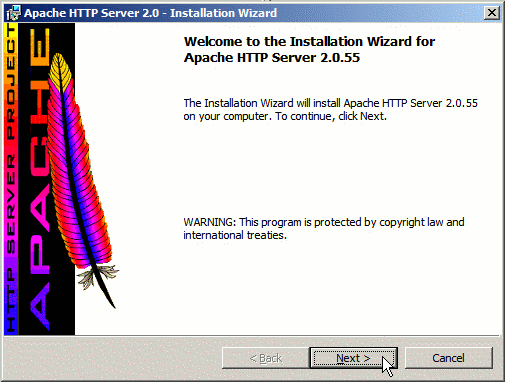
\includegraphics[scale=1,width=8cm]{ch01-01.png}
\caption{Інсталятор Apache}
\label{f1-1:image}
\end{figure}
Вам потрібно буде занести домен, в якому знаходиться сервер, ім'я сервера, e-mail адміністратора сервера. У даному випадку ці дані не важливі, їх можна залишити стандартними  (Рис.~\ref{f1-2:image}).
\begin{figure}
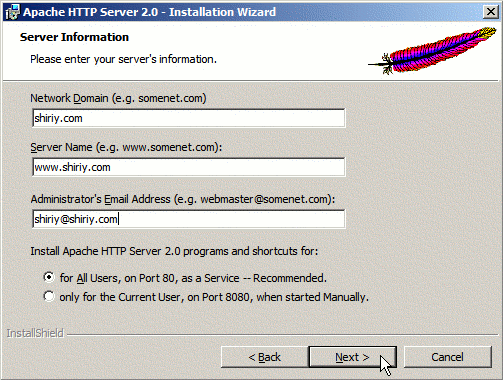
\includegraphics[scale=1,width=8cm]{ch01-02.png}
\caption{Налаштування доменних імен}
\label{f1-2:image}
\end{figure}
Також треба вибрати каталог, куди буде встановлюватися Apache, або залишити його стандартним  (Рис.~\ref{f1-3:image}). 
\begin{figure}
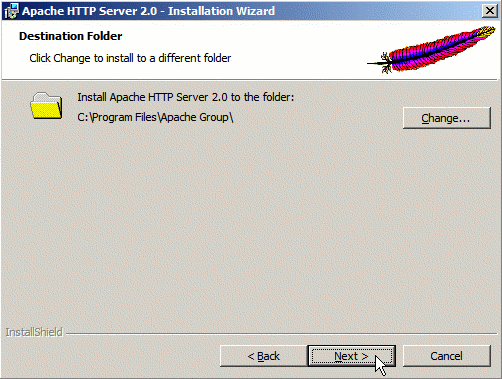
\includegraphics[scale=1,width=8cm]{ch01-03.png}
\caption{Каталог розміщення Apache}
\label{f1-3:image}
\end{figure}
Подальші зміни в конфігурації Apache можна вносити, використовуючи файл <<httpd.conf>>.

Щоб було зручно маніпулювати файлами ваших проектів створіть папку зі зрручним для вас коротким шляхом, наприклад \verb'D:\Site', в якій будуть зберігатися всі інші програми і дані сайту. Далі створіть папку \verb'D:\Site\localhost\', в якій створіть директорії WWW і CGI відповідно. WWW міститиме матеріали сайту, а CGI - скрипти CGI, якщо такі у вас будуть. В директорії \dots\verb'\Apache2\Conf\' знайдіть файл <<httpd.conf>>~--- це файл з налаштуваннями. У ньому знайдіть рядок

\begin{verbatim}
ServerRoot "C :/Program Files/Apache Group/Apache2"
\end{verbatim}

Він повинна містити шлях до самого Апач, тобто на ту папку, куди у вас Апач встановлений. Зверніть увагу, що в шляху слеш прямий і закінчується адреса без слеша.

Далі прив'язуємо Apache до конкретного порту:

\begin{verbatim}
Listen 80
\end{verbatim}

При деяких помилках сервера Apache відсилає електронні листи адміністратору, адреса поштової скриньки налаштовується у рядку

\begin{verbatim}
ServerAdmin your@email.name
\end{verbatim}

Тепер прописуємо шлях до даних сайту

\begin{verbatim}
DocumentRoot "D:/Site/localhost/WWW"
\end{verbatim}

Знайдіть блок 
\begin{verbatim}
<Directory "C:/Program Files/Apache Group/Apache2/htdocs">
\end{verbatim}

і замініть його на

\begin{verbatim}
<Directory "D:/Site">
    Options Indexes Includes
    AllowOverride All
    Order allow,deny
    Allow from all
</Directory>
\end{verbatim}

\pagebreak[3]

\section{Налаштування PHP}
\nopagebreak[4]
Встановлення PHP в середовищі Windows також не створює проблем. Завантажте встановлювач і запустіть його. 

Необхідно буде вибрати каталог для встановлення інтерпретатору, встановлену версію Apache (Рис.~\ref{f1-4:image}).
\begin{figure}
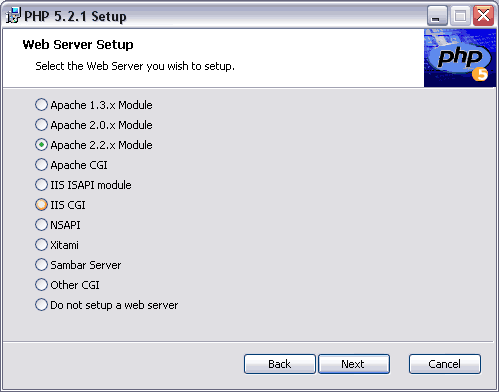
\includegraphics[scale=1,width=8cm]{ch01-04.png}
\caption{Каталог розміщення PHP}
\label{f1-4:image}
\end{figure}
Також необхідно задати місцезнаходження файлу  <<httpd.conf>> (Рис.~\ref{f1-5:image}).
\begin{figure}
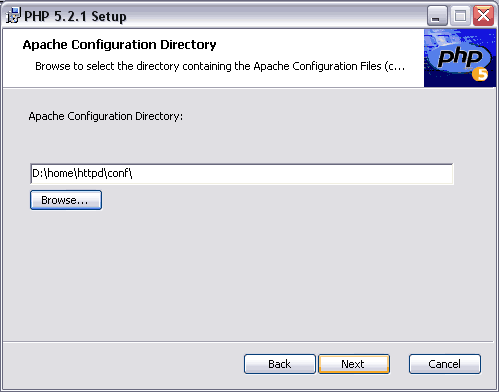
\includegraphics[scale=1,width=8cm]{ch01-05.png}
\caption{Вибір місцезнаходження файлу  <<httpd.conf>>}
\label{f1-5:image}
\end{figure}
Виберіть усі розширення PHP, що йдуть у комплекті, так ви не зіткнетесь з проблемами недостачі бібліотек під час навчання~(Рис.~\ref{f1-6:image}).

\begin{figure}
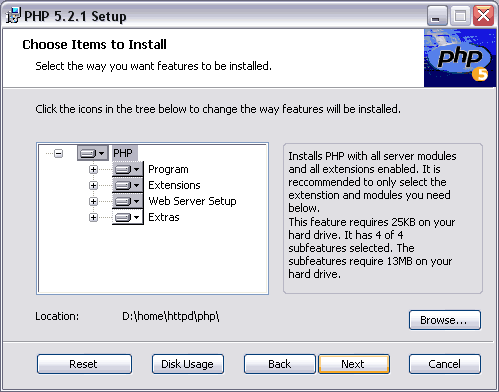
\includegraphics[scale=1,width=8cm]{ch01-06.png}
\caption{Вибір встановлюваних бібліотек}
\label{f1-6:image}
\end{figure}

У випадку проблеми прив'язки PHP до Apache його можна підключити безпосередньо у файлі <<httpd.conf>>. Для цього у файл необхідно додати такі рядки:

\begin{verbatim}
LoadModule php5_module c:/(каталог з PHP)/php5apache2_2.dll 
AddType application/x-httpd-php phtml php
PHPIniDir "c:/(каталог з PHP)/"
\end{verbatim}

Для перевірки роботи PHP та Apache створіть файл у каталозі вашого сайту <<phpinfo.php>> з такими рядками:
\pagebreak[3]
\penalty -20000
\begin{verbatim}
<?php
  echo phpinfo();
?> 
\end{verbatim}

В адресній строці браузера введіть \verb'http://localhost/phpinfo.php'. Якщо ви все виконали правильно, ви повинні побачити сторінку, зображену на Рис.~\ref{f1-7:image}:

\begin{figure}
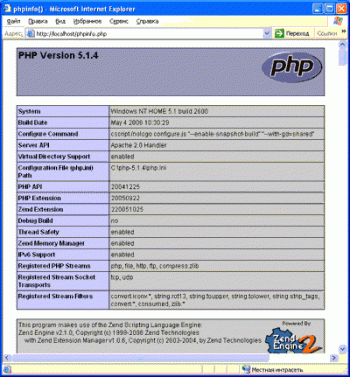
\includegraphics[scale=1,width=8cm]{ch01-07.png}
\caption{Результат роботи функції phpinfo()}
\label{f1-7:image}
\end{figure}

\pagebreak[3]

\section{Налаштування СКБД MySQL}
\nopagebreak[4]
При встановленні  СКБД MySQL вам необхідно запустити файл-інсталятор, даних за замовчуванням достатньо для встановлення повнофункціонального пакету. Після встановлення запуститься майстер налаштувань. Стандартних даних для роботи СКБД достатньо, одначе необхідно буде вказати пароль доступу адміністратора до СКБД в діалозі, зображеному на  Рис.~\ref{f1-8:image}.

\begin{figure}
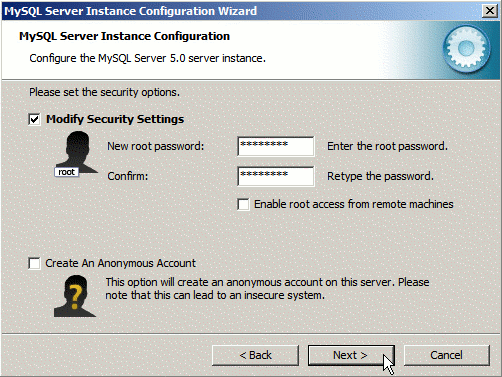
\includegraphics[scale=1,width=8cm]{ch01-08.png}
\caption{Введення пароля адміністратора СКБД}
\label{f1-8:image}
\end{figure}
Після встановлення пароля ви можете під'єднуватися до бази під логіном <<root>> та вказаним вами паролем.

\pagebreak[3]

\section{Індивідуальне завдання}
\nopagebreak[4]
\subsection*{Завдання до лабораторної роботи}
\nopagebreak[4]
\begin{enumerate}
\item Вивчити теоретичний матеріал
\item Відповісти на контрольні запитання
\item Скласти звіт
\item Захистити роботу
\end{enumerate}

\subsection*{Контрольні запитання}
\nopagebreak[4]
\begin{enumerate}
\item Що таке Internet? З яких структурних частин складається Internet?
\item Що таке IP-адреса?
\item Що таке доменне ім'я, з чого воно складається?
\item Який сервіс Internet перетворює IP-адреси в доменні імена і навпаки?
\item Яка служба займається розподіленням блоків IP-адрес?
\item Протокол HTTP. Рівень у моделі OSI, призначення.
\item Значення URI, URL, URN.
\item Мови web-програмування, які ви знаєте.
\item Веб-сервери, які ви знаєте.
\item Мережеві СКБД, які ви знаєте. 
\end{enumerate}




%\chapter{Форми HTML. Змінні, константи, масиви та функції в РНР}
\section*{Мета роботи}
Згадати основи мови розмітки веб-сторінок. Ознайомитись з базовими елементами мови РНР.
\nopagebreak[4]
\section{Формування HTML-сторінки засобами PHP}
\nopagebreak[4]
Код PHP зазвичай об'єднується з тегами XHTML. PHP є вбудовуваним мовою~--- це означає, що можна переміщатися між чистим кодом HTML і PHP, не жертвуючи можливістю читання тексту.
\index{PHP!теги відкриття/закриття}Щоб вбудувати код PHP в XHTML, PHP повинен задаватися відокремлено, за допомогою початкового та кінцевого тегів PHP. Теги PHP кажуть інтерпретатору, де починається і закінчується код PHP. Аналізатор PHP розпізнає три варіанти початкового і кінцевого тегів.

\begin{enumerate}



\item Перший варіант тегів PHP називається тегами в стилі XML і є кращим стилем. Він працює в документах розширювана мова розмітки (XML). Цей метод повинен використовуватися при з'єднанні PHP з документами XML і XHTML. Приклади в цьому підручнику застосовують цей формат тегів XML.

Стиль XML
\begin{verbatim}
<? PHP
//Блок коду PHP
>
\end{verbatim}

    
\item Скорочений стиль є найбільш простим, однак, він не рекомендується, тому що вступає в протиріччя зі стандартами документів XML та налаштуваннями в <<php.ini>>.

Скорочений стиль    
\begin{verbatim}
<?
//Блок коду PHP
>
\end{verbatim}

    
\item Цей стиль використовує найдовшу запис і схожий на стиль тегів, що застосовуються для включення кодів JavaScript. Цей стиль є кращим при використанні редактора HTML, який не розпізнає інші стилі тегів. Так як більшість нових редакторів XHTML розпізнають стиль тегів XML, то використання цього стилю не рекомендується.

Стиль сценарію
\begin{verbatim}
<script language="php">
//Блок коду PHP
</ SCRIPT>
\end{verbatim}
   
\end{enumerate}

PHP містить два основних оператора для виведення тексту в веб-браузері: \verb|echo| і  \verb|print|. Обидва оператора розміщуються між відкритим і закритим тегами блоку коду PHP і можуть перебувати в будь-якому місці в документах XHTML. Оператори  \verb|echo| і  \verb|print| використовують наступний формат:
\verb|echo|~--- використовується для виведення одного або кількох рядків.
\begin{verbatim}
echo "виведений текст";
\end{verbatim}
 \verb|print|~--- використовується для виведення рядка. В деяких випадках оператор  \verb|print| пропонує більшу функціональність, ніж оператор  \verb|echo|.
\begin{verbatim}
print "виведений текст";
\end{verbatim}
Наступні приклади демонструють використання і розміщення команд  \verb|echo| і  \verb|print| в документі XHTML.



\begin{lstlisting}[caption=Приклад вживання команд echo і print]
<!DOCTYPE html PUBLIC "-//W3C//DTD/XHTML 1.0 Transitional//EN"
  "http://www.w3.org/TR/xhtml1/DTD/xhtml11-transitional.dtd">
<html xmlns="http://www.w3.org/1999/xhtml" xml:lang="en" lang="en">
<head>
  <title> Страница Web </title>
</head>
<body>
<?php 
echo "Друк рядка оператором echo"."<br>";
print "Друк рядка оператором print";
?>
</body>
</html>
\end{lstlisting}



\pagebreak[3]
\section{Передача даних з HTML-форми PHP-сценарію}
\nopagebreak[4]
\index{HTML!передача данних}
Обробка форм є дуже важливою властивістю PHP. За допомогою форм користувачі взаємодіють зі сторінками Web, і з їхньою ж допомогою можна збирати інформацію для персоналізованих сторінок відвідувачів. У більш широкому сенсі інформаційної обробки, форми призначені для введення даних в системи обробки. Вони є первинним механізмом отримання даних, які обробляють сценарії для породження нової інформації, поновлення файлів і баз даних, а також для відповіді на запити користувачів для отримання інформації. Зовнішній вигляд типової форми дано на малюнку~\ref{f2-1:image}.

Передача даних з форм в РНР-сценарій відбувається методами  \verb|GET| або  \verb|POST| протоколу НТТР. Обидва методи однаково ефективні при використанні в формах з невеликою кількістю полів. Метод  \verb|POST| рекомендований при передачі великих обсягів тексту і файлів, обмеження за замовчуванням встановлено в 8 Мбайт і налаштовується у файлі  \verb|php.ini|.

Контейнер форми виглядає наступним чином:
\begin{verbatim}
<form name="form1" action="script.php" method="post">
</form>
\end{verbatim}
де \verb'name'~--- назва HTML-об'єкта, \verb'action' - відносний або абсолютний шлях до сценарію, якому передаються дані, \verb'method' - назва методу, яким передаються дані.

У контейнер форми поміщаються додаткові елементи управління, якими управляє користувач:

\subsection*{INPUT і його варіації}
\index{HTML!форми!input}
Елемент \verb'<input>' є найбільш вживаним тегом HTML-форм. За допомогою цього тега реалізуються основні функції форми. Він дозволяє створювати всередині форми поля введення рядка тексту, імені файлу, пароля і т.д. Також варто згадати про варіацію тега, що реалізує можливість завантаження файлів на сервер. Повний опис можливостей даного тега дано у додатку~\ref{inp-tag:app}
\subsection*{TEXTAREA}
\index{HTML!форми!textarea}
Елемент \verb'<textarea>' відповідає за передачу багаторядкового тексту. Важливо пам'ятати, що об'єм тексту, що передається обмежений параметрами методу, який використовується для передачі. Повний опис можливостей даного тега дано у додатку~\ref{tar-tag:app}
\subsection*{Списки вибору SELECT}
\index{HTML!форми!select}
Досить часто існує необхідність представити які-небудь дані у вигляді списку і передбачити можливість вибору в цьому списку. У HTML списки реалізуються за допомогою тега \verb'<select>'. Списки можуть давати можливість одиночного або множинного вибору. Повний опис можливостей даного тега дано у додатку~\ref{sel-tag:app}

\begin{figure}
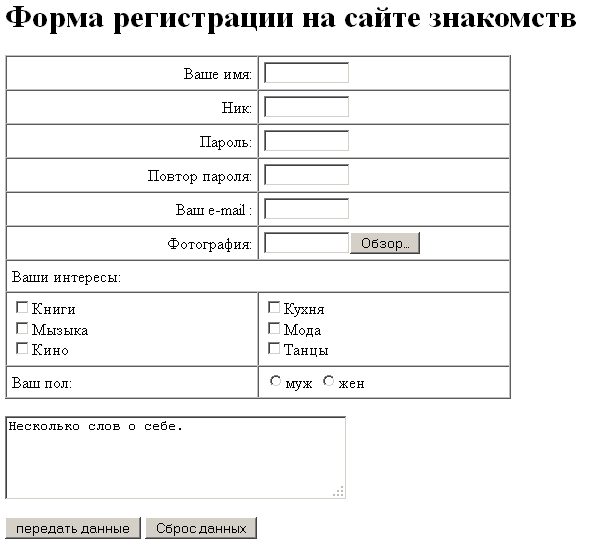
\includegraphics[scale=1,width=8cm]{ch02-01.png}
\caption{Вигляд HTML-форми}
\label{f2-1:image}
\end{figure}


\pagebreak[3]
\section{Змінні, константи та функції в РНР}
\nopagebreak[4]
\subsection*{Змінні}
\index{PHP!змінні}
\textbf{Змінні} є тимчасовим місцем зберігання, використовуваним для представлення значень в сценарії PHP. У PHP є два основні типи змінних: скалярні і масиви. Скалярні змінні містять тільки одне значення в даний момент часу, а змінні масиви - список значень. Змінні масиви обговорюються в наступному розділі. Скалярні змінні PHP містять значення типів описаних у лабораторній роботі №~\ref{datatypes}.

Імена змінних PHP всіх типів починаються зі знака <<\$>>. Імена змінних можуть містити літери, числа, і символ підкреслення (\_); вони не можуть, проте, починатися з цифри. У PHP імена змінних розрізняють регістр символів. 

\subsection*{Інтерполяція змінних}
\index{PHP!змінні!інтерполяція}
PHP підтримує також процес, званий інтерполяцією. \textbf{Інтерполяція}~--- заміна змінної в рядку її вмістом. Замість з'єднання змінних і літералів, їх можна об'єднувати всередині подвійних лапок (""). Змінні і літерали не можна об'єднати всередині одиночних лапок. При використанні подвійних лапок значення змінної виводиться разом з літералів. 
\begin{verbatim}
<?php 
$fname = "John";
$lname = "Doe";
echo "The user's name is $fname $lname";
?>
\end{verbatim}
\subsection*{Константи}
\index{PHP!константи}
\textbf{Константи}, як і змінні, є тимчасовим сховищем значень у пам'яті. На відміну від змінних значення константи ніколи не змінюється. При оголошенні константи використовується функція  \verb|define()|, яка вимагає задати ім'я константи і значення цієї константи.

Константам можна присвоювати такі типи даних.

Цілі~--- цілі числа або числа без десяткової крапки (1, 999, 325 812 841).

Числа з плаваючою точкою~--- числа, що містять десяткову крапку (1.11, 2.5, .44).

Рядки~--- текстова або числова інформація. Строкові дані завжди полягають в лапки ("Hello World", "478-477-5555").

Імена констант PHP на відміну від змінних не починаються зі знака <<\$>>. Імена констант звичайно записують у верхньому регістрі. Імена констант можуть містити літери, цифри та символ підкреслення (\_); вони не можуть, проте, починатися з цифри. Оголошення констант показано нижче.
\begin{verbatim}
define ("STRING_CONSTANT", "This is my string."); 
define ("NUMERIC_CONSTANT", 5); 
\end{verbatim}
Вивід констант подібний до виводу змінних.
\subsection*{Функції}
\index{PHP!функції}
\textbf{Функцією} називається фрагмент програмного коду, що володіє унікальним ім'ям і призначений для вирішення певного завдання. 

Функції використовуються для розбиття великих блоків коду на менші, більш керовані одиниці. Код, що міститься всередині функції, виконує певне завдання і повертає значення. PHP містить два типи функцій~--- визначені користувачем (або створені програмістом) і внутрішні (вбудовані функції), які є частиною визначення мови PHP.

Виклик вбудованої функції відбувається за допомогою її імені. Наприклад, функція, що виводить інформацію про РНР та Apache:
\begin{verbatim}
<?php
phpinfo();
?>
\end{verbatim}
У даному випадку функція викликається без параметрів. Наступна функція використовує ряд аргументів і повертає значення (у даному випадку дескриптор відкритого файлу:
\begin{verbatim}
<?php
f=fopen("d:\www\index.php","w+");
?>
\end{verbatim}
\pagebreak[3]
\section{Робота з масивами в РНР}
\nopagebreak[4]
\index{PHP!змінні!масиви}
Змінну масиву можна використовувати для зберігання множини або послідовності значень. Система PHP підтримує масиви з числовими індексами і асоціативні масиви. \textbf{Масив} в PHP є фактично впорядкованим відображенням. Відображення є типом, який відображає значення в ключі. Змінні масивів складаються з двох частин~--- індексу та елемента. Індекс масиву, іноді званий ключем масиву, є значенням, застосовуваним для ідентифікації або доступу до елементів масиву. Індекс масиву поміщається в квадратні дужки. Більшість масивів використовують числові індекси, які зазвичай починаються з 0 або 1. У PHP асоціативні масиви можуть використовувати рядкові індекси. Обидва типи масивів створюються за допомогою конструкції  \verb|array()|
\subsection*{Масиви з числовими індексами}
\begin{verbatim}
$my_array = array('red', 'green', 'blue'); 
\end{verbatim}
Цей код створює масив з числовим індексом з ім'ям \verb'$my_array'. Масиву присвоюється три елементи~---  \verb|red|,  \verb|green| і  \verb|blue|. Кожен елемент ідентифікується числовим індексом.
\begin{verbatim}
$my_array [0] = 'red' // індекс 0 відповідає елементу red 
$my_array [1] = 'green' // індекс 1 відповідає елементу green 
$my_array [2] = 'blue' // індекс 2 відповідає елементу blue 
\end{verbatim}
Щоб отримати доступ до вмісту масиву, використовується ім'я масиву та індекс. 
\subsection*{Асоціативні масиви}
Асоціативні масиви дозволяють використовувати більш корисні значення індексу. Для масивів з числовими індексами значення індексу створюються автоматично, починаючи з 0. Асоціативні масиви допускають застосування числових і строкових значень індексу.
\begin{verbatim}
$members = array('FName' => 'John', 'LName' => 'Smith', 'Age' => 50) 
\end{verbatim}
У цьому прикладі члени масиву містять три елементи, однак використовуються рядкові індекси~---  \verb|FName|,  \verb|LName| і  \verb|Age|.
\begin{verbatim}
$members ['FName'] = 'John' // індекс FName відповідає елементу John
$members ['LName'] = 'Smith' // індекс LName відповідає елементу Smith
$members ['Age'] = '50 '// індекс Age відповідає елементу 50 
\end{verbatim}
Для доступу до вмісту масиву використовується ім'я масиву та індекс.
\pagebreak[3]
\section{Функції, визначені користувачем}
\nopagebreak[4]
\index{PHP!функції!користувацькі функції}
\textbf{Визначені користувачем функції} створюються за допомогою ключового слова \verb'function'. Вони особливо корисні у великих програмах PHP, так як можуть містити блоки коду, які можуть використовуватися в програмі, що дозволяє уникнути повторного переписування коду. Далі представлений приклад простої визначеної користувачем функції PHP:
\begin{verbatim}
function AddNumbers ($num1, $num2)
{
echo "Це приклад функції PHP. 
Вона обчислює суму двох чисел і повертає 
результат програмі, що її викликала";
return $num1 + $num2;
} 
\end{verbatim}


Визначені користувачем функції можуть викликатися в будь-якому місці програми на PHP. У PHP функція виконується при використанні в коді її імені. Після виклику функція отримує всі передані їй значення у формі параметрів, виконує певні завдання і повертає значення програмі. 

\pagebreak[3]
\section{Змінні всередині функції}
\nopagebreak[4]
\index{PHP!змінні!локальні змінні}
\index{PHP!змінні!глобальні змінні}
\textbf{Глобальні змінні}~--- це змінні, які доступні всій програмі, включаючи підпрограми (користувальницькі функції).

\textbf{Локальні змінні}~--- змінні, визначені всередині підпрограми (користувацької функції). Вони доступні тільки всередині функції, в якій вони визначені.

Для PHP всі оголошені і використовувані у функції змінні за замовчуванням локальні для функції. Тобто, за умовчанням немає можливості змінити значення глобальної змінної в тілі функції. 

існує спеціальна інструкція \verb'global', що дозволяє функції користувача працювати з глобальними змінними. Розглянемо даний принцип на конкретному прикладі:

\begin{verbatim}
<?php
$a = 1 ;
$b = 2 ;

function sum()
{
global $a, $b;
$b = $a + $b;
}
?> 
\end{verbatim}

\pagebreak[3]
\section{Змінні-функції}
\nopagebreak[4]
\index{PHP!функції!змінні-функції}
PHP підтримує концепцію \textbf{змінних-функцій}. Це означає, що якщо до імені змінної приєднані круглі дужки, PHP шукає функцію з тим же ім'ям, що і результат обчислення змінної, і намагається її виконати. Цю можливість можна використовувати для реалізації зворотних викликів, таблиць функцій і безлічі інших речей.

Приклад використання змінної-функції наведено в додатку~\ref{var-func:app}

\pagebreak[3]
\section{Індивідуальне завдання}

\nopagebreak[4]
\subsection*{Завдання до лабораторної роботи}
\nopagebreak[4]
\begin{enumerate}
\item Вивчити теоретичний матеріал
\item Відповісти на контрольні запитання
\item Скласти алгоритм (блок-схему) програми
\item Виконати практичне завдання
\item Скласти звіт
\item Захистити роботу
\end{enumerate}

\subsection*{Контрольні запитання}
\nopagebreak[4]
\begin{enumerate}
\item Що таке змінні, константи та функції?
\item Що таке інтерполяція змінних?
\item Що таке масиви?
\item Як отримати доступ до індексного масиву? 
\item До ассоціативного?
\item Як створити користувацьку функцію?
\item Що таке локальні змінні?
\item Що таке глобальні змінні? Як ними користуватись у тілі функції?
\item Що таке змінні-функції?
\item Яким чином здійснюється виклик функції-змінної?
\end{enumerate}

\subsection*{Практичні завдання}
\nopagebreak[4]


\begin{enumerate}
\item[]Написати HTML-сторінку з формою, що складається з:
\item однорядкового поля вводу, поля вводу пароля та кнопки відправлення форми.
\item однорядкового поля вводу, прихованого текстового поля та кнопки відправлення форми.
\item однорядкового поля вводу, багаторядкового поля вводу та кнопки відправлення форми.
\item багаторядкового поля вводу, списку з одиночним вибором з п'яти елементів та кнопки відправлення форми.
\item прихованого текстового поля, списку з одиночним вибором з п'яти елементів та кнопки відправлення форми.
\item багаторядкового поля вводу, списку з множинним вибором з п'яти елементів та кнопки відправлення форми.
\item списку з одиночним вибором з п'яти елементів, поля вводу пароля та кнопки відправлення форми.
\item списку з множинним вибором з п'яти елементів, багаторядкового поля вводу та кнопки відправлення форми.
\item[]Отримати дані форми і вивести іх за допомогою функції в окремому сценарії.
\item створити асоціативний масив з днями тижня та вивести його на сторінку
\item створити індексний массив з назвами місяців і вивести його на екран
\item[]Написати HTML-сторінку з формою, що складається з однорядкового поля вводу та кнопки відправлення. Записати в поле число та обробити наступним чином:
\item створити константу та помножити на отримане з форми число 
\item створити змінну, занести в неї результат з форми, помножити змінну саму на себе
\item створити константу та обчислити вираз $x*const+2*x$
\item створити константу та обчислити вираз $\frac{x}{const}+x^2$
\item створити змінну та константу, в змінну занести константу і додати до числа з форми.
\item[]Результат вивести на сторінку 
\item[]Створити форму з трьома однорядковими полями і кнопкою відправлення форми
\item отримані з форми дані занести в асоціативний масив
\item отримані дані занести в індексний масив
\item[]зміст масиву роздрукувати функцією \verb'print_r()'; 
\item створити функцію, що друкує свій параметр
\item створити функцію, що перемножує два свої параметри і повертає результат. Результат роздрукувати
\item створити функцію, що перемножує свої параметри і друкує результат
\item створити функцію, що змінює глобальну змінну
\item створити функцію, що перемножує глобальну змінну і вхідний параметр, рузультат друкує
\item створити функцію, що домножує глобальну змінну на вхідний параметр і повертає результат
\item створити функцію, що формує індексний масив з двох локальних змінних і друкує його функцією \verb'print_r()';
\item створити функцію, що формує асоціативний масив з параметрів і друкує його функцією \verb'print_r()';

\end{enumerate}




%\chapter{Взаємодія PHP та web-сервера. Синтаксис PHP}
\nopagebreak[4]
\section*{Мета роботи}
Ознайомитись зі змінними оточення веб-серверу та суперглобальними масивами РНР. Ознайомитись з конструкціями розгалуження, циклів, включення файлів.
\section{Змінні оточення web-сервера Apache, суперглобальні масиви PHP}
\nopagebreak[4]

\subsection*{Змінні оточення web-сервера Apache}
\index{Web-сервери!Apache!змінні оточення}
\textbf{Змінні оточення}~--- дуже важливий механізм взаємодії веб-сервера з предобработчікамі запитів. При отриманні HTTP-запиту веб-сервер формує змінні оточення, заносячи в них різну інформацію: IP-адреса клієнта, запитуваний документ, параметри запиту і т.п. При передачі управління якомусь предобработчіку останній має доступ до змінних оточення веб-сервера, отже, йому доступна вище перерахована інформація.

Безпосередньо перед запуском сценарію сервер передає йому якісь змінні оточення з інформацією. Змінні оточення в мові PHP можна використовувати як звичайнісінькі змінні. Змінні оточення діляться на чотири великі групи:
\begin{enumerate}
\item Формовані сервером змінні;
\item Спеціальні змінні сервера Apache;
\item Змінні HTTP-полів запиту;
\item Змінні SSL-з'єднання (захищеного з'єднання).
\end{enumerate}

\subsection*{Суперглобальні масиви PHP}
\index{PHP!змінні!суперглобальні масиви}
\textbf{Суперглобальними масивами} (superglobal arrays) в PHP називаються зумовлені масиви, які видно в будь-якому місці вихідного коду без використання ключового слова \verb'global'.


Доступ до змінних оточення здійснюється через суперглобальний масив \verb'$_SERVER' у вигляді \verb|$_SERVER['змінна_CGI']|; Наприклад код
\begin{verbatim}
print $_SERVER['SERVER_SOFTWARE'];
\end{verbatim}
роздрукує в браузері строку виду:
\begin{verbatim}
Apache/2.2.4 (Win32) mod_ssl/2.2.4 OpenSSL/0.9.8k PHP/5.3.3
\end{verbatim}


Повний перелік змінних оточення web-сервера Apache та суперглабальних масивів PHP дивіться у додатках~\ref{var-apa:app} та~\ref{sup-glob:app}.


\pagebreak[3]



\section{Оператори PHP}
\nopagebreak[4]
\index{PHP!оператори}
Синтаксис PHP дуже нагадує синтаксис мови C і багато в чому запозичений з таких мов як Java і Perl. Інструкції поділяються також як і в C або Perl~--- кожен вираз закінчується крапкою з комою. Закриваючий тег <<?> >> також має на увазі кінець інструкції.

Коментарі застосовуються в PHP для запису власних зауважень під час процесу розробки коду. Такі коментарі можуть визначати призначення сегмента коду або їх можна використовувати для виключення блоків коду під час тестування і налагодження сценаріїв.

Синтаксичний аналізатор PHP ігнорує коментарі. Коментарі в PHP можна визначити одним з наступних способів:
\begin{enumerate}

\item \verb|//|~--- Простий коментар PHP;
\item \verb|#|~--- Альтернативний простий коментар PHP;
\item \verb|/* ... */|~--- Багаторядкові блоки коментарів.

\end{enumerate}
\penalty -10000
Імена змінних позначаються знаком \$.

\begin{verbatim}
<?php
$message = "Привет, я - скрипт PHP!";
echo $message;
?>
\end{verbatim}
\index{PHP!змінні!типи даних}
PHP підтримує вісім простих типів даних \label{datatypes}:
\begin{enumerate}
\item Чотири скалярних типи:
		\begin{itemize}
		\item Boolean (двійкові дані)
		\item Integer (цілі числа)
		\item Float (числа з плаваючою точкою або 'double')
		\item String (рядки)
		\end{itemize}
\item Два змішаних типи:
		\begin{itemize}
		\item Array (масиви)
		\item Object (об'єкти)
		\end{itemize}
\item Два спеціальних типи:
		\begin{itemize}
		\item resource (ресурси)
		\item NULL (<<порожні>>)
		\end{itemize}
\item Існують також кілька псевдотіпов:
		\begin{itemize}
		\item Mixed (змішані)
		\item Number (числа)
		\item Callback (зворотний визов)		
		\end{itemize}
\end{enumerate}

Основними конструкціями мови PHP є:
\index{PHP!конструкції}
\begin{enumerate}
\item Умовні оператори (\verb|if, else|);
\item Цикли (\verb|while, do-while, for, foreach, break, continue|);
\item Конструкції вибору (\verb|switch|);
\item Конструкції оголошення (\verb|declare|);
\item Конструкції повернення значень (\verb|return|);
\item Конструкції включень (\verb|require, include|).
\end{enumerate}


Для здійснення операцій зі змінними існують різні групи операторів. Оператором називається дещо, що складається з одного або більше значень (виразів), яке можна обчислити як нове значення (таким чином, вся конструкція може розглядатися як вираз).

\textbf{Оператори бувають трьох видів.}
\begin{enumerate}
\item Унарні оператори, які працюють тільки з одним аргументом, наприклад, <<!>> (оператор заперечення) або <<++>> (інкрімент).
\item Бінарні оператори: до них належать більшість підтримуваних в PHP операторів
\item тернарних оператор <<\dots?\dots:\dots>>. Він використовується для умовного вибору між двома операторами, в залежності від результату обчислення третього оператора.
\end{enumerate}
\subsection*{Пріоритет виконання операторів}
\index{PHP!оператори!пріоритети}
Пріоритет операторів визначає, в якому порядку будуть обчислюватися два і більше вирази. Наприклад, вираз $1 + 5 * 3$ обчислюється як 16, а не 18, оскільки операція множення <<*>> має більш високий пріоритет, ніж операція додавання <<+>>. У разі, якщо оператори мають однаковий пріоритет, вони будуть виконуватися зліва направо. Круглі дужки можуть використовуватися для примусового вказівки необхідного порядку виконання операторів. Наприклад, вираз $(1 + 5) * 3$ обчислюється як 18.

В таблиці~\ref{pr-op:table} додатку надано пріоритети виконання операторів PHP.

Ліва асоціативність вказує на те, що вираз обчислюється зліва направо, права асоціативність відповідно має увазі протилежний порядок.
\pagebreak[3]
\section{Конструкції вибору}
\index{PHP!конструкції!розгалуження}
\nopagebreak[4]
До конструкцій вибору відносять: умовний оператор (\verb'if...else') і перемикач (\verb'switch'). 
\subsection*{if \dots else}
Синтаксис умовного оператора:
\begin{verbatim}
if (condition) statement1 else statement2
\end{verbatim}


Умова \verb'condition' може бути будь-яким виразом. Якщо \verb'condition' істинне, то виконується оператор \verb'statement1' . В іншому випадку виконується оператор \verb'statement' 2. Допустима скорочена форма запису умовного оператора, в якій відсутні \verb'else' і оператор \verb'statement2'.

У свою чергу, оператори \verb'statement1' і \verb'statement2' можуть бути умовними, що дозволяє організовувати послідовність перевірок будь-якої глибини вкладеності. І в цих послідовностях кожен умовний оператор може бути як повним, так і скороченим. У зв'язку з цим можливі помилки неоднозначного зіставлення \verb'if' і \verb'else'.

Зауважимо, що перевірка додаткових умов можлива за допомогою оператора \verb|elseif|. Оператор \verb|if| може включати скільки завгодно блоків \verb'elseif', але else в кожному if може бути тільки один. Як правило, в конструкціях \verb'if ... elseif ... else' оператор else визначає, що потрібно робити, якщо ніякі інші умови не є true. 

РНР надає також можливість альтернативного синтаксису умовного оператора~--- без фігурних дужок, а із застосуванням оператора \verb'endif', при цьому оператори будуть розміщені всередині блока.

\subsection*{Перемикач <<switch>>}

Перемикач \verb'switch' є найбільш зручним засобом для організації множинного розгалуження. Синтаксис перемикача такий:
\penalty -10000
\begin{verbatim}
switch (expression) 
{
case value1: statements; break;
case value2: statements; break;
default:
statements;
}
\end{verbatim}

Керуюча структура \verb'switch' передає керування тому з помічених \verb'case' операторів, для якого значення константного виразу збігається зі значенням \verb'expression'. Якщо значення \verb'expression' не збігається ні з одним з константних виразів, то виконується перехід до оператора, поміченого міткою \verb'default'. У кожному перемикачі може бути не більше однієї мітки \verb'default', однак вона може бути відсутньою взагалі.


\pagebreak[3]

\section{Конструкції циклів}
\nopagebreak[4]

\index{PHP!конструкції!цикли}

На другому місці за частотою використання, після конструкцій умов (умовних операторів), знаходяться цикли.

Цикли дозволяють повторювати певну (і навіть невизначений~--- коли робота циклу залежить від умови) кількість разів різні послідовності операторів. Дані оператори називаються тілом циклу. Прохід циклу називається ітерацією.

PHP підтримує чотири види циклів:
\begin{itemize}
\item    Цикл з передумовою (while)
\item    Цикл з постусловіем (do-while)
\item    Цикл з лічильником (for)
\item    Спеціальний цикл перебору масивів (foreach)
\end{itemize}

Цикли зручно також використовувати при форматуванні HTML-сторінки. Наприклад при створенні великих списків або таблиць.

\begin{lstlisting}[caption=Формування HTML-сторінки за допомогою циклів]
<!DOCTYPE html PUBLIC "-//W3C//DTD/XHTML 1.0 Transitional//EN"
  "http://www.w3.org/TR/xhtml1/DTD/xhtml11-transitional.dtd">
<html xmlns="http://www.w3.org/1999/xhtml" xml:lang="en" lang="en">
<head>
  <title> Страница Web </title>
</head>
<body>
<table>
<?php
for (int $i=1; $i<=10; $i++) 
echo "<tr><td> Рядок № </td><td>$i</td></tr>\n";
?>
</table>
</body>
</html>
\end{lstlisting}




Сценарій для тієї самої сторінки без використання циклів зайняв б у два рази більше дискового простору.

При використанні циклів є можливість використання операторів \verb'break' і \verb'continue'. Перший з них перериває роботу всього циклу, а другий~--- тільки поточної ітерації.


\subsection*{Цикл з передумовою while}
\index{PHP!конструкції!while}
Цикл з передумовою while працює за такими принципами:

\begin{enumerate}
\item    Обчислюється значення логічного виразу.
\item    Якщо значення істинно, виконується тіло циклу, в іншому випадку~--- переходимо на наступний за циклом оператор.
\end{enumerate}


Синтаксис циклу з передумовою:
\begin{verbatim}
while (логічний_вираз) інструкція;
\end{verbatim}

В даному випадку тілом циклу є інструкція. Зазвичай тіло циклу складається з великої кількості операторів. Наведемо приклад циклу з передумовою while:
\begin{verbatim}
<? Php
$х = 0;
while ($x++<10) echo $x;
// Виводить 12345678910
?>
\end{verbatim}
Зверніть увагу на послідовність виконання операцій умови \$x++<10. Спочатку перевіряється умова, а тільки потім збільшується значення змінної. Якщо ми поставимо операцію інкремента перед змінної (++\$x<10), то спочатку буде виконано збільшення змінної, а тільки потім~--- порівняння. У результаті ми отримаємо рядок <<123456789>>. 


Подібно конструкції умовного оператора \verb'if', можна групувати оператори всередині тіла циклу while, використовуючи наступний альтернативний синтаксис:
\begin{verbatim}
while (логічний_вираз):
інструкція;
...
endwhile;
\end{verbatim}

\subsection*{Цикл з постумовою do while}
\index{PHP!конструкції!do while}
На відміну від циклу \verb'while', цей цикл перевіряє значення виразу не до, а після кожного проходу (ітерації). Таким чином, тіло циклу виконується хоча б один раз. Синтаксис циклу з постумовою такий:
\begin{verbatim}
do
{
тело_цікла;
}
while (логічний_вираз);
\end{verbatim}
Після чергової ітерації перевіряється, чи істинний \verb'логічний_вираз', і, якщо це так, управління передається знову на початок циклу, в іншому випадку цикл обривається.

\subsection*{Цикл з лічильником <<for>> (регулярний цикл)}
\index{PHP!конструкції!for}
Цикл з лічильником використовується для виконання тіла циклу певне число разів. 

Синтаксис циклу \verb'for' такий:
\begin{verbatim}
for (ініціалізуючі_команди; умова_роботи; 
	команди_після_ітерації) {тіло_цикла;}
\end{verbatim}
Цикл for починає свою роботу з виконання \verb'ініціалізуючіх_команди'. Дані команди виконуються тільки один раз. Після цього перевіряється \verb'умова_роботи', якщо воно істинно (true), то виконується \verb'тіло_цикла'. Після того, як буде виконаний останній оператор тіла, виконуються \verb'команди_після_ітерації'.



Для циклу for є і альтернативний синтаксис:
\begin{verbatim}
for (ініціалізуючі_команди; умова_роботи; 
команди_після_ітерації):
оператори;
endfor;
\end{verbatim}

\subsection*{Цикл перебору масивів <<foreach>>}
\index{PHP!конструкції!foreach}
В PHP4 з'явився ще один спеціальний тип циклу~--- \verb'foreach'. Даний цикл призначений спеціально для перебору масивів.

Синтаксис циклу \verb'foreach' виглядає наступним чином:
\begin{verbatim}
foreach (масив as $ключ => $значення)
команди;
\end{verbatim}
Тут команди циклічно виконуються для кожного елемента масиву, при цьому чергова пара <<ключ => значення>> виявляється в змінних \verb'$ключ' і \verb'$значення'. 

У циклу foreach є й інша форма запису, яку слід застосовувати, коли нас не цікавить значення ключа чергового елемента. Виглядає вона так:
\begin{verbatim}
foreach (масив as $значення)
команди;
\end{verbatim}
У цьому випадку доступно лише значення чергового елементу масиву, але не його ключ. Це може бути корисно, наприклад, для роботи з масивами-списками:



Увага: Цикл \verb'foreach' оперує не вихідним масивом, а його копією. Це означає, що будь-які зміни, які вносяться в масив, не можуть бути <<видимі>> з тіла циклу. Що дозволяє, наприклад, в якості масиву використовувати не тільки змінну, але і результат роботи якої-небудь функції, що повертає масив (у цьому випадку функція буде викликана всього один раз~--- до початку циклу, а потім робота буде проводитися з копією повернутого значення).

\subsection*{Конструкція <<break>>}
\index{PHP!конструкції!break}
Дуже часто для того, щоб спростити логіку якого-небудь складного циклу, зручно мати можливість його перервати в ході чергової ітерації (наприклад, при виконанні якого-небудь особливого умови). Для цього і існує конструкція break, яка здійснює негайний вихід з циклу. Вона може задаватися з одним необов'язковим параметром~--- числом, яке вказує, з якого вкладеного циклу має бути здійснений вихід. За замовчуванням використовується 1, тобто вихід з поточного циклу, але іноді застосовуються й інші значення. Синтаксис конструкції \verb'break':
\begin{verbatim}
break; // За замовчуванням
break (номер_цикла); // Для вкладених циклів 
(вказується номер циклу, що переривається)
\end{verbatim}

\subsection*{Конструкція <<continue>>}
\index{PHP!конструкції!continue}
Конструкція \verb'continue' так само, як і \verb'break', працює тільки <<в парі>> з циклічними конструкціями. Вона негайно завершує поточну ітерацію циклу та переходить до нової (звичайно, якщо виконується умова циклу для циклу з передумовою). Точно так само, як і для \verb'break', для continue можна вказати рівень вкладеності циклу, який буде продовжений з повернення управління.


\pagebreak[3]

\section{Конструкції включення}
\nopagebreak[4]
Конструкції включень дозволяють збирати PHP програму (скрипт) з декількох окремих файлів.

У PHP існують дві основні конструкції включень: \verb'require' і \verb'include'.
\subsection*{Конструкція включень <<require>>}
\index{PHP!конструкції!require}
Конструкція \verb'require' дозволяє включати файли в сценарій PHP до виконання сценарію PHP. Загальний синтаксис \verb'require' такий:
\begin{verbatim}
require им'я_файлу;
або
require (им'я_файлу);
\end{verbatim}
При запуску (саме при запуску, а не при виконанні!) Програми інтерпретатор просто замінить інструкцію на вміст файлу \verb|им'я_файлу| (цей файл може також містити сценарій на PHP, обрамлений, як зазвичай, тегами << <? >> та << ?> >>'). Причому зробить він це безпосередньо перед запуском програми (на відміну від include , який розглядається нижче). Це буває досить зручно для включення в висновок сценарію різних шаблонних сторінок HTML-кодом. 
\subsection*{Конструкція <<include>>}
\index{PHP!конструкції!include}
Конструкція \verb'include' також призначена для включення файлів в код сценарію PHP.

На відміну від конструкції \verb'require' конструкція \verb'include' дозволяє включати файли в код PHP скрипта під час виконання сценарію. Синтаксис конструкції \verb'include' виглядає наступним чином:
\penalty -10000
\begin{verbatim}
include им'я_файлу;
або
include (им'я_файлу);
\end{verbatim}

Принципова різниця між цими двома операторами в тому, що \verb'include' дозволяє включати файли <<на літу>>, і робити це декілька разів, наприклад у циклах.
\subsection*{Конструкції одноразового включення <<require\_once>> і <<include\_once>>}
\index{PHP!конструкції!require\_once} \index{PHP!конструкції!include\_once}
У великих PHP сценаріях інструкції \verb'include' і \verb'require' застосовуються дуже часто. Тому стає досить складно контролювати, як би випадково не включити один і той же файл декілька разів, що найчастіше призводить до помилки, яку складно виявити.

У PHP передбачено вирішення даної проблеми. Використовуючи конструкції одноразового включення \verb'require_once' і \verb'include_once', можна бути впевненим, що один файл не буде включено двічі. Працюють конструкції одноразового включення \verb'require_once' і \verb'include_once' так само, як і \verb'require' і \verb'include' відповідно. Різниця в їх роботі лише в тому, що перед включенням файлу інтерпрететор перевіряє, чи включений вказаний файл раніше чи ні. Якщо так, то файл не буде включено знову. 

\subsection*{Включення віддалених файлів}

Конструкції однократних включень \verb'require_once' і \verb'include_ince' також дозволяють включати віддалені файли, якщо така можливість включена в конфігураційному файлі PHP.

Якщо \verb'URL fopen' увімкнено в PHP (як у конфігурації за замовчуванням), ви можете специфікувати файл, що підключається з використанням URL (через HTTP), замість локального шляху. 

Для того, щоб віддалене включення файлів було доступно, необхідно в конфігураційному файлі (php.ini) встановити \verb'allow_url_fopen = 1'.


\pagebreak[3]

\section{Конструкція <<or exit()>> (<<or die()>>)}
Конструкція складається з логічного оператора \verb'or' та функції \verb'exit()' або її псевдоніма \verb'die()'. Функція \verb'exit(статус)' друкує на екрані статус, котрий може бути цілочисельною або рядковою константою. Конструкцію зручно використовувати під час налагодження сценаріїв у комбінації з функціями, які можуть повертати логічне \verb'FALSE'. Наприклад зупинку сценарію при невдалому відкритті файлу можна отримати таким чином:
\begin{verbatim}
$file = fopen("file.txt","w+") or die("Помилка відкриття файлу");
\end{verbatim} 



\pagebreak[3]

\section{Індивідуальне завдання}

\nopagebreak[4]
\subsection*{Завдання до лабораторної роботи}
\nopagebreak[4]
\begin{enumerate}
\item Вивчити теоретичний матеріал
\item Відповісти на контрольні запитання
\item Скласти алгоритм (блок-схему) програми
\item Виконати практичне завдання
\item Скласти звіт
\item Захистити роботу
\end{enumerate}

\subsection*{Контрольні запитання}
\nopagebreak[4]
\begin{enumerate}
\item Які оператори виводу тексту ви знаєте?
\item Які групи змінних оточення ви знаєте?
\item Що таке суперглобальні масиви, як ними користуватись?
\item Яким чином можна задати коментар?
\item Які типи операторів ви знаєте?
\item Які конструкції вибору ви знаєте?
\item Які конструкції циклів ви знаєте?
\item У якому випадку цикл виконується хоча-б один раз?
\item Якими чином можна включити інший текстовий файл у сценарій?
\item Яка особливість операторів <<include\_once>> та <<require\_once>>? 
\end{enumerate}

\subsection*{Практичні завдання}
\nopagebreak[4]


\begin{enumerate}
 
\item[]Створити окремий РНР-файл, підключити його у головну сторінку. Файл повинен:
\item У регулярному циклі виводити числа від 1 до 20
\item У циклі з передумовою виводити числа від 20 до 50
\item У циклі з постумовою вивести числа від -50 до -10
\item Використовуючи регулярний цикл вивести елементи арифметичної прогресії з 20 елементів починаючи з 1 та доданком 2
\item Використовуючи з передумовою вивести елементи геометричної прогресії з 20 елементів починаючи з 1 та доданком 2
\item Розрахувати факторіал 10 за допомогою регулярного циклу
\item Вивести латинський алфавіт, використовуючи регулярний цикл
\item Вивести латинський алфавіт, використовуючи цикл з передумовою
\item Вивести Цифри від 20 до 0 у зворотньому порядку, використовуючи цикл з постумовою.
\item[]Написати HTML-сторінку з формою, що складається з однорядкового поля вводу та кнопки відправлення форми. В поле вводу ввести число та обчислити вираз: 
\item якщо $x>0$ то $5*x^2 + 2*x - 10$, інакше $5*x^2 + 2*x + 10$
\item якщо $0<x\le 10$ то $10*x^3 - 2*x - 10$, інакше $x^2 + 20*x$
\item якщо $0<x\le 20$ то $\frac{x}{x+1} + 2*x - 10$, інакше $\frac{x+1}{x} + 10$
\item якщо $-10<x\le 0$ то $5*x^2 + 2*x - 10$, $x> 0$ $5*x^2 + 2*x + 10$, інакше $\frac{x+1}{x} + 10$
\item якщо $x\le 10$ то $x^3 + 2*x^2$, інакше $2*x + 10$
\item якщо $x>10$ то $5*x^2 + \frac{x}{2}$, інакше $\frac{x+10}{x+1}$
\item[]Написати HTML-сторінку з формою, що складається з однорядкового поля вводу та кнопки відправлення форми. В поле вводу ввести число та використовуючи конструкцію <<switch-case>>: 
\item за номером дня тижня вивести його назву.
\item за номером місяця року вивести його назву.
\item від 0 до 10 вивести назви цифр
\item відповідно номера вивести букву латинського алфавіту
\item[]Опрацювати змінні оточення 
\item вивести шлях до каталогу з веб-документами
\item вивести підпис веб-сервера
\item вивести інформацію про браузер користувача
\item вивести адресу електронної пошти адміністратора
\item за допомогою конструкції перебору масивів вивести зміст \$\_SERVER
\item за допомогою конструкції перебору масивів вивести зміст \$\_ENV

\end{enumerate}

%\chapter{Робота з рядками. Регулярні вирази}
\section*{Мета роботи}
Ознайомитись із засобами роботи з рядковими змінними та константами. Ознайомитись із застосуванням регулярних виразів у мові РНР та SQL-запитах.
\nopagebreak[4]
\section{Рядки. Функції роботи з рядками}
\nopagebreak[4]
\index{PHP!змінні!рядки}
\textbf{Рядки є послідовностями символів}. У PHP символ відповідає байту, тобто існує точно 256 можливих різних символів. Рядки можуть бути дуже великими. У PHP не існує практичного обмеження на розмір рядків, тому взагалі немає причин турбуватися про їх довжині. Строкові значення можуть використовуватися буквально або присвоюватися змінним.

У PHP рядковий літерал можна задати трьома способами.
\begin{itemize}
\item рядки в одиночних лапках
\item рядки в подвійних лапках
\item рядки в синтаксисі heredoc 
\end{itemize}

\subsection*{Рядки в одиночних лапках}
Одиночні лапки надають найпростіший метод для роботи з рядками. При використанні цього методу рядки укладаються в одиночні лапки <<''>>. Якщо одиночні лапки потрібні як частина рядка, вони повинні бути екрановані символом зворотної косої межі <<\\>>. Хоча одиночні лапки надають простий спосіб роботи з рядками, одиночні лапки не підтримують застосування інтерполяції.
\subsection*{Рядки в подвійних лапках}
Рядки PHP можна виводити також за допомогою подвійних лапок <<"">>. Якщо рядки PHP поміщаються в подвійні лапки, то можна застосовувати інтерполяцію. Для рядків у подвійних лапках PHP підтримує також більшість екранованих символів. Ці символи представлені в таблиці~\ref{doub-lap:table} нижче.

\begin{center}
\begin{longtable}[t]{|l|p{20em}|}
\caption{Екрановані символи у подвійних лапках} \label{doub-lap:table}\\
\hline
Символ & Опис \\
\hline
\verb'\N' & перенесення рядка \\
\verb'\R' & повернення каретки \\
\verb'\T' & горизонтальна табуляція \\
\verb'\\' & зворотна коса риска \\
\verb'\$' & знак долара \\
\verb'\"' & подвійні лапки \\
\hline
\end{longtable}
\end{center}

\subsection*{Рядки в синтаксисі heredoc}
\textbf{Heredoc}-синтаксис~--- спосіб визначення строкових змінних у вихідному коді програм.

При визначенні строкових змінних їх вміст, зазвичай, полягає в одинарні або подвійні лапки, у зв'язку з чим символи лапок, які повинні бути частиною даних, доводиться екранувати за допомогою escape-послідовностей. Heredoc-синтаксис дозволяє визначити рядок, не укладаючи її в лапки, у зв'язку з чим необхідність екранування цих символів відпадає.

Приклад використання такого синтаксису наведено нижче:
\begin{verbatim}
$S = << EOL; 
Лапки бувають 'одинарними' і "подвійними". 
EOL
\end{verbatim} 
\subsection*{Функції роботи з рядками}
\index{PHP!змінні!рядки!функції}
У базовому наборі РНР існує величезна кількість функцій для обробки рядків. Як правило іх достатньо для написання програм, іноді необхідно комбінувати ці функції між собою для отримання необхідного результату. Повний перелік функцій дан у таблиці~\ref{str-func:table} додатків.

\pagebreak[3]
\section{Рядки, що включають HTML-код}
\nopagebreak[4]

\index{PHP!змінні!HTML-рядки}Досить часто ми працюємо з рядками, що містять html-теги. Якщо відобразити такий рядок в браузері за допомогою звичайних функцій відображення даних \verb'echo()' або \verb'print()', то ми не побачимо самих html-тегів, а отримаємо відформатовану у відповідності з цими тегами сторінку. Браузер обробляє всі html-теги у відповідності зі стандартом мови HTML. Іноді нам потрібно бачити безпосередньо рядок, без обробки його браузером. Щоб цього досягти, потрібно перед тим, як виводити, застосувати до рядка функцію \verb'htmlspecialchars()'.

\pagebreak[3]
\section{Регулярні вирази}
\nopagebreak[4]
\index{PHP!регулярні вирази}
\textbf{Регулярний вираз} (regular expression)~--- це технологія, яка дозволяє задати шаблон і здійснити пошук даних, відповідних цьому шаблону, в заданому тексті, представленому у вигляді рядка. Одне з поширених застосувань регулярних виразів~--- це перевірка рядка на відповідність будь-яким правилам.

Приклад регулярного виразу:
\begin{verbatim}
/^\w+([\.\w]+)*\w@\w((\.\w)*\w+)*\.\w{2,3}$/
\end{verbatim}
Основна перевага РВ полягає в тому, що вони дозволяють організувати більш гнучкий пошук, тобто знайти те, про що немає точного знання, але є приблизне уявлення. Наприклад, потрібно знайти всі семизначні номери телефонів, що зустрічаються в тексті. Ми не шукаємо якийсь заздалегідь відомий нам номер телефону, ми знаємо тільки, що шуканий номер складається з семи цифр. Для цього можна скористатися наступним РВ:

\begin{verbatim}
/\d{3}-\d{2}-\d{2}/m
\end{verbatim}

Одним з основних метасимволів є зворотний слеш <<\\>>. Він змінює тип символу, наступного за ним, на протилежний, тобто якщо це був звичайний символ, то він МОЖЕ перетворитися в метасимвол, якщо це був метасимвол, то він втрачає своє спеціальне значення і стає звичайним символом (це потрібно для того, щоб вставляти в текст спеціальні символи як звичайні). Наприклад, символ <<d>> в звичайному режимі не має ніяких спеціальних значень, але <<\\d>> є метасимволом, що означає "будь-яка цифра". Символ <<.>> в звичайному режимі означає будь одиничний символ, а <<\\.>> означає просто крапку.

Результати використання зворотнього слеша надано у таблиці\index{PHP!регулярні вирази!слеш-комбінації}:
\begin{center}
\begin{longtable}[t]{|l|p{20em}|}
\kill
\caption{\space Використання зворотнього слеша у регулярних виразах} \label{chr-meta:table}\\
\hline

Символ & Значення \\
\hline \endfirsthead
\caption*{\space Продовження} \\
\hline
Символ & Значення \\
\hline \endhead
\hline \endfoot
\verb'\n' & cимвол перекладу рядка \\

\verb'\e' & символ escape \\

\verb'\t' & cимвол табуляції \\

\verb'\Xhh' & символ в шістнадцятковому коді, наприклад \verb'\x41' є буква A і т.д. \\

\verb'\d' & будь-яка десяткова цифра (0-9) \\

\verb'\D' & будь-який символ, який не є десятковим цифрою \\

\verb'\s' & будь-який порожній символ (пробіл або табуляція) \\

\verb'\S' & будь-який символ, який не є порожнім \\

\verb'\w' & символ, використовуваний для написання Perl-слів (це літери, цифри та символ підкреслення), так званий "словниковий символ" \\

\verb'\W' & знайдене символ (всі символи, крім обумовлених \verb'\w') \\ 
\hline
\end{longtable}
\end{center}

Приклад використання наведених вище метасимволів:

\begin{verbatim}
/\d\d\d plus \d is \w\w\w/
\end{verbatim}

Цей регулярний вираз означає: тризначне число, за яким слідує підрядок \verb'plus', будь-яка цифра, потім \verb'is' і слово з трьох словникових символів. Зокрема, даним РВ задовольняють рядки: <<\verb'123 plus 3 is sum'>>, <<\verb'213 plus 4 is 217'>>.

\pagebreak[3]
\section{Функції PHP для роботи з регулярними виразами}
\nopagebreak[4]
\index{PHP!регулярні вирази!функції}
Основні функції для роботи з Perl-сумісними регулярними виразами: \verb'preg_match(pattern, string, [result, flags])' і \verb'preg_match_all(pattern, string, result, [flags])', де:

\verb'pattern'~--- шаблон регулярного виразу;

\verb'string'~--- рядок, в якій проводиться пошук;

\verb'result'~--- містить масив результатів (нульовий елемент масиву містить відповідність всьому шаблоном, перший~--- першому <<захопленому>> підшаблону і т.д.);

\verb'flags'~--- необов'язковий параметр, що визначає те, як впорядковані результати пошуку.

Ці функції здійснюють пошук за шаблоном і повертають інформацію про те, скільки разів відбувся збіг. Для \verb'preg_match()' це O (немає збігів) або 1, оскільки пошук припиняється, як тільки знайдено перший збіг. Функція \verb'preg_match_all()' робить пошук до кінця рядка і тому знаходить всі збіги. Всі точні збіги містяться в першому елементі масиву result у кожної з цих функцій (для \verb'preg_match_all()' цей елемент~--- теж масив). 
Аналогом \verb'preg_match' є булева функція POSIX-розширення \verb'ereg(string pattern, string string [, array regs])'

Функція \verb'ereg()' повертає \verb'TRUE', якщо збіг знайдено, і \verb'FALSE'~--- у противному випадку.

Наведені далі приклади можна тестувати на перерахованих функціях. Наприклад, так:



\begin{lstlisting}[caption=Приклад роботи з регулярними виразами]
<?
//Рядок, в якому потрібно щось знайти
$str = "Мій телефонний номер:".
"33-22-44. Номер мого редактора:".
"222-44-55 та 323-22-33";
//Шаблон, по якому шукати.
//Задає пошук семизначних номерів.
$pattern = "/\d{3}-\d{2}-\d{2}/m";
//Функція, що здійснює пошук
$num_match = preg_match_all($pattern, $str, $result);
//Вивід результатів пошуку
for ($i = 0; $i <$num_match; $i++) 
echo "Збіг $i:".$result[0][$i]."<br>";
?>
\end{lstlisting}






\pagebreak[3]
\section{Регулярні вирази в SQL-запитах}
\nopagebreak[4]
\index{MySQL!SQL!регулярні вирази}
Більшість сучасних СУБД також підтримують регулярні вирази. Це буває корисним коли необхідно отримати або змінити дані в базі, що відповідають певному шаблону.

В MySQL використовується розширена версія  реалізації регулярних виразів, яка орієнтована на відповідність POSIX 1003.2. Це розширена версія, в якій підтримуються операції порівняння із зразком, використовуючи оператор \verb'REGEXP' в операторах SQL.

Наприклад запит \verb|SELECT * FROM tab WHERE text REGEXP "B[an]*s"| поверне рядки <<Bananas>> та <<Baaaaas>>, якщо такі є в таблиці бази даних.

Перелік метасимволів, що підтримує MySQL, дано в таблиці~\ref{chr-rxp:table} додатків.

Альтернативою \verb'REGEXP' може виступати оператор \verb'RLIKE'. Оператор \verb'RLIKE' можна використовувати з запереченням \verb'NOT RLIKE'~--- в цьому випадку результатом його роботи буде вибірка рядків не відповідають заданим параметрам.
\pagebreak[3]
\section{Індивідуальне завдання}

\nopagebreak[4]
\subsection*{Завдання до лабораторної роботи}
\nopagebreak[4]
\begin{enumerate}
\item Вивчити теоретичний матеріал
\item Відповісти на контрольні запитання
\item Скласти алгоритм (блок-схему) програми
\item Виконати практичне завдання
\item Скласти звіт
\item Захистити роботу
\end{enumerate}

\subsection*{Контрольні запитання}
\nopagebreak[4]
\begin{enumerate}
\item Що таке рядки?
\item Яким чином можна задати рядковий літерал?
\item Яка особливість рядків у подвійних лапках?
\item Яка особливість синтаксису \verb'Heredoc'? 
\item Яким чином вивести HTML-код на веб-сторінці?
\item Що таке регулярні вирази?
\item Яка особливість метасимволу <<\verb'\'>>?
\item Для чого використвуються регулярні вирази?
\item Які функції для роботи з регулярними виразами ви знаєте?
\item Яким чином можна використовувати регулярні вирази в SQL-запитах?
\end{enumerate}

\subsection*{Практичні завдання}
\nopagebreak[4]


\begin{enumerate}
\item[]Створити HTML-форму з трьома однорядковими полями вводу та обробити інформацію у сценарії наступним чином:
\item у рядку \No1 знайти всі місця входження рядків \No\No2 та 3
\item до рядка \No1 додати рядок \No2 та знайти входження рядка \No3 в отриманому
\item у рядку \No1 знайти входження об'єднаних рядків \No2 та \No3
\item у рядку \No1 замінити перше попадання рядку \No2 на рядок \No3
\item у рядку \No1 замінити останнє попадання рядку \No2 на рядок \No3
\item у рядку \No1 замінити всі попадання рядку \No2 на рядок \No3
\item видалити пробіли на початку та кінцях усіх рядків
\item у рядку \No1 видалити HTML-теги, рядок \No2 вивести у браузері з  HTML-тегами
\item об'єднати усі рядки, якщо довжина рядків \No2 та \No3 співпадає
\item об'єднати усі рядки, якщо 5 перших символів рядків \No2 та \No3 співпадають
\item у рядку \No1 знайти місця входження перших символів рядків \No\No2 та 3
\item перетворити половину рядка \No1 у верхній регістр, рядки \No\No2 та 3 перетворити у нижній
\item перемішати символи у рядку \No1, якщо довжина рядків \No2 та \No3 не співпадає
\item підрахувати кількість входжень рядків \No\No2 та 3 у рядку \No1 
\item першу букву кожного слова у рядку \No1 перевести у верхній регістр, якщо довжина рядка \No2 < довжини рядка \No3, інакше об'єднати усі рядки
\item об'єднати усі рядки та перевернути отриманий результат
\item[]Результати роботи з рядками вивести на сторінку веб-браузера 
\item[]Створити HTML-форму з однорядковим полем вводу та багаторядковим текстовим полем та створити регулярний вираз для пошуку в тексті:
\item номера телефону виду (044)123-45-67
\item номера телефону виду (0552)12-34-56
\item IP-адрес виду 192.168.1.ххх
\item MAC-адрес виду 12:34:56:78:90:AB
\item слів \verb'ololo' та \verb'olalo'
\item слів \verb'bus', \verb'trolleybus' та \verb'boss'
\item слів \verb'mix', \verb'm1x' та \verb'mixer'
\item HTTP-посилань \verb'http:\\domen1.ua', \verb'http:\\domen2.ua' та \verb'http:\\domen3.uk'
\item HTTP-посилань \verb'http:\\domen1.ks.ua', \verb'http:\\domen2.kks.ua'
\item[]Результати роботи з регулярними виразами вивести на сторінку веб-браузера 

\end{enumerate}


 
%\chapter{Робота з файлами та каталогами}
\section*{Мета роботи}
Навчитися створювати на диску файли, проводити читання та запис у них. Освоїти переміщення по файлу, копіювання, переміщення, блокування та видалення. Навчитися завантажувати та зберігати файл на сервері.

\section{Поняття файлу, операції з файлами}
\index{Файл}
\index{Файл!функції}
\textbf{Файл}~--- блок інформації на зовнішньому запам'ятовуючому пристрої комп'ютера, що має певне логічне подання, відповідні йому операції читання-запису і, як правило, фіксоване ім'я. 

Основними операціями для роботи з файлами є 
\begin{itemize}
\item створення
\item читання
\item запис
\item переміщення покажчика
\item копіювання
\item переміщення
\item блокування
\item видалення.
\end{itemize}

Робота з файлами реалізована у РНР для всіх підтримуваних платформ, але слід зауважити, що у шляхах до файлів використовується прямий слеш <<\verb'/'>>. для повноцінної роботи з файлами у додатку~\ref{fs-func:table} дано повний перелік перелік функцій, нижче більш детально розглянуто базові функції.
\section{Створення, відкриття та закриття файлу}
\index{Файл!створення}
\index{Файл!відкриття/закриття}
PHP надає доступ до файлів в операційних системах Windows і Unix для читання, запису або додавання вмісту. 

PHP містить функції \verb'fopen()' і \verb'fclose()' для роботи з файлами. Опис функцій надано нижче.

\verb|fopen(filename, mode [, use_include_path [, zcontext]])|~--- функція використовується для відкриття файлу. Функції потрібно задати ім'я файлу і режим роботи. Вона повертає покажчик на файл, що використовується в якості посилання. Якщо немає можливості відкрити/створити файл функція повертає значення \verb'FALSE'. Якщо \verb'filename' передане у формі <<\verb|scheme://...|>>, воно вважається URL'ом і PHP проведе пошук обробника даного протоколу. Список параметрів \verb'mode', що визначають, яким чином буде проводитись робота з дано у таблиці~\ref{fo-par:table} додатків.

\verb|fclose(handle)|~--- функція використовується для закриття файлу. Функції потрібно задати ідентифікатор файлу, створений при відкритті файлу за допомогою функції \verb|fopen()|. Повертає \verb'TRUE' при успішній роботі або \verb'FALSE' при відмові.

\section{Блочні читання та запис}
\index{Файл!блочні читання/запис}
Блочне зчитування та запис у мові <<РНР>> подібні до мови <<C>>. 

Для зчитування використовується функція \verb'fread(handle, length)', яка повертає послідовність байтів розміром \verb'length', що прочитана з відкритого файлу.

Блочний запис проводиться за допомогою функції \verb'fwrite(handle, string [, length])', що записує вміст \verb'string' у файловий потік \verb'handle'. Якщо переданий аргумент \verb'length', запис зупиниться після того, як \verb'length' байтів будуть записані або буде досягнутий кінець рядка \verb'string', дивлячись що станеться першим.

\verb'fwrite()' повертає кількість записаних байтів або \verb'FALSE' в разі помилки. 




\verb'fgetcsv(handle [,length [,delimiter [,enclosure]]]))'~--- функція, яка використовується для читання вмісту файлу і аналізу даних для створення масиву. Дані поділяються параметром-обмежувачем, заданим у функції. Ця функція читає вміст файлу і створює масив, роблячи доступними певні частини тексту.



\section{Порядкові читання та запис}
\index{Файл!порядкові читання/запис}

\verb'fgets(handle [, length])'~--- функція повертає рядок розміром в length-1 байт, прочитану з дескриптора файлу, на який вказує параметр \verb'handle'. Читання закінчується, коли кількість прочитаних байтів досягає length-1, по досягненні кінця рядка або по досягненні кінця файлу. Якщо довжина не вказана, за замовчуванням її значення дорівнює 1 кілобайт або 1024 байтам.

У разі виникнення помилки функція повертає FALSE. 

Для спрощеного порядкового запису можна використовувати функцію \verb'fputs(handle, string [, length])', яка є псевдонімом функції \verb'fwrite()'.

\section{Переміщення покажчика по файлу}
\index{Файл!переміщення покажчика}
Для переміщення покажчика у файлі використовується функція \verb'fseek(handle, offset [, whence])'. Механізм переміщення базується на встановленні зміщення у файлі, на який посилається \verb'handle'. Нове зміщення, вимірюване в байтах від початку файлу, знаходиться шляхом додавання параметра \verb'offset' до позиції, зазначеної в параметрі \verb'whence', значення якого визначаються таким чином:
\begin{itemize}
\item \verb'SEEK_SET'~--- Встановлює зсув в \verb'offset' байт.
\item \verb'SEEK_CUR'~--- Встановлює зсув в поточне плюс \verb'offset'.
\item \verb'SEEK_END'~--- Встановлює зсув в розмір файлу плюс \verb'offset'.
\end{itemize}

Якщо \verb'whence' не зазначений, за замовчуванням він встановлюється в \verb'SEEK_SET'.

У разі успіху повертає 0, в іншому випадку повертає -1. Зверніть увагу, що перехід до зміщення за кінцем файлу не вважається помилкою.

У РНР існує функція для перевірки досягнення кінця файлу \verb'feof(file)', функція повертає \verb'TRUE' у разі досягнення кінця файлу, або \verb'FALSE' якщо покажчик знаходиться всередині. Приклад використання функції надано нижче:

\begin{verbatim}
<?php
$f=fopen("myfile.txt","r");
while(!feof($f))
{ 
$st=fgets($f);
// обробка рядка $st
// . . .
}
fclose($f);
?>
\end{verbatim}
В даному прикладі проводиться порядкове зчитування до досягнення покажчиком кінця файлу.

Щоб дізнатись в якій позиції знаходиться покажчик у даний момент використовується функція \verb'ftell(file)'.
\section{Копіювання, переміщення та видалення файлу}
\index{Файл!копіювання}

Функція \verb'copy(source, dest)' створює копію файлу, чиє ім'я передано в параметрі \verb'source', у файлі з ім'ям \verb'dest'. Повертає \verb'TRUE' у разі успішного завершення або \verb'FALSE' в разі виникнення помилки.

Наступний приклад показує, як скопіювати вміст одного файлу в іншій файл:


\begin{lstlisting}[caption=Копіювання змісту файлу]
<?php
$orig_filename = "C:/Documents and Settings/
	Administrator/MyFiles/myfile.txt";
$new_filename = "C:/Documents and Settings/
	Administrator/MyFiles/myNewfile.txt";
$status = copy($orig_filename, $new_filename) 
	or die("Неможливо скопіювати файл");
echo "Файл скопійовано!";
?>
\end{lstlisting}




\index{Файл!переміщення}
Переміщення (або перейменування) файлу здійснюється функцією \verb'rename(oldname, newname [, context])'. Функція перейменовує файл \verb'oldname' на \verb'newname' та повертає значення \verb'TRUE' або \verb'FALSE' у випадку невдачі.

Наступний приклад показує, як перейменувати файл за допомогою функції \verb'rename()':



\begin{lstlisting}[caption=Перейменування файлу]
<?php
$orig_filename = "C:/Documents and Settings/
   Administrator/MyFiles/myfile.txt";
$new_filename = "C:/Documents and Settings/
   Administrator/MyFiles/newfile.txt";
$status = rename($orig_filename, $new_filename) 
   or exit("Неможливо перейменувати файл");

echo "файл успішно перейменовано";
?> 
\end{lstlisting}

\index{Файл!видалення}
Для видалення файлу з носія використовується функція \verb'unlink(filename)'. У разі використання операційних систем сімейства Unix видалення буде успішним коли число жорстких посилань на файл буде дорівнювати нулю.

\section{Блокування файлу}
\index{Файл!блокування}
У разі інтенсивного використання веб-додатком операцій читання-запису файлів та великій кількості користувачів додатку постає питання розділення доступу до файлів, до яких звертається програма.

У цьому випадку необхідно використовувати функцію блокування файлу \verb'flock(file, operation [, wouldblock])'. \textbf{Блокування файлу}~--- встановлення для зазначеного відкритого дескриптора файлу file режиму монопольного доступу, який би хотів отримати поточний процес. Цей режим задається аргументом \verb'operation' і може бути однією з наступних констант:
\begin{enumerate}
\item \verb'LOCK_SH' (або 1)~--- Колективне блокування;
\item \verb'LOCK_EX' (або 2)~--- виняткове блокування;
\item \verb'LOCK_UN' (або 3)~--- зняти блокування;
\item \verb'LOCK_NB' (або 4)~--- цю константу треба додати до однієї з попередніх, якщо ви не хочете, щоб програма <<підвисає>> на \verb'flock()' в очікуванні своєї черги, а відразу повертала управління.
\end{enumerate}
У випадку, якщо була вимога режиму без очікування, і блокування не було успішно встановлено, в необов'язковий параметр-змінну \verb'wouldblock' буде записано значення істина \verb'TRUE'.

У випадку помилки функція, як завжди, повертає \verb'FALSE', а в разі успішного завершення~--- \verb'TRUE'.


\subsection*{Виняткове блокування}
Якщо процесу необхідно монополізувати доступ до файлу, необхідно викликати функцію  \verb'flock(file, LOCK_EX)'. У цьому випадку він може бути абсолютно впевнений, що всі інші процеси не почнуть без дозволу писати у файл, поки він не виконає всі свої дії і не викличе \verb'flock(file, LOCK_UN)' або не закриє файл.

У випадку, коли поточний процес не єдиний, що потребує монопольного доступу до файлу, і доступ вже монополізовано, операційна система призупинить його виконання на функції \verb'flock()' і поставить його в чергу на доступ до файлу. Модель роботи з винятковим блокуванням надано нижче:


\begin{lstlisting}[caption=Виняткове блокування файлу]
<?
$f=fopen($f,"a+") or die("Не можу відкрити файл на запис!");
flock($f,LOCK_EX); // чекаємо, доки не буде отримане 
//виняткове блокування
// . . .
fflush($f); // записуємо всі зміни на диск
flock($f,LOCK_UN); // знімаємо блокування
fclose($f);
?>
\end{lstlisting}

\subsection*{Колективне блокування}
Колективне блокування вигідно використовувати у випадку, коли два або більше процесів здійснюють читання, або один записує, а всі інші читають. Суть у тому, що монополізація доступу до файлу здійснюється коли процес активний. Якщо колективне блокування увімкнено, але дій з файлом не проводиться, то доступ до нього можуть отримати інші процеси.



\begin{lstlisting}[caption=Колективне блокування файлу]
<?
$f=fopen($f,"r") or die("Не можу відкрити файл для читання");
flock($f,LOCK_SH); 
// Якщо інші процеси не пишуть у файл,
// то тут можна з нього читати
flock($f,LOCK_UN); // Знімаємо	блокування
fclose($f);
?>
\end{lstlisting}

\section{Робота з каталогами}
\index{Каталог}
\index{Каталог!функції}
\textbf{Каталог}~--- об'єкт в файловій системі, що спрощує організацію файлів. Типова файлова система містить велику кількість файлів, і каталоги допомагають упорядкувати її шляхом їх ієрархічного угруповання.

Повноцінна робота з каталогами реалізована у РНР для всіх платформ, але слід зауважити, що для функцій роботи з ними використовується UNIX-подібне написання слешу~--- <<\verb'/'>>. Робота з каталогами у РНР організована за допомогою декількох функцій, що виконують ряд базових операцій:
\begin{itemize}
\item відкриття/закриття каталогу
\item зміна поточного каталогу
\item створення каталогу
\item видалення каталогу
\item читання змісту каталогу та інші.

\end{itemize}
Список функції дано у додатку~\ref{dir-func:table}.

Нижче надано приклад обробки вмісту каталогу:

\begin{lstlisting}[caption=Обробка вмісту каталогу]
<?
$i = 0;
$handle = opendir ('D:/dir/');
while($file = readdir($handle))
{
  if ($file != '.' && $file != '..' )
  {
    $func[$i] = $file;
    $i++;
  }
}
sort ($func);
echo '<table>';
for ($q = 0; $q<sizeof($func); $q++)
   {
   echo '<tr>';
   echo '<td>.$heds[$q].'</td>'."\n";
   echo '</tr>'."\n";
   }
echo '</table>';
?>
\end{lstlisting}

Сценарій відкриває каталог \verb'D:\dir\', поелементно обходить його, та друкує відсортований зміст.

\section{Завантаження файлу на сервер}
\index{Файл!завантаження}
\index{HTML!форми!input}
Завантаження фаил на сервер здійснюється користувачами мережі інтернет доволі часто, а саме:
\begin{itemize}
\item Веб-ітерфейси поштових сервісів, які дозволяють додавати до листа додаток (attach), а для цього потрібно спочатку завантажити файл на сервер, і тільки після цього його можна додавати до листа;
\item Інтерактивні фотогалереї та фотоальбоми, які не можуть існувати без механізму завантаження файлів на сервер;
\item Портали безкоштовного програмного забезпечення, які використовують для обміну файлами різних програм, і.т.д. 
\end{itemize}


Завантаження файлу на сервер здійснюється за допомогою multipart-форми, в якій є поле завантаження файлу. В якості параметра enctype вказується значення multipart / form-data:
\begin{verbatim}
<form action="upload.php" method="post" enctype="multipart/form-data">
<input type="file" name="uploadfile">
<input type="submit" value="Загрузить">
</form>
\end{verbatim}

Ось так приблизно виглядатиме наведена \verb'multipart'-форма (Рис.~\ref{f5-1:image}):

\begin{figure}
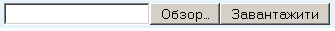
\includegraphics[scale=1,width=8cm]{ch05-01.png}
\caption{Форма завантаження файлу}
\label{f5-1:image}
\end{figure}

Перш, ніж приступити до написання сценарію обробки \verb'multipart'-форми, потрібно відредагувати файл конфігурації \verb'php.ini', щоб дозволити завантаження файлів на сервер.

Конфігураційний файл PHP php.ini має три параметри, пов'язані з завантаженням файлів на сервер:
\begin{enumerate}
\item \verb'file_uploads = On'~--- дозволяє завантаження файлів на сервер по протоколу HTTP;
\item \verb'upoad_tmp_dir = /tmp'~--- встановлює каталог для тимчасового зберігання завантажених файлів;
\item \verb'upload_max_filesize = 2M'~--- встановлює максимальний обсяг завантажуваних файлів. 

\end{enumerate}

Для успішного завантаження та збереження файлу необхідно створити сценарій виду:


\begin{lstlisting}[caption=Завантаження файлу на сервер]
<html>
<head>
  <title> Результат завантаження файлу </title>
</head>
<body>
<?php
if($_FILES["filename"]["size"] > 1024*3*1024)
   {
   echo ("Розмір файлу перевищує три мегабайта");
   exit;
   }
// Перевіряємо	чи	завантажився	файл
if(is_uploaded_file($_FILES["filename"]["tmp_name"]))
   {
   // Якщо так, то переносимо його у кінцевий каталог
   move_uploaded_file($_FILES["filename"]["tmp_name"], 
   "/path/to/file/".$_FILES["filename"]["name"]);
   } 
else 
   {
   echo("Помилка завантаження");
   }
?>
</body></html>
\end{lstlisting}

Слід зауважити, що для доступу до файлу використовується суперглобальний масив \verb'$_FILES', детальний опис якого дано у додатку~\ref{sup-glob:app}.



 
\pagebreak[3]
\section{Індивідуальне завдання}

\nopagebreak[4]
\subsection*{Завдання до лабораторної роботи}
\nopagebreak[4]
\begin{enumerate}
\item Вивчити теоретичний матеріал
\item Відповісти на контрольні запитання
\item Скласти алгоритм (блок-схему) програми
\item Виконати практичне завдання
\item Скласти звіт
\item Захистити роботу
\end{enumerate}

\subsection*{Контрольні запитання}
\nopagebreak[4]
\begin{enumerate}
\item Що таке файл? Що таке каталог?
\item Які основні операції для роботи з файлами ви знаєте?
\item Яким чином можна відкрити/створити файл у РНР?
\item Яким чином проводиться читання з файлу?
\item Яким чином проводиться запис у файл?
\item Яким чином можна переміщувати покажчик у файлі?
\item Що таке блокування файлу?
\item Які види блокування файлів ви знаєте?
\item Які особливості видів блокування файлів?
\item Яким чином завантажити файл на сервер?

\end{enumerate}

\subsection*{Практичні завдання}
\nopagebreak[4]


\begin{enumerate}
\item[]Створити форму з текстовим полем вводу для шляху каталогу та вивести таку інформацію: 
\item список об'єктів каталогу, підкаталоги виділити іншим кольором
\item вивести тільки файли, та реалізувати можливість їх видалення
\item знайти підкаталоги першого рівня та вивести їхній зміст
\item знайти порожні підкаталоги першого рівня, вивести їхні імена та видалити їх
\item створити 10 підкаталогів, та по 10 файлів у кожному, вивести отримане дерево
\item []Написати просту гостьову книгу, що зберігає інформацію у файлах, яка буде записувати та виводити:
\item перші 10 повідомлень користувачів та час відправлення
\item перші 10 повідомлень користувачів та поставлений ними рейтинг від 1 до 10
\item 10 повідомлень з найвищим рейтингом
\item список повідомлень з можливістю їх видалення
\item список повідомлень з можливістю їх редагування
\item[]Продемонструвати роботу гостьової книги 
\item[]Створити книгу рецептів, серед функцій якої є: 
\item виведення рецепту з найвищим рейтингом
\item виведення найсвіжіших рецептів
\item виведення найперших рецептів
\item збереження рецептів в окремих файлах
\item видалення вибраного рецепту
\item редагування вибраного рецепту
\item[]Продемонструвати роботу книги рецептів 
\item[]Створити фотогалерею з функціями додавання фотографії та опису до неї та додатковими функціями: 
\item виведення посилань на фото
\item виведення посилань на опис
\item виведення списку фото та видалення обраного
\item виведення списку та редагування опису обраного
\item обмежити розмір файлу, що завантажується до 1МБ
\item[]Продемонструвати роботу фотогалереї  
\item[]Створити файлове сховище з можливістю завантаження файлу та опису до нього та додатковими функціями:
\item вивести опис файлу та посилання для завантаження
\item реалізувати можливість видалення файлу
\item реалізувати можливість редагування імені файлу
\item реалізувати можливість редагування опису
\item[]Продемонструвати роботу файлового сховища 
\end{enumerate}


%\chapter{Сесії у РНР. Відправлення e-mail}
\section*{Мета роботи}
Навчитися використовувати сесії РНР та cookies. Розібратися в механізмі роботи сесій та cookies. Навчитися використовувати вбудовані засоби відправлення e-mail.
\section{Авторизація доступу}
У сучасних, навіть не дуже складних, веб-системах виникає потреба ідентифікувати користувача та виділити йому окреме поле діяльності. Якщо інформацію про ім'я, пароль та права користувача можна зберігати у файлах або у таблиці бази даних, то залишається проблема стеження за наявністю користувача на сайті.

Цю проблему можна вирішити двома способами:
\begin{itemize}
\item встановленням \verb'cookies'
\item запуском сесії.
\end{itemize}

Механізм сесій налаштований таким чином, що використовує механізм \verb'cookies' для передачі даних, але можливо обходитись і без \verb'cookies' у разі, коли вони відключені у користувача.
\section{Механізм сесії. Налаштування сесії}
\index{PHP!сесії}
\textbf{Сесія}~--- це механізм, який дозволяє створювати і використовувати змінні, зберігають своє значення протягом всього часу роботи користувача з сайтом.

Ці змінні для кожного користувача мають різні значення і можуть використовуватися на будь-якій сторінці сайту до виходу користувача з системи. При цьому кожного разу, заходячи на сайт, користувач отримує нові значення змінних, що дозволяють ідентифікувати його протягом цього сеансу або сесії роботи з сайтом. Звідси й назва механізму~--- сесії. 

Ідентифікатор сесії є 128 бітним числом. Якщо людина прийшла на сайт вперше і PHP-процесор це бачить, то даним відвідувачу присвоюється число, не присвоєне ще нікому. Надалі, при повторному заході, відвідувач буде асоційований з його особистим числом (ідентифікатором), через що програмі буде надана персональна область пам'яті.

Подання ідентифікатору сесії здійснюється у вигляді рядку із 32-х байт. Приклади ідентифікаторів сесії:

\begin{itemize}
\item \verb'7f4cbf53fbcd4717792447f32da7dba8'
\item \verb'ac4f4a45bdc893434c95dcaffb1c1811'
\end{itemize}

Налаштування PHP, в тому числі і для роботи з сесіями, прописуються у файлі \verb'php.ini'. В додатку~\ref{ses-opt:table} та~\ref{ses-opt-full:table} дано базові налаштування механізму сесії.

\subsection*{Унікальність сесій}
Підробити сесію або ідентифікатор не можна. Число з 128 біт (це 2 в 128 ступеня) в десятковому поданні має 38 нулів. Припустимо, на Вашому сайті буде 10~000 відвідувачів. Тоді у хакера шанси кілька зростають до 2 в ступені 114. Але це так само нереальна ймовірність~--- що-небудь підробити. Одна з очевидних причин наступна. Щоб підібрати номер сесії, потрібно зробити запит до Вашого веб-сервера. Нехай кожен запит займає 1024 байти. Через мільярд звернень до Вашого сайту, що складе 1000 ГБ трафіку, явно щось трапиться: Ваш сайт відключать через дикого трафіку або у вас не вистачить грошей на оплату такого великого трафіку. Ваш канал або пропускна здатність провайдера занадто слабка, щоб в розумні терміни перебрати всі номери. Ваш сервер не зможе хоч якось швидко працювати, маючи гігантську кількість пустих файлів, через створення фіктивних сесій. Ваш сервер переповниться лог-файлами і файлами фіктивних сесій, перестане працювати.

\subsection*{Збереження даних сесій}
Є два популярних способи зберігання даних сесій: база даних і файли. Ще можна зберігати сесії в пам'яті сервера (ОЗУ), але при виключенні сервера усі дані будуть втрачені. Зазвичай сесії зберігають у файлах, щоб знизити навантаження на базу даних. У деяких випадках сесії дозволяють повністю відмовитися від бази даних або використовувати її мінімально: в базі даних тільки список логінів/паролів, в сесіях (на файлах) вся робоча інформація.

За замовчуванням PHP зберігає всі в файлах (у своєму форматі) і сам дістає з них збережені дані. Після роботи кожного сценарію PHP сам все записує назад в особистий файл.

\subsection*{Передача ідентифікатора сесії}
Для передачі ідентифікатора сесії існують два основних способи і кілька маловживаних. Розглянемо скорочено механізм їх роботи:

\begin{enumerate}
\item \textbf{Cookies}

Це самий популярний і ефективний спосіб передачі ідентифікатора. Можна один раз помістити в куку змінну і всі інші скрипти будуть її отримувати. Якщо у користувача куки включені, PHP сам помістить туди ідентифікатор і потім сам його звідти дістане. 

Якщо у користувача куки вимкнені, то робота з сайтом може стати неможливою.

\item \textbf{параметри}
\begin{verse}
http://php.spb.ru/test.php?PHPSESSID=ac4f4a45bdc893434c95dcaffb1c1811
\end{verse}

Якщо ви будете дописувати всі ваші посилання подібним чином, то всі ваші наступні скрипти отримають ідентифікатор. PHP використовує і даний метод за замовчуванням (поєднуючи з куками, якщо ті вимкнені). Тобто PHP сам застосує або куки, або отриманий параметр.

Використання такого способу э 100\% надійним, але являється украй небезпечним, т.я. будь-хто може підробити параметр і отримати конфіденціальні дані користувача.

\item \textbf{PathInfo}
\begin{verse}
http://php.spb.ru/test.php/ac4f4a45bdc893434c95dcaffb1c1811
\end{verse}

Це засновано на розумінні веб-сервером того, де з цього URL шлях до скрипта, а де параметри. Тобто Апач розпізнає даний виклик, як звернення до файлу test.php і передасть йому рядок у змінній \verb'$pathinfo = getenv ("PATH_INFO")'. Відповідно, щоб передати управління в інший скрипт, треба подібним чином скласти URL (GET-запит) або передати форму GET або POST запитом.

\item Існують ще методи передачі ідентифікатора сесії, але вони ще менш зручні та не можуть надати надійного захисту від підробки.

\end{enumerate}



\section{Створення сесії, реєстрація змінних сесії, видалення змінних сесії}
\index{PHP!сесії!змінні сесії}
\index{PHP!функції!сесії}
При роботі із сесією виділяють три наступні етапи:
\begin{enumerate}
\item відкриття сесії
\item реєстрація змінних та їх використання
\item закриття сесії
\end{enumerate}
Нижче буде розглянуто всі три етапи.

\subsection*{Створення сесії}
Перше, що потрібно зробити для роботи з сесіями (якщо вони вже налаштовані адміністратором сервера), це запустити механізм сесій. Якщо в налаштуваннях сервера змінна \verb'session.auto_start = 0' (якщо \verb'session.auto_start = 1', то сесії запускаються автоматично), то будь-який скрипт, в якому потрібно використовувати дані сесії, повинен починатися з команди
\begin{verbatim}
  session_start(); 
\end{verbatim}

Отримавши таку команду, сервер створює нову сесію або відновлює поточну, ґрунтуючись на ідентифікаторі сесії, переданому за запитом.  Інтерпретатор PHP шукає змінну, в якій зберігається ідентифікатор сесії (за замовчуванням це \verb'PHPSESSID') спочатку в \verb'cookies', потім у змінних, переданих за допомогою \verb'POST' і \verb'GET'-запитів. Якщо ідентифікатор знайдений, то користувач вважається ідентифікованим, проводиться заміна всіх URL і виставляння \verb'cookies'. В іншому випадку користувач вважається новим, для нього генерується новий унікальний ідентифікатор, потім проводиться заміна URL і виставляння \verb'cookies'.

Нижче дано приклад роботи сесії:

\begin{verbatim}
<?
session_start(); 
echo session_id(); 
?>
<html>
<head><title>My home page</title></head>
... // домашняя страничка
</html>
<?
echo session_name(); 
?>
\end{verbatim}

Якщо оновити таку сторінку, то буде видно, що рядок, котрий друкує \verb'echo session_id();', не змінюється. Це вказує на те, що оновлення сесії проводиться успішно. Якщо закрити вікно браузера та відкрити цю сторінку знову, \verb'echo session_id();' видасть нове значення, томущо \verb'cookies' з минулої сесії вже знищено.


\subsection*{Реєстрація змінних}
Однак від самих ідентифікатора та імені сесії нам користі для вирішення завдань небагато. На практиці необхідно передавати щонайменше логін та пароль користувача. Для того щоб цього досягти, потрібно просто зареєструвати свої змінні:
\begin{verbatim}
session_register (ім'я_змінної1, 
        ім'я_змінної2, ...); 
\end{verbatim}
Зауважимо, що реєструються не значення, а імена змінних. Зареєструвати змінну досить один раз на будь-якій сторінці, де використовуються сесії. Імена змінних передаються функції \verb'session_register()' без знака <<\$>>. Всі зареєстровані таким чином змінні стають глобальними протягом даної сесії роботи з сайтом. 



\subsection*{Видалення змінних, сесії}
Крім вміння реєструвати змінні сесії (тобто робити їх глобальними протягом усього сеансу роботи), корисно також вміти видаляти такі змінні і сесію в цілому.

Функція \verb|session_unregister(ім'я_змінної)| видаляє глобальну змінну з поточної сесії (тобто видаляє її зі списку зареєстрованих змінних). Якщо реєстрація проводилася за допомогою \verb'$_SESSION', то використовують мовну конструкцію \verb'unset()'. Вона не повертає ніякого значення, а просто знищує зазначені змінні. Для того щоб скинути значення всіх змінних сесії, можна використовувати функцію \verb'session_unset();'.

Знищити поточну сесію цілком можна командою \verb'session_destroy();'. Вона не скидає значення глобальних змінних сесії і не видаляє \verb'cookies', а знищує всі дані, асоційовані з поточною сесією.

Перелік згаданих вище функцій дано у додатку~\ref{ses-func:text}. 
\section{Робота з cookies}
\index{PHP!cookies}

\textbf{Cookies}~--- це механізм зберігання даних браузером віддаленого комп'ютера для ідентифікації відвідувачів, що повертаються, та зберігання параметрів веб-сторінок (наприклад, змінних).

\textbf{Cookies}~--- це текстові рядки, що зберігаються на стороні клієнта, і містять пари <<ім'я-значення>>, з якими пов'язаний URL, по якому браузер визначає чи потрібно посилати \verb'cookies' на сервер.

Етапи роботи з  \verb'cookies' схожі на етапи використання механізму сесій:
\begin{enumerate}
\item встановлення \verb'cookies'
\item використання \verb'cookies'
\item видалення \verb'cookies'
\end{enumerate}
\subsection*{Встановлення cookies}
Встановлення cookies проводиться за допомогою функції \verb'setcookie()'. Ця функція має такі аргументи:
\begin{itemize}
\item \verb'name'~--- ім'я встановлюваного cookie;
\item \verb'value'~--- значення, яке зберігається в \verb'cookie' з ім'ям name;
\item \verb'expire'~--- час в секундах з початку епохи, по витікання якого поточний \verb'cookie' стає недійсним;
\item \verb'path'~--- шлях, по якому доступний cookie;
\item \verb'domain'~--- домен, з якого доступний cookie;
\item \verb'secure'~--- директива, яка визначає, чи доступний \verb'cookie' не по запиту HTPPS. За замовчуванням ця директива має значення 0, що означає можливість доступу до \verb'cookie' по звичайному запитом HTTP. 
\end{itemize}

При використанні Cookies необхідно мати на увазі, що Cookies повинні встановлюватися до першого виводу інформації в браузер (наприклад, оперетором echo або висновком якої функції). Тому бажано встановлювати Cookies на самому початку скрипта. Cookies встановлюються за допомогою певного заголовка сервера, а якщо скрипт виводить небудь, то це означає, що починається тіло документа. В результаті Cookies не будуть встановлені і може бути виведено попередження. Для перевірки успішності установки Cookies можна використовувати такий метод:

\begin{verbatim}
<?php
if (SetCookie("Test","Value")) 
echo "<h3>Cookies успішно встановлено!</h3>";
?>
\end{verbatim}

Функція \verb'SetCookie()' повертає TRUE у разі успішного встановлення Cookie. У разі, якщо Cookie встановити не вдається \verb'SetCookie()' поверне FALSE і можливо, попередження (залежить від налаштувань PHP). 


\subsection*{Використання cookies}

Доступ до \verb'cookie' здійснюється через суперглобальний масив \verb'$_COOKIE["name"]', де <<name>>~--- ім'я параметру, значення котрого необхідно отримати.

При читанні значень Cookies звертайте увагу на перевірку існування Cookies, наприклад, використовуючи оператор \verb'isset()'. Або шляхом придушення виведення помилок опереатором <<@>>.

Приклад встановлення Cookie і подальшого його читання:
\begin{verbatim}
<? php
setcookie( "test" , "Hello" , time()+3600 );
echo @$_COOKIE['test'];
?>
\end{verbatim}

У прикладі нижче показано як створити лічильник завантажень сторінки:
\begin{lstlisting}[caption=Лічильник завантажень сторінки]
<?php
// Проверяем, был ли уже установлен Cookie 'Mortal',
// Если да, то читаем его значение,
// И увеличиваем значение счетчика обращений к странице:
if (isset($_COOKIE['Mortal'])) $cnt=$_COOKIE['Mortal']+1;
else $cnt=0;
// Устанавливаем Cookie 'Mortal' зо значением счетчика,
// С временем "жизни" до 18/07/29,
// То есть на очень долгое время:
setcookie("Mortal",$cnt,0x6FFFFFFF);
// Выводит число посещений (загрузок) этой страницы:
echo "<p>Вы посещали эту страницу <b>".@$_COOKIE['Mortal']."</b> раз</p>";
?>
\end{lstlisting}

\subsection*{Встановлення масиву cookies}

Ми може встановити масив Cookies, використовуючи квадратні дужки в іменах Cookies \verb'[]', а потім прочитати масив Cookies і значення цього масиву:

\begin{lstlisting}[caption=Масив Cookies]
 <? php
// Устанавливаем массив Cookies:
setcookie("cookie[1]","Первый");
setcookie("cookie[2]","Второй");
setcookie("cookie[3]","Третий");
// После перезагрузки страницы мы отобразим
// Состав массива Cookies 'cookie':
if (isset($_COOKIE['cookie']))   
{
foreach ($_COOKIE ['cookie'] as $name => $value )   
   {
   echo "$name : $value <br>";
   }
}
?> 
\end{lstlisting}

\subsection*{Видалення cookies}

Іноді виникає необхідність видалення Cookies. Зробити це нескладно, необхідно лише знову встановити Cookie з ідентичним ім'ям і порожнім параметром. Наприклад:
\begin{verbatim}
<? php
SetCookie("Test" , "" );
?> 
\end{verbatim}


\section{Відправлення e-mail}
\index{PHP!функції!mail()}
\index{PHP!e-mail}
Найпростіший спосіб відправити лист за допомогою PHP~--- скористатися стандартною функцією \verb'mail()'. Вона має наступний синтаксис:
\begin{verbatim}
bool mail(to, subject, message [, additional\_headers 
[, additional\_parameters]])
\end{verbatim}

Обов'язкові параметри:
\begin{itemize}
\item E-mail одержувача
\item Заголовок листа
\item Текст листа 
\end{itemize}

Необов'язкові параметри:
\begin{itemize}
\item Додаткові заголовки листи
\item Додаткові параметри командного рядка 
\end{itemize}
Повертає значення:
\begin{itemize}
\item true, якщо лист було прийнято до доставки
\item false, в іншому випадку. 
\end{itemize}
Найпростіший приклад її використання виглядає так:
\begin{verbatim}
<?php
mail("joecool@example.com" , "My Subject" , "Line 1\nLine 2\nLine 3" );
?>
\end{verbatim}
Якщо у Вас на екрані з'явилася помилка <<Fatal error: Call to undefined function: mail()>>, це означає, що або PHP зібраний без підтримки функції mail, або вона заборонена налаштуваннями сервера. Така практика останнім часом широко поширена на безкоштовних хостингових серверах. Якщо Ви зіткнулися з такою проблемою, скористайтеся можливістю відправки листів за допомогою сокетів (sockets). 


\section{Альтернатива <<mail()>>}
\index{Системні додатки!sendmail}
На сьогоднішній день поширені наступні способи відправки листів з php-скриптів:
\begin{enumerate}
\item За допомогою виклику функції mail
\item Безпосередньо викликом sendmail
\item За допомогою сокетів
\item Використовуючи COM-об'єкт 
\end{enumerate}
\subsection*{sendmail}
\begin{lstlisting}[caption=Використання sendmail]
<?php
$sendmail = "/usr/sbin/sendmail -t -f $sender -C /etc/sendmail.orig.cf";
$fd = popen($sendmail, "w");
fputs($fd, "To: recipient@example.com\r\n");
fputs($fd, "From: \"Sender Name\" <$sender>\r\n");
fputs($fd, "Subject: Finally\r\n");
fputs($fd, "X-Mailer: Mailer Name\r\n\r\n");
fputs($fd, $body);
pclose($fd);
?> 
\end{lstlisting}
\subsection*{Active-X (COM)}
\begin{lstlisting}[caption=Використання Active-X]
<?php
@$CDONTS = new COM("CDONTS.NewMail");

@$CDONTS->From = "from_user@domain.com";
@$CDONTS->To = "to_user@domain.com";
@$CDONTS->CC = "cc_user@domain.com";
@$CDONTS->BCC = "bcc_user@domain.com";

@$CDONTS->BodyFormat = 0;
@$CDONTS->MailFormat = 0;

//@$CDONTS->AttachFile("c:\file.txt");

@$CDONTS->Subject = "Using CDONTS with PHP4 and IIS";
@$CDONTS->Body = "Blah blah blah blah, bleh...";

@$CDONTS->Send();
@$CDONTS->Close();
?> 
\end{lstlisting}

У разі роботи з сокетом відправлення дещо ускладнюється. Роботу з сокетами буде розглянуто в наступних лабораторних роботах.

\pagebreak[3]
\section{Індивідуальне завдання}

\nopagebreak[4]
\subsection*{Завдання до лабораторної роботи}
\nopagebreak[4]
\begin{enumerate}
\item Вивчити теоретичний матеріал
\item Відповісти на контрольні запитання
\item Скласти алгоритм (блок-схему) програми
\item Виконати практичне завдання
\item Скласти звіт
\item Захистити роботу
\end{enumerate}

\subsection*{Контрольні запитання}
\nopagebreak[4]
\begin{enumerate}
\item Що таке сесії? Для чого вони потрібні?
\item Яким чином забезпечується унікальність сесій?
\item Де зберігаються дані сесії?
\item Як створити сесію? 
\item Яким чином додати та видалити змінну сесії?
\item Що таке cookies?
\item Як використовувати cookies?
\item Як створити та використати масив cookies?
\item Яким чином можна відправити електронний лист?
\item Які альтернативи відправлень електронних листів ви знаєте?
\end{enumerate}

\subsection*{Практичні завдання}
\nopagebreak[4]


\begin{enumerate}
\item[]Написати HTML-сторінку з полями вводу логіну та паролю та додати наступний функціонал:
\item створити гостьову книгу, що зберігає запис користувача, виводить його записи, та дозволяє додавати нові без повторної авторизації
\item створити гостьову книгу що виводить перелік повідомлень та дозволяє видаляти їх певному користувачу без повторної авторизації
\item створити книгу рецептів, що дозволяє додавати, та дивитись додані рецепти тільки власнику записів послідовно без повторної авторизації
\item створити книгу рецептів, що дозволяє одному користувачу додавати рецепти, а іншому~--- видаляти
\item створити фотогалерею, що дозволяє додавати зображення та виводити їх перелік без повторної авторизації
\item створити фотогалерею, що дозволяє додавати зображення та видаляти їх певному користувачу без повторної авторизації
\item створити декілька зв'язаних сторінок, для різних користувачів виводити різну інформацію
\item створити примітивний форум на кілька користувачів (авторизація, додавання повідомлення, виведення повідомлень та імен користувачів)
\item створити сайт зі статтями, дати можливість просмотру неавторизованим користувачам та додавання авторизованим
\item створити сайт за статтями, дати можливість певним користувачам видаляти їх, заборонити просмотр неавторизованим користувачам
\item створити примітивний форум на кілька користувачів (авторизація, додавання повідомлення, виведення повідомлень та імен користувачів), що працює виключно на cookies
\item створити гостьову книгу, що зберігає запис користувача, виводить його записи, та дозволяє додавати нові без повторної авторизації, книга працює виключно на cookies
\item створити книгу рецептів, що дозволяє одному користувачу додавати рецепти, а іншому~--- видаляти, книга працює виключно на cookies
\item створити фотогалерею, що дозволяє додавати зображення та виводити їх перелік без повторної авторизації, фотогалерею працює виключно на cookies
\item створити примітивний онлайн-щоденник (додавання записів, виведення списку записів)
\item створити примітивний онлайн-щоденник (додавання записів, виведення списку записів), авторизацію користувача проводити за допомогою cookies
\item створити простий калькулятор (<<+>>, <<->>, <<*>>, <</>>) та виводити історію користувацьких обчислень 
\item створити простий калькулятор (<<+>>, <<->>, <<*>>, <</>>) та виводити історію користувацьких обчислень, авторизацію користувача проводити за допомогою cookies
\item створити гостьову книгу що виводить перелік повідомлень та дозволяє видаляти їх певному користувачу без повторної авторизації, авторизацію користувача проводити за допомогою cookies
\item створити простий калькулятор (<<+>>, <<->>, <<*>>, <</>>), записувати історію обчислень та виводити її адміністратору сайту
\item створити сторінку, що виводить адміністратору логін та пароль користувачів, та дозволяє їх змінювати 
\item створити сторінку, що виводить адміністратору логін та привілеї користувача, та дає право надавати права адміністратора
\item створити сторінку, яка дозволяє адміністратору видаляти користувачів з системи
\item створити сторінку, яка дозволяє додавати користувачів в систему
\item  створити фотогалерею, що дозволяє додавати зображення та видаляти їх певному користувачу без повторної авторизації, авторизацію користувача проводити за допомогою cookies
\item[]Результати роботи виводити у браузері.

\end{enumerate}



\chapter{Взаємодія РНР з СКБД MySQL}
\section*{Мета роботи}
Навчитися працювати з СУБД MySQL, записувати та отримувати табличні дані. Опрацювати взаємодію мови РНР з СУБД MySQL.

\section{Мова запитів SQL, та типи даних у СУБД MySQL}
\index{MySQL!SQL}
\subsection*{Основні команди}
Команди SQL можна поділити на дві категорії:
\begin{itemize}
\item команди означення даних
\item команди обробки даних
\end{itemize}

Перша категорія команд відповідає за створення або видалення баз даних, таблиць баз даних, редагування структури таблиць та типів даних полів таблиць.
До цієї категорії належать наступні команди:

\begin{itemize}
\item CREATE
\item DROP
\item ALTER
\item RENAME
\end{itemize}

Друга категорія команд відповідає за внесення даних до таблиць, оновлення та видалення даних.
До цієї категорії належать наступні команди:

\begin{itemize}
\item SELECT
\item INSERT
\item DELETE
\item UPDATE
\item HANDLER
\item TRUNCATE
\item REPLACE
\item LOAD DATA INFILE
\item DO
\end{itemize}

Нижче більш детально розглянуто синтаксис команд.

\subsection*{Команди означення даних}
\subsubsection*{CREATE}
\index{MySQL!SQL!CREATE}
Для створення бази даних необхідно використати наступну послідовність команд:

\begin{verbatim}
CREATE DATABASE [IF NOT EXISTS] db_name
\end{verbatim}

Оператор \verb'CREATE DATABASE' створює базу даних з вказаним іменем. Якщо база даних вже існує і не зазначений ключовий параметр \verb'IF NOT EXISTS', то виникає помилка виконання команди. 

Скорочений вид синтаксису команди створення таблиці виглядає наступним чином:

\begin{verbatim}
 CREATE [TEMPORARY] TABLE [IF NOT EXISTS] 
 tbl_name [(create_definition, ...)]
 [Table_options] [select_statement]
\end{verbatim}

Оператор створює таблицю. Якщо таблиця вже існує і не зазначений параметр \verb'IF NOT EXISTS', то виникає помилка виконання команди. Параметри таблиці та перелік полів вказують після означення імені таблиці. Приклад створення таблиці надано нижче:
\begin{verbatim}
 CREATE TABLE table123 (f1 INT, f2 INT)
\end{verbatim}
Створюється таблиця з двома полями цілочисельного типу.

Повний перелік можливих параметрів команди дано у додатку~\ref{crtab:text}.

Для створення індексів у СУБД MySQL існує команда CREATE INDEX. Синтаксис команди надано нижче: 
\begin{verbatim}
 CREATE [UNIQUE | FULLTEXT] INDEX index_name
         ON tbl_name (col_name [(length)], ...)
\end{verbatim}
Команда CREATE INDEX у версіях MySQL до 3.22 не виконує ніяких дій. У версії 3.22 і більш пізніх CREATE INDEX відповідає команді ALTER TABLE в частині створення індексів. Зазвичай всі індекси створюються в таблиці під час створення самої таблиці командою CREATE TABLE. CREATE INDEX дає можливість додати індекси до існуючих таблиць.


\subsubsection*{DROP}
\index{MySQL!SQL!DROP}
Для видалення бази даних існує наступна команда:
\begin{verbatim}
 DROP DATABASE [IF EXISTS] db_name
\end{verbatim}
Оператор DROP DATABASE видаляє всі таблиці в зазначеній базі даних і саму базу. Якщо ви виконуєте DROP DATABASE на базі даних, символічно пов'язаної з іншою, то видаляється як посилання, так і оригінальна база даних. Будьте дуже уважні при роботі з цією командою!

Оператор DROP DATABASE повертає кількість файлів, які були видалені з директорії бази даних. Як правило, це число дорівнює кількості таблиць, помноженому на три, оскільки зазвичай кожна таблиця представлена трьома файлами: .MYD-файлом, MYI-файлом і .Frm-файлом.

Команда DROP DATABASE видаляє з директорії зазначеної бази даних всі файли з наступними розширеннями: <<.BAK>>, <<.DAT>>, <<.HSH>>, <<.ISD>>, <<.ISM>>, <<.ISM>>, <<.MRG>>, <<.MYD>>, <<.MYI>>, <<.Db>>, <<.Frm>>. 	

Всі піддиректорії, імена яких складаються з двох цифр (RAID-директорії), також видаляються.

У версії MySQL 3.22 і більш пізніх можна використовувати ключові слова IF EXISTS для попередження помилки, якщо зазначена база даних не існує. 

Щоб видалити таблицю з поточної бази даних необхідно виконати наступну команду: 
\begin{verbatim}
 DROP TABLE [IF EXISTS] tbl_name 
 [, tbl_name, ...] [RESTRICT | CASCADE]
\end{verbatim}
Оператор DROP TABLE видаляє одну або декілька таблиць. Всі табличні дані та визначення видаляються, так що будьте уважні при роботі з цією командою!

У версії MySQL 3.22 і більш пізніх можна використовувати ключові слова IF EXISTS , щоб попередити помилку, якщо зазначені таблиці не існують. 

Для видалення індексів з таблиць необхідно використати команду
\begin{verbatim}
 DROP INDEX index_name ON tbl_name
\end{verbatim}
Оператор DROP INDEX видаляє індекси, зазначені в index\_name з таблиці tbl\_name. DROP INDEX не виконує ніяких дій у версіях MySQL до 3.22. У версіях 3.22 і більш пізніх DROP INDEX відповідає команді ALTER TABLE в частині видалення індексів.
\subsubsection*{ALTER}
\index{MySQL!SQL!ALTER}
Скорочений синтаксис команди для зміни структури таблиць виглядає наступним чином:
\begin{verbatim}
 ALTER [IGNORE] TABLE tbl_name alter_spec 
 [, alter_spec ...]
\end{verbatim}
Оператор ALTER TABLE забезпечує можливість змінювати структуру існуючої таблиці. Наприклад, можна додавати або видаляти стовпці, створювати або знищувати індекси або перейменовувати стовпці або саму таблицю. Можна також змінювати коментар для таблиці та її тип.

Нижче надано приклади використання команди:

Для того щоб змінити тип стовпця з INTEGER на TINYINT NOT NULL (залишаючи ім'я колишнім) і змінити тип стовпця b з CHAR(10) на CHAR(20) з перейменуванням його з b на c :
\begin{verbatim}
ALTER TABLE t2 MODIFY a TINYINT NOT NULL, 
      CHANGE bc CHAR (20);
\end{verbatim}

Для того щоб додати індекс до стовпцю d і зробити стовпець a первинним ключем:
\begin{verbatim}
ALTER TABLE t2 ADD INDEX (d), ADD PRIMARY KEY (a);
\end{verbatim}

Повні дані щодо синтаксису ALTER TABLE дано в додатку~\ref{alttab:text}.

\subsubsection*{RENAME}
\index{MySQL!SQL!RENAME}
Для перейменування таблиць, починаючи з версії 3.22, введено команду RENAME TABLE.
\begin{verbatim}
 RENAME TABLE tbl_name TO new_tbl_name 
 [, tbl_name2 TO new_tbl_name2, ...]
\end{verbatim}
Операція перейменування повинна здійснюватися як атомарна, тобто при виконанні перейменування ніякому іншому потоку не дозволяється доступ до зазначених таблиць. Завдяки цьому можливе заміщення таблиці порожній таблицею:
\begin{verbatim}
 CREATE TABLE new_table (...);
 RENAME TABLE old_table TO backup_table, 
 new_table TO old_table;
\end{verbatim}
Перейменування проводиться зліва направо. Таким чином, для обміну іменами між двома таблицями необхідно виконати наступні дії:
\begin{verbatim}
 RENAME TABLE old_table TO backup_table,
         new_table TO old_table,
         backup_table TO new_table;
\end{verbatim}
Для двох баз даних, що знаходяться на одному і тому ж диску, можна також здійснювати обмін іменами:
\begin{verbatim}
 RENAME TABLE current_db.tbl_name 
 TO other_db.tbl_name;
\end{verbatim}
При виконанні команди RENAME не повинні мати місце заблоковані таблиці або активні транзакції. Необхідно також мати привілеї ALTER і DROP для початкової таблиці і привілеї CREATE і INSERT~--- для нової.

Якщо MySQL стикається з якою-небудь помилкою при перейменуванні декількох таблиць, то станеться зворотне перейменування для всіх перейменованих таблиць, щоб повернути все в початковий стан. 

\subsection*{Команди обробки даних}
\subsubsection*{SELECT}
\index{MySQL!SQL!SELECT}

Оператор SELECT має наступну структуру:
\begin{verbatim}
 SELECT [STRAIGHT_JOIN]
        [SQL_SMALL_RESULT] [SQL_BIG_RESULT] 
        [SQL_BUFFER_RESULT] [SQL_CACHE | SQL_NO_CACHE] 
        [SQL_CALC_FOUND_ROWS] [HIGH_PRIORITY]
        [DISTINCT | DISTINCTROW | ALL]
     select_expression, ...
     [INTO {OUTFILE | DUMPFILE} 
     'file_name' export_options]
     [FROM table_references
       [WHERE where_definition]
       [GROUP BY {unsigned_integer | 
       col_name | formula} [ASC | DESC], ...]
       [HAVING where_definition]
       [ORDER BY {unsigned_integer | 
       col_name | formula} [ASC | DESC], ...]
       [LIMIT [offset,] rows]
       [PROCEDURE procedure_name]
       [FOR UPDATE | LOCK IN SHARE MODE]]
\end{verbatim}
SELECT застосовується для вилучення рядків, вибраних з однієї або декількох таблиць. Вираз select\_expression задає стовпці, в яких необхідно проводити вибірку. Крім того, оператор SELECT можна використовувати для витягання рядків, обчислених без посилання якусь таблицю. Наприклад запит \verb'SELECT 1 + 1;' поверне значення <<2>>.

\subsubsection*{INSERT}
\index{MySQL!SQL!INSERT}
\begin{verbatim}
     INSERT [LOW_PRIORITY | DELAYED] 
         [IGNORE] [INTO] tbl_name [(col_name, ...)]
         VALUES (expression, ...), (...), ...
 або INSERT [LOW_PRIORITY | DELAYED] [IGNORE]
         [INTO] tbl_name [(col_name, ...)]
         SELECT ...
 або INSERT [LOW_PRIORITY | DELAYED] [IGNORE]
         [INTO] tbl_name
         SET col_name = expression, 
         col_name = expression, ...
\end{verbatim}
Оператор INSERT вставляє нові рядки в існуючу таблицю. Форма даної команди INSERT \dots VALUES вставляє рядки відповідно до точно зазначеними в команді значеннями. Форма INSERT \dots SELECT вставляє рядки, обрані з іншої таблиці або таблиць. Форма INSERT ... VALUES зі списком з декількох значень підтримується у версії MySQL 3.22.5 і більш пізніх. Синтаксис вираження col\_name=expression підтримується у версії MySQL 3.22.10 і більш пізніх. 

Команда INSERT \dots SELECT забезпечує можливість швидкого внесення великої кількості рядків у таблицю з однієї або більше таблиць.
\begin{verbatim}
 INSERT INTO tblTemp2 (fldID) 
         SELECT tblTemp1.fldOrder_ID 
         FROM tblTemp1
         WHERE tblTemp1.fldOrder_ID > 100;
\end{verbatim}

\subsubsection*{DELETE}
\index{MySQL!SQL!DELETE}
\begin{verbatim}
DELETE [LOW_PRIORITY | QUICK] FROM table_name
       [WHERE where_definition]
       [ORDER BY ...]
       [LIMIT rows]

или

DELETE [LOW_PRIORITY | QUICK] table_name[.*] [,table_name[.*] ...]
       FROM table-references
       [WHERE where_definition]

oили

DELETE [LOW_PRIORITY | QUICK]
       FROM table_name[.*], [table_name[.*] ...]
       USING table-references
       [WHERE where_definition]
\end{verbatim}
Оператор DELETE видаляє з таблиці table\_name рядки, що задовольняють заданим в where\_definition умовам, і повертає число віддалених записів.

Якщо оператор DELETE запускається без визначення WHERE, то видаляються всі рядки. При роботі в режимі AUTOCOMMIT це буде аналогічно використанню оператора TRUNCATE. В MySQL 3.23 оператор DELETE без визначення WHERE поверне нуль як число віддалених записів.
\subsubsection*{UPDATE}
\index{MySQL!SQL!UPDATE}

\begin{verbatim}
UPDATE [LOW_PRIORITY] [IGNORE] tbl_name
    SET col_name1=expr1 [, col_name2=expr2, ...]
    [WHERE where_definition]
    [LIMIT #]
\end{verbatim}
Оператор UPDATE оновлює стовпці відповідно до їх новими значеннями в рядках існуючої таблиці. У виразі SET вказується, які саме стовпці слід модифікувати і які величини повинні бути в них встановлені. У виразі WHERE, якщо воно присутнє, задається, які рядки підлягають оновленню. В інших випадках оновлюються всі рядки. Якщо задано вираз ORDER BY, то рядки будуть оновлюватися у зазначеному в ньому порядку.

Якщо вказується ключове слово LOW\_PRIORITY, то виконання даної команди UPDATE затримується до тих пір, поки інші клієнти не завершать читання цієї таблиці.

Якщо вказується ключове слово IGNORE, то команда оновлення не буде перервана, навіть якщо при оновленні виникне помилка дублювання ключів. Рядки, через які виникають конфліктні ситуації, оновлені не будуть.

Якщо доступ до стовпцю із зазначеного виразу здійснюється по аргументу tbl\_name, то команда UPDATE використовує для цього стовпця його поточне значення.
\subsubsection*{HANDLER}
\index{MySQL!SQL!HANDLER}
Оператор HANDLER забезпечує прямий доступ до інтерфейсу дескриптора таблиці MyISAM, минаючи оптимізатор SQL. Отже, цей оператор працює швидше, ніж SELECT.

Перша форма оператора HANDLER відкриває таблицю, роблячи її доступною для послідовності команд HANDLER \dots READ. Цей об'єкт недоступний іншим потокам і не буде закритий, поки даний потік не викличе HANDLER tbl\_name CLOSE або сам потік не буде знищений.

Друга форма вибирає один рядок (або більше - у відповідності з установкою в вираженні LIMIT), для якої (их) зазначений індекс відповідає заданій умові і умова в виразі WHERE також виконується. Якщо індекс складається з декількох частин (охоплює декілька стовпців), то складові його величини вказуються у вигляді розділеного комами списку. Забезпечуються величини тільки для декількох перших шпальт.

Третя форма вибирає один рядок (або більше - у відповідності з установкою в вираженні LIMIT), з таблиці; гаразд вказівки індексів у відповідності з умовою WHERE.

Четверта форма (без зазначення індексів) вибирає один рядок (або більше - у відповідності з установкою в вираженні LIMIT), з таблиці, використовуючи природний порядок рядків (як вони зберігаються у файлі даних), у відповідності з умовою WHERE. Ця форма працює швидше, ніж HANDLER tbl\_name READ index\_name, в тих випадках, коли бажаний перегляд всієї таблиці.

Оператор HANDLER \dots CLOSE закриває таблицю, відкриту оператором HANDLER ... OPEN.
\subsubsection*{TRUNCATE}
\index{MySQL!SQL!TRUNCATE}
\begin{verbatim}
TRUNCATE TABLE table_name
\end{verbatim}
TRUNCATE TABLE має наступні відмінності від DELETE FROM ...:
\begin{itemize}
\item Ця операція видаляє і відтворює таблицю, що набагато швидше, ніж почергове видалення рядків.
\item Операція є нетранзакціонной; якщо одночасно виконується транзакція або активна блокування таблиці, то можна отримати помилку.
\item Не повертає кількість вилучених рядків.
\item Поки існує коректний файл <<table\_name.frm>>, таблицю можна відтворити з його допомогою, навіть якщо файли даних або індексів пошкоджені.
\end{itemize}

TRUNCATE є розширенням Oracle SQL.
\subsubsection*{REPLACE}
\index{MySQL!SQL!REPLACE}
\begin{verbatim}
    REPLACE [LOW_PRIORITY | DELAYED]
        [INTO] tbl_name [(col_name,...)]
        VALUES (expression,...),(...),...
или REPLACE [LOW_PRIORITY | DELAYED]
        [INTO] tbl_name [(col_name,...)]
        SELECT ...
или REPLACE [LOW_PRIORITY | DELAYED]
        [INTO] tbl_name
        SET col_name=expression, col_name=expression,...
\end{verbatim}

Оператор REPLACE працює точно так само, як INSERT, за винятком того, що якщо стара запис у даній таблиці має те ж значення індексу UNIQUE або PRIMARY KEY, що і нова, то стара запис перед занесенням нової буде видалена.

\subsubsection*{LOAD DATA INFILE}
\index{MySQL!SQL!LOAD DATA INFILE}

\begin{verbatim}
LOAD DATA [LOW_PRIORITY | CONCURRENT] [LOCAL] INFILE 'file_name.txt'
    [REPLACE | IGNORE]
    INTO TABLE tbl_name
    [FIELDS
        [TERMINATED BY '\t']
        [[OPTIONALLY] ENCLOSED BY '']
        [ESCAPED BY '\\' ]
    ]
    [LINES TERMINATED BY '\n']
    [IGNORE number LINES]
    [(col_name,...)]
\end{verbatim}

Команда LOAD DATA INFILE читає рядки з текстового файлу і вставляє їх у таблицю з дуже високою швидкістю. Якщо задано ключове слово LOCAL, то файл читається з клієнтського хоста. Якщо ж LOCAL не вказується, то файл повинен знаходитися на сервері. (Опція LOCAL доступна у версії MySQL 3.22.6 і більш пізніх.)

Якщо текстові файли, які потрібно прочитати, знаходяться на сервері, то з міркувань безпеки ці файли повинні або розміщуватися в директорії бази даних, або бути доступними для читання всім користувачам. Крім того, для застосування команди LOAD DATA INFILE до серверних файлів необхідно володіти привілеями FILE для серверного хосту.


\subsubsection*{DO}
\index{MySQL!SQL!DO}

\begin{verbatim}
DO expression, [expression, ...]
\end{verbatim}
Виконує даний вираз, але не повертає небудь результат. Є скороченою формою оператора SELECT expression, expression, але перевага його полягає в тому, що він працює трохи швидше, якщо немає необхідності в поверненні результату.

Оператор головним чином корисний при використанні з функціями, які мають побічні ефекти, такими як RELEASE\_LOCK.
\section{Функції для роботи з MySQL. Виконання SQL-запитів}
\index{MySQL!PHP!функції}

\section{Установка з'єднання. Вибір бази даних}
\index{MySQL!таблиці}

\section{Вибірка з таблиці, розбір результату вибірки}
\index{MySQL!вибірка}

\section{Додавання записів, оновлення записів}
\index{MySQL!додавання}
\index{MySQL!оновлення}
\section{Очищення і видалення таблиць}
\index{MySQL!очищення таблиць}
\index{MySQL!видалення таблиць}
\pagebreak[3]
\section{Індивідуальне завдання}

\nopagebreak[4]
\subsection*{Завдання до лабораторної роботи}
\nopagebreak[4]
\begin{enumerate}
\item Вивчити теоретичний матеріал
\item Відповісти на контрольні запитання
\item Скласти алгоритм (блок-схему) програми
\item Виконати практичне завдання
\item Скласти звіт
\item Захистити роботу
\end{enumerate}

\subsection*{Контрольні запитання}
\nopagebreak[4]
\begin{enumerate}
\item Що таке рядки?
\item Яким чином можна задати рядковий літерал?
\item Яка особливість рядків у подвійних лапках?
\item Яка особливість синтаксису \verb'Heredoc'? 
\item Яким чином вивести HTML-код на веб-сторінці?
\item Що таке регулярні вирази?
\item Яка особливість метасимволу <<\verb'\'>>?
\item Для чого використвуються регулярні вирази?
\item Які функції для роботи з регулярними виразами ви знаєте?
\item Яким чином можна використовувати регулярні вирази в SQL-запитах?
\end{enumerate}

\subsection*{Практичні завдання}
\nopagebreak[4]


\begin{enumerate}
\item[]Написати HTML-сторінку з формою, що складається з:
\item однорядкового поля вводу, поля вводу пароля та кнопки відправлення форми.
\item 

\end{enumerate}


\chapter{ООП. Робота з XML}
\index{PHP!ООП}
Хоча РНР володіє загальними об'єктно-орієнтованими можливостями, він не є повноцінною ОО-мовою (наприклад, такою, як C++ або Java). Зокрема, в РНР не підтримуються наступні об'єктно-орієнтовані можливості:
\begin{itemize}
\item множинне спадкування;
\item автоматичний виклик конструкторів (якщо ви хочете, щоб при конструюванні об'єкта похідного класу викликався конструктор базового класу, вам доведеться викликати його явно);
\item абстрактні класи;
\item перевантаження методів;
\item перевантаження операторів (це пов'язано з тим, що РНР є мовою з вільною типізацією);
закритий і відкритий доступ, віртуальні функції;
\item деструктори.
\end{itemize}

Але і без усього перерахованого ви все одно зможете отримати користь з об'єктно-орієнтованих можливостей, підтримуваних РНР. Реалізація ООП в РНР надає колосальну допомогу в модульному оформленні функціональності вашої програми.
\section{Класи та об'єкти. Методи}
\index{PHP!ООП!класи}
\index{PHP!ООП!об'єкти}
Класи утворюють синтаксичну базу об'єктно-орієнтованого програмування. Їх можна розглядати як свого роду <<контейнери>> для логічно пов'язаних даних і функцій (методів). Клас являє собою шаблон, по якому створюються конкретні екземпляри, використовуються в програмі. Екземпляри класів називаються об'єктами.

\subsection{Оголошення класу}
Клас можна розглядати як тип даних, а об'єкт~--- як змінну. Програма може одночасно працювати з декількома об'єктами одного класу як і з декількома змінними. Загальний формат класів РНР приведений в наступному лістингу.

\begin{lstlisting}[caption=Синтаксис оголошення класів]
class Class_name {
var $attribute_1;
//...
var $attribute_N;
function function1() {
//...
}
//...
function functionN() {
//...
}
} // end Class_name 
\end{lstlisting}

Оголошення класу має починатися з ключового слова \verb|class| (подібно до того, як оголошення функції починається з ключового слова \verb|function|). Кожному оголошенню атрибуту, що міститься в класі, має передувати ключове слово \verb|var|. Атрибути можуть відноситися до будь-якого типу даних, підтримуваних в РНР. Після оголошень атрибутів слідують оголошення методів, дуже схожі на типові оголошення функцій.

Методи часто використовуються для роботи з атрибутами класів. При посиланнях на атрибути всередині методів використовується спеціальна змінна \verb|$this|. Синтаксис методів продемонстрований в наступному прикладі:

\begin{lstlisting}[caption=Приклад створення методів]
<?
class Webpage {
var $bgcolor;
function setBgColor($color) {
$this->bgcolor = $color;
}
function getBgColor() {
return $this->bgcolor;
}
}
?> 
\end{lstlisting}

Змінна \verb|$this| посилається на екземпляр об'єкта, для якого викликається метод. Оскільки в будь-якому класі може існувати декілька екземплярів об'єктів, уточнення \verb|$this| необхідно для посилань на атрибути, що належать поточному об'єкту. При використанні цього синтаксису зверніть увагу на дві обставини:

\begin{enumerate}
\item атрибут, на який ви посилаєтеся в методі, не потрібно передавати у вигляді параметра функції;
\item знак долара (\$) ставиться перед змінною \verb|$this|, але не перед ім'ям атрибута (як у звичайної змінної).
\end{enumerate}

\subsection{Створення об'єкта}


\section{Наслідування}
\index{PHP!ООП!наслідування}

\section{Конструктори та деструктори}
\index{PHP!ООП!коснструктори}
\index{PHP!ООП!Деструктори}

Досить часто при створенні об'єкта потрібно задати значення деяких атрибутів. На щастя, розробники технології ООП врахували цю обставину і реалізували його в концепції конструкторів. Конструктор являє собою метод, який задає значення деяких атрибутів (а також може викликати інші методи). Конструктори викликаються автоматично при створенні нових об'єктів. Щоб це стало можливим, ім'я методу-конструктора повинне збігатися з ім'ям класу, в якому він міститься. Приклад конструктора приведений в лістингу 2.

\section{Оператори <<::>> та <<parent>>}
\index{PHP!ООП!<<::>>}
\index{PHP!ООП!<<parent>>}


\section{Об'єктна модель XML-документа}
\index{PHP!XML}
\section{Розширення SAX та DOM для роботы з XML}
\index{PHP!XML!SAX}
\index{PHP!XML!DOM}

\pagebreak[3]
\section{Індивідуальне завдання}

\nopagebreak[4]
\subsection*{Завдання до лабораторної роботи}
\nopagebreak[4]
\begin{enumerate}
\item Вивчити теоретичний матеріал
\item Відповісти на контрольні запитання
\item Скласти алгоритм (блок-схему) програми
\item Виконати практичне завдання
\item Скласти звіт
\item Захистити роботу
\end{enumerate}

\subsection*{Контрольні запитання}
\nopagebreak[4]
\begin{enumerate}
\item Що таке рядки?
\item Яким чином можна задати рядковий літерал?
\item Яка особливість рядків у подвійних лапках?
\item Яка особливість синтаксису \verb'Heredoc'? 
\item Яким чином вивести HTML-код на веб-сторінці?
\item Що таке регулярні вирази?
\item Яка особливість метасимволу <<\verb'\'>>?
\item Для чого використвуються регулярні вирази?
\item Які функції для роботи з регулярними виразами ви знаєте?
\item Яким чином можна використовувати регулярні вирази в SQL-запитах?
\end{enumerate}

\subsection*{Практичні завдання}
\nopagebreak[4]


\begin{enumerate}
\item[]Написати HTML-сторінку з формою, що складається з:
\item однорядкового поля вводу, поля вводу пароля та кнопки відправлення форми.
\item 

\end{enumerate}


\chapter{Робота з сокетами. Пересилання даних JSON}
\section{Структура сокета. Відкриття та закриття сокета}
\index{PHP!сокет}

\section{Запис в сокет та читання з сокета}
\section{Синтаксис JSON, його структура}
\index{JSON}

\section{Кодування та декодування JSON у РНР}
\index{JSON!PHP}
\index{PHP!JSON}
\section{Обмін даними з JavaScript-додатками}
\index{JSON!JavaScript}


\pagebreak[3]
\section{Індивідуальне завдання}

\nopagebreak[4]
\subsection*{Завдання до лабораторної роботи}
\nopagebreak[4]
\begin{enumerate}
\item Вивчити теоретичний матеріал
\item Відповісти на контрольні запитання
\item Скласти алгоритм (блок-схему) програми
\item Виконати практичне завдання
\item Скласти звіт
\item Захистити роботу
\end{enumerate}

\subsection*{Контрольні запитання}
\nopagebreak[4]
\begin{enumerate}
\item Що таке рядки?
\item Яким чином можна задати рядковий літерал?
\item Яка особливість рядків у подвійних лапках?
\item Яка особливість синтаксису \verb'Heredoc'? 
\item Яким чином вивести HTML-код на веб-сторінці?
\item Що таке регулярні вирази?
\item Яка особливість метасимволу <<\verb'\'>>?
\item Для чого використвуються регулярні вирази?
\item Які функції для роботи з регулярними виразами ви знаєте?
\item Яким чином можна використовувати регулярні вирази в SQL-запитах?
\end{enumerate}

\subsection*{Практичні завдання}
\nopagebreak[4]


\begin{enumerate}
\item[]Написати HTML-сторінку з формою, що складається з:
\item однорядкового поля вводу, поля вводу пароля та кнопки відправлення форми.
\item 

\end{enumerate}

\chapter{Робота з зображеннями}
\index{PHP!зображення}
\index{PHP!GD}
\section{Створення зображень}
\section{Малювання простих геометричних фігур}
\section{Малювання тексту на зображенні}
\section{Зміна розміру зображення}
\section{Функції бібліотеки GD}


\pagebreak[3]
\section{Індивідуальне завдання}

\nopagebreak[4]
\subsection*{Завдання до лабораторної роботи}
\nopagebreak[4]
\begin{enumerate}
\item Вивчити теоретичний матеріал
\item Відповісти на контрольні запитання
\item Скласти алгоритм (блок-схему) програми
\item Виконати практичне завдання
\item Скласти звіт
\item Захистити роботу
\end{enumerate}

\subsection*{Контрольні запитання}
\nopagebreak[4]
\begin{enumerate}
\item Що таке рядки?
\item Яким чином можна задати рядковий літерал?
\item Яка особливість рядків у подвійних лапках?
\item Яка особливість синтаксису \verb'Heredoc'? 
\item Яким чином вивести HTML-код на веб-сторінці?
\item Що таке регулярні вирази?
\item Яка особливість метасимволу <<\verb'\'>>?
\item Для чого використвуються регулярні вирази?
\item Які функції для роботи з регулярними виразами ви знаєте?
\item Яким чином можна використовувати регулярні вирази в SQL-запитах?
\end{enumerate}

\subsection*{Практичні завдання}
\nopagebreak[4]


\begin{enumerate}
\item[]Написати HTML-сторінку з формою, що складається з:
\item однорядкового поля вводу, поля вводу пароля та кнопки відправлення форми.
\item 

\end{enumerate}

\appendix
\makeatletter
\gdef\thechapter{\@Asbuk\c@chapter}
\makeatother
\def\chaptername{Додаток}


\chapter{Правила оформлення звіту}
\section{Титульна сторінка лабораторної роботи}
\input{ap01-00}
\section{Приклади блок-схем}
Правила виконання блок-схем задані наступними документами:
\begin{itemize}
\item ГОСТ 19.701-90. Схемы алгоритмов, программ, данных и систем. Условные обозначения и правила выполнения
\item ГОСТ 19.002-80. Схемы алгоритмов и программ. Правила выполнения
\item ГОСТ 19.003-80. Схемы алгоритмов и программ. Обозначения условные графические

\end{itemize}




\begin{longtable}[t]{|c|p{6em}|p{15em}|}

\caption{\space Основны елементи блок-схем} \label{bl-ch:table}\\
\hline

Найменування & Позначення & Призначення \\
\hline \endfirsthead
\caption*{\space Продовження} \\
\hline
Найменування & Позначення & Призначення \\
\hline \endhead
\hline \endfoot



Блок початок-кінець &  \input{ap01-01} & Елемент відображає вхід із зовнішнього середовища або вихід з неї (найбільш часте застосування - початок і кінець програми). \\
\hline
Блок обчислень & \input{ap01-02} & Виконання однієї або кількох операцій, обробка даних будь-якого виду (зміна значення даних, форми подання, розташування). \\
\hline
Логічний блок & \input{ap01-03} & Відображає рішення або функцію перемикача типу з одним входом і двома або більше альтернативними виходами, з яких тільки один може бути обраний після обчислення умов. \\
\hline
Зумовлений процес & \input{ap01-04} & Символ відображає виконання процесу, що складається з однієї або декількох операцій, який визначений в іншому місці програми (в підпрограмі, модулі). \\
\hline
Дані & \input{ap01-05} & Перетворення даних у форму, придатну для обробки (введення) або відображення результатів обробки (висновок). \\
\hline
Кордон циклу & \input{ap01-06} & Символ складається з двох частин~--- відповідно, початок і кінець циклу - операції, що виконуються всередині циклу, розміщуються між ними. Умови циклу і збільшення записуються всередині символу початку або кінця циклу - в залежності від типу організації циклу. \\
\hline
З'єднувач & \input{ap01-07} & Символ відображає вхід в частину схеми і вихід з іншої частини цієї схеми.  \\
\hline
\end{longtable}

Приклад типової блок-схеми з вводом даних, розгалуженням, обчисленням та виводом даних дано на  малюнку~\ref{bl-ch:image}. 

\begin{figure}

\caption{Приклад нескладної блок-схеми}
\input{ap01-08}
\label{bl-ch:image}
\end{figure} 


\section{Оформлення програмного коду}
Програмний код необхідно оформлювати у друкованому вигляді, бажано використовуючи моноширинний шрифт \verb'Сourier' або \verb'Сourier New' розміром 12~--~14pt. Приклад оформлення лістингів надано нижче.
\section{Оформлення скріншотів}
Скріншоти HTML-форм або PHP-сценаріїв бажано оформлювати без рамки веб-браузера по 1~--~2 зображення на сторінку. При використанні на фоні HTML-сторінки темних кольорів можливе редагування зображення з метою висвітлення кольорів. Приклад зображення, що отримано з комбінацій клавіш \verb'Alt+PrtCs' зображена на малюнку~\ref{prsc-orig:image}, та бажане зображення на малюнку малюнку~\ref{prsc-rel:image}. Небажане оформлення скріншота дано на  малюнку~\ref{prsc-bad:image}.

\begin{figure}
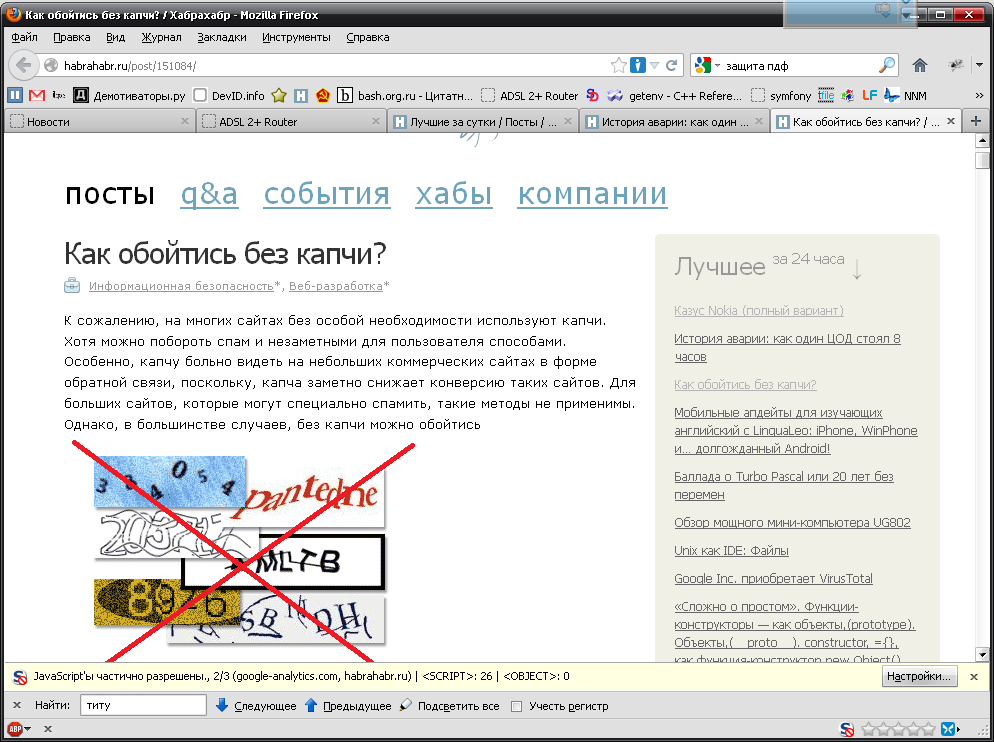
\includegraphics[scale=1,width=10cm]{ap01-09.png}
\caption{Оригінал зображення}
\label{prsc-orig:image}
\end{figure}


\begin{figure}
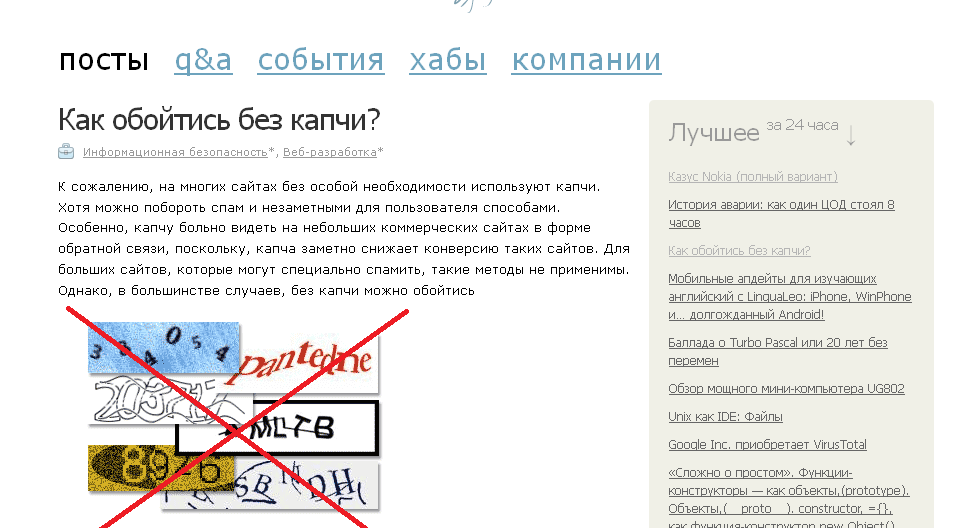
\includegraphics[scale=1,width=10cm]{ap01-10.png}
\caption{Оброблене зображення}
\label{prsc-rel:image}
\end{figure}

\begin{figure}
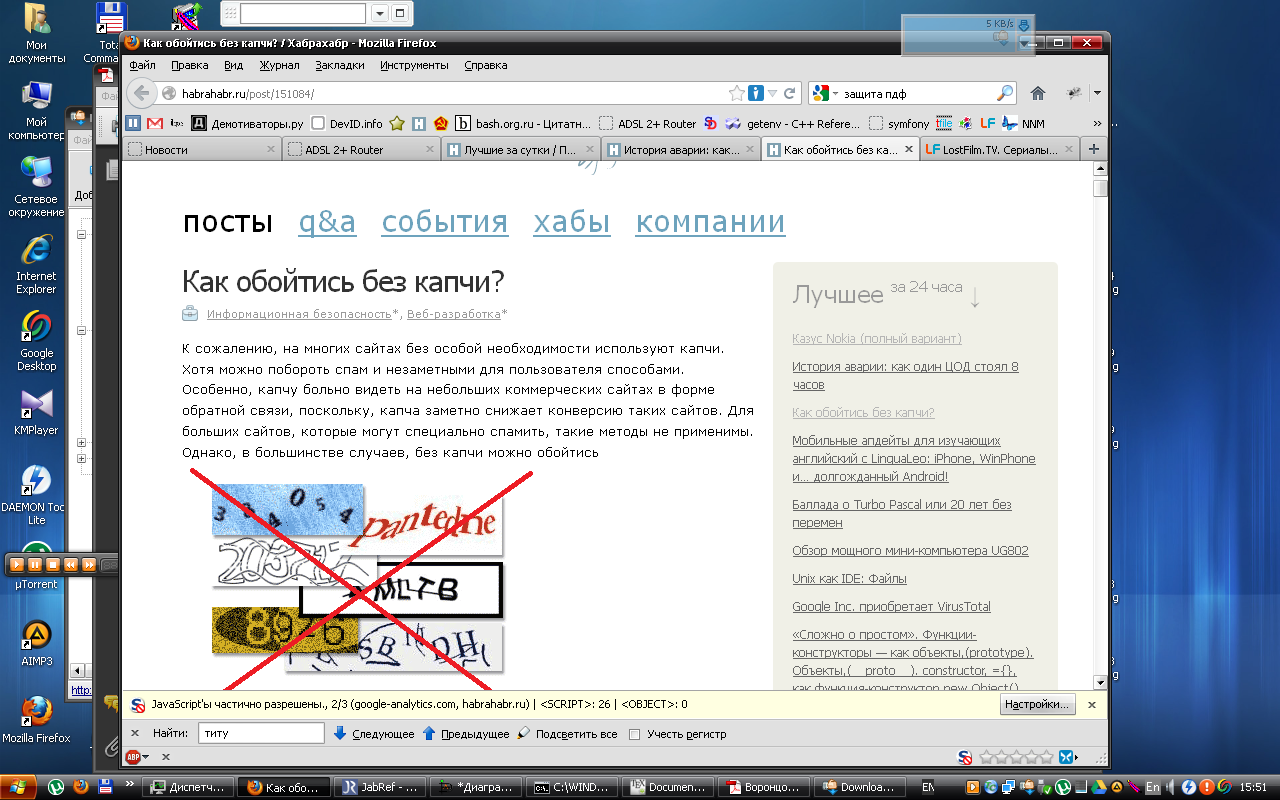
\includegraphics[scale=1,width=10cm]{ap01-11.png}
\caption{Необроблене зображення}
\label{prsc-bad:image}
\end{figure}
\chapter{Матеріали до Л/Р \No 2}
\section{Елементи форм HTML}
\index{HTML!форми}
\subsection{INPUT і його методи}
\index{HTML!форми!input}
\label{inp-tag:app}
\subsection*{Однорядкові поля введення даних}

\begin{verbatim}
<input type=text name=им'я_параметра [value=значення] 
[size=розмір_поля] [maxlen=довжина_поля]>
\end{verbatim}

Даний тег створює поле вводу з максимально допустимою довжиною тексту <<maxlen>> і розміром в size <<знакомест>>. Якщо вказаний атрибут <<value>>, то в поле буде спочатку відображатися значення даного атрибуту. У квадратних дужках \verb'[]' позначені необов'язкові атрибути.

\subsection*{Поля вводу паролів}

\begin{verbatim}
<input type=password name=им'я_параметра [value=значення] 
[size=розмір_поля] [maxlen=довжина_поля]>
\end{verbatim}

Структура даного тегу така сама як і у <input type=text>. Різниця лише у відображенні даних, що вводить користувач.


\subsection*{Приховане текстове поле}

\begin{verbatim}
<input type=hidden name=им'я_параметра [value=значення]>
\end{verbatim}

Такі поля передають дані серверу, але не відображаються на сторінці. Значення атрибуту <<value>> встановлюється при формуванні сторінки, або JavaScript-сценарієм.

\subsection*{Незалежні перемикачі}

\begin{verbatim}
<input type=checkbox name=им'я_параметра [value=значення]
[checked]>
\end{verbatim} 

Перемикач виду <<прапорець>>. У разі встановлення прапорця при відправлені форми серверу будуть передані параметри <<им'я\_параметра=значення>>. Якщо прапорець не встановлено серверу взагалі нічого не буде відправлено. 

Перемикач за замовчуванням вимкнутий, щоб зробити його увімкнутим за замовчуванням треба встановити атрибут  <<checked>>.

Стан перемикача не залежить від стану інших перемикачів цього типу.

\subsection*{Залежні перемикачі}

Залежний перемикач, так само як і незалежний перемикач, може заходитись у двох станах, в залежності від атрибуту  <<checked>>. При цьому на формі може бути увімкнений лише один перемикач серед групи перемикачів з однаковим атрибутом <<name>>.
\begin{verbatim}
<form action="http://localhost/script.php" method="GET">
<input type=radio name=answer value=yes checked>Да
<input type=radio name=answer value=no>Нет
<input type=submit value=Отправить>
</form>
\end{verbatim}

\subsection*{Кнопки відправлення та очищення параметрів форми}

Кнопка відправки служить для передачі серверу змісту форми на сторінці. Атрибут <<value>> визначає текст, ща відображається на кнопці. Під час відправлення форми серверу будуть передані дані кнопки у вигляді <<им'я\_параметра=значення>>.
\begin{verbatim}
<input type=submit [name=им'я_параметра] value=значення>
\end{verbatim}
У разі використання кнопки із зображенням сереру передадуться координати кліку відносно зображення.
\begin{verbatim}
<input type=submit [name=им'я_параметра] src=зображення>
\end{verbatim}
Кнопка очищення форми знищує всі зміни внесені користувачем сайту у дану форму.
\begin{verbatim}
<input type=reset [name=им'я_параметра] value=значення>
\end{verbatim}

\subsection*{Поле вибору файлу}

Тег <input> також дозволяє активувати діалогове вікно вибору файлу та завантажувати його на сервер при відправленні форми.
\begin{verbatim}
<input type=file name=имя [value=имя_файла]>
\end{verbatim}


\subsection{Багаторядкове текстове поле}
\index{HTML!форми!textarea}
\label{tar-tag:app}
Синтаксис багаторядкового поля виглядає наступним чином:
\begin{verbatim}
<textarea name=имя [cols=ширина_в_символах] 
[rows=высота_в_символах] wrap=тип_переноса>
текст за замовчуванням
</textarea>
\end{verbatim}
Хоча висота і ширина поля необов'язкові параметри їх бажано вказувати. Атрибут <<wrap>> відповідає за перенос і може приймати наступні значення:
\begin{enumerate}
\item Virtual --- справа від тексту з'являється полоса прокрутки, а текст розбивається на рядки.
\item Physical --- залежить від браузера і виглядає по-різному
\item None --- текст залишається у тому вигляді, в якому користувач його ввів, з'являються горизонтальна і вертикальна полоси прокрутки.
\end{enumerate}

\subsection{Списки з вибором} \label{sel-tag:app}
\index{HTML!форми!select}
\subsection*{Списки з одиночним вибором}
\label{sel-tag:app}
Списки з одиночним вибором реалізуються за допомогою наступної конструкції:
\begin{verbatim}

<select name=day size=1>
<option value=1>Понедельник</option>
<option value=2>Вторник</option>
<option value=3 selected>Среда</option>
<option value=4>Четверг</option>
<option value=5>Пятница</option>
<option value=6>Суббота</option>
<option value=7>Воскресенье</option>
</select>

\end{verbatim}
При відправленні форми сервер отримає дані виду <<им'я\_параметра=значення>>. За замовчуванням може бути обраний пункт списку серед атрибутів якого є \verb'selected'.

\subsection*{Списки з множинним вибором}
Список з множинним вибором відрізняється лише атрибутом \verb'multiple' в середині тега \verb'<select>'.
\begin{verbatim}

<select name=day size=7 multiple>
<option value=1>Понедельник</option>
<option value=1>Вторник</option>
<option value=1>Среда</option>
<option value=1>Четверг</option>
<option value=1>Пятница</option>
<option value=1>Суббота</option>
<option value=1>Воскресенье</option>
</select>


\end{verbatim}


\section{Змінні-функції}
\index{PHP!функції!змінні-функції}
\label{var-func:app}
Приклад використання змінної-функції:
\begin{verbatim}
<?php
?php
function foo() {
    echo "In foo()<br />\n";
}
function bar($arg = '')
{
    echo "In bar(); argument was '$arg'.<br />\n";
}
// Функция-обертка для echo
function echoit($string)
{
    echo $string;
}

$func = 'foo';
$func();        // Вызывает функцию foo()
$func = 'bar';
$func('test');  // Вызывает функцию bar()
$func = 'echoit';
$func('test');  // Вызывает функцию echoit()
\end{verbatim}
\chapter{Матеріали до Л/Р \No 3}

\section{Змінні оточення web-сервера Apache}
\label{var-apa:app}
\nopagebreak[4]
\index{Web-сервери!Apache!змінні оточення}
\subsection{Формовані сервером змінні}

\textbf{AUTH\_TYPE} Використовується схема аутентифікації. Зазвичай BASIC

\textbf{CONTENT\_LENGTH} Довжина вмісту

\textbf{CONTENT\_TYPE} MIME-тип вмісту

\textbf{GETAWAY\_INTERFACE} Версія CGI, наприклад CGI/1.1

\textbf{PATH\_info} HTTP-шлях до сценарію

\textbf{PATH\_TRANSLATED} Повний шлях до сценарію

\textbf{REMOTE\_ADDR} IP-адреса запитуваного комп'ютера-клієнта

\textbf{REMOTE\_HOST} Доменне ім'я запитувача комп'ютера (якщо доступно). Доменне ім'я визначається веб-сервером за допомогою служби DNS. Директива \verb'HostnameLookups' сервера Apache дозволяє (або забороняє) перетворення IP-адреси в доменне ім'я.

\textbf{REMOTE\_PORT} Порт, закріплений за браузером для отримання відповіді від сервера

\textbf{REMOTE\_USER} Ім'я користувача, що пройшов аутентифікацію

\textbf{QUERY\_STRING} Рядок переданих серверу параметрів

\textbf{SERVER\_ADDR} IP-адресу сервера

\textbf{SERVER\_NAME} Доменне ім'я сервера. Визначається директивою ServerName файлу конфігурації

\textbf{SERVER\_PORT} TCP-порт Web-сервера. Зазвичай 80

\textbf{SERVER\_PROTOCOL} Версія протоколу HTTP. Наприклад, HTTP/1.1

\textbf{SERVER\_SOFTWARE} Програмне забезпечення сервера

\textbf{SCRIPT\_NAME} HTTP-шлях до сценарію

\textbf{SCRIPT\_FILENAME} Файл сценарію в файловій системі сервера (фізичний шлях). Наприклад, \verb'/var/www/cgi-bin/script.cgi'


\subsection{Спеціальні змінні сервера Apache}

\textbf{DOCUMENT\_ROOT} Фізичний шлях до кореневого WWW-каталогу сервера. Наприклад, \verb'/var/www.html/'

\textbf{SERVER\_ADMIN} Адреса електронної пошти адміністратора сервера

\textbf{SERVER\_SIGNATURE} Підпис сервера. Наприклад, <<\verb'Apache/1.3.3 сервера на www.somefirm.com порт 80'>>


\subsection{Змінні HTTP-полів запиту}

\textbf{HTTP\_HOST} Ім'я віртуального хоста, якому адресовано запит

\textbf{HTTP\_USER\_AGENT} Програмне забезпечення віддаленого користувача. Зазвичай ця змінна оточення містить назву і версію браузера

\textbf{HTTP\_ACCEPT} Список підтримуваних клієнтом типів інформації. 

\textbf{HTTP\_ACCEPT\_LANGUAGE} Список підтримуваних мов в порядку переваги, наприклад, RU, EN

\textbf{HTTP\_ACCEPT\_ENCODING} Список підтримуваних методів стиснення

\textbf{HTTP\_ACCEPT\_CHARSET} Список підтримуваних кодувань

\textbf{HTTP\_CONNECTION} Тип з'єднання. Можливі два варіанти:
\begin{list}{•}{•}
\item \verb'Keep-Alive'~--- якщо після відповіді на запит не потрібно розривати з'єднання;
\item \verb'Close'~--- якщо потрібно закрити з'єднання відразу після відповіді на запит.
\end{list}

\textbf{HTTP\_REFERER} Значення поля \verb'REFERER'. У цьому полі браузер передає URL ресурсу, який посилається на наш сервер. Наприклад, якщо користувач перейшов на сайт зі сторінки http://www.somehost.com/page.php, то значення поля \verb'REFERER' буде http://www.somehost.com/page.php.

\textbf{HTTP\_X\_FORWARDED\_FOR} Якщо користувач працює через проксі-сервер, то в цьому полі буде IP-адреса комп'ютера, який звернувся до проксі-сервера. Якщо це поле вже містить значення, то нове значення буде додано через кому.



\subsection{Суперглобальні масиви PHP}
\index{PHP!змінні!суперглобальні масиви}
\label{sup-glob:app}

\textbf{\$GLOBALS}~--- масив всіх глобальних змінних (у тому числі і для користувача).

\textbf{\$\_SERVER}~--- містить безліч інформації про поточний запит і сервер.

\textbf{\$\_ENV}~--- поточні змінні середовища. Їх набір специфічний для кожної конкретної платформи, на якій виконується сценарій.

\textbf{\$\_GET}~--- асоціативний масив з параметрами GET-запиту. У початковому вигляді ці параметри доступні в \verb|$_SERVER ['QUERY\_STRING']| і в \verb|$_SERVER ['REQUEST_URI']| в складі URI.

\textbf{\$\_POST}~--- асоціативний масив значень полів HTML-форми при відправки методом POST.

\textbf{\$\_FILES}~--- асоціативний масив з відомостями про надіслані методом POST файлах. Кожен елемент має індекс ідентичний значенню атрибута \verb'name' у формі і, в свою чергу, також є масивом з наступними елементами:
\begin{enumerate}
\item \verb|$_FILES['name']|~--- вихідне ім'я файлу на комп'ютері користувача.
\item \verb|$_FILES['type']|~--- зазначений агентом користувача MIME~--- тип файлу.
\item \verb|$_FILES['size']|~--- розмір файлу в байтах.
\item \verb|$_FILES['tmp_name']|~--- повний шлях до файлу в тимчасовій папці.
\item \verb|$_FILES['error']|~--- код помилки.
\end{enumerate}

\textbf{\$\_COOKIE}~--- асоціативний масив з переданими агентом користувача значеннями cookie.

\textbf{\$\_REQUEST}~--- загальний масив ввідних даних запиту користувача як в масивах \verb'$_GET, $_POST, $_COOKIE'. Починаючи з версії PHP 4.1 включається і вміст \verb'$_FILES'.


\section{Пріоритети виконання операторів}
\index{PHP!оператори!пріоритети}


\begin{center}
\begin{longtable}[t]{|c|p{25em}|}
\caption{Пріоритети виконання операторів} \label{pr-op:table}\\
\hline

Асоціативність & Оператор \\
\hline \endfirsthead
\caption*{\space Продовження} \\
\hline
Асоціативність & Оператор \\
\hline \endhead
\hline \endfoot
неасоціативна	& \verb|new| \\
права	& \verb|[|\\
неасоціативна	& \verb|++ --| \\
неасоціативна	& \verb|! ~ -(int) (float) (string) (array) (object) @| \\
ліва	& \verb|* / %| \\
ліва	& \verb|+ - .| \\
ліва	& \verb|<< >>| \\
неассоціативна	& \verb|< <= > >=| \\
неассоціативна	& \verb|== != === !==| \\
ліва	& \verb|&| \\
ліва	& \verb|^| \\
ліва	& \verb'|' \\
ліва	& \verb|&&| \\
ліва	& \verb'||' \\
ліва	& \verb|? :| \\
права	& \verb'= += -= *= /= .= %= &= |= ^= <<= >>='  \\
\penalty -10000
ліва	& \verb|and| \\
ліва	& \verb|xor| \\
ліва	& \verb|or| \\
ліва	& \verb|,| \\

\hline
\end{longtable}
\end{center}
\chapter{Матеріали до Л/Р \No 4}

\section{Рядки та регулярні вирази}
\subsection{Функції роботи з рядками}
\label{str-func:app}
\nopagebreak[4]


\index{PHP!змінні!рядки!функції}
\begin{longtable}[t]{|l|p{21em}|}

\caption{\space Повний список функцій роботи з рядками} \label{str-func:table}\\
\hline

Функція & Опис \\
\hline \endfirsthead
\caption*{\space Продовження} \\
\hline
Функція & Опис \\
\hline \endhead
\hline \endfoot
addcslashes & екрануючі спецсимволи в стилі мови C \\
addslashes & екрануючі спецсимволи в рядку \\
bin2hex & Перетворює бінарні дані у шістнадцятірічне подання \\
chr & Повертає символ за його кодом \\
chunk\_split & Розбиває рядок на фрагменти \\
convert\_cyr\_string & Перетворює рядок з одного кириличної кодування в інше \\
count\_chars & Повертає інформацію про символи, що входять в рядок \\
crc32 & Обчислює CRC32 для рядка \\
crypt & Необоротне шифрування (хешування) \\
echo & Виводить одну чи більше рядків \\
explode & Розбиває рядок на підрядки \\
fprintf & Записує отформатированную рядок у потік \\
get\_html\_translation\_table & Повертає таблицю перетворень \\
hebrev & Перетворює текст на івриті з логічного кодування у візуальне \\
hebrevc & Перетворює текст на івриті з логічнго кодування у візуальне з перетворенням в переклад \\
htmlentities & Перетворює символи у відповідні HTML теги \\
htmlspecialchars & Перетворює спеціальні символи в HTML теги \\
html\_entity\_decode & Перетворює HTML теги в відповідні символи \\
implode & Об'єднує елементи масиву в рядок \\
localeconv & Повертає інформацію про числові формати \\
ltrim & Видаляє пробіли з початку рядка \\
md5 & Повертає MD5-хеш рядка \\
md5\_file & Повертає MD5-хеш файлу \\
metaphone & Повертає ключ metaphone для рядка \\
nl2br & Вставляє HTML-код розриву рядка перед кожним переведенням рядка \\
number\_format & Форматує число з поділом груп \\
ord & Повертає ASCII-код символу \\
parse\_str & Розбирає рядок у змінні \\
print & Виводить рядок \\
printf & Виводить відформатований рядок \\
quoted\_printable\_decode & розкодує рядок, закодовану методом quoted printable \\
quotemeta & екрануючі спеціальні символи \\
rtrim & Видаляє пробіли з кінця рядка \\
sha1 & Повертає SHA1-хеш рядка \\
sha1\_file & Повертає SHA1-хеш файлу \\
similar\_text & Обчислює ступінь схожості двох рядків \\
soundex & Повертає ключ soundex для рядка \\
sprintf & Повертає відформатований рядок \\
sscanf & Розбирає рядок у відповідності із заданим форматом \\
strcasecmp & Порівняння рядків без урахування регістра, безпечне для даних у двійковій формі \\
strcmp & Порівняння рядків, безпечне для даних у двійковій формі \\
strcoll & Порівняння рядків з урахуванням поточної локалі \\
strcspn & Повертає довжину ділянки на початку рядка, не відповідного  масці \\
stripcslashes & Видаляє екранування символів, вироблене функцією addcslashes () \\
stripos & Повертає позицію першого входження підрядка без урахування регістра \\
stripslashes & Видаляє екранування символів, вироблене функцією addslashes () \\
strip\_tags & Видаляє HTML і PHP теги з рядка \\
stristr & Аналог функції strstr, але незалежний від регістру \\
strlen & Повертає довжину рядка \\
strnatcasecmp & Порівняння рядків без урахування регістра з використанням алгоритму \\
strnatcmp & Порівняння рядків з використанням алгоритму "природнього упорядкування" \\
strncasecmp & порівняння перших n символів рядків без урахування регістра, безпечне для даних у двійковій формі \\
strncmp & порівняння перших n символів рядків без урахування регістра, безпечне для даних у двійковій формі \\
strpos & Знаходить перше входження підрядка в рядок \\
strrchr & Знаходить останнє входження символу в рядок \\
strrev & Перевертає рядок \\
strripos & Повертає позицію останнього входження підрядка без урахування регістра \\
strrpos & Знаходить останнє входження символу в рядок \\
strspn & Повертає довжину ділянки на початку рядка, відповідного масці \\
strstr & Знаходить перше входження підрядка \\
strtok & Розбиває рядок \\
strtolower & Перетворює рядок у нижній регістр \\
strtoupper & Перетворює рядок у верхній регістр \\
strtr & Перетворює задані символи \\
str\_ireplace & Регістро-незалежний варіант функції str\_replace (). \\
str\_pad & Доповнює рядок інший рядком до заданої довжини \\
str\_repeat & Повертає повторювану рядок \\
str\_replace & Замінює рядок пошуку на рядок заміни \\
str\_rot13 & Виконує над рядком перетворення ROT13 \\
str\_shuffle & перемішує символи в рядку \\
str\_split & Розбиває рядок в масив \\
str\_word\_count & Повертає інформацію про слова, що входять в рядок \\
substr & Функція повертає частину рядка \\
substr\_count & Підраховує кількість входжень підрядка в рядок \\
substr\_replace & Замінює частину рядка \\
trim & Видаляє пробіли з початку та кінця рядка \\
ucfirst & Перетворює перший символ рядка в верхній регістр \\
ucwords & Перетворює у верхній регістр перший символ кожного слова в рядку \\
vprintf & Виводить відформатований рядок \\
vsprintf & Повертає відформатований рядок \\
wordwrap & Виконує перенесення рядка на дану кількість символів з використанням символу розриву рядка \\
\hline
\end{longtable}

\subsection{Метасимволи та керуючі конструкцію регулярних виразів у MySQL}
\label{chr-rxp:app}
\index{PHP!регулярні вирази}
У додатку надано перелік метасимволів та керуючих конструкцій для регулярних виразів, що підтримуються у СУБД MySQL.  

\pagebreak[4]
\begin{longtable}[t]{|l|p{20em}|}
\caption{Спецпослідовності регулярних виразів POSIX 1003.2 для MySQL} \label{chr2-rxp:table}\\
\hline

Позначення & Опис \\
\hline

\verb'\t' & символ табуляции. \\
\verb'\f' & конец файла. \\
\verb'\n' & символ перевода строки. \\
\verb'\r' & символ возврата каретки. \\
\verb'\\' & символ обратного слэша \verb'\'. \\


\hline
\end{longtable}


\pagebreak[3]

\begin{longtable}[t]{|l|p{20em}|}

\caption{Опис метасимволів регулярних виразів POSIX 1003.2 для MySQL} \label{chr-rxp:table}\\
\hline

Позначення & Опис \\
\hline




\verb|^| & Відповідає початку рядка. \\

\verb|$| & Відповідає кінцю рядка. \\

\verb|.| & Відповідає будь-якому символу. \\

\verb|a*| & Відповідає будь-якій послідовності з 0 або більше символів <<a>>. \\

\verb|a+| & Відповідає будь-якій послідовності з 1 або більше символів <<a>>. \\

\verb|a?| & Відповідає 0 або 1 символу <<a>>. \\

\verb'de|abc' & Відповідає послідовності <<de>> або <<abc>>. \\

\verb|(abc)*| & Відповідає 0 або більше послідовностям <<abc>>.  \\

\verb|[a-dX],[^a-dX]| & Відповідає будь-якому символу, який є (або не яв ляется, якщо використовується \verb|^|) будь-яким із символів а, Ь, с, d або X. Символ '-' між двома іншими символами утворює інтервал. \\
  
\hline
\end{longtable}


\pagebreak[3]



\begin{longtable}[t]{|l|p{20em}|}

\caption{Класи символів регулярних виразів POSIX 1003.2 для MySQL} \label{chr3-rxp:table}\\
\hline

Позначення & Опис \\
\hline


\verb|[:alnum:]| & алфавітно цифрові символи. \\
\verb|[:alpha:]| & символи алфавіту. \\
\verb|[:blank:]| & символи пробілу і табуляції. \\
\verb|[:cntrl:]| & керуючі символи. \\
\verb|[:digit:]| & десяткові цифри (0-9). \\
\verb|[:graph:]| & графічні (видимі) символи. \\
\verb|[:lower:]| & символи алфавіту в нижньому регістрі. \\
\verb|[:print:]| & графічні або невидимі символи. \\
\verb|[:punct:]| & знаки пунктуації. \\
\verb|[:space:]| & символи пробілу, табуляції, нового рядка або повернення каретки. \\
\verb|[:upper:]| & символи алфавіту в верхньому регістрі. \\
\verb|[:xdigit:]| & шістнадцяткові цифри. \\

\hline
\end{longtable}


\pagebreak[3]




\chapter{Матеріали до Л/Р \No 5}



\section{Функції для роботи з файловою системою}
\index{Файл!функції}
\begin{longtable}[t]{|l|p{20em}|}
\kill
\caption{\space Перелік функцій для роботи з ФС} \label{fs-funcr:table}\\
\hline

функція & Опис \\
\hline \endfirsthead
\caption*{\space Продовження} \\
\hline
функція & Опис \\
\hline \endhead
\hline \endfoot



\verb'basename' & Повертає останній компонент імені з вказаного шляху\\
\verb'chgrp' & Змінює групу власників файлу\\
\verb'chmod' & Змінює режим доступу до файлу\\
\verb'chown' & Змінює власника файлу\\
\verb'clearstatcache' & Очищає кеш стану файлів\\
\verb'copy' & Копіює файл\\
\verb'delete' & См.опис функції unlink або unset\\
\verb'dirname' & Повертає ім'я батьківського каталогу з зазначеного шляху\\
\verb'disk_free_space' & Повертає розмір доступного простору в каталозі або в файловій системі\\
\verb'disk_total_space' & Повертає загальний розмір каталогу або розділу файлової системи\\
\verb'diskfreespace' & Псевдонім disk\_free\_space\\
\verb'fclose' & Закриває відкритий дескриптор файлу\\
\verb'feof' & Перевіряє, чи досягнутий кінець файлу\\
\verb'fflush' & Скидає буфер виводу у файл\\
\verb'fgetc' & Зчитує символ з файлу\\
\verb'fgetcsv' & Читає рядок з файлу і виробляє розбір даних CSV\\
\verb'fgets' & Читає рядок з файлу\\
\verb'fgetss' & Читає рядок з файлу і відкидає HTML-теги\\
\verb'file_exists' & Перевіряє наявність вказаного файлу або каталогу\\
\verb'file_get_contents' & Читає вміст файлу в рядок\\
\verb'file_put_contents' & Пише рядок в файл\\
\verb'file' & Читає вміст файлу і поміщає його в масив\\
\verb'fileatime' & Повертає час останнього доступу до файлу\\
\verb'filectime' & Повертає час зміни індексного дескриптора файлу\\
\verb'filegroup' & Отримує ідентифікатор групи файлу\\
\verb'fileinode' & Повертає індексний дескриптор файлу\\
\verb'filemtime' & Повертає час останньої зміни файлу\\
\verb'fileowner' & Повертає ідентифікатор власника файлу\\
\verb'fileperms' & Повертає інформацію про права на файл\\
\verb'filesize' & Повертає розмір файлу\\
\verb'filetype' & Повертає тип файлу\\
\verb'flock' & Переносима консультативна блокування файлів\\
\verb'fnmatch' & Перевіряє збіг імені файлу з шаблоном\\
\verb'fopen' & Відкриває файл або URL\\
\verb'fpassthru' & Виводить всі залишилися дані з файлового покажчика\\
\verb'fputcsv' & Форматує рядок у вигляді CSV і записує його в файловий покажчик\\
\verb'fputs' & Псевдонім fwrite\\
\verb'fread' & бінарних-безпечне читання файлу\\
\verb'fscanf' & Обробляє дані з файлу відповідно до формату\\
\verb'fseek' & Встановлює зсув у файловому покажчику\\
\verb'fstat' & Отримує інформацію про фото використовуючи відкритий файловий покажчик\\
\verb'ftell' & Повідомляє поточну позицію читання/запису файлу\\
\verb'ftruncate' & Врізає файл до вказаної довжини\\
\verb'fwrite' & бінарно-безпечний запис в файл\\
\verb'glob' & Знаходить файлові шляху, що збігаються з шаблоном\\
\verb'is_dir' & Визначає, чи є ім'я файлу директорією\\
\verb'is_executable' & Визначає, чи є файл виконуваним\\
\verb'is_file' & Визначає, чи є файл звичайним файлом\\
\verb'is_link' & Визначає, чи є файл символічним посиланням\\
\verb'is_readable' & Визначає наявність файлу і доступний він для читання\\
\verb'is_uploaded_file' & Визначає, чи був файл завантажений за допомогою HTTP POST\\
\verb'is_writable' & Визначає, чи доступний файл для запису\\
\verb'is_writeable' & Псевдонім is\_writable\\
\verb'lchgrp' & Змінює групу, якій належить символічне посилання\\
\verb'lchown' & Змінює власника символічного посилання\\
\verb'link' & Створює жорстке посилання\\
\verb'linkinfo' & Повертає інформацію про посиланню\\
\verb'lstat' & Повертає інформацію про фото або символічної посиланню\\
\verb'mkdir' & Створює директорію\\
\verb'move_uploaded_file' & Переміщає завантажений файл у нове місце\\
\verb'parse_ini_file' & Обробляє конфігураційний файл\\
\verb'parse_ini_string' & Розбирає рядок конфігурації\\
\verb'pathinfo' & Повертає інформацію про шлях до файлу\\
\verb'pclose' & Закриває файловий покажчик процесу\\
\verb'popen' & Відкриває файловий покажчик процесу\\
\verb'readfile' & Виводить файл\\
\verb'readlink' & Повертає файл, на який вказує символьне посилання\\
\verb'realpath_cache_get' & Отримує записи з кешу реального шляху\\
\verb'realpath_cache_size' & Отримує розмір кеша реального шляху\\
\verb'realpath' & Повертає канонізований абсолютний шлях до файлу\\
\verb'rename' & Перейменовує файл або директорію\\
\verb'rewind' & Скидає курсор у файлового покажчика\\
\verb'rmdir' & Видаляє директорію\\
\verb'set_file_buffer' & Псевдонім stream\_set\_write\_buffer\\
\verb'stat' & Повертає інформацію про файл\\
\verb'symlink' & Створює символічну посилання\\
\verb'tempnam' & Створює файл з унікальним ім'ям\\
\verb'tmpfile' & Створює тимчасовий файл\\
\verb'touch' & Встановлює час доступу і модифікації файлу\\
\verb'umask' & Змінює поточну umask\\
\verb'unlink' & Видаляє файл \\


\hline
\end{longtable}



\section{Параметри функції <<fopen()>>}
\begin{longtable}[t]{|c|p{27em}|}
\kill
\caption{\space Другий параметр функції <<fopen()>>} \label{fo-par:table}\\
\hline

Параметр & Опис \\
\hline \endfirsthead
\caption*{\space Продовження} \\
\hline
Параметр & Опис \\
\hline \endhead
\hline \endfoot
\verb'R' & Відкриває файл тільки для читання; поміщає покажчик в початок файлу. \\ \hline
\verb'R+' & Відкриває файл для читання і запису; поміщає покажчик в початок файлу. \\ \hline
\verb'W' & Відкриває файл тільки для запису; поміщає покажчик в початок файлу і обрізає файл до нульової довжини. Якщо файл не існує~--- намагається його створити. \\ \hline
\verb'W+' & Відкриває файл для читання і запису; поміщає покажчик в початок файлу і обрізає файл до нульової довжини. Якщо файл не існує~--- намагається його створити. \\ \hline
\verb'A' & Відкриває файл тільки для запису; поміщає покажчик в кінець файлу. Якщо файл не існує~--- намагається його створити. \\ \hline
\verb'A+' & Відкриває файл для читання і запису; поміщає покажчик в кінець файлу. Якщо файл не існує~--- намагається його створити. \\ \hline
\verb'X' & Створює і відкриває тільки для запису; поміщає покажчик в початок файлу. Якщо файл вже існує, виклик \verb'fopen()' закінчиться невдачею, поверне \verb'FALSE' і видасть помилку \verb'E_WARNING'. Якщо файл не існує, спробує його створити. \\ \hline
\verb'X+' & Створює і відкриває для читання і запису інакше поверне \verb'FALSE'. \\ \hline
\verb'C' & Відкриває файл тільки для запису. Якщо файл не існує, то він створюється. Якщо ж файл існує, то він не обрізається, і виклик цієї функції не викликає помилку. Покажчик на файл буде встановлений на початок файлу.\\ \hline
\verb'C+' & Відкриває файл для читання і запису інакше функція має ту ж поведінку, що і з використанням <<\verb'c'>>. \\ \hline

\hline
\end{longtable}


\section{Функції для роботи з каталогами}
\index{Каталог!функції}
\begin{longtable}[t]{|c|p{27em}|}
\kill
\caption{\space Перелік функцій для роботи з каталогами} \label{dir-func:table}\\
\hline

Функція & Опис \\
\hline \endfirsthead
\caption*{\space Продовження} \\
\hline
Функція & Опис \\
\hline \endhead
\hline \endfoot
\verb'chdir' & Змінює каталог\\
\verb'mkdir' & Створює каталог\\
\verb'rmdir' & Видаляє каталог\\
\verb'is_dir' & Перевіряє чи є об'єкт каталогом\\
\verb'chroot' & Змінює кореневий каталог\\
\verb'closedir' & Звільняє дескриптор каталогу\\
\verb'dir' & Повертає екземпляр класу Directory\\
\verb'getcwd' & Отримує ім'я поточного робочого каталога\\
\verb'opendir' & Відкриває дескриптор каталогу\\
\verb'readdir' & Отримує елемент каталогу за його дескриптору\\
\verb'rewinddir' & Скинути дескриптор каталогу\\
\verb'scandir' & Отримує список файлів і каталогів, розташованих по зазначеному шляху \\

\hline
\end{longtable}

\chapter{Матеріали до Л/Р \No 6}


\section{Налаштування сесії у РНР}
\index{Сесії!налаштування}
\begin{longtable}[t]{|l|p{20em}|}
\kill
\caption{\space Перелік параметрів у файлі php.ini} \label{ses-opt:table}\\
\hline

Опція & Опис \\
\hline \endfirsthead
\caption*{\space Продовження} \\
\hline
Опція & Опис \\
\hline \endhead
\hline \endfoot

\verb'session.save_path' & визначає, де на сервері зберігатимуться дані сесії. \\
\verb'session.use_cookies' & визначає, чи використовувати cookies при роботі з сесіями.\\
\verb'session.cookie_lifetime' & задає тривалість життя cookies в секундах.\\
\verb'session.name' & визначає ім'я сесії\\
\verb'session.auto_start' & дозволяє автоматично запускати сесії\\
\verb'session.serialize_handler' & задає спосіб кодування даних сесії\\
\verb'session.cache_expire' & визначає, через скільки хвилин застаріває документ в кеші\\

\hline
\end{longtable}

Ім'я сесії \verb'session.name' за умовчанням встановлюється як \verb'PHPSESSID' і використовується в \verb'cookies' як ім'я змінної, в якій зберігається ідентифікатор сесії. Автоматичний запуск сесій за замовчуванням відключений, але його можна задати, зробивши значення \verb'session.auto_start' рівним <<1>>. Для кодування даних сесії по замовчуванню використовується php. Старіння даних, збережених в кеші, відбувається через 180 хвилин.

\section{Повний перелік змінних у <<php.ini>>}
\begin{longtable}[t]{|l|p{15em}|}
\kill

\caption{\space Повний параметрів у файлі <<php.ini>> та значень за замовчуванням} \label{ses-opt-full:table}\\
\hline

Опція & Значення \\
\hline \endfirsthead
\caption*{\space Продовження} \\
\hline
Опція & Значення \\
\hline \endhead
\hline \endfoot

\verb'session.save_path' & \verb'""'\\
\verb'session.name' & "PHPSESSID"\\
\verb'session.save_handler' & "files"\\
\verb'session.auto_start' & "0"\\
\verb'session.gc_probability' & "1"\\
\verb'session.gc_divisor' & "100"\\
\verb'session.gc_maxlifetime' & "1440"\\
\verb'session.serialize_handler' & "php"\\
\verb'session.cookie_lifetime' & "0"\\
\verb'session.cookie_path' & "/"\\
\verb'session.cookie_domain' & \verb'""'\\
\verb'session.cookie_secure' & \verb'""'\\
\verb'session.cookie_httponly' & \verb'""'\\
\verb'session.use_cookies' & "1"\\
\verb'session.use_only_cookies' & "1"\\
\verb'session.referer_check' & \verb'""'\\
\verb'session.entropy_file' & \verb'""'\\
\verb'session.entropy_length' & "0"\\
\verb'session.cache_limiter' & "nocache"\\
\verb'session.cache_expire' & "180"\\
\verb'session.use_trans_sid' & "0"\\
\verb'session.bug_compat_42' & "1"\\
\verb'session.bug_compat_warn' & "1"\\
\verb'session.hash_function' & "0"\\
\verb'session.hash_bits_per_character' & "4"\\
\verb'url_rewriter.tags' & "a=href, area=href, frame=src, form=, fieldset="\\
\verb'session.upload_progress.enabled' & "1"\\
\verb'session.upload_progress.cleanup' & "1"\\
\verb'session.upload_progress.prefix' & "upload\_progress\_"\\
\verb'session.upload_progress.name' & "PHP\_SESSION\_ UPLOAD\_PROGRESS"\\
\verb'session.upload_progress.freq' & "1\%"\\
\verb'session.upload_progress.min_freq' & "1"\\


\hline
\end{longtable}


\section{Опис функцій для роботи з сесіями}
\index{PHP!функції!сесії}
\label{ses-func:text}
Нижче дано перелік функцій, що необхідні для роботи із сесіями. Деякі функції налаштування дублюють функціонал опцій у файлі <<php.ini>>, на такі функції буде звернено увагу.

\textbf{session\_destroy()}

Функція скасовує дію \verb'session_start()'. Викликати потрібно після виклику \verb'session_start()'. Можна застосовувати, щоб знищувати сессіію користувача, а потім відразу викликати в програмі вдруге \verb'session_start()', вийти зовсім новий відвідувач з новим ідентифікатором і чистої сесією.

\textbf{session\_name()} або \verb'session.name'

РНР для зберігання ідентифікатора використовує якусь змінну. В cookies записують змінну: значення змінної~--- ідентифікатор, назва змінної~--- PHPSESSID. PHPSESSID~--- це назва, яку використовують за замовчуванням. Її можна перейменувати у щось більш коротке, наприклад SID. А для цього треба замінити параметр \verb'session.name' на значення SID: 

можна замінити php.ini: \verb'session.name = SID' 

можна створити. htaccess файл у каталозі з скриптами вашого сайту і помістити рядок \verb'php_value session.name SID'

Щоб отримати назву змінної, яку використовують для зберігання ідентифікатора, треба скористатися функцією без параметра \$name = \verb'session_name()'.

Щоб встановити таку змінну в довільну назву, скористайтеся функцією з параметром \verb'session_name("МояНазва")'. Зрозуміло, якщо Вам чомусь знадобилося змінити ім'я змінної для cookies за допомогою цієї функції, то її треба викликати перед \verb'session_start()' або \verb'session_register()'.

\textbf{session\_module\_name()} або \verb'session_save_handler'

Отримати або встановити поточний модуль сесії. РНР може зберігати сесії різному вигляді. За замовчуванням~--- в файлах.

\textbf{session\_save\_path()} або \verb'session.save_path'

Отримати або встановити каталог, в якому будуть зберігатися файли сесії. \$path = \verb'session_save_path()'~--- отримати. \verb'session_save_path("/mydir/temp")'~--- встановити. Параметр \verb'session.save_path' можна задавати в php.ini або <<.htaccess>>. 

\textbf{session\_id()}

Отримати або встановити ідентифікатор відвідувача (128-бітове число, представлене у вигляді рядка в 32 байти). У нормальних умовах Вам не потрібно встановлювати номер сесії. Але якщо Ви хочете для всіх своїх відвідувачів використовувати одну сессіію, то перед \verb'session_start()' придумайте будь-яке ім'я (наприклад, \verb'session_id ("my_name")') або отримаєте справжній ідентифікатор іншим чином. Виклик функції без параметрів поверне Вам поточний номер сесії (в такому випадку~--- викликати після \verb'session_start()').

\textbf{session\_register()}

Зареєструвати одну або кілька змінних. Передавати треба імена змінних, а не їх значення: \verb'session_register("змінна1", "змінна2", ...)'. 

\textbf{session\_unregister()}

Видалити з сесії необхідну змінну. Можна передати тільки одне ім'я змінної за один виклик функції.

\textbf{session\_unset()}

Очистити всі змінні сесії. У відмінності від \verb'session_destroy()' сесія і ідентифікатор залишається.

\textbf{session\_is\_registered()}

Перевірити, зареєстрована якась змінна в поточній сесії чи ні:

\verb'if (session_is_registered("змінна")) ...'

\textbf{session\_get\_cookies\_params()} і

\textbf{session\_set\_cookies\_params()}

Отримати інформацію про cookies, що зберігає змінну з ідентифікатором сесії, можна наступним чином:

\begin{verbatim}
echo "<pre> session INFO: \ n";
print_r (session_get_cookies_params());
\end{verbatim}

Так можна дізнатися про час життя змінної, домен та шляхи cookies.

Функцією \verb'session_set_cookies_params()' можна перевстановити параметри (хоча всі ці параметри задані в php.ini).

\textbf{session\_decode()} і \textbf{session\_encode()}

Декодування закодованих рядків у сесії і кодування змінних у рядок сесії.

\textbf{session\_set\_save\_handler()}

Можливо, Вас не влаштовують варіанти зберігання сесій, що пропонуються в РНР. Може бути, ви хочете зберігати сесії в простих текстових файлах, щоб їх можна було легко редагувати. Тоді Вам потрібно створити декілька функцій, що відповідають за функціонування сесій і передати назви цих функцій в \verb'session_set_save_handler()'.

\chapter{Матеріали до Л/Р \No 7}
\section{Синтаксис команди CREATE TABLE}
\index{MySQL!SQL!CREATE}
\label{crtab:text}
\begin{verbatim}
 CREATE [TEMPORARY] TABLE [IF NOT EXISTS] 
 tbl_name [(create_definition, ...)]
 [Table_options] [select_statement]

 create_definition:
   col_name type [NOT NULL | NULL] [DEFAULT default_value] 
   [AUTO_INCREMENT] [PRIMARY KEY] [reference_definition]
   або PRIMARY KEY (index_col_name, ...)
   або KEY [index_name] (index_col_name, ...)
   або INDEX [index_name] (index_col_name, ...)
   або UNIQUE [INDEX] [index_name] (index_col_name, ...)
   або FULLTEXT [INDEX] [index_name] (index_col_name, ...)
   або [CONSTRAINT symbol] FOREIGN KEY [index_name] 
       (index_col_name, ...) [Reference_definition]
   або CHECK (expr)

 type:
         TINYINT [(length)] [UNSIGNED] [ZEROFILL]
   або SMALLINT [(length)] [UNSIGNED] [ZEROFILL]
   або MEDIUMINT [(length)] [UNSIGNED] [ZEROFILL]
   або INT [(length)] [UNSIGNED] [ZEROFILL]
   або INTEGER [(length)] [UNSIGNED] [ZEROFILL]
   або BIGINT [(length)] [UNSIGNED] [ZEROFILL]
   або REAL [(length, decimals)] [UNSIGNED] [ZEROFILL]
   або DOUBLE [(length, decimals)] [UNSIGNED] [ZEROFILL]
   або FLOAT [(length, decimals)] [UNSIGNED] [ZEROFILL]
   або DECIMAL (length, decimals) [UNSIGNED] [ZEROFILL]
   або NUMERIC (length, decimals) [UNSIGNED] [ZEROFILL]
   або CHAR (length) [BINARY]
   або VARCHAR (length) [BINARY]
   або DATE
   або TIME
   або TIMESTAMP
   або DATETIME
   або TINYBLOB
   або BLOB
   або MEDIUMBLOB
   або LONGBLOB
   або TINYTEXT
   або TEXT
   або MEDIUMTEXT
   або LONGTEXT
   або ENUM (value1, value2, value3, ...)
   або SET (value1, value2, value3, ...)

 index_col_name:
         col_name [(length)]

 reference_definition:
         REFERENCES tbl_name [(index_col_name, ...)]
                    [MATCH FULL | MATCH PARTIAL]
                    [ON DELETE reference_option]
                    [ON UPDATE reference_option]

 reference_option:
         RESTRICT | CASCADE | SET NULL | 
         NO ACTION | SET DEFAULT

 table_options:
         TYPE = {BDB | HEAP | ISAM | InnoDB | 
         MERGE | MRG_MYISAM | MYISAM}
 або AUTO_INCREMENT = #
 або AVG_ROW_LENGTH = #
 або CHECKSUM = {0 | 1}
 або COMMENT = "string"
 або MAX_ROWS = #
 або MIN_ROWS = #
 або PACK_KEYS = {0 | 1 | DEFAULT}
 або PASSWORD = "string"
 або DELAY_KEY_WRITE = {0 | 1}
 або ROW_FORMAT = {default | dynamic | 
     fixed | compressed}
 або RAID_TYPE = {1 | STRIPED | RAID0} 
     RAID_CHUNKS = # RAID_CHUNKSIZE = #
 або UNION = (table_name, [table_name ...])
 або INSERT_METHOD = {NO | FIRST | LAST}
 або DATA DIRECTORY = "абсолютний шлях до каталогу"
 або INDEX DIRECTORY = "абсолютний шлях до каталогу"

 select_statement:
         [IGNORE | REPLACE] SELECT ...  
         (Будь-який коректний вираз SELECT)

\end{verbatim}
\section{Синтаксис команди ALTER TABLE}
\index{MySQL!SQL!ALTER}
\label{alttab:text}
\begin{verbatim}

\end{verbatim}
\chapter{Матеріали до Л/Р \No 8}
\chapter{Матеріали до Л/Р \No 9}
\chapter{Матеріали до Л/Р \No 10}
dgfwasg \cite{koterov} jsfhgsfthsdhgdgfwasg
 
 



% указываем класс документа
%\documentclass[twoside,8pt,a5paper,openany]{report}
\documentclass[twoside,10pt,a5paper,openany]{report}

% подключаем собственный стилевой файл
\usepackage{labstyle}
\usepackage{labstyle2}







\makeindex





\begin{document}

% указываем язык (для автоматической вставки слов, типа "Глава", "Содержание", "Литература", "рис." и пр.
\selectlanguage{ukrainian}
\def\chaptername{Лабораторна робота №}


% подключаем файлы содержимого
\include{cover}
%\include{ch01}
%\include{ch02}
%\include{ch03}
%\include{ch04} 
%\include{ch05}
%\include{ch06}
\include{ch07}
\include{ch08}
\include{ch09}
\include{ch10}
\appendix
\makeatletter
\gdef\thechapter{\@Asbuk\c@chapter}
\makeatother
\def\chaptername{Додаток}


\include{ap01}
\include{ap02}
\include{ap03}
\include{ap04}
\include{ap05}
\include{ap06}
\include{ap07}
\include{ap08}
\include{ap09}
\include{ap10}
 
 



\input{all.ind}

\bibliographystyle{ugost2008l}
\bibliography{bibi}  




\end{document}


\bibliographystyle{ugost2008l}
\bibliography{bibi}  




\end{document}


\bibliographystyle{ugost2008l}
\bibliography{bibi}  




\end{document}


\bibliographystyle{ugost2008l}
\bibliography{bibi}  




\end{document}
